% !TEX TS-program = pdflatex
% !TEX encoding = UTF-8 Unicode

% This is a simple template for a LaTeX document using the "article" class.
% See "book", "report", "letter" for other types of document.

%\usepackage{extsizes}

\documentclass[12pt]{article} % use larger type; default would be 10pt
%\documentclass[14pt]{extarticle} % use larger type; default would be 10pt

\usepackage[utf8]{inputenc} % set input encoding (not needed with XeLaTeX)

%%% Examples of Article customizations
% These packages are optional, depending whether you want the features they provide.
% See the LaTeX Companion or other references for full information.

%%% PAGE DIMENSIONS
\usepackage{geometry} % to change the page dimensions
\geometry{a4paper} % or letterpaper (US) or a5paper or....
%\geometry{margin=2in} % for example, change the margins to 2 inches all round
%\geometry{left=2.75cm, right=2.75cm, top=3.5cm, bottom=4.5cm}
% \geometry{landscape} % set up the page for landscape
%   read geometry.pdf for detailed page layout information

\usepackage{graphicx} % support the \includegraphics command and options

% \usepackage[parfill]{parskip} % Activate to begin paragraphs with an empty line rather than an indent

%%% PACKAGES
\usepackage{booktabs} % for much better looking tables
\usepackage{array} % for better arrays (eg matrices) in maths
\usepackage{paralist} % very flexible & customisable lists (eg. enumerate/itemize, etc.)
\usepackage{verbatim} % adds environment for commenting out blocks of text & for better verbatim
\usepackage{subfig} % make it possible to include more than one captioned figure/table in a single float
% These packages are all incorporated in the memoir class to one degree or another...

%%% HEADERS & FOOTERS
\usepackage{fancyhdr} % This should be set AFTER setting up the page geometry
\pagestyle{fancy} % options: empty , plain , fancy
\renewcommand{\headrulewidth}{0pt} % customise the layout...
\lhead{}\chead{}\rhead{}
\lfoot{}\cfoot{\thepage}\rfoot{}

%%% SECTION TITLE APPEARANCE
\usepackage{sectsty}
\allsectionsfont{\sffamily\mdseries\upshape} % (See the fntguide.pdf for font help)
% (This matches ConTeXt defaults)

%%% ToC (table of contents) APPEARANCE
\usepackage[nottoc,notlof,notlot]{tocbibind} % Put the bibliography in the ToC
\usepackage[titles,subfigure]{tocloft} % Alter the style of the Table of Contents
\renewcommand{\cftsecfont}{\rmfamily\mdseries\upshape}
\renewcommand{\cftsecpagefont}{\rmfamily\mdseries\upshape} % No bold!

%%% BibTex packages (url for website references)
\usepackage[english]{babel}
\usepackage[round]{natbib}
% \usepackage{url}
% \usepackage{Biblatex}

%For inclusion of hyperlinks
\usepackage{hyperref}
\hypersetup{
	colorlinks=true,
	linkcolor=blue,
	filecolor=magenta,      
	urlcolor=cyan,
}

%BibTex stuff and referencing sections by name 
\urlstyle{same}
\usepackage{nameref} 

%%% END Article customizations

%%% Change distance between bullet points
\usepackage{enumitem}
%\setlist{noitemsep}
\setlist{itemsep=0.15pt, topsep=6pt, partopsep=0pt}
%\setlist{nosep} % or \setlist{noitemsep} to leave space around whole list

%%% For aside comments
\usepackage[framemethod=TikZ]{mdframed}
\usepackage{caption}

%%% AMS math
\usepackage{amsmath}

% % % AMS symbols
\usepackage{amssymb}

%%% For rotating images
\usepackage{rotating}

%%% For differential notation
%\usepackage{physics}

%%% For SI unit notation
% Dependencies for siunitx
\usepackage{cancel}
\usepackage{caption}
\usepackage{cleveref}
\usepackage{colortbl}
\usepackage{csquotes}
\usepackage{helvet}
\usepackage{mathpazo}
\usepackage{multirow}
\usepackage{listings}
\usepackage{pgfplots}
\usepackage{xcolor}
%\usepackage{siunitx}

%%% For formatting code
\usepackage{listings}

%%% User commands
% theorem box
\newcounter{aside}[section]\setcounter{aside}{0}
\renewcommand{\theaside}{\arabic{section}.\arabic{aside}}
\newenvironment{aside}[1][]{%
	\refstepcounter{aside}%
	\mdfsetup{%
		frametitle={%
			\tikz[baseline=(current bounding box.east),outer sep=0pt]
			\node[anchor=east,rectangle,fill=blue!20]
			{\strut Aside~\theaside};}}
	\mdfsetup{innertopmargin=10pt,linecolor=blue!20,%
		linewidth=2pt,topline=true,%
		frametitleaboveskip=\dimexpr-\ht\strutbox\relax
	}
	\begin{mdframed}[]\relax%
		\label{#1}}{\end{mdframed}}

% For titification of tables
\newcommand{\ra}[1]{\renewcommand{\arraystretch}{#1}}

\usepackage{ctable} % for footnoting tables

%%% New column type (math versions)
\newcolumntype{L}{>{$}l<{$}}
\newcolumntype{C}{>{$}c<{$}}
\newcolumntype{R}{>{$}r<{$}}

\usepackage{pgfplots} % for pgfplots

% Aside environment for personal comments / ideas
%\newcounter{asidectr}

%\newenvironment{aside} 
%  {\begin{mdframed}[style=0,%
%      leftline=false,rightline=false,leftmargin=2em,rightmargin=2em,%
%          innerleftmargin=0pt,innerrightmargin=0pt,linewidth=0.75pt,%
%      skipabove=7pt,skipbelow=7pt]
%  \refstepcounter{asidectr}% increment the environment's counter
%  \small 
%  \textit{Aside \theasidectr:}
%  \newline
%  \relax}
%  {\end{mdframed}
%}
%\numberwithin{asidectr}{section}

% For iid symbol
\usepackage{graphicx}
\makeatletter
\newcommand{\distas}[1]{\mathbin{\overset{#1}{\kern\z@\sim}}}%
\newsavebox{\mybox}\newsavebox{\mysim}

\newcommand{\distras}[1]{%
	\savebox{\mybox}{\hbox{\kern3pt$\scriptstyle#1$\kern3pt}}%
	\savebox{\mysim}{\hbox{$\sim$}}%
	\mathbin{\overset{#1}{\kern\z@\resizebox{\wd\mybox}{\ht\mysim}{$\sim$}}}%
}
\makeatother

% Keywords command
\providecommand{\keywords}[1]
{
	\small	
	\textbf{\textit{Keywords---}} #1
}

%\title{GEN80436 - Thesis proposal}
%
%\author{Stephen Coleman}

%\author[1,*]{Stephen Coleman}
%\affil[1]{MRC Biostatistics Unit, Cambridge, UK}
%\affil[*]{stephen.coleman@mrc-bsu.cam.ac.uk}





\begin{document} \pgfplotsset{compat=1.15}
%	\maketitle
	
	\begin{titlepage}
		\begin{center}
			\vspace*{1cm}
			
			\par{\LARGE \textbf{Defining tissue specific gene sets using consensus clustering}}
			
			\vspace{1.25cm}
			GEN80436
			
			\vspace{1.8cm}
			
			\textbf{Stephen Coleman \\ 940309160050}
			
			\vspace{2.5cm}
			
			supervised by \\
			\textbf{Bas Zwaan} \\
			Laboratory of Genetics, Wageningen University \\
			and \\
			\textbf{Chris Wallace} \\
			Department of Medicine, Cambridge University
			

			
%			\vspace{0.8cm}
	
		
			\vfill		
			
			A thesis presented for the degree of\\
			Master's in Bioinformatics
			
			\vspace{1.8cm}
			
			%		\includegraphics[width=0.4\textwidth]{university}
			
			Laboratory of Genetics \\
			Wageningen University
			
		\end{center}
	\end{titlepage}
	
	%\keywords{Keyword1, Keyword2, Keyword3}
%	\begin{abstract}
%		\emph{A priori} defined gene sets are key to gene set enrichment analysis (GSEA) \citep{SubramanianGenesetenrichment2005a}. Gene sets are constructed through linking genes by some common feature. This can be a function, the location of the gene product, the participation of the product in some metabolic or signalling pathway, the protein structure, the presence of transcription-factor-binding sites or other regulatory elements, the participation in multiprotein complexes, etc. \citep{SzklarczykSTRINGv11protein2019, SubramanianGenesetenrichment2005a, KanehisaNewapproachunderstanding2019, AshburnerGeneOntologytool2000a}. However, all of these criteria are tissue agnostic. Some attempts to include tissue specific information has been proposed \citep{frost_computation_2018, greene_understanding_2015}, but these attempts have limitations. We propose to produce tissue specific gene sets by applying multiple dataset integration (MDI) \citep{KirkBayesiancorrelatedclustering2012} (a Bayesian unsupervised clustering method) to the CEDAR cohort \citep{TheInternationalIBDGeneticsConsortiumIBDriskloci2018}.
%	\end{abstract}


	
%	\maketitle
	%\thispagestyle{fancy}
	
	%\vspace{-1.0cm}
	
%	\section{Abstract}
%	\emph{A priori} defined gene sets are key to gene set enrichment analysis \citep{SubramanianGenesetenrichment2005a} a powerful tool in genetic analysis. Gene sets are constructed through linking genes by some common feature. This can be a function, the location of the gene product, the participation of the product in some metabolic or signalling pathway, the protein structure, the presence of transcription-factor-binding sites or other regulatory elements, the participation in multiprotein complexes, or any one of several other definitions \citep{SzklarczykSTRINGv11protein2019, SubramanianGenesetenrichment2005a, KanehisaNewapproachunderstanding2019, AshburnerGeneOntologytool2000a}. However, all of these criteria are tissue agnostic.
%	%				Some attempts to include tissue specific information has been proposed \citep{frost_computation_2018, greene_understanding_2015}, but these attempts have limitations.
%	We propose to produce tissue specific gene sets by applying multiple dataset integration \citep{KirkBayesiancorrelatedclustering2012} (a Bayesian unsupervised clustering method) to the CEDAR cohort \citep{TheInternationalIBDGeneticsConsortiumIBDriskloci2018}, a dataset of 9 tissue / cell types.
				
			\vspace*{\fill}
				\begin{abstract}
%				Bayesian inference of large and / or high dimensional sets can be limited by the computational cost of Markov chain Monte Carlo (MCMC) methods and the difficulty of sampling the full posterior density for many such methods. I propose consensus clustering as an alternative inferential paradigm. Consensus clustering is a computationally tractable method of implementing approximate Bayesian inference. I show via simulation that this method approximates Bayesian inference well when MCMC methods can successfully describe the target distribution in finite time, that it can describe multiple modes of a complex space, and that the method is quick. I apply this method, carrying out consensus clustering inference of an integrative clustering model with real data. The data used consists of several cell type or tissue specific gene expression datasets. I attempt to recreate a KEGG pathway as a validation of the clustering method. This analysis aims to explore the concept of annotating gene sets with tissue and cell-type specific information. 
				
				
				
				
				\emph{A priori} defined gene sets are key to gene set enrichment analysis \citep{SubramanianGenesetenrichment2005a} a powerful tool in genetic analysis. Gene sets are constructed through linking genes by some common feature. This can be a function, the location of the gene product, the participation of the product in some metabolic or signalling pathway, the protein structure, the presence of transcription-factor-binding sites or other regulatory elements, the participation in multi protein complexes, or any one of several other definitions \citep{SzklarczykSTRINGv11protein2019, SubramanianGenesetenrichment2005a, KanehisaNewapproachunderstanding2019, AshburnerGeneOntologytool2000a}. However, all of these criteria are tissue agnostic.
		
				I propose to find gene sets with tissue / cell-type specific annotation by applying Multiple Dataset Integration \citep{KirkBayesiancorrelatedclustering2012} (MDI) to the gene expression data from the Correlated Expression and Disease Association Research (CEDAR) cohort \citep{TheInternationalIBDGeneticsConsortiumIBDriskloci2018}. I choose Bayesian MDI as it allows sharing of information across datasets. The Bayesian aspect is attractive as it yields a probabilistic output and is easier to interpret than a model defined by maximising the likelihood function. However, MDI-GPU \citep{MasonMDIGPUacceleratingintegrative2016a} (the software I use to implement MDI) uses Gibbs sampling and thus can be computationally slow and may struggle with convergence if the posterior distribution is multi-modal. I propose consensus clustering as a form of inference approximating Bayesian inference while addressing the problems of speed and multi-modality. I show that consensus clustering does produce sensible results, first by simulation and then using real expression data across multiple tissues / cell-types. The sets produced for the real data are therefore tissue / cell-type specific. I find encouraging results that suggest further work could be rewarded in this area.
				
%				We show that problems with convergence and dependence upon initialisation common in high dimensionality settings can be overcome by means of consensus clustering \citep{MontiConsensusClusteringResamplingBased}. We then use consensus clustering of Multiple Dataset Integration models to produce gene sets.
			\end{abstract}
		\vspace*{\fill}	
	
	\newpage
	
	\section*{Acknowledgements}
	This project is based upon the data collected by \citet{TheInternationalIBDGeneticsConsortiumIBDriskloci2018} and the implementation of Multiple Dataset Integration coded by \citet{MasonMDIGPUacceleratingintegrative2016a}. All analysis and data preparation I have done is using the R language \citep{RCoreTeamLanguageEnvironmentStatistical2018} except for the python script that combines individual chains into the consensus clustering output. The data.table \citep{DowleData.Table2019}, magrittr \citep{BacheMagrittr2014} and optparse \citep{DavisOptparse2019} packages were integral to the analysis pipeline. In terms of visualisation, all plots other than the convergence diagnostic plots were generated using the pheatmap \citep{KoldepheatmapPrettyHeatmaps2018} and ggplot2 \citep{WickhamGgplot22016} packages. The exceptions were generated using the rjags \citep{PlummerRjags2018} package. The tibble \citep{MullerTibble2019} package eased saving and holding of data. This report was generated using \LaTeX.
	
	Dr Chris Wallace has been an excellent supervisor. She has enabled me to complete this project, but has kept enough distance that I have had to learn and think for myself - a difficult balance to maintain. Thanks are also due to Paul Kirk of the Cambridge Biostatistics Unit (BSU) for his advice throughout the project and specifically regarding how to sense-check clustering results. Colin Starr of the BSU (maintainer of the MDI-GPU software) and Stuart Rankin of the Cambridge Research Computing Services were always generous with their time and help. More generally, the Wallace Group was incredibly welcoming; my time with them has been both pleasant and enlightening. 
	
	The code I have written for this project is available at \url{https://github.com/stcolema/ra_chris_wallace}.
	
	\newpage
	
	\tableofcontents
	
	\newpage
	
%	\section*{Layout}
%	\begin{enumerate}
%		\item Introduction
%		\begin{itemize}
%			\item Describe aim
%			\item introduce concepts of gene sets (and why to cluster genes) and why might tissue specific ones be a thing
%			\item Describe data in brief
%			\item Consensus clustering
%			\item Multiple dataset integration
%		\end{itemize}
%		\item Data
%		\begin{itemize}
%			\item Describe data (make clear pre-processing is done by other people and what the steps do)
%			\item Standardisation
%			\item Simulation studies
%			\item Imputing missing values for MDI
%		\end{itemize}
%		\item Methods
%		\begin{itemize}
%			\item Clustering
%
%			\item Bayesian inference
%			\item MCMC
%			\begin{itemize}
%				\item Gibbs sampling
%			\end{itemize}
%			\item Mixture models
%			\begin{itemize}
%				\item Bayesian mixture models
%			\end{itemize}
%			\item Problems with Bayesian method (large p - stickiness, large n - slowness)
%			\item Consensus clustering using multiple short chains 
%			\begin{itemize}
%				\item Give context of ensembles (such as random forest) and talk about many weak classifiers working well together (bagging)
%				\item avoid stickiness
%				\item embarrassingly parallel
%			\end{itemize}
%			\item Simulations
%			\begin{itemize}
%				\item Rand index and concept of ground truth
%			\end{itemize}
%		\end{itemize}
%	\item Results
%	\begin{itemize}
%		\item Simulation 1
%		\item Simulation 2
%		\item Sampled genes from CEDAR
%	\end{itemize}
%	\item Conclusion
%	\begin{itemize}
%		\item Consensus clustering is great
%		\item Biology
%	\end{itemize}
%	\end{enumerate}
%	
%	\newpage
	

	\section{Introduction}\label{sec:introduction}

%	\begin{itemize}
%		\item Describe aim
%		\item introduce concepts of gene sets (and why to cluster genes) and why might tissue specific ones be a thing
%		\item Describe data in brief
%		\item Consensus clustering
%		\item Multiple dataset integration
%	\end{itemize}
	
%	We use consensus clustering to produce tissue-specific gene sets. In this section we briefly introduce the core components of this project such as gene sets, the data and the concepts of consensus and integrative clustering.
	
	With the onset of microarrays and RNAseq, producing gene expression data in large quantities for a wide number of genes is increasingly enabled. Unfortunately the large amount of data now available to the genomics community by these methods is difficult to interpret and analyse. One attempt to translate this genetic information to phenotypic understanding is through the use of \emph{gene sets}. Genes do not function in isolation; they participate in pathways, interacting with other genes to carry out specific biological processes. Therefore analysis of gene sets is analysis of an object closer to phenotype than the individual gene. It is also known from Genome Wide Association Studies that many diseases are polygenic in nature \citep{MooneyGenesetanalysis2015}. \citet{SubramanianGenesetenrichment2005a} highlight the importance of gene sets, claiming that within a single metabolic pathway an increase of $20\%$ in all the associated gene products may have more impact upon phenotype than a 20-fold increase in a single gene.  Thus gene sets have more relevance than individual genes to biological impact, on average. The interpretation of gene sets in the context of pathways is a step closer to phenotype than the information encoded in individual genes. As a deeper biological understanding of the phenotype or disease state is the aim of much biological research, this encourages the use of gene sets.
	
	An example of a method that uses gene sets is Gene Set Enrichment Analysis (GSEA). The sets are defined using knowledge external to the current analysis; a common method is using the manually annotated discrete pathways available on the Kyoto Encyclopedia of Genes and Genomes (KEGG) database \citep{FridleyGenesetanalysis2011}, but the core idea is to use prior knowledge to define groups of genes linked through their biological function \citep{HejblumTimeCourseGeneSet2015}. GSEA then uses these pre-determined sets in its analysis pipeline.
	
	Analysis of gene sets is advantageous both from the perspective of biological interpretation, as mentioned above, but also from that of statistical power. In analysing gene sets as a group the degree of perturbation required in the expression of the full gene set due to the disease state / alternative phenotype to be considered significant is much less than that required in analysing each of its constituent members individually \citep{DudbridgePowerPredictiveAccuracy2013, WrayResearchReviewPolygenic2014, MooneyGenesetanalysis2015}.
	
	As the gene sets are expected to have correlated expression due to causal influence of one gene member on another's expression \citep{WeirauchGeneCoexpressionNetworks2011}, one expects that if the expression of a gene within the set does change then, if this is not due to noise or stochasticity, the expression of other members of the set should also vary accordingly.
	
	Thus clustering genes into groups known as ``gene sets'' is natural and useful from both a biological and statistical perspective - it can increase the interpretability and the power of an analysis \citep{NicaExpressionquantitativetrait2013, VosaUnravelingpolygenicarchitecture2018}.
	
	
	The problem of how to define gene sets is non-trivial, with many variations present in the literature. There exist many databases of gene sets \citep{AshburnerGeneOntologytool2000a, KanehisaNewapproachunderstanding2019, SzklarczykSTRINGv11protein2019}. The Molecular Signature Database \citep{SubramanianGenesetenrichment2005a} is one of the most popular resources for GSEA and encompasses many different gene sets defined under various criteria or generated from separate resources. 
	
	However, none of these definitions of a ``set'' incorporate tissue or cell-type specific information. This appears to be an oversight. Cell-type specific gene pathways are pivotal in differentiating tissue function, implicated in hereditary organ failure, and mediate acquired chronic disease \citep{JuDefiningcelltypespecificity2013a}. More and more evidence is being accrued to highlight the cell-type specific level of gene expression \citep{GrundbergMappingcistransregulatory2012, OngEnhancerfunctionnew2011, ManiatisRegulationinducibletissuespecific1987}. Thus I propose introducing tissue and cell-type specific annotation to gene sets. 
	
	Specifically, I identify gene sets based upon common patterns of expression within cell-type or tissue specific datasets. according to \citet{WeirauchGeneCoexpressionNetworks2011}, correlated expression (or co-expression) between genes is often an indicator that they are:
	\begin{itemize}
		\item Controlled by the same transcription factor;
		\item Functionally related; or
		\item Members of the same pathway.
	\end{itemize}

%	As this correlated expression is represented by a common variation across people (or experimental conditions) rather than in the magnitude of expression, I will standardise the expression data as described in section \ref{sec:standardisation}. I describe a small example to highlight my reasoning in section \ref{sec:motivating_example_standardisation}.
	
	Previous attempts to achieve cell-type or tissue-specific annotation have used the Genotype Tissue Expression (GTEx) \citep{GTExConsortiumGeneticeffectsgene2017} database \citep{LonsdaleGenotypeTissueExpressionGTEx2013}. Here the profiles are for human donors,
	post-mortem. One might suspect that the data derived from these cells may not contain the same information as that collected from living, active cells. Furthermore, the GTEx data is across many different tissues (144 are used by \citet{LonsdaleGenotypeTissueExpressionGTEx2013}), but I focus on cell types relevant to autoimmune disease in general (i.e. white blood cells) and Inflammatory Bowel Disease in particular (intestinal samples expected to contain resident immune cells).
	
	To describe gene sets within the data, some clustering method is required. Applied on expression values or some transformed variation thereof, clustering groups of genes is performed based upon some concept of similarity (or alternatively on some notion of dissimilarity or distance). Depending on the choice of transformation and clustering method further questions might arise such as defining the number of clusters (required for instance with $K$-means clustering) or the type of distance to use (for instance within hierarchical clustering and the methods that integrate this method such as Weighted Gene Correlation Network Analysis \citep{zhang2005general}). For clustering within a dataset I choose \emph{mixture models} as the method as the number of clusters maybe inferred from the data and the concept of distance in these models is based upon the likelihood of the Gaussian distributions describing the sub-populations, an intuitive model for continuous data. Specifically I use Bayesian mixture models as these describe a distribution around the allocation; thus they have principled quantification of the uncertainty of membership which is appropriate in this application. 
	
	Bayesian inference is attractive to me for several reasons. The first is the probabilistic output. A Bayesian model describes a distribution for the model parameters, capturing the associated uncertainty in an informative manner. As a gene's membership in a set might be poorly defined \citep{Pita-JuarezPathwayCoexpressionNetwork2018} the model uncertainty represents biological uncertainty as well as the uncertainty due to limited information in a high dimensional space. Thus principled quantification of uncertainty is attractive. Compare the Bayesian method of capturing uncertainty to models that focus on maximising the likelihood of the data. One can use the standard error of parameter estimates to produce confidence intervals, but this is narrower and tends to be less representative of reality than the estimate offered by a Bayesian approach with similar assumptions \citep{PhysRevLett.122.232502}. This is related to observation that the maximum likelihood criterion is not as flexible as Bayesian inference; it explores a more limited parameter space and often ends in a different minimum \citep{PhysRevLett.122.232502, efron2013250}. Finally, I find the concepts of the frequentist paradigm (which the models defined solely by maximising the likelihood are a subset of) to be non-intuitive. The data is treated as the stochastic realisation of some process that the model describes (i.e. the data is included in the model by conditioning the data upon the model parameters). This means that for the frequentist the data is random and the model is fixed. This approach seems to come at the problem in reverse to my thinking; as the model and its parameters are the object of interest in the inference one should treat these as the random variables. This is the case in a Bayesian model; the model parameters are considered as stochastic and the data is fixed. Additionally there is the problem of repeatability. \citet[p.14]{berger1988thelikelihoodprinciple} describe the frequentist method like so:
	
	\begin{displayquote}
		"A particular procedure is decided upon for use, and the accuracy of the evidence from an experiment is identified with the long run behavior of the procedure, were the experiment repeatedly performed." 
	\end{displayquote}
	The key part here is that interpretation of results is based upon the idea that a given experiment is infinitely repeatable. This, combined with the concept of random data and fixed parameters leaves me struggling to be confident in my comprehension of the significance and meaning of a frequentist model. Thus I prefer Bayesian inference.
	
	I would expect that the some fundamental gene sets would be common across all datasets, and then within certain related cell-types (such as different flavours of lymphocyte) that there would be pathways that might have common structure across the related datasets. Ideally a model could integrate such information about common clustering structure across the tissue and cell-type specific datasets. Such methods are referred to as \emph{integrative clustering methods}. I would like to use common structure reduce uncertainty of cluster membership without making assumptions that could impose false structure upon the data or in some other way reduce the signal unique to each tissue. From the field of integrative clustering methods, I choose to use \emph{Multiple Dataset Integration} (MDI) \citep{KirkBayesiancorrelatedclustering2012} as this method has a minimum number of assumptions with regards to common structure; it allows the models on each dataset to become independent if there is no common structure. It is also a Bayesian method and is an extension of mixture models, thus meeting my preferences.
	
	Bayesian inference relies upon computationally costly \emph{Markov Chain Monte Carlo} (MCMC) methods to sample from the posterior distribution (for an introduction to MCMC, please see section \ref{sec:additional_theory:sub_sec:gibbs_sampler}). When the target posterior distribution is multi-modal (which will often be the case when dealing with large and/or high-dimensional datasets), such sampling approaches may fail in practice, since individual chains may get stuck in local modes \citep{TjelmelandModeJumpingProposals2001}. There exist many clever sampling methods that aim to overcome this problem such as split-merge steps \citep{dahl_sequentially-allocated_2005} and Hamiltonian Monte Carlo \citep{duane1987hybrid, hoffman2014no}. However, these methods are both difficult to implement and computationally expensive.
	
%	As there are a large number of variables ($p > 250$), I implement \emph{consensus clustering} to overcome the problem of describing multiple modes in high dimension space. This is a recurring problem with Bayesian clustering methods as they rely upon \emph{Markov Chain Monte Carlo} (MCMC) methods to sample from the posterior distribution. These methods have the property that they guarantee sampling from the posterior distribution given infinite time. However, if the posterior distribution is multi-modal, it is possible that no finite amount of time is sufficient to explore the entire space . This problem is more prevalent as the number of dimensions scales. In this case the algorithm tends to describe the space within a mode, but the probability of escaping the mode and exploring the full space can be very low. 
	
%	Thus to describe the full space in finite time requires use of multiple unique initialisations. The number of initialisations is required to be sufficiently high that each mode is described. In this way the full space can be explored by the combinations of models.
	
	These problems are particularly prevalent in Bayesian clustering methods. The large number of discrete labels encourages a `spiky' likelihood surface that can trap MCMC chains. Thus convergence can take a space of time beyond realistic constraints. This means that a method capable of overcoming multi-modality and doing so in a useful time-frame (e.g. on the scale of 24 hours) while quantifying uncertainty is highly attractive. 
	
	I propose using a fast consensus clustering approach for performing approximate Bayesian inference in model-based clustering.  Consensus clustering traditionally uses multiple version of the same deterministic clustering method in conjunction with resampling the observed data to assess the stability of discovered clusters or else using different initialisations of unstable method such as $K$-means clustering \citep{MontiConsensusClusteringResamplingBased}. These implementations are conceptually similar to ensemble methods such as Random Forest \citep{BreimanRandomForests2001} in that they combine many different models, and to Bagging \citep{BreimanBaggingpredictors1996} in the dependence upon the instability of the individual models. The method of inference I propose leaves the data unchanged, and involves running a large number of short MCMC chains in parallel, which I then combine using a consensus approach. 
	
		
%	My final model is a composition of many short chains of MDI.
%	This implementation brings novelty to the idea of consensus clustering in using a stochastic method (as MDI depends upon MCMC). An immediate advantage of this is it enables one to drop the resampling step required in traditional consensus clustering. This is as different random seeds drive different initialisations and sampling results without needing to vary the subset of data used. This means that each sub-model uses more data. Furthermore, this eases implementation in reducing the amount of steps required.
	
%	As each of the MDI chains is parallel to all others, the model has an immediate speed advantage on a traditional Bayesian model. With enough chains the model also samples from each mode that is present in the posterior distribution, thus overcoming the "stickiness" problem. Finally, as the model describes a distribution using the samples recorded for each sub-model there is a quantified uncertainty associated with the model; thus my implementation of consensus clustering retains this attractive property of Bayesian methods.

	
	
	
	

	
	
	
%	This project, which consists of applying a Bayesian unsupervised clustering method across multiple datasets to define tissue specific gene sets, is interesting on a number of fronts. It provides a chance to learn relevant, topical biology in understanding gene sets, the role context plays in gene expression and to learn the basics of immunology. From an informatics / statistics perspective, Bayesian inference, unsupervised clustering and the use of multiple datasets are all interesting. These are relevant skills to both industry and research that I wish to develop.
%	
%	Beyond developing new skills, this project also offers the opportunity to be involved in relevant research. Gene sets are commonly used in genetic analyses, thus if we can produce sets that are informed by the context of interest, it could be relevant to many researchers. Hopefully by producing more informative gene sets we can help narrow the gap between biology and disease.	

	\section{Theory}	
	\subsection{Bayesian inference}	
	Bayesian inference is a method of statistical inference. It offers three particularly nice characteristics:
	\begin{enumerate} \label{list:bayes}
		\item \label{list:bayes:point:error} Principled error quantification; 
		\item Integration of prior knowledge and beliefs; and
		\item \label{list:bayes:point:random_variables} Model parameters are treated as stochastic rather than the data (in comparison to frequentist methods).
	\end{enumerate}
%and \ref{list:bayes:point:random_variables} 
	In this project it is points \ref{list:bayes:point:error} and \ref{list:bayes:point:random_variables} that makes this framework attractive for the reasons described in section \ref{sec:introduction}.	
	
	The keystone of Bayesian inference is Bayes' rule which defines how one can update a belief in a hypothesis as more information is made available. For observations $X$ and a parameter $\theta$ where $\Theta$ is the entire sample space for $\theta$:
	\begin{align} \label{Bayes_theorem}
	p(\theta | X) = \frac{p(X | \theta) p(\theta)}{\int_\Theta p(X | \theta ') p(\theta ') d \theta '}
	\end{align}
	\begin{itemize}
		\item $p(\theta | X)$ is referred to as the \emph{posterior} distribution of $\theta$ as it is the distribution associated with $\theta$ \emph{after} observing $X$.
		\item $p(\theta)$ is the \emph{prior} distribution of $\theta$ and captures the beliefs about $\theta$ before observing $X$.
		\item $p(X | \theta)$ is the \emph{likelihood} of $X$ given $\theta$, the probability of data $X$ being generated given the model is true. Maximising the likelihood is the criterion focused on in the model if a frequentist approach to the inference is used (and hence why the frequentist philosophy treats the data as random); maximising this quantity in the model generates the manifold that best describes the observed data. 
		\item $\int_\Theta p(X | \theta ') p(\theta ') d \theta '$ is the \emph{normalising constant}. It is also referred to as the marginal likelihood as one marginalises the parameter $\theta$ by integrating over its entire sample space.
%		This quantity is also referred to as the \emph{evidence} \citep{MacKayInformationTheoryInference2003} or \emph{marginal likelihood} and is often represented by $Z$. It is referred to as the marginal likelihood as we marginalise the parameter $\theta$ by integrating over its entire sample space.
	\end{itemize}
	
	\subsection{Clustering} \label{sec:clustering}
	Given some collection of data $X=\left(x_1,\ldots,x_n\right)$, let a \emph{clustering} or partition of the data be defined by:
	\begin{eqnarray}
	Y &=& \left\{Y_1,\ldots,Y_K\right\} \\
	Y_k &=& \left\{x_i : c_i = k \right\}  \\
	Y_i \cap Y_j &=& \emptyset \enskip \forall \enskip i,j \in \{1,\ldots,K\}, \enskip i \neq j \\
	n_k & = & \mid Y_k \mid \enskip \geq 1 \enskip \forall \enskip k \in \{1,\ldots,K\} \\
	\sum_{k=1}^Kn_k &=& n
	\end{eqnarray}
	In short there are $K$ non-empty disjoint sets of data, each of which is referred to as a \emph{cluster} or a \emph{component}, the set of which form a \emph{clustering}. A label $c_i=k$ states that point $x_i$ is assigned to cluster $Y_k$. We define the collection of labels $c=(c_1,\ldots,c_n)$ as denoting the membership of each point.
	
	\subsection{Mixture models} \label{sec:theory:sub_sec:mixture_models}
	My underlying clustering model is a mixture model. These models assume that the data may be described in terms of $K$ clusters defined by some parametric distribution, $f(\cdot)$. It is assumed that the clusters represent the structure of underlying sub-populations of the dataset. A common probability density function is chosen to represent each cluster. However, the parameters defining the $k^{th}$ cluster and its associated distribution are learnt from the points assigned to the $k^{th}$ cluster. This means that while there is a global density function common to all clusters, there are cluster-specific parameters.
	
	More formally, if one is given some data $X = (x_1, \ldots, x_n)$, we assume $K$ unobserved sub-populations generate the data and that insights into these sub-populations can be revealed by imposing a clustering $Y = \left\{Y_1,\ldots,Y_K\right\}$ on the data. It is assumed that each of the $K$ clusters can be modelled by a parametric distribution, $f(\cdot)$ with parameters $\theta_k$. We let membership in the $k^{th}$ cluster for the $i^{th}$ individual be denoted by $c_i = k$. The full model density is then the weighted sum of the probability density functions where the weights, $\pi_k$, are the proportion of the total population assigned to the $k^{th}$ cluster:
	\begin{align}
	p(x_i|c_i = k) &= \pi_k f(x_i | \theta_k) \\
	p(x_i) &= \sum_{k=1}^K \pi_k f(x_i | \theta_k) \label{eqn:finite_dirichlet__mixture_model}
	\end{align}
	For this application, I use a Multivariate Normal (MVN) distribution to describe each subpopulation for the pragmatical reason that the Gaussian distribution is easy to work with. Thus $\theta_k = (\mu_k, \Sigma_k)$ where $\mu_k$ is the mean of the $k^{th}$ cluster and $\Sigma_k$ is the associated covariance matrix. Then for a dataset of $p$ feature (in my cases, people) the density function for the $i^{th}$ gene in the $k^{th}$ cluster is defined:
	
	\begin{align}
	f(x_i| \mu_k, \Sigma_k) &= (2 \pi)^{-\frac{p}{2}}\det(\Sigma_k)^{-\frac{1}{2}} \exp\left\{-\frac{1}{2} (x_i - \mu_k)^T \Sigma_k^{-1} (x_i - \mu_k)\right\}
	\end{align}
	
	To infer the number of clusters from the data, a finite approximation of a Dirichlet process known as Dirichlet-Multinomial Allocation mixture model \citep{green2001modelling} is used. In practice the only change to the model described above is that the maximum  number  of mixture components, $K$ in \eqref{eqn:finite_dirichlet__mixture_model}, is set to be large enough to not impact upon the inference (i.e. at least some components have zero-membership). I use the default value in the MDI-GPU software \citep{MasonMDIGPUacceleratingintegrative2016a}, where $K=50$. One can see in figure \ref{fig:results:cedar_1:mdi_cd4_number_clusters_plot} that the number of clusters never approaches 50 and thus does work to describe a Dirichlet-Multinomial Allocation mixture model.
	
	 % reasons:
%	\begin{enumerate}
%		\item Convention: the Gaussian distribution is extremely common within the literature; and
%		\item Pragmatism: the Gaussian distribution is easy to work with (due to conjugacy).
		%; and
		%\item Conservatism: if the only statements we are willing to make about a distribution over real numbers are its mean and variance, than the Gaussian distribution maximises the entropy and is thus the most conservative choice of distribution.
%	\end{enumerate}

%	\subsubsection{Dirichlet process}
%	The Dirichlet process is an extension of mixture models where $K = \infty$. This concept is used in the implementation of MDI used by \citet{MasonMDIGPUacceleratingintegrative2016a}, the software I use to run MDI. It is mimicked by using an arbitrarily large $K$ value (technically, a finite Dirichlet process; in the model used by \citet{MasonMDIGPUacceleratingintegrative2016a}, $K=50$) and allowing the model to learn the number of clusters required. This way the value of $K$ is unfixed and learnt from the data, growing and shrinking as required.
	
	\subsubsection{Bayesian mixture models}
	I use Bayesian mixture models. In this case we have a prior distribution on each of the random variables. This allows us to ensure that there is a non-zero probability of a gene being assigned to an empty cluster (whereas under the frequentist paradigm an empty cluster would have an associated weight of 0, and hence the number of occupied clusters has no probability of growing). 
	
	Bayesian inference of this model is implemented using MCMC methods. Specifically, Gibbs sampling is employed which can be summarised as iterating between the following steps (the order of which step comes first is arbitrary):
	\begin{enumerate}
		\item For each of $K$ clusters sample $\theta_k$ and $\pi_k$ from the associated distributions based on current memberships, $c_i$; and
		\item For each of $n$ individuals sample $c_i$ based on the new $\theta_k$ and $\pi_k$.
	\end{enumerate}
	For more information on MCMC methods generally and Gibbs sampling specifically, please see section \ref{sec:additional_theory:sub_sec:gibbs_sampler}.
	
	
	The output consists of a matrix $n_{iter}$ rows and $n$ columns (for $n$ genes). The $i^{th}$ row describes the cluster the genes are assigned to in the $i^{th}$ iteration of the Gibbs sampler. To summarise this information I use a posterior similarity matrix (PSM). This is a $n \times n$ matrix where the $(i,j)^{th}$ entry is the proportion of times genes $i$ and $j$ are in the same cluster. This means that the PSM is not affected by label switching (a problem in Bayesian model-based clustering) and that it is a symmetric matrix with $1$'s along the diagonal and all entries in the unit interval. Note that for imputed data I set the diagonal entry to -1 for ease of interpretation, please see figure \ref{fig:results:cedar_1:mdi_cd4_psm} for an example of this.
	
	From this PSM a single clustering estimate, $\hat{c}$, can be described by maximising the posterior expected adjusted Rand index \citep{FritschImprovedcriteriaclustering2009} (see section \ref{sec:rand_index} for an introduction to the Rand index, the adjusted Rand index, and the posterior expected adjusted Rand index).
	
%	Other methods such as minimisation of Binder's loss function or  minimization of Dahl's criterion are based on the original Rand index, and thus are unadjusted for chance. I prefer use of the adjusted Rand index for reasons mentioned in section \ref{sec:rand_index} and thus choose to use the method described by \citet{FritschImprovedcriteriaclustering2009} utilising the  posterior expected adjusted Rand index.
	
	\subsection{Multiple dataset integration}
	Consider the case when one has observed paired datasets $X_1 = (x_{1,1},\ldots,x_{n,1})$, $X_2 = (x_{1,2},\ldots,x_{n,2})$, where observations in the $i$th row of each dataset represent information about the same gene. Ideally, one would like to cluster genes using information common to both datasets if any such shared structure exists. One could concatenate the datasets adding additional covariates for each gene. However, if the two datasets have different clustering structures this would reduce the signal of both clusterings and probably one would dominate. If the two datasets have the same structure but different signal-to-noise ratios this would reduce the signal in the final clustering. In both these cases independent models on each dataset would be preferable. \citet{KirkBayesiancorrelatedclustering2012} suggest a method to carry out clustering on both datasets where common information is used but two individual clusterings are outputted. This method is driven by the allocation prior:
	\begin{align} \label{allocation_prior_l_2}
	p(c_{i1}, c_{i2} | \phi ) \propto \gamma_{c_{i1}1} \gamma_{c_{i2}2} (1 + \phi \mathbb{I}(c_{i1} = c_{i2}))
	\end{align}
	Where:
	\begin{itemize}
		\item $c_{ij}$ is the label of the $i^{th}$ gene in the $j^{th}$ dataset;
		\item $\gamma_{c_{ij}j}$ is the component weight of the cluster associated with label $c_{ij}$ in dataset $j$. $\gamma_{1l},\ldots,\gamma_{Kl} \sim \text{Ga}(\alpha / K)$ for $l \in {1,2}$ and $K$ is the number of components present;
		\item Letting $\pi_{il} = \frac{\gamma_{il}}{\sum_{k=1}^K \gamma{kl}}$ then $\pi_{1l},\ldots,\pi_{Kl} \sim \text{Dirichlet}(\alpha_k / K, \ldots, \alpha_k / K)$ for $l \in {1,2}$ and $K$ is the number of components present (these correspond to the weights used in the mixture model in section \ref{sec:theory:sub_sec:mixture_models});
		\item $\phi \in \mathbb{R} > 0$  allows for information-sharing between the datasets and provide  a  measure for the degree of similarity between pairs of datasets;
		\item $\mathbb{I}(c_{i1} = c_{i2})$ is the indicator function - it takes a value of one if $c_{i1}$ and $c_{i2}$ are equal (i.e. a common allocation across datasets) and 0 otherwise.
	\end{itemize}
	Here $\phi$ controls the strength of association between datasets. Equation \eqref{allocation_prior_l_2} states that the probability of allocating individual $i$ to component $c_{i1}$ in dataset 1 and to component $c_{i2}$ in dataset 2 is proportional to the proportion of these components within each dataset and up-weighted by $\phi$ if the gene has the same labelling in each dataset. Thus as $\phi$ grows the correlation between the clusterings grow and we are more likely to see the same clustering emerge from each dataset. Conversely as $\phi \to 0$ we move towards independent mixture models. 
	
	The generalised case for $L$ datasets, $X_1 = (x_{1,1},\ldots,x_{n,1}),\ldots, X_L = (x_{1,l},\ldots,x_{n,l})$ for any $L \in \mathbb{N}$ is a matter of combinatorics. In this case, \eqref{allocation_prior_l_2} extends to:
	\begin{align} \label{eqn:allocation_prior}
	p(c_{i1},\ldots,c_{iL} | \boldsymbol{\phi}) \propto \left[\prod_{l=1}^L\gamma_{c_{il}l} \right]\left[\prod_{l=1}^{L-1}\prod_{m=l+1}^L\left(1+\phi_{lm}\mathbb{1}(c_{il} = c_{im}) \right)\right]
	\end{align}
	Here $\boldsymbol{\phi}$ is the ${L \choose 2}$-vector of all $\phi_{ij}$ where $\phi_{12}$ is the variable $\phi$ in \eqref{allocation_prior_l_2}.

	Thus MDI is an extension of mixture models to multiple datasets where correlated clustering structure is used to ``up weigh'' similar clusters across datasets. MDI has been applied to precision medicine, specifically identifying modules of genes and glioblastoma sub-typing \citep{SavageIdentifyingcancersubtypes2013a}, in the past showing its potential as a tool.
	
	\subsubsection{Prior distributions}
	The priors on the MDI model are considered in two steps. First, the priors of the parameters in \eqref{eqn:allocation_prior}, and second, the parameters specific to the underlying Gaussian densities.
	
	For the parameters in \eqref{eqn:allocation_prior}:
	\begin{itemize}
		\item The prior on the $\phi_{ij}$ is $\text{Ga}(1, 0.2) \: \forall \: i,j \in (1, \ldots, L)$ (see figure \ref{fig:mdi_phi_prior}); 
		\item $\text{Ga}(\alpha_l / K, 1)$ is the prior on the $\gamma_{k_ll}  \: \forall \: l \in (1, \ldots, L)$, $k \in (1,\ldots, K)$;
		\item The prior on the $\alpha_l$ is $\text{Ga}(2,4) \: \forall \: l \in (1,\ldots,L)$ (see figure \ref{fig:mdi_alpha_prior});
	\end{itemize}


	\begin{figure}[!htb]
		\centering
		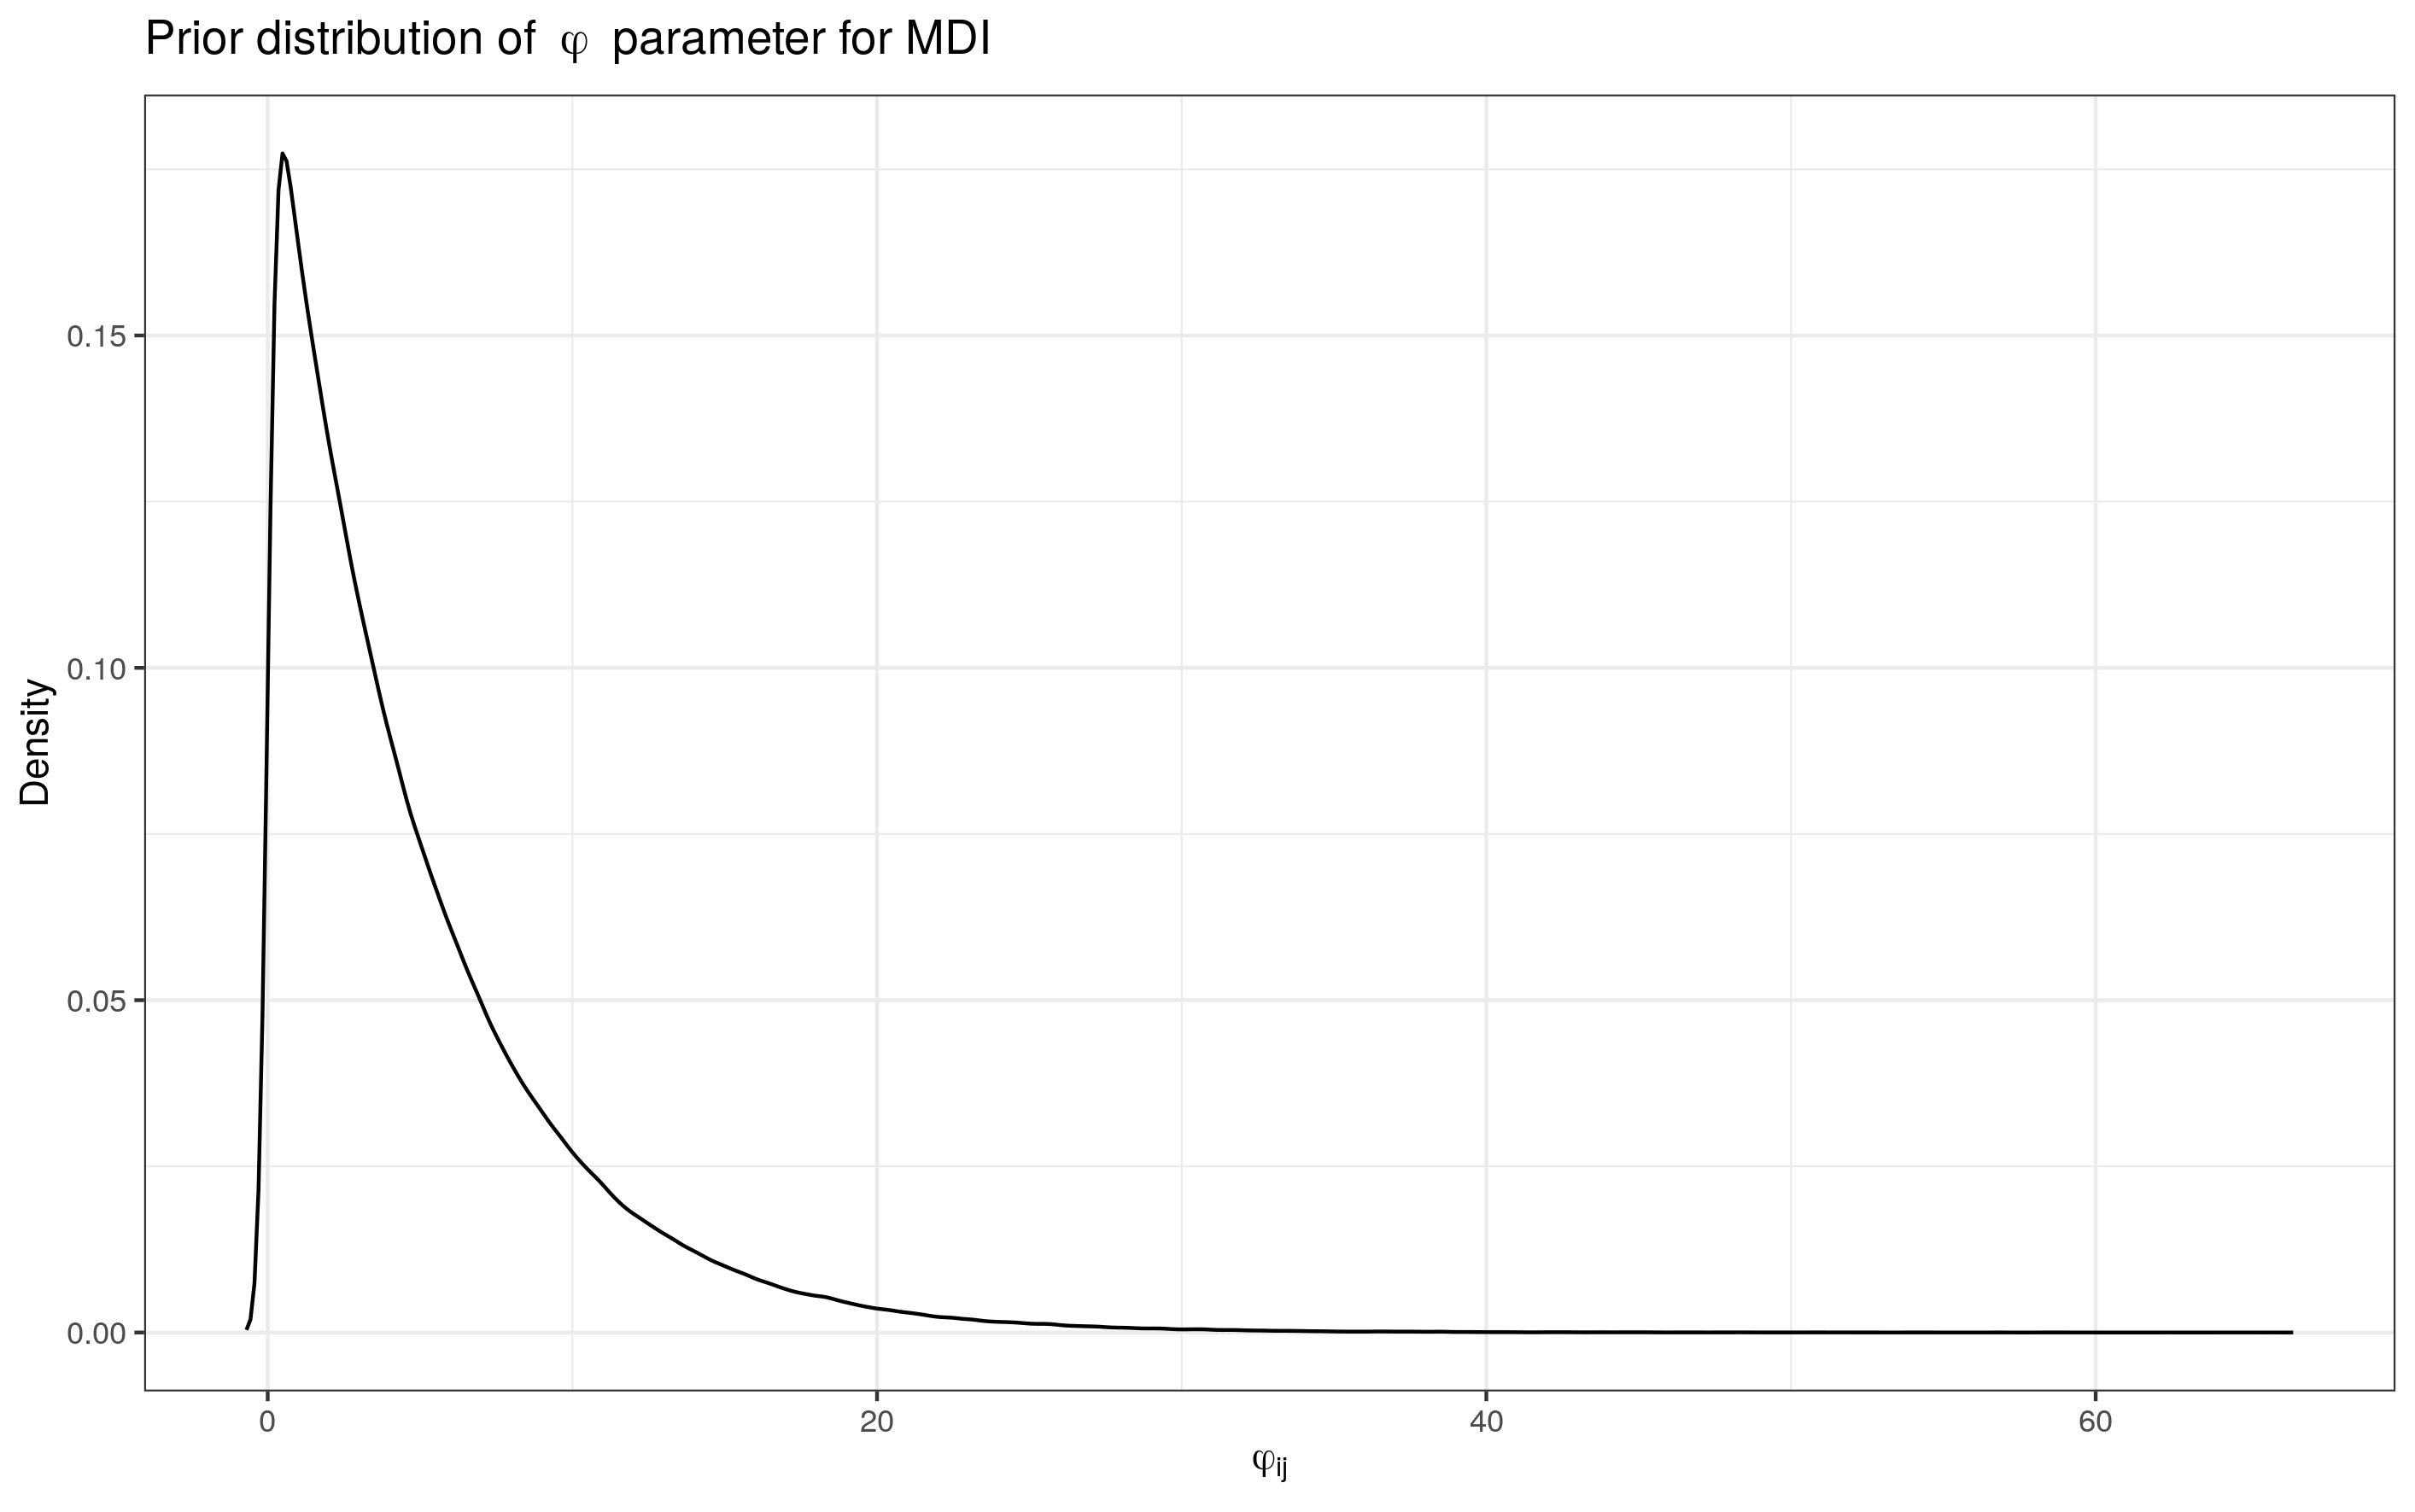
\includegraphics[scale=0.65]{Images/Data_inspection/phi_prior.png}
		\caption{Prior distribution of $\phi_{ij}$ parameter for MDI.}
		\label{fig:mdi_phi_prior}
	\end{figure}

	\begin{figure}[!htb]
		\centering
		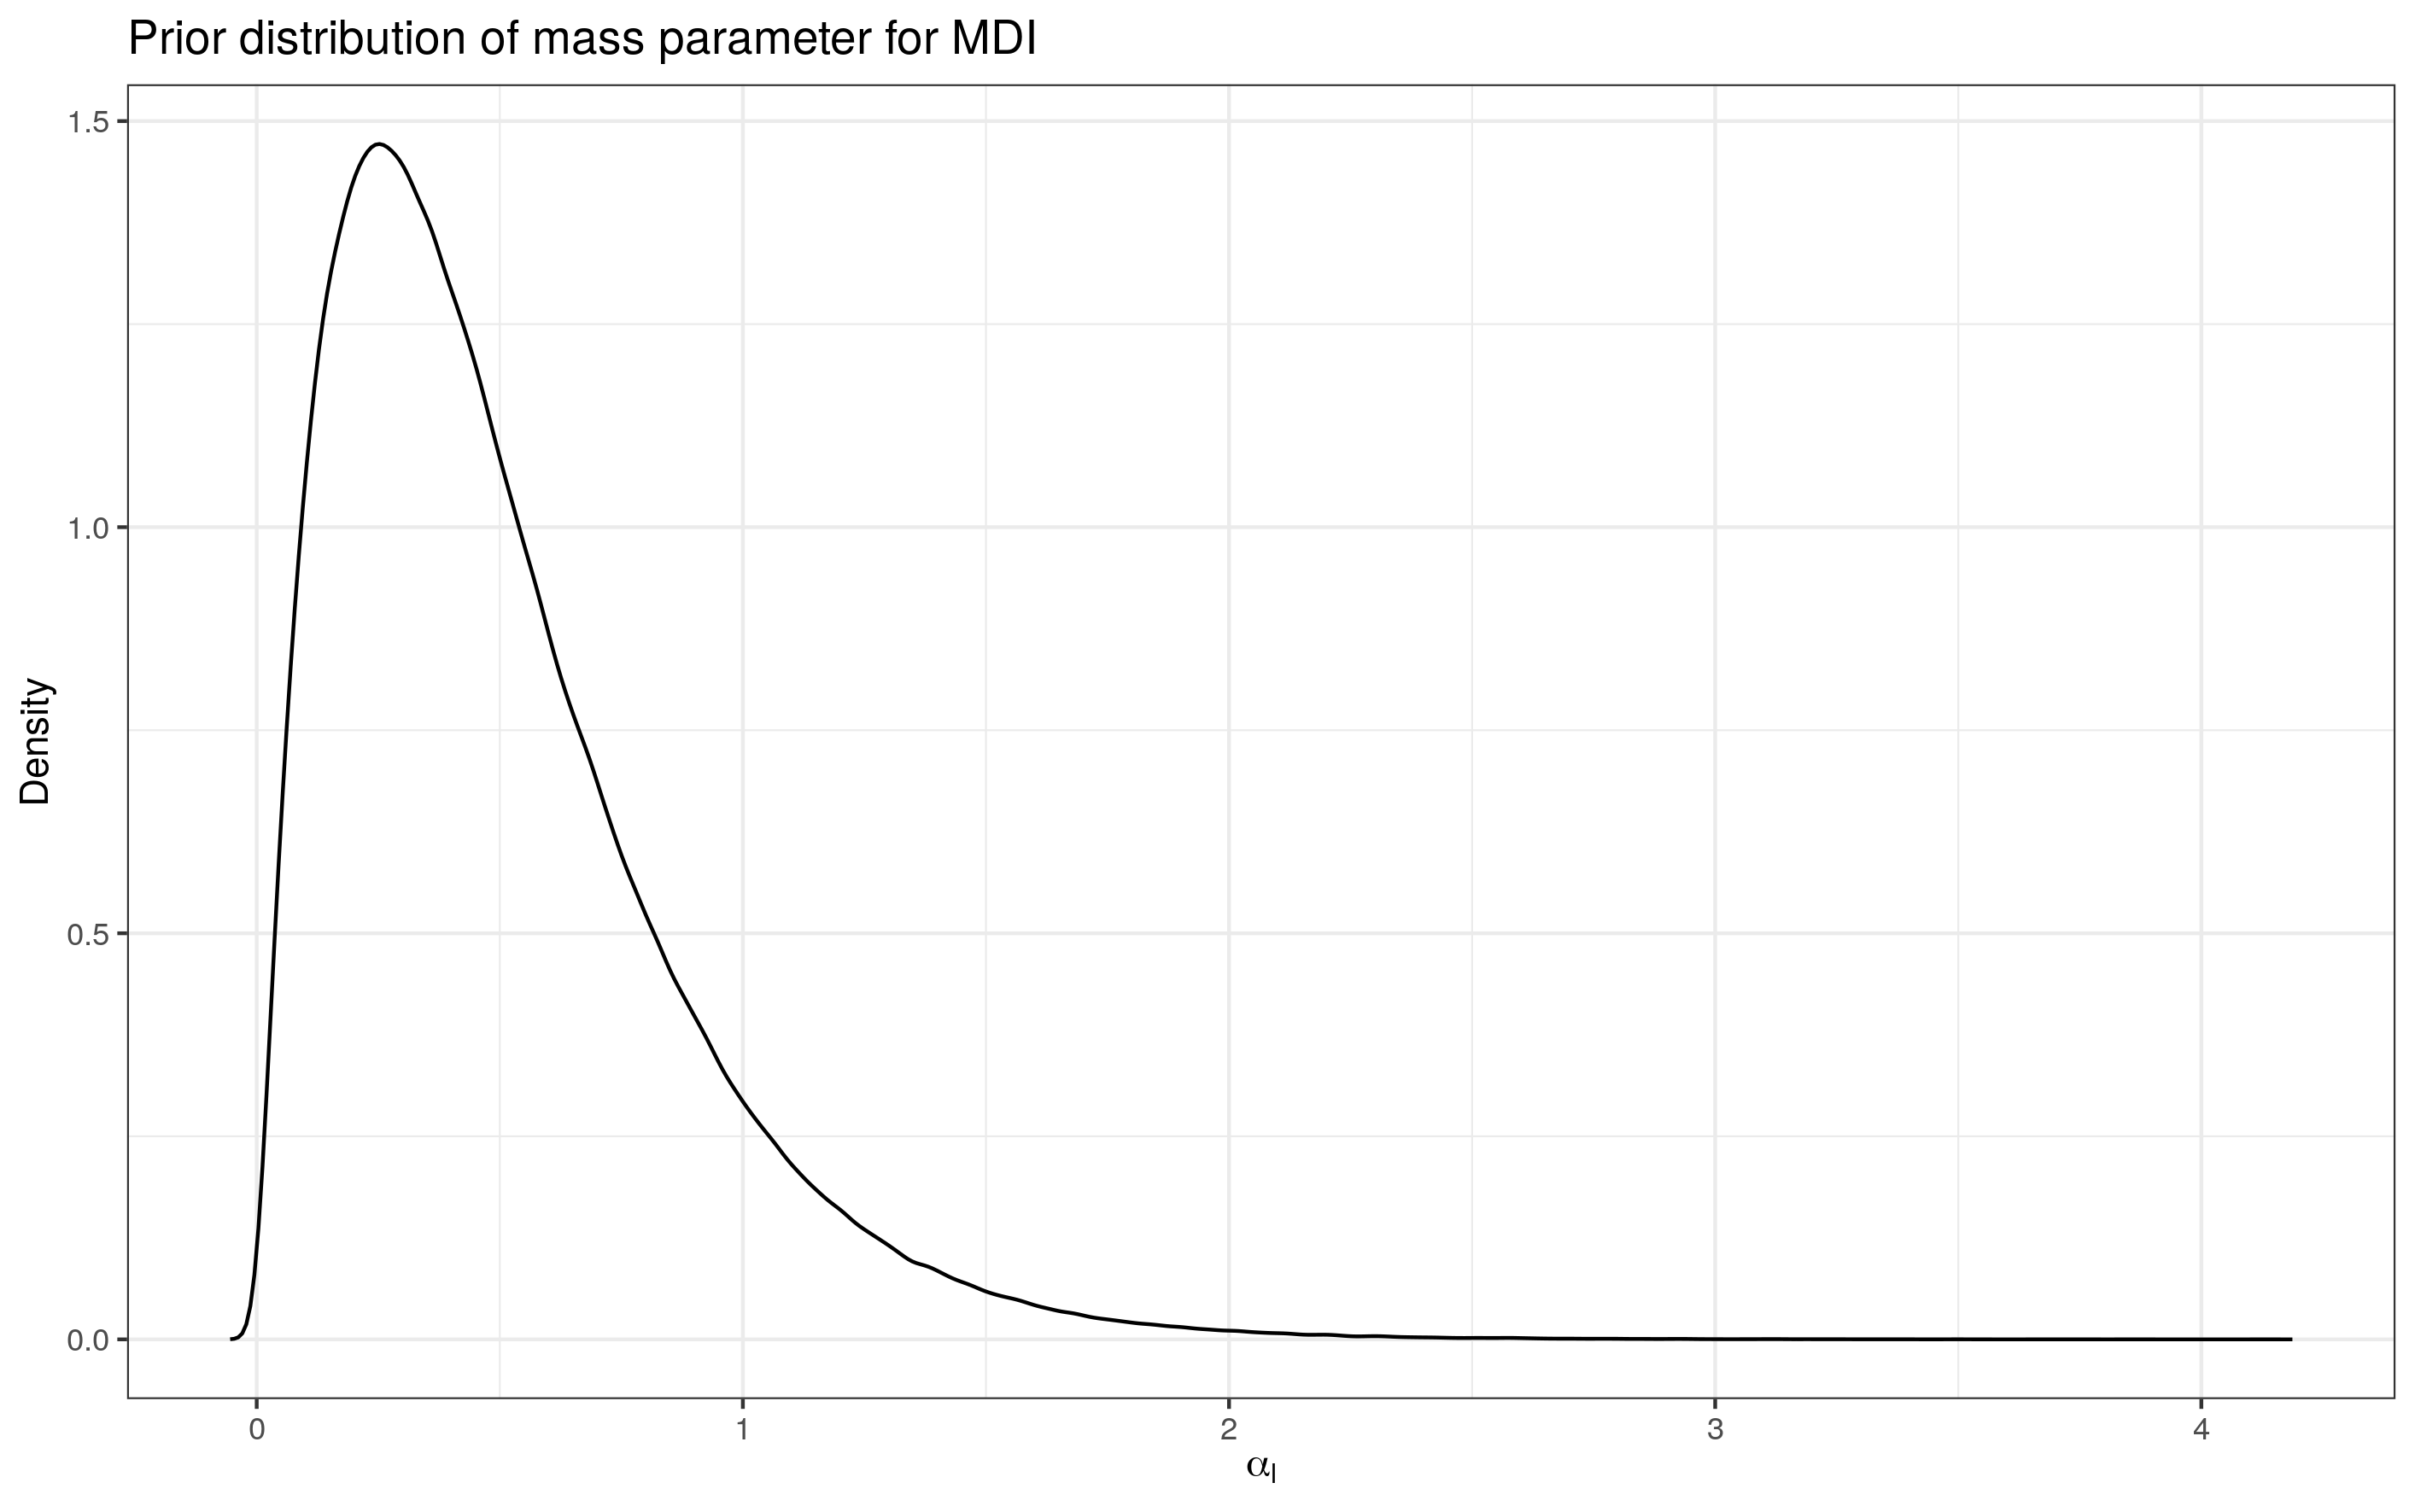
\includegraphics[scale=0.65]{Images/Data_inspection/alpha_prior.png}
		\caption{Prior distribution of $\alpha_l$ parameter for MDI.}
		\label{fig:mdi_alpha_prior}
	\end{figure}


	For the Gaussian density, it is assumed that each component is modelled by a Gaussian likelihood of unknown mean and  precision. A Normal-Gamma  prior is imposed upon these. The  density can therefore be represented in closed form and the mean and precision may be marginalised (one of the reasons the Gaussian distribution is easy to work with as referenced in section \ref{sec:theory:sub_sec:mixture_models}). This leaves the following marginal likelihood function for a component with $n$ genes allocated to it:
	\begin{align}
	f = \frac{\Gamma(\alpha_n)}{\Gamma(\alpha_0)} \frac{\beta_0 ^ {\alpha_0}}{\beta_n ^ {\alpha_n}} \left(\frac{\kappa_0}{\kappa_n}\right)^{\frac{1}{2}}\left(2\pi\right)^{-\frac{n}{2}}
	\end{align}
	Where:
	\begin{align}
		\mu &\sim \mathcal{N}(0, (\kappa_0 \lambda)^{-1}) \\
		\lambda &\sim \text{Ga}(\alpha_0, \beta_0) \\
		\kappa_n &= \kappa_0 + n \\
		\alpha_n &= \alpha_0 + \frac{n}{2} \\
		\beta_n &= \beta_0 + \frac{1}{2} \sum_{i=1}^n(x_i - \bar{x})^2 + \frac{\kappa_0 n \bar{x}^2}{2 \kappa_n}
	\end{align}
	The hyperparameters are set:
	\begin{align}
	\alpha_0 &=2 \\
	\beta_0 &= 0.5 \\
	\kappa_0 &= 0.001
	\end{align}
	These are intended to be broad, uniformed priors. This allows the model to infer from the data without an overtly strong influence from the priors.
		
	\subsection{Consensus clustering} \label{sec:consensus_clustering}
	In the scenario that MDI struggles to explore the entire posterior distribution from any given initialisation for any realistic number of iterations of MCMC, I propose use of a ``consensus clustering'' \citep{MontiConsensusClusteringResamplingBased} to perform approximate Bayesian inference. In this scenario I draw samples of clusterings from MCMC chains with different initialisations and use these clusterings to describe the target distribution. In practice this involves running $n_{seeds}$ different chains of MDI for a smaller number of iterations, $n_{iter}$, and burning out the first $n_{iter} - 1$ iterations. The clustering from the final iteration is then saved for this model.
	
	I then combine the clusterings from all $n_{seeds}$ within a PSM for the $n$ genes.  From this PSM a summary clustering may be calculated. The combination of different initialisations enables exploration of multiple maxima in the posterior density and thus provides a more informed clustering than a method liable to become trapped in a single mode. 
	
%	As the algorithm is not exploring the full space in any given iteration, we expect that the uncertainty quantification is optimistic. However we argue that an estimate made using insufficient data is better than one made using none at all and that this method is the best currently available to us for quantifying the uncertainty and exploring the posterior distribution.
	
	There have already been numerous applications of consensus clustering \citep{LiWeightedConsensusClustering2008, LancichinettiConsensusclusteringcomplex2012, BreimanRandomForests2001}. However, none of these previous implementations have used a Bayesian model. 
	

%	I show the validity of my implementation of consensus clustering by means of simulations. In this case I know the true clustering as I have chosen which points are drawn from which sub-populations I can then compare the quality of recorded clusterings generated by a single converged chain of MDI to different version of consensus clustering (i.e. varying $n_{iter}$). I let the quality of a clustering be defined by its similarity to the ground truth, measured using the \emph{adjusted Rand index} (see section \ref{sec:rand_index}).

	\subsection{Rand index} \label{sec:rand_index}
	A popular metric for comparing the similarity of two clusterings of the data is the \emph{Rand index} \citep{RandObjectiveCriteriaEvaluation1971}. If one assumes that all points are of equal importance in determining clusterings, then in combination with the discrete nature of clusters and the fact that a cluster is defined as much by what it does not contain as that which it does, \citet{RandObjectiveCriteriaEvaluation1971} proposed a metric to measure similarity between clusterings. If for the dataset $X=(x_1,\ldots,x_n)$ one is given two clusterings $Y=\{Y_1,\ldots,Y_{K}\}$ and $Y'=\{Y'_1,\ldots,Y'_{K'}\}$ with associated membership vectors $c=(c_1,\ldots,c_n)$ and $c'=(c_1'\ldots,c_n')$, then for any two points $x_i$ and $x_j$ there can exist one of a number of scenarios regarding their labelling. Let $\gamma_{ij}$ be a measure between the two points $x_i$ and $x_j$. For the two points, they can have:
	\begin{enumerate} \label{list:labelling_scenarios}
		\item The same label in both clusterings ($c_i = c_j \land c'_i = c'_j$) ($\gamma_{ij}=1$); \label{list:sub:same_label_1}
		\item Different labels in both ($c_i \neq c_j \land c'_i \neq c'_j$) ($\gamma_{ij}=1$); or \label{list:sub:same_label_2}
		\item The same label in one but not in the other ($c_i \neq c_j \land c'_i = c'_j \lor c_i = c_j \land c'_i \neq c'_j$) ($\gamma_{ij}=0$). \label{list:sub:different_label}
	\end{enumerate}
	Thus \citet{RandObjectiveCriteriaEvaluation1971} proposed counting the number of times any two points have one of \ref{list:sub:same_label_1} or \ref{list:sub:same_label_2} from list \ref{list:labelling_scenarios} and finding the proportion of these compared to the number of all possible point combinations. More formally, this is:
	\begin{eqnarray} \label{eqn:rand_index}
	A \binom{n}{2}^{-1} & = & \frac{1}{\binom{n}{2}} \sum_{i=1}^{n-1}\sum_{j=i + 1}^n\gamma_{ij} 
	\end{eqnarray}
	%	This is the quantity of points in agreement between the two clusters.
	This can be envisioned as a $K \times K'$ contingency table of the count of overlapping points, as shown in table \ref{table:rand_contingency}. Table \ref{table:rand_contingency} uses the following notation:
	\begin{itemize}
		\item $n_{ij}$ is the number of points that have membership in $Y_i$ in clustering $Y$ and $Y'_j$ in clustering $Y'$;
		\item $n_{\cdot j}$ is the number of points in cluster $Y'_j$ in clustering $Y'$;
		\item $n_{i \cdot}$ is the number of points in cluster $Y_i$ in clustering $Y$; and
		\item $n_{\cdot \cdot} = n$ is the number of points in clusterings $Y$ and $Y'$.
	\end{itemize}
	\begin{table}[] 
		\centering
		\begin{tabular}{c|cccc|c} 
			$ {{} \atop Y}  \!\diagdown\! ^{Y'}$	& $Y'_1$	& $Y'_2$	& $\cdots$	& $Y'_{K'}$	& Sums	\\ 
			\hline
			$Y_1$		& $n_{11}$	& $n_{12}$	& $\cdots$	& $n_{1K'}$	& $n_{1 \cdot}$	\\
			$Y_2$		& $n_{21}$	& $n_{22}$	& $\cdots$	& $n_{2K'}$	& $n_{2 \cdot}$	\\
			$\vdots$	& $\vdots$	& $\vdots$	& $\ddots$	& $\vdots$	& $\vdots$		 \\
			$Y_{K}$	& $n_{K1}$	& $n_{K2}$	& $\cdots$	& $n_{KK'}$	& $n_{K \cdot}$	\\ 
			\hline
			Sums	& $n_{\cdot 1}$	&  $n_{\cdot 2}$	& $\cdots$	& $n_{\cdot K'}$	& $n_{\cdot \cdot} = n$         
		\end{tabular}
		\caption{Contingency table used by \citet{RandObjectiveCriteriaEvaluation1971} to calculate a measure of similarity between clusterings $Y$ and $Y'$.}
		\label{table:rand_contingency}
	\end{table}
	One can restate equation \ref{eqn:rand_index} in terms of the notation from table \ref{table:rand_contingency} \citep{BrennanMeasuringagreementwhen1974}:
	\begin{eqnarray} \label{eqn:rand_index_alternative}
	A &=& \binom{n}{2} + \sum_{i=1}^K\sum_{j=1}^{K'}n_{ij}^2 - \frac{1}{2}\left(\sum_{i=1}^K n_{i\cdot}^2 + \sum_{j=1}^{K'}n_{\cdot j}^2  \right) \\
	&=& \binom{n}{2} + 2 \sum_{i=1}^{K}\sum_{j=1}^{K'}\binom{n_{ij}}{2} - \left[\sum_{i=1}^{K}\binom{n_{i \cdot}}{2} + \sum_{j=1}^{K'}\binom{n_{\cdot j}}{2}\right]% \binom{n}{2} ^{-1} 
	\end{eqnarray}
	%	This function, $c$, has three properties.
	%	\begin{itemize}
	%	\item $c(\cdot, \cdot) \in [0,1]$ (0 for no similarity, 1 for high similarity);
	%	\item $1 - c$ is a distance measure;
	%	\item if one assumes a distribution to describe $X$, then $c$ is a random variable.
	%	\end{itemize}
	\citet{HubertComparingpartitions1985} extend the Rand index to account for chance. They include a null hypothesis and assume that there is a probability of some points having a $\gamma$ value of 1 by chance. It can be shown that the expected number of points with common membership in both clusters is non-zero. Specifically:
	\begin{eqnarray}
	\mathbb{E}\left[\sum_{i=1}^K \sum_{j=1}^K\binom{n_{ij}}{2}\right] = \frac{\sum_{i=1}^K \binom{n_{i\cdot}}{2} \sum_{j=1}^K \binom{n_{\cdot j}}{2}}{\binom{n}{2}}
	\end{eqnarray}
	This is the product of the number of distinct pairs that can be formed from rows and the number of distinct pairs that can be constructed from columns, divided by the total number of pairs. 
	
	For a particular cell of the contingency table, the expected number of entries of the type described in point \ref{list:sub:same_label_1}, is the product of number of pairs in its row and in its column divided by the total number of possible pairs:
	\begin{eqnarray} \label{eqn:expected_nij}
	\mathbb{E}\left[\binom{n_{ij}}{2}\right] = \frac{\binom{n_{i\cdot}}{2}\binom{n_{\cdot j}}{2}}{\binom{n}{2}}
	\end{eqnarray}
	One can see that as each component of equation \ref{eqn:rand_index_alternative} is some transformation of $\sum_{i,j}\binom{n_{ij}}{2}$, one can directly state the expected value of the Rand index by combining equations \ref{eqn:rand_index_alternative} and \ref{eqn:expected_nij}:
	\begin{eqnarray}
	\mathbb{E}\left[A \binom{n}{2}^{-1}\right] = 1 + 2 \sum_{i=1}^{K} \binom{n_{i \cdot}}{2} \sum_{j=1}^{K'} \binom{n_{\cdot j}}{2} \binom{n}{2}^{-2} - \left[\sum_{i=1}^{K} \binom{n_{i \cdot}}{2} + \sum_{j=1}^{K'} \binom{n_{\cdot j}}{2}\right] \binom{n}{2}^{-1}
	\end{eqnarray}
	Defining an index corrected for chance as:
	\begin{eqnarray}
	\text{Corrected index} = \frac{\text{Index} - \text{Expected index}}{\text{Maximum index} - \text{Expected index}}
	\end{eqnarray}
	Assuming a maximum value of 1 for the Rand index then gives a corrected Rand index:
	\begin{eqnarray} \label{eqn:adjusted_rand_index}
	AR(Y, Y') &= \frac{\sum_{i=1}^{K}\sum_{j=1}^{K'} \binom{n_{ij}}{2} - \sum_{i=1}^{K} \binom{n_{i \cdot}}{2} \sum_{j=1}^{K'} \binom{n_{\cdot j}}{2} \binom{n}{2}^{-1}}{\frac{1}{2} \left[\sum_{i=1}^{K} \binom{n_{i \cdot}}{2} + \sum_{j=1}^{K'} \binom{n_{\cdot j}}{2}\right] - \sum_{i=1}^{K} \binom{n_{i \cdot}}{2} \sum_{j=1}^{K'} \binom{n_{\cdot j}}{2} \binom{n}{2}^{-1}}
	\end{eqnarray}
	This quantity is defined as the \emph{adjusted Rand index} and I use it as my measure of choice for similarity between clusterings.
	
	I describe an explicit example motivating the adjusted Rand index in section \ref{sec:motivating_example_adjusted_rand_index}.
	
	One can estimate the posterior expected adjusted Rand index from the recorded MCMC samples. \citet{FritschImprovedcriteriaclustering2009} suggest choosing the clustering $c^*$ that maximises the posterior expected adjusted Rand index. This is approximated from $n_{iter}$ MCMC samples by:
	\begin{align} \label{eqn:PEAR}
	\frac{1}{n_{iter}}\sum_{i=1}^{n_{iter}} AR(c^*, c^i)
	\end{align}
	Where $c^i$ is the $i^{th}$ recorded clustering. The R package mcclust \citep{FritschMcclust2012} includes a calculation of this quantity based upon the PSM.
	
	\subsection{Convergence}
	Assessment of convergence of Markov chains is a non-trivial issue. Apparent convergence can occur quite quickly when using a Gibbs sampler. \citet{ripley1990iterative} refer to a case when convergence was apparently achieved within several minutes, but then the algorithm jumped after a week of run-time. The following sub-sections briefly describe several heuristic measures to inspect convergence, but none are considered an absolute guarantee.
	
	\subsubsection{Auto-correlation} \label{sec:additional_theory:sub_sec:convergence:sub_sub_sec:autocorrelation}
	The autocorrelation, $\rho(i)$, is the correlation between the current sample and the sample at a lag of $i$. $\rho(0)=1$ as the observation correlates perfectly with itself. If the samples drawn are no longer correlated with previous samples this indicates the chain has achieved stationarity. For a deeper understanding of this, please see the description of Markov chains in section \ref{sec:additional_theory:sub_sec:gibbs_sampler}, specifically \eqref{eqn:stationary_distribution}.
	
	\subsubsection{Effective sample size} \label{sec:additional_theory:sub_sec:convergence:sub_sub_sec:ess}
	The Effective sample size (ESS) \citep{ripley2009stochastic} is an attempt to convert the number of MCMC samples, which can be highly autocorrelated, into an equivalent number of independent samples; consider it as an exchange rate. For $n$ samples and the letting $\rho(i)$ denote the correlation between the current sample and the sample drawn at a lag of $i$:
	\begin{align} \label{eqn:effective_smaple_size}
	ESS &= \frac{n}{1 + 2 \sum_{i=1}^\infty \rho(i)}
	\end{align}
	If the level of autocorrelation present is 0, then $ESS=n$;  if the autocorrelation decreases sufficiently slowly with regards to the lag that the sum in the denominator diverges, then $ESS=0$. One can use this to estimate the burn-in required to use samples only from the stationary distribution. One should use the burn-in at which ESS is maximised across all variables, as one wants to maximise the amount of samples available  while also ensuring one is sampling from the correct distribution.
		
	\subsubsection{Geweke $Z$-score} \label{sec:additional_theory:sub_sec:convergence:sub_sub_sec:geweke}
	\citet{GewekeEvaluatingAccuracySamplingBased} proposed a statistic based upon time-series methods to test the convergence. If the object of interest is a mean (which applies in the case of the continuous parameters of the MDI model) then this method is appropriate. The concept is based upon the belief that if the samples are all from the same distribution (i.e. the whole chain has converged), then the mean of the early samples should be similar to that from the later samples. To do this the samples are considered within two sets; the first $10\%$ and the last $50\%$ of the recorded samples.  The convergence statistic, $Z$, is the difference of the means associated with the samples from each set divided by the asymptotic standard error of their difference. As the number of samples recorded goes to infinity, the sampling distribution of $Z$ goes to $\mathcal{N}(0,1)$ if the chain has converged. Therefore the Geweke plot is inspected to see if many of the $Z$-scores occupy the extreme tails of the $\mathcal{N}(0,1)$ distribution.
	
	To construct the Geweke plot, the samples are split into disjoint bins. The first set of $\frac{n}{2(n_{bins} -1)}$ samples are placed in the first bin, the second set of $\frac{n}{2(n_{bins} -1)}$ samples in the second bin, etc. The final bin contains the final $50\%$ of samples. Geweke's $Z$-score is calculated comparing each bin of samples to the final $50\%$ of samples. The $Z$-scores are then plotted against the iteration number of the first iteration in each bin. If the chain has reached stationarity the Z-scores should be described by a standard normal distribution (in which case 95\% of the calculated $Z$-scores should be contained within the dashed lines in the plot, an example of which may be seen in figure \ref{fig:gen_data_case_1_geweke_plot_3}).
	
	
	\subsubsection{Gelman-Rubin shrink factor}
	\label{sec:additional_theory:sub_sec:convergence:sub_sub_sec:gelman}
	The approach described by \citet{GelmanInferenceIterativeSimulation1992} compares sequences across chains. If the chains are all sampling from the same distribution this is taken as evidence for convergence. This method tries to check if the samples from different chains are more different than would be expected based upon their internal variability; it does this by an analysis of the variance. Convergence is supported when the between-sequence variance $B$ is no larger than the within-sequence variance $W$.
	
	Consider a $m$ parallel chains, each of length $n$ of the variable $X$. Denote the chain specific samples by $x_i = (x_{i1},\ldots,x_{in})$. Then:
	
	\begin{align}
	B &= \frac{n}{m-1}\sum_{i=1}^m (\bar{x}_i - \bar{x})^2 \\
	W &= \frac{1}{m}\sum_{i=1}^m s_i^2
	\end{align}
	where $\bar{x}_i$ is the sample mean and $s_i$ is the sample standard deviation of the $i^{th}$ chain and $\bar{x}$ is the sample mean across chains, defined by:
	
	\begin{eqnarray} \label{eqn:sample_parameters}
	\bar{x}_i &=& \frac{1}{n}\sum_{j=1}^n x_{ij} \\
	s_i^2 &=& \frac{1}{n - 1}\sum_{j=1}^n \left( x_{ij} - \bar{x}_i \right) ^2 
	\end{eqnarray}
	From these variance components, it is expected that $W$ should be an estimate of $Var(X)$; a second estimate is constructed:
	\begin{align}
	\hat{Var}(X) = \frac{n-1}{n}W + \frac{1}{n}B
	\end{align}
	If the chains are stationary, this quantity $\hat{Var}(X)$ is an unbiased estimate of $Var(X)$, but if the starting points are over-dispersed it is an over-estimate.
	
	As $W$ should under-estimate $Var(X)$ for any finite value of $n$ (as the individual chains should not explore the full target distribution and thus will underestimate the variance present), there are two quantities estimating $Var(X)$ that should also impose the upper and lower bounds on $Var(X)$. Thus \citet{GelmanInferenceIterativeSimulation1992} proposed using the ratio of these quantities to estimate across-chain convergence. Specifically the estimated potential scale reduction or \emph{shrink factor}:
	\begin{align}
	\sqrt{\hat{R}} = \sqrt{\frac{\hat{Var}(X)}{W}}
	\end{align}
	As the chains converge, $\sqrt{\hat{R}}$ falls to 1. This means that the parallel Markov chains  are  essentially  overlapping.   If  the  shrink  factor  is  high,  then  one  should  proceed  with further simulations.
	


%	$\delta_{ij}$ here is the Kronecker delta and is defined:
%	
%	\begin{eqnarray}
%	\delta_{ij} =
%	    \begin{cases}
%	            1, &         \text{if } i=j,\\
%           	 0, &         \text{if } i\neq j.
%	    \end{cases}
%    	\end{eqnarray}
	
	%and $Y'=\left\{Y'_1,\ldots,Y'_{K'}\right\}$
	
%	\subsection{Expression quantitative trait loci}
%	The last two decades have seen a huge body of research focused on genome variability due to its 
%	relevance in the risk of disease experienced by individuals. Fundamental to this study is 
%	understanding the effect different genome variants have; i.e. understanding how this change 
%	in genome translates to a different phenotype. This means we must investigate the change a 
%	variant effects within the cell. Ideally this information allows biological insight into the 
%	aetiology and nature of disease or of the phenotype. Genome-wide association studies (GWAS) 
%	\citep{feero_genomewide_2010} have shown that the majority of these variants are located within 
%	the non-coding regions of the genome \citep{NicaExpressionquantitativetrait2013} implying that they are involved in gene regulation. These 
%	sites that explain some of the phenotypic variance are referred to as expression quantitative 
%	trait loci (eQTL).
%	
%	eQTLs have transformed the study of genetics. They provide a comprehensible, accessible and 
%	most importantly interpretable molecular link between genetic variation and phenotype. Standard 
%	eQTL analysis involves a direction association test between markers of genetic variation, 
%	typically using data collected from tens to hundreds of people.
%	
%	This analysis can be proximal or distal.
%	\begin{itemize}
%		\item Proximal: immediately responsible for causing some observed result;
%		\item Distal: (also \emph{ultimate}) higher-level than proximal. The true cause for an event or 
%		result.
%	\end{itemize}
%	Consider the example of a ship sinking. This could have a \emph{proximate} cause such as the ship 
%	being holed beneath the waterline leading to water entering the ship; this resulted in the ship 
%	becoming denser than water and it sank. However, the \emph{distal} cause could be the ship hit a 
%	rock tearing open the hull leading to the sinking.
%	
%	In terms of eQTLs, we designate proximal effects as \emph{cis-eQTL} and distal causes as 
%	\emph{trans-eQTL}. We normally consider an eQTL to be cis-regulating if it is within 1MB of the 
%	gene transcription start site (TSS) and trans-regulating if it is more than 5MB upstream or 
%	downstream of the TSS or if found on a different chromosome \citep{NicaExpressionquantitativetrait2013}.
%	
%	trans-eQTL are hard to find. They have weaker effects than cis-eQTL and thus require greater power 
%	in the experiment \citep{dixon_genome-wide_2007}. For some context, \citet{burgess_gene_2017} claims 
%	that 449 donors provide low power in terms of finding trans-eQTL. As the power of experiments increases 
%	more trans-eQTL are observed and cis-eQTL are shown to be generally tissue agnostic 
%	\citep{GTExConsortiumGeneticeffectsgene2017}. Previous results suggested cis-eQTL would be have tissue specific effects, 
%	but the increase in experimental power revealed that this is not the case \citep{GrundbergMappingcistransregulatory2012}. 
%	The current power present in many genetic experiments is enough to observe trans-eQTLs and indicates 
%	these have tissue specific properties \citep{GrundbergMappingcistransregulatory2012, GTExConsortiumGeneticeffectsgene2017}. It is possible that this result might be shown as an artefact of insufficient power, much as initial analysis suggested cis-eQTL had tissue specific properties. However, for now we assume it is true and that trans-eQTL are more likely to display tissue specific behaviour 
%	than cis-eQTL.
	
%	\subsection{Tissue specificity} \label{sec:tissue_specificity}
%	Cell-type specific gene pathways are pivotal in differentiating tissue function, implicated in hereditary organ failure, and mediate acquired chronic disease \citep{JuDefiningcelltypespecificity2013a}. More and more evidence is being accrued to highlight the cell-type specific level of gene expression \citep{GrundbergMappingcistransregulatory2012, OngEnhancerfunctionnew2011, ManiatisRegulationinducibletissuespecific1987}. 
%	
%%	Beyond healthy variation in gene expression across tissues, in the  area of immunology many diseases are tissue specific and have strong associations to genetic pre-disposition
%	
%	We also see that there are many auto-immune disease, normally associated with a specific tissue type, that have strong genetic associations. Tissue specific isoforms and expression have also been observed \citep{WangAlternativeisoformregulation2008a}. This shows that genes have context-specific interactions that should be considered in analysis.
	
%	\subsection{Gene sets}
%	Analysing pre-defined gene sets and changes in the expression of the full set rather than considering each constituent member on an individual basis has more statistical power \citep{MooneyGenesetanalysis2015}. Consider, that in analysing gene sets as a group, the degree of perturbation in the expression of the full gene set due to the disease state / alternative phenotype that is required to be considered significant is much less than that required in analysing each of its constituent members individually \citep{DudbridgePowerPredictiveAccuracy2013, WrayResearchReviewPolygenic2014}.
	
%	I identify gene sets based upon common patterns of expression. Correlated expression (or co-expression) between genes is often an indicator that they are:
%	\begin{itemize}
%		\item Controlled by the same transcription factor;
%		\item Functionally related; or
%		\item Members of the same pathway \citep{WeirauchGeneCoexpressionNetworks2011}.
%	\end{itemize}
%	As this correlated expression is represented by a common variation across people (or experimental conditions) rather than in the magnitude of expression, I will standardise the expression data as described in section \ref{sec:standardisation}. I describe a small example to highlight my reasoning in section \ref{sec:motivating_example_standardisation}.
	
%	Furthermore, it is known from Genome Wide Association Studies that many diseases are polygenic in nature \citep{MooneyGenesetanalysis2015}. This suggests that it is natural to be considering sets of genes in analysis of many diseases. \citet{SubramanianGenesetenrichment2005a} highlight the importance of gene sets, claiming that within a single metabolic pathway an increase of $20\%$ in all the associated gene products may have more impact upon phenotype than a 20-fold increase in a single gene. Thus gene sets have more relevance than individual genes to biological impact - furthermore the interpretation of gene sets in the context of pathways is a step closer to phenotype than the information encoded in individual genes. As a deeper biological understanding of the phenotype or disease state is the aim, this encourages the use of gene sets.
	
%	Analysing pre-defined gene sets increases the statistical power of an analysis\citep{MooneyGenesetanalysis2015}. As I have stated previously, analysis of the set requires less perturbation of expression for significance than analysis of an individual. There is also no obvious detriment in analysing gene sets - no loss of information found. As the gene sets are expected to have correlated expression \citep{WeirauchGeneCoexpressionNetworks2011}, one expects that if the expression of a gene within the set does change then, if this is not due to noise or stochasticity, the expression of other members of the set should should also vary accordingly.
	
%	Thus clustering genes into groups known as ``gene sets'' is natural and useful from both a biological and statistical perspective - it can increase the interpretability and the power of an analysis \citep{NicaExpressionquantitativetrait2013, VosaUnravelingpolygenicarchitecture2018}.
	
%	\subsubsection{Tissue specificity}
%	The problem of defining gene sets is non-trivial with many variations in-use. There exist many databases of gene sets \citep{AshburnerGeneOntologytool2000a, KanehisaNewapproachunderstanding2019, SzklarczykSTRINGv11protein2019}. The Molecular Signature Database \citep{SubramanianGenesetenrichment2005a} (MSigDB) is one of the most popular resources for GSEA and encompasses many different gene sets defined under various criteria or generated from separate resources.
%	
%	However, none of these definitions of a ``set'' incorporate tissue specific information. This seems an oversight. Cell-type specific gene pathways are pivotal in differentiating tissue function, implicated in hereditary organ failure, and mediate acquired chronic disease \citep{JuDefiningcelltypespecificity2013a}. More and more evidence is being accrued to highlight the cell-type specific level of gene expression \citep{GrundbergMappingcistransregulatory2012, OngEnhancerfunctionnew2011, ManiatisRegulationinducibletissuespecific1987}. Thus we propose defining tissue specific gene sets. 
	
%	EXPAND THIS SECTION
	
%	There is specific interest in defining gene sets annotated with tissue or cell type specific information. Previous attempts to achieve this have used the Genotype Tissue Expression (GTEx) \citep{GTExConsortiumGeneticeffectsgene2017} database \citep{LonsdaleGenotypeTissueExpressionGTEx2013}, but here the profiles are for human donors
%	post-mortem. One might suspect that the data derived from these cells may not contain the same information as that collected from living, active cells. Furthermore, the GTEx data is across many different tissues (144 are used in \citep{LonsdaleGenotypeTissueExpressionGTEx2013}), but I focus on cell types relevant to autoimmune disease in general (i.e. white blood cells) and Inflammatory Bowel Disease in particular (intestinal samples).
%	
%	I AM NOT SURE ABOUT THIS:
%	
%	I am of the opinion that in an exploration of a concept (as described here) one should focus on a smaller dataset to enable analysis and interpretation; if one uses a mountain of data and compares across enough cases one is quite likely to find some sort of evidence for an argument. Defining the argument in advance, restricting the options available for exploration and uncovering evidence in this context is something I find more convincing. Thus, a smaller, restricted dataset is considered.
	
%	With the onset of microarrays and RNAseq, producing gene expression data in large quantities for a wide number of genes is increasingly enabled. Unfortunately the large amount of data gifted onto the genomics community by these methods is difficult to interpret and analyse. Gene Set Enrichment Analysis (GSEA) attempts to overcome some of these issues by using prior knowledge to define groups of genes linked through their biological function \citep{HejblumTimeCourseGeneSet2015}. The set is defined using knowledge external to the current analysis; a common method is using the manually annotated pathways available on the Kyoto Encyclopedia of Genes and Genomes (KEGG) database \citep{FridleyGenesetanalysis2011}.
%		
%	Analysing pre-defined gene sets and changes in the expression of the full set rather than considering each constituent member on an individual basis has more statistical power \citep{MooneyGenesetanalysis2015}. Consider, that in analysing gene sets as a group, the degree of perturbation in the expression of the full gene set due to the disease state / alternative phenotype that is required to be considered significant is much less than that required in analysing each of its constituent members individually \citep{DudbridgePowerPredictiveAccuracy2013, WrayResearchReviewPolygenic2014}.
%	
%	We know from Genome Wide Association Studies (GWAS) that many diseases are polygenic in nature \citep{MooneyGenesetanalysis2015}. This suggests that it is natural to be considering sets of genes in analysis of many diseases. \citet{SubramanianGenesetenrichment2005a} highlight the importance of gene sets, claiming that within a single metabolic pathway an increase of $20\%$ in all the associated gene products may be more important than a 20-fold increase in a single gene.
%	
%	Thus clustering genes into groups known as ``gene sets'' is natural and useful from both a biological and statistical perspective - it can increase the interpretability and the power of an analysis \citep{NicaExpressionquantitativetrait2013, VosaUnravelingpolygenicarchitecture2018}.
%	
%	However, the problem of defining gene sets is non-trivial with many variations in-use. There exist many databases of gene sets \citep{AshburnerGeneOntologytool2000a, KanehisaNewapproachunderstanding2019, SzklarczykSTRINGv11protein2019}. The Molecular Signature Database \citep{SubramanianGenesetenrichment2005a} (MSigDB) is one of the most popular resources for GSEA and encompasses many different gene sets defined under various criteria or generated from separate resources. However, none of these definitions of a ``set'' incorporate tissue specific information. We believe that this is an oversight as there is evidence that some genes are involved in tissue specific pathways (see section \ref{sec:tissue_specificity}). Thus we propose defining tissue specific gene sets. Previous attempts to achieve this have used the Genotype Tissue Expression (GTEx) \citep{GTExConsortiumGeneticeffectsgene2017} database \citep{LonsdaleGenotypeTissueExpressionGTEx2013}, but here the profiles are for human donors
%	post-mortem. We suspect that the data derived from these cells may not contain the same information as that collected from living, active cells. Furthermore, the GTEx data is across many different tissues (144 are used in \citep{LonsdaleGenotypeTissueExpressionGTEx2013}), but we focus on cell types relevant to autoimmune disease in general (i.e. blood cells) and IBD in particular (intestinal samples). This restricted focus should offer relevant gene sets.
%	
%	Gene sets should contain sets of genes that have correlated expression. If this is the case, it is often assumed that the genes are common members of some metabolic pathway and that their products interact. As this correlated expression is represented by a common variation across people rather than in the magnitude of expression, we will standardise the expression data as described in section \ref{sec:standardisation}. We describe a small example to highlight our reasoning in section \ref{sec:motivating_example_standardisation}.
	

%	\subsection{The importance of gene sets}
%	If we can cluster genes together it is possible that we can find deeper biological interpretation, understanding the context of the gene products and what they interact with. This can offer some insight into the connection between the gene and the expressed phenotype. Furthermore, \citet{NicaExpressionquantitativetrait2013} recommend investigating groups of cis-eQTL affecting a gene network that when perturbed results in a disease state. They claim this is far higher powered than the classical approach. This claim is supported by the findings of \citet{VosaUnravelingpolygenicarchitecture2018} who found that associations between \emph{polygenic risk scores} and gene expression (this association is referred to as ``expression quantitative trait score'' (eQTS) in \citep{VosaUnravelingpolygenicarchitecture2018}) contained the most biological information about disease in a comparison of cis-eQTL, trans-EQTL and eQTS. This finding is not unique to this paper \citep{DudbridgePowerPredictiveAccuracy2013, WrayResearchReviewPolygenic2014}. More generally, gene set enrichment analysis (GSEA) \citep{SubramanianGenesetenrichment2005a, MooneyGenesetanalysis2015} relies upon pre-defined gene sets. This method determines if gene sets have statistically significant, concordant differences between phenotypes and offers biological interpretation of the sets. Thus well-defined gene sets are required for informative, interpretable analysis of genomic information.
	
	
%	\subsection{Existing databases}
%	There exist many databases of gene sets \citep{AshburnerGeneOntologytool2000a, KanehisaNewapproachunderstanding2019, SzklarczykSTRINGv11protein2019}. The Molecular Signature Database \citep{SubramanianGenesetenrichment2005a} (MSigDB) is one of the most popular resources for GSEA and encompasses many different gene sets defined under different criteria or generated from different resources. However, none of these definitions of a ``set'' incorporate tissue specific information. 
%	(such as the Gene Ontology (GO) Resource \citep{AshburnerGeneOntologytool2000a}, the Kyoto Encyclopedia of Genes and Genomes (KEGG) \citep{KanehisaNewapproachunderstanding2019}, the Molecular Signatures Database (MSigDB) \citep{SubramanianGenesetenrichment2005a} or the STRING protein-protein interaction (PPI) database \citep{SzklarczykSTRINGv11protein2019})
	
	

%	\subsection{Variance stabilisation}
	
	\subsection{Standardisation} \label{sec:standardisation}
	As I have chosen to define gene sets by co-expression, which is represented by a common variation across people (or experimental conditions) rather than in the magnitude of expression, I standardise the data.
	
	For a $p$-vector of observations, $X_i=(x_{i1},\ldots,x_{1p})$, standardisation of $X_i$ is defined as the mapping from $X_i$ to $X'_i=(x'_{i1},\ldots,x'_{ip})$ defined by the sample mean, $\bar{x}_i$, and sample standard deviation, $s_i$ calculated as described by \eqref{eqn:sample_parameters}. Then:
	\begin{eqnarray} \label{eqn:standardisation}
%	\bar{x}_i &=& \frac{1}{p}\sum_{j=1}^p x_{ij} \\
%	s_i^2 &=& \frac{1}{p - 1}\sum_{j=1}^p \left( x_{ij} - \bar{x}_i \right) ^2 \\
	x'_{ij} &=& \frac{x_{ij}- \bar{x}_i}{s_i} \; \forall \; j \in (1,\ldots,p)
	\end{eqnarray}
	I refer to $X'_i$ as the standardised form of $X$. If one is given a dataset $X=(X_1,\ldots,X_n)$ where each $X_i$ is a $p$-vector of observations of the form referred to above, then in referring to the standardised form of $X$, I mean the dataset $X'=(X'_1,\ldots,X'_n)$ where each $X'_i$ is the standardised form of $X_i$.
	
	Standardisation moves the values observed for each $X_i$ to a common scale where each vector has an observed mean and standard deviation of 0 and 1 respectively. A motivating example in the context of gene expression data is described in section \ref{sec:motivating_example_standardisation}.

	\section{Case study examples}
	I first show via simulated data that consensus clustering does produce similar results to a converged single run for MDI.
	
	I then simulate data where individual chains of MDI are expected to struggle to converge and possibly will not converge in finite time. I show that consensus clustering explores a wider space than any individual chain and appears to describe something similar to the space described by the union of the chains.
	
	Finally I apply consensus clustering to two sets of probes for 7 tissue or cell-type specific datasets from the CEDAR dataset; a set of 250 probes with a single KEGG pathway present and a set of 1,000 probes with three KEGG pathways present.
	
	\subsection{Simulations}
	\subsubsection{Simulation: Case 1} \label{sec:sim:data:case_1}
	The data in the first simulation is designed to allow MDI to converge. In this case I take the data generated for the original MDI paper \citep{KirkBayesiancorrelatedclustering2012}. As this data is highly separable I add some noise to add some uncertainty to the clustering. 
	
	In this case I have 3 datasets (MDItestdata1, MDItestdata2 and MDItestdata3). I use MDItestdata1 as the basis to define new data. I generate two overlapping clusters (cluster 8 and 9) defined by two of the original clusters (cluster 4 and 6). One can see the correlation structure for this data in figure \ref{fig:cor_matrix_1_sim_case_1}.
	
	I define clusters 8 and 9 to be generated from a MVN distribution with a mean defined by the weighted means of clusters 4 and 6 and a variance defined by the weighted variance of these same clusters. For cluster 8 the relative weights are 0.6 and 1 for clusters 4 and 6. The weights are reversed for cluster 9, this means cluster 9 is more similar to cluster 4 whereas 8 is closer to cluster 6. 
	
	\begin{figure}[!htb]
		\centering
		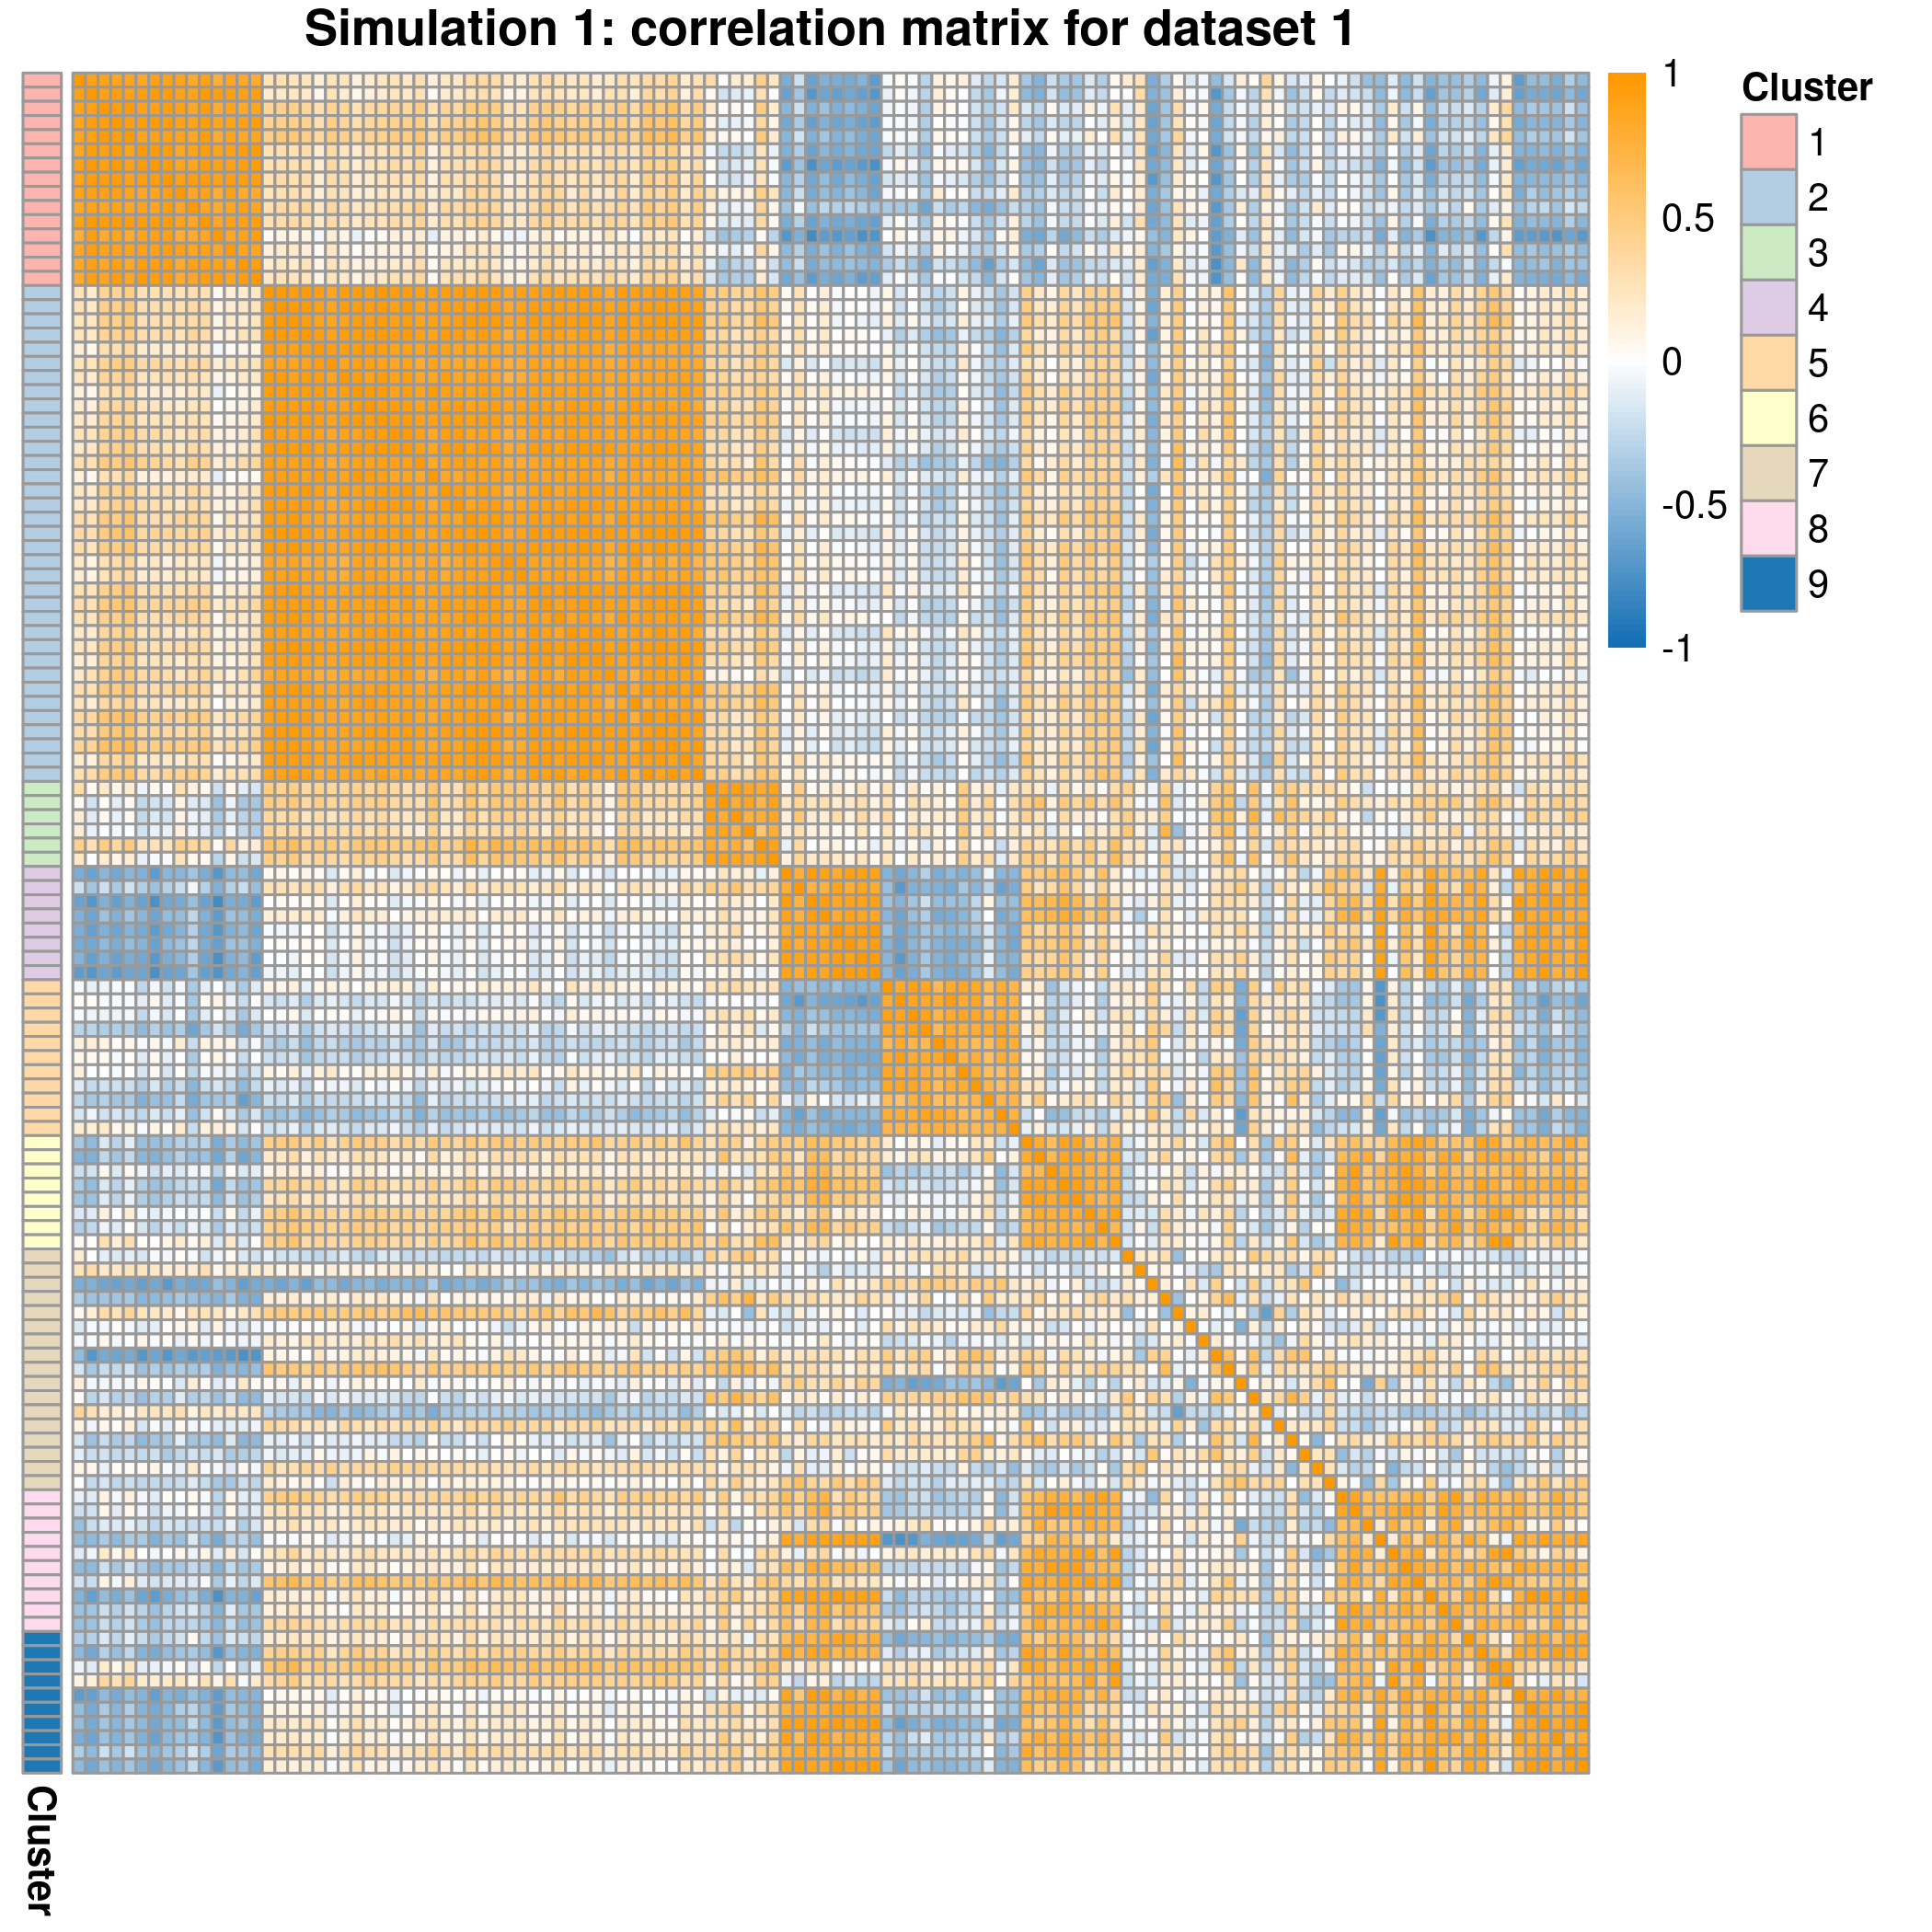
\includegraphics[scale=0.65]{Images/Gen_data/Case_1/cor_matrix_dataset_1.png}
		\caption{Heatmap of correlation matrix for the first simulation annotated by the ``true" labelling, as described in section \ref{sec:sim:data:case_1}. One can see that the first 7 clusters are quite separable, but the introduction of the $8^{th}$ and $9^{th}$ creates uncertainty in the membership for a clustering model.}
		\label{fig:cor_matrix_1_sim_case_1}
	\end{figure}
	
	\subsubsection{Simulation: Case 2} \label{sec:sim:data:case_2}
	The data in the second simulation is designed to be a testing example in which MDI might struggle to converge. This data is based upon 5 clusters of $n_{clust}=\{25, 50, 75, 100, 150\}$ genes (let $n_{clust_i}$ be the number of genes in the $i^{th}$ cluster) for $p=400$ people. Each cluster is defined by a MVN distribution with common variance of 1. I then perturb the clusters, adding a small amount of noise generated from a normal distribution of mean 0 and standard deviation 0.1. This noise makes the clusters less distinct. I generate 3 datasets this way, varying the means defining the clusters between datasets (as can be seen in table \ref{table:generated_data_case_2}).
	
	\begin{table}[!htb] 
		\centering
		\begin{tabular}{c|c|ccc} 
			Cluster & $n_{clust}$	& Dataset 1	& Dataset 2	& Dataset 3	\\ 
			\hline
			1 		&	25 		& $\mathcal{N}(1,1)$	& $\mathcal{N}(1,1)$ 	& $\mathcal{N}(1,1)$	\\
			2 		&	50		& $\mathcal{N}(2,1)$	& $\mathcal{N}(3,1)$ 	& $\mathcal{N}(1.5,1)$	\\
			3 		& 	75		& $\mathcal{N}(4,1)$	& $\mathcal{N}(6,1)$ 	& $\mathcal{N}(3,1)$	\\
			4 		&	100		& $\mathcal{N}(6,1)$	& $\mathcal{N}(9,1)$ 	& $\mathcal{N}(4,1)$	\\
			5 		&	150 	& $\mathcal{N}(8,1)$	& $\mathcal{N}(12,1)$ 	& $\mathcal{N}(5,1)$	
		\end{tabular}
		\caption{Sub-populations defining the simulated data in case 2.}
		\label{table:generated_data_case_2}
	\end{table}
	
	More specifically the $i^{th}$ subpopulation in the $j^{th}$ dataset is defined by combining $p$ samples of $n_{clust_i}$ genes where each sample is pulled from the distribution described by the corresponding entry of table \ref{table:generated_data_case_2}. These samples are then perturbed by a random sample drawn from $\mathcal{N}(0,0.1)$. I expect that the underlying structure should be easiest to uncover in dataset 2 and hardest to uncover in dataset 3 (based upon the distance between the means used to define the different sub-populations for these datasets). One can obtain some insight into the uncertainty of membership for dataset 3 in figure \ref{fig:gen_data_3_sim_case_2}.



	\begin{sidewaysfigure} %[!htb]
		\centering
		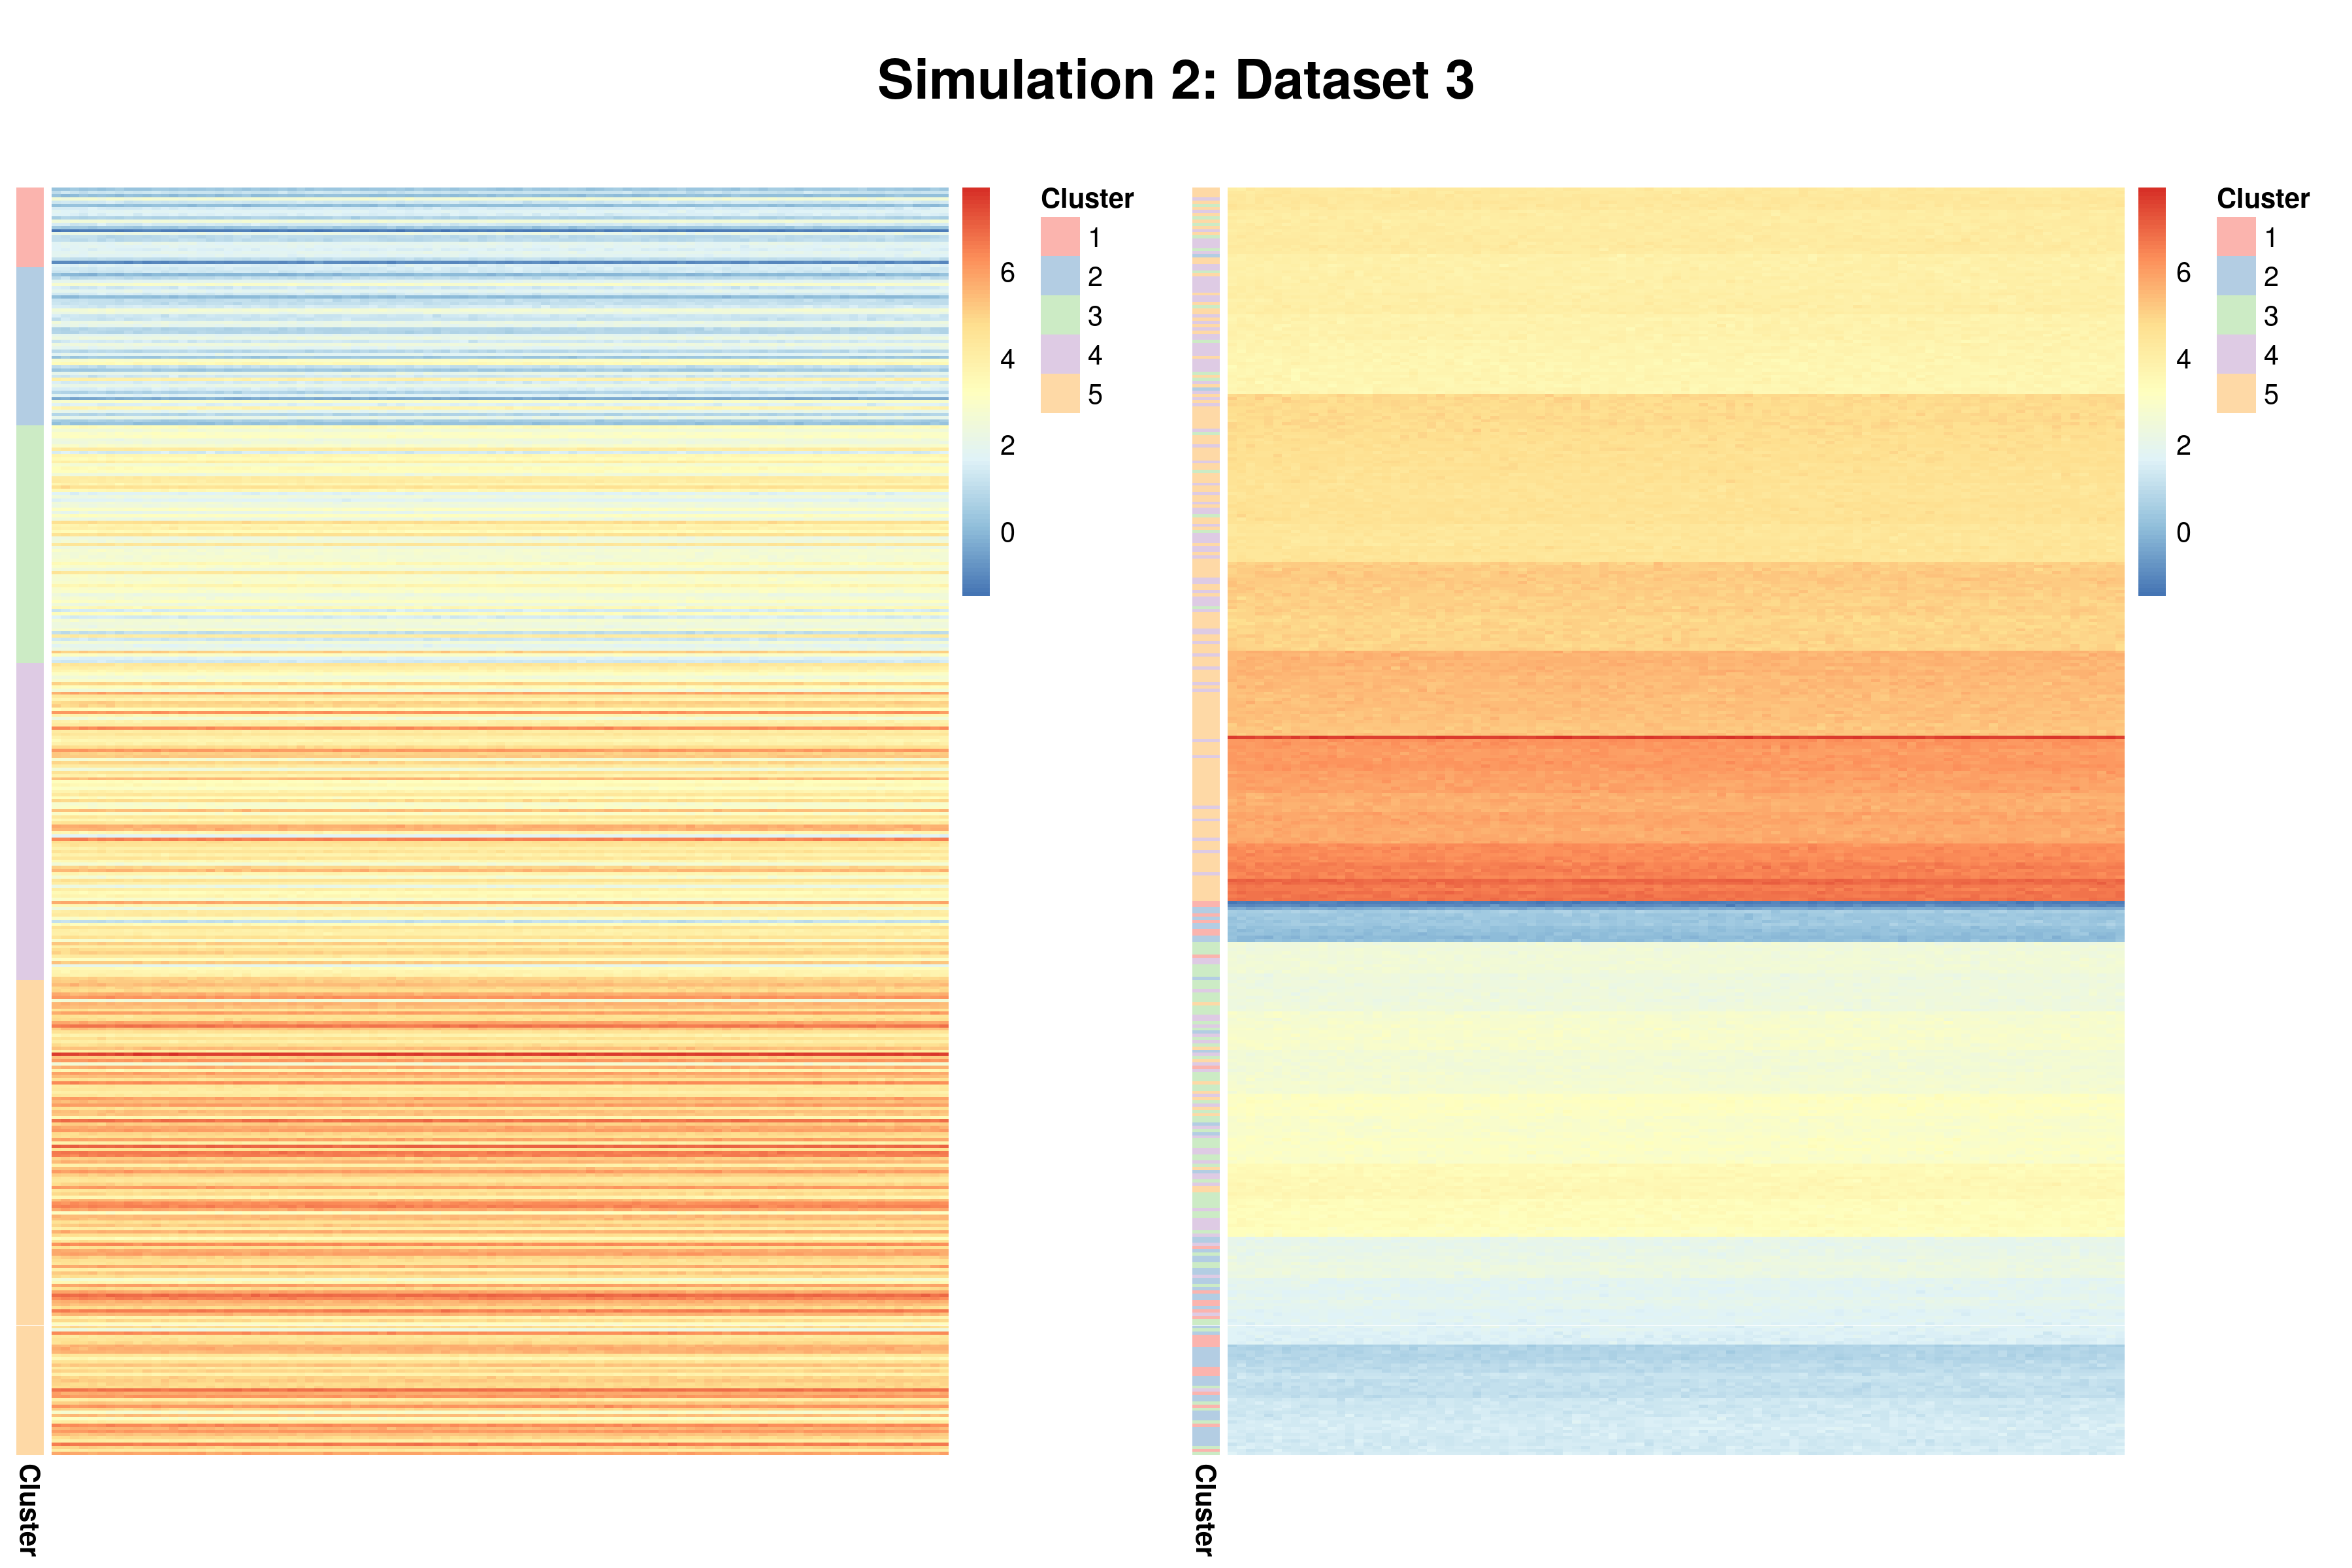
\includegraphics[scale=0.7]{Images/Gen_data/Case_2/dataset_3_comp_clustered_unclustered.png}
		\caption{Heatmap of expression data generated for the third dataset of the second simulation as described in section \ref{sec:sim:data:case_2}, annotated by the true clustering. On the left the data is ordered by the true labelling, on the right ordering is defined by the structure within the data as recognised by a hierarchical clustering model. Note that there are 5 populations present here and that cluster membership and boundaries are not obvious; due to this I expect the clustering model to struggle to uncover the true structure.}
		\label{fig:gen_data_3_sim_case_2}
	\end{sidewaysfigure}

%\begin{figure}[!htb]
%	\centering
%	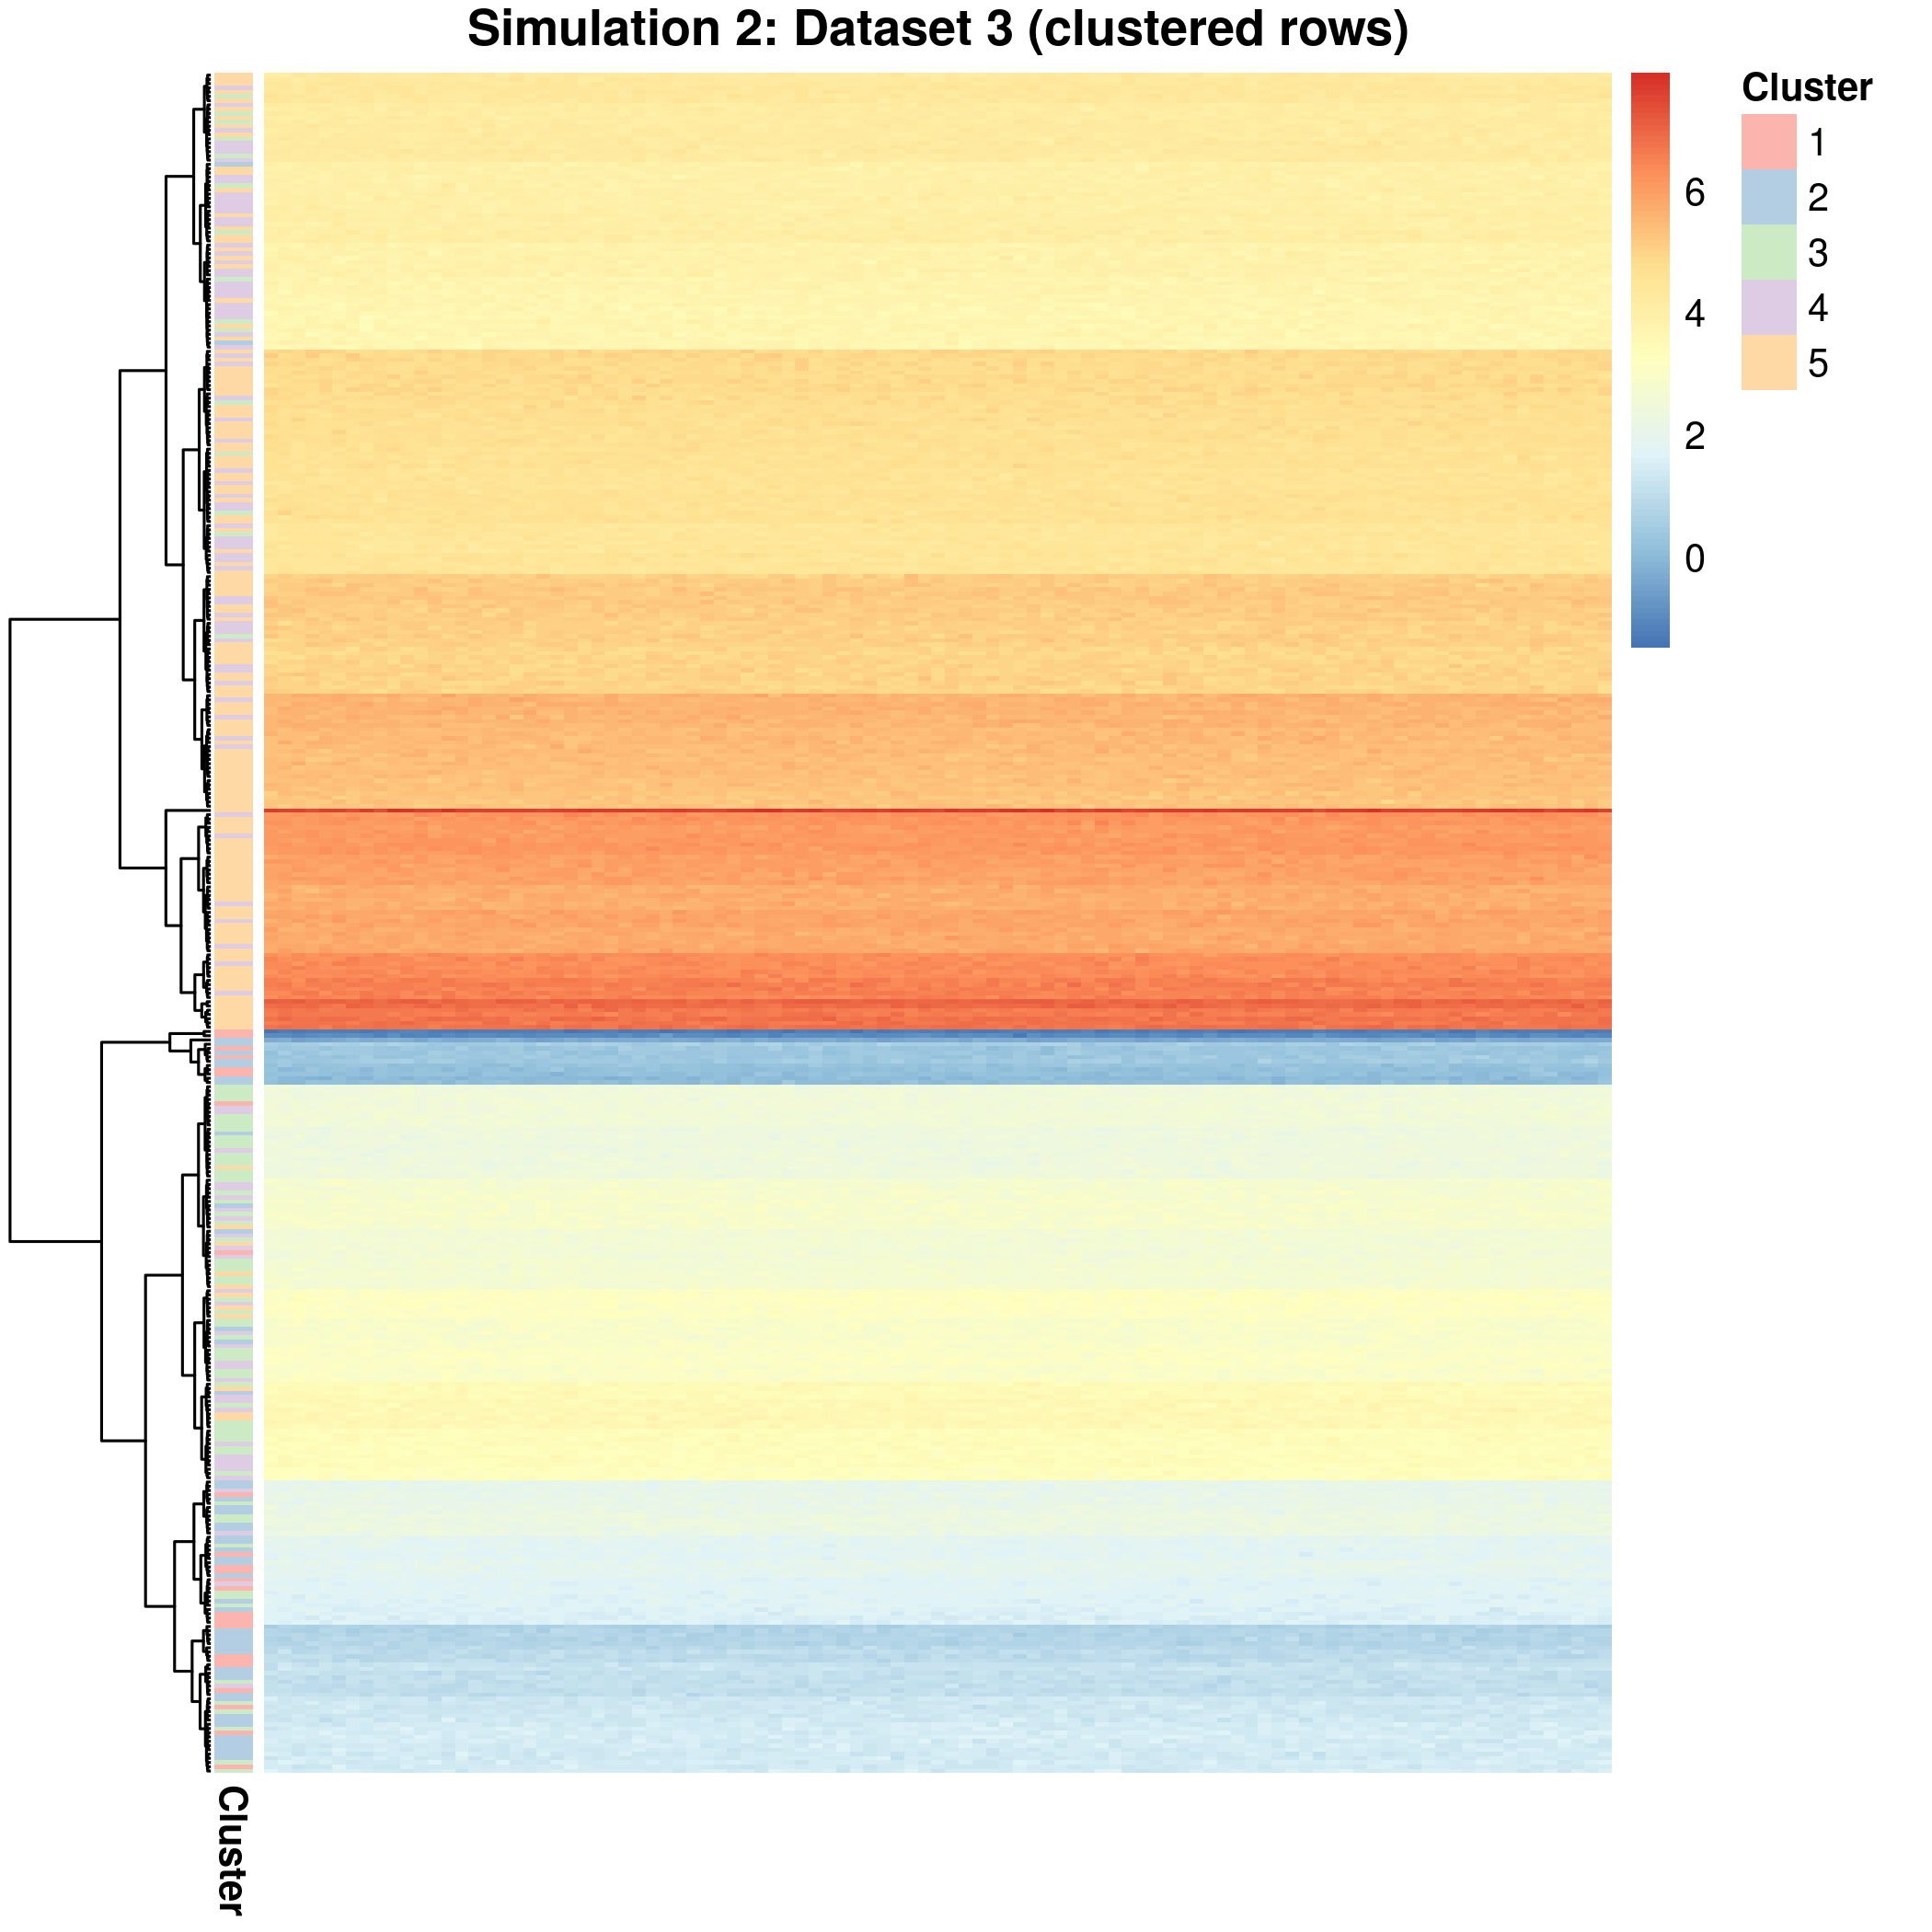
\includegraphics[scale=0.65]{Images/Gen_data/Case_2/dataset_3_clustered_rows.png}
%	\caption{Heatmap of expression data generated for the second simulation as described in section \ref{sec:sim:data:case_2} annotated by the true clustering. Note that there are 5 populations present here and that cluster membership and boundaries are not obvious.}
%	\label{fig:gen_data_3_row_ordered_sim_case_2}
%\end{figure}

	\subsubsection{Pipeline} \label{sec:simulation_pipeline}
	I run 10 separate chains of MDI for 2 million iterations with a thinning factor of 50. Secondly, consensus clustering models of 1,000 different seeds for 4 different lengths of chains ($n_{iter} = \{500, 1,000, 5,000, 10,000\}$) were applied to the same data.
	
	The estimated burn-in time required for the individual chains is checked by means of the ESS of MCMC samples drawn (see figure \ref{fig:gen_data_case_1_estimated_burn_in_plot_3}). The longest required individual burn-in is then applied to all chains to ensure a common length.
	
	After implementing the required burn-in across all chains, results are compared by various visualisations:
	
	\begin{enumerate}
		\item The chains are inspected using an autocorrelation plot and a Geweke plot to test within chain stationarity;
		\item The chains are tested for convergence across chains by means of plotting the Gelman-Rubin convergence statistic;
		\item The long chains are compared to each other and consensus clustering for various chain lengths by means of comparing the clustering at each iteration / seed to the ``ground truth" defined by the sub-populations that generated the data. Comparison is under the adjusted Rand index; and
		\item The combined space of clusterings from all the individual long chains and each version of consensus clustering are compared with the ``ground truth" using the adjusted Rand Index.
	\end{enumerate}
	
	
	\subsection{CEDAR dataset}
	I use the gene expression data from the CEDAR cohort \citep{TheInternationalIBDGeneticsConsortiumIBDriskloci2018}. This data is available in a processed form \href{http://139.165.108.18/srv/genmol/permanent/1be6993fe41c12a051c9244d67c91da2be49e5dd26a6cd79f442bc006971e2ef/crohn-index.html}{online}. This consists of 9 .csv files, one for each tissue / cell type sampled, of gene expression data for 323 individuals. These are healthy individuals of European descent; the cohort consists of 182 women and 141 men with an average age of 56 years (but ranging from 19 to 86). None of the individuals were suffering from any autoimmune or inflammatory disease and were not taking corticosteroids or non-steroid anti-inflammatory drugs (with the exception of aspirin). 
	
	With regards to tissue types, samples from five circulating immune cells types and platelets (followed in brackets by the abbreviation for the associated dataset):
	\begin{itemize}
		\item CD4+ T lymphocytes (CD4);
		\item CD8+ T lymphocytes (CD8);
		\item CD14+ monocytes (CD14);
		\item CD15+ granulocytes (CD15);
		\item CD19+ B lymphocytes (CD19); and 
		\item platelets (PLA).
	\end{itemize}
	Data from intestinal biopsies are also present, with samples taken from three distinct locations (the location of which may be seen in figure \ref{fig:colon_location}):
	\begin{itemize}
		\item the ileum (IL);
		\item the rectum (RE); and
		\item the transverse colon (TR).
	\end{itemize} 

	\begin{figure}[h]
		\centering
		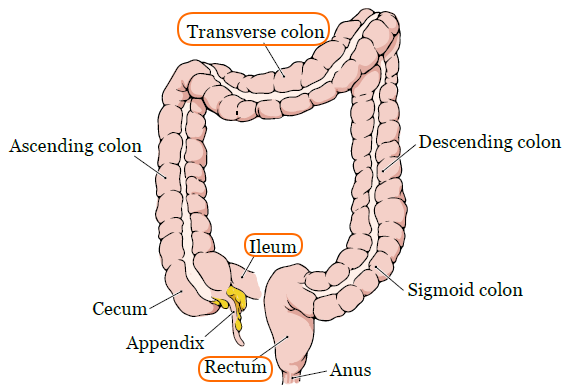
\includegraphics[scale=0.55]{Images/colon_highlight.png}
		\caption{The location of the different section of the colon and the ileum. The samples are taken from the areas with the circled names.}
		\label{fig:colon_location}
	\end{figure}
	

	Not every individual is present in every dataset (i.e. some datasets have gene expression for a different (over-lapping) set of people to other datasets). However, as genes are the object of interest this should not present a problem.
	
	Whole genome expression data were generated using HT-12 Expression BeadChips following the instructions of the manufacturer (Illumina). Each bead in the array contains a 50-mer, sequence-specific oligonucleotide probe. This allows for differential detection of signals when the BeadChips are scanned. The probes are short stretches of DNA or RNA that detect the presence of complementary sequences of nucleic acid by hybridization. The probes can then be mapped to a unique sequence which is associated with a specific gene. Note that the map from probes to genes is not 1-to-1; multiple probes can map to the same gene. The probes are uniquely labelled. This allows recognition of the probe and hence associated gene. The expression level is measured using fluorescence. Thus some samples are missing for some people as they fall below the threshold of sensitivity for which the machine is able to quantify the fluorescence within the environment in which the analysis is run.
	
	There are 18,524 probes present between the 9 datasets. It should be noted that there are differing degrees of missingness between the datasets (for instance the platelets dataset has 6,564 probes present in comparison to an average of 12,838 probes present per dataset, see figure \ref{fig:probe_presence_across_datasets}). By \emph{missingness} I mean the number of probes absent from a specific dataset that are present in at least one other dataset from the CEDAR cohort.
	
%	\begin{figure}[h]
	\begin{sidewaysfigure}
		\centering
		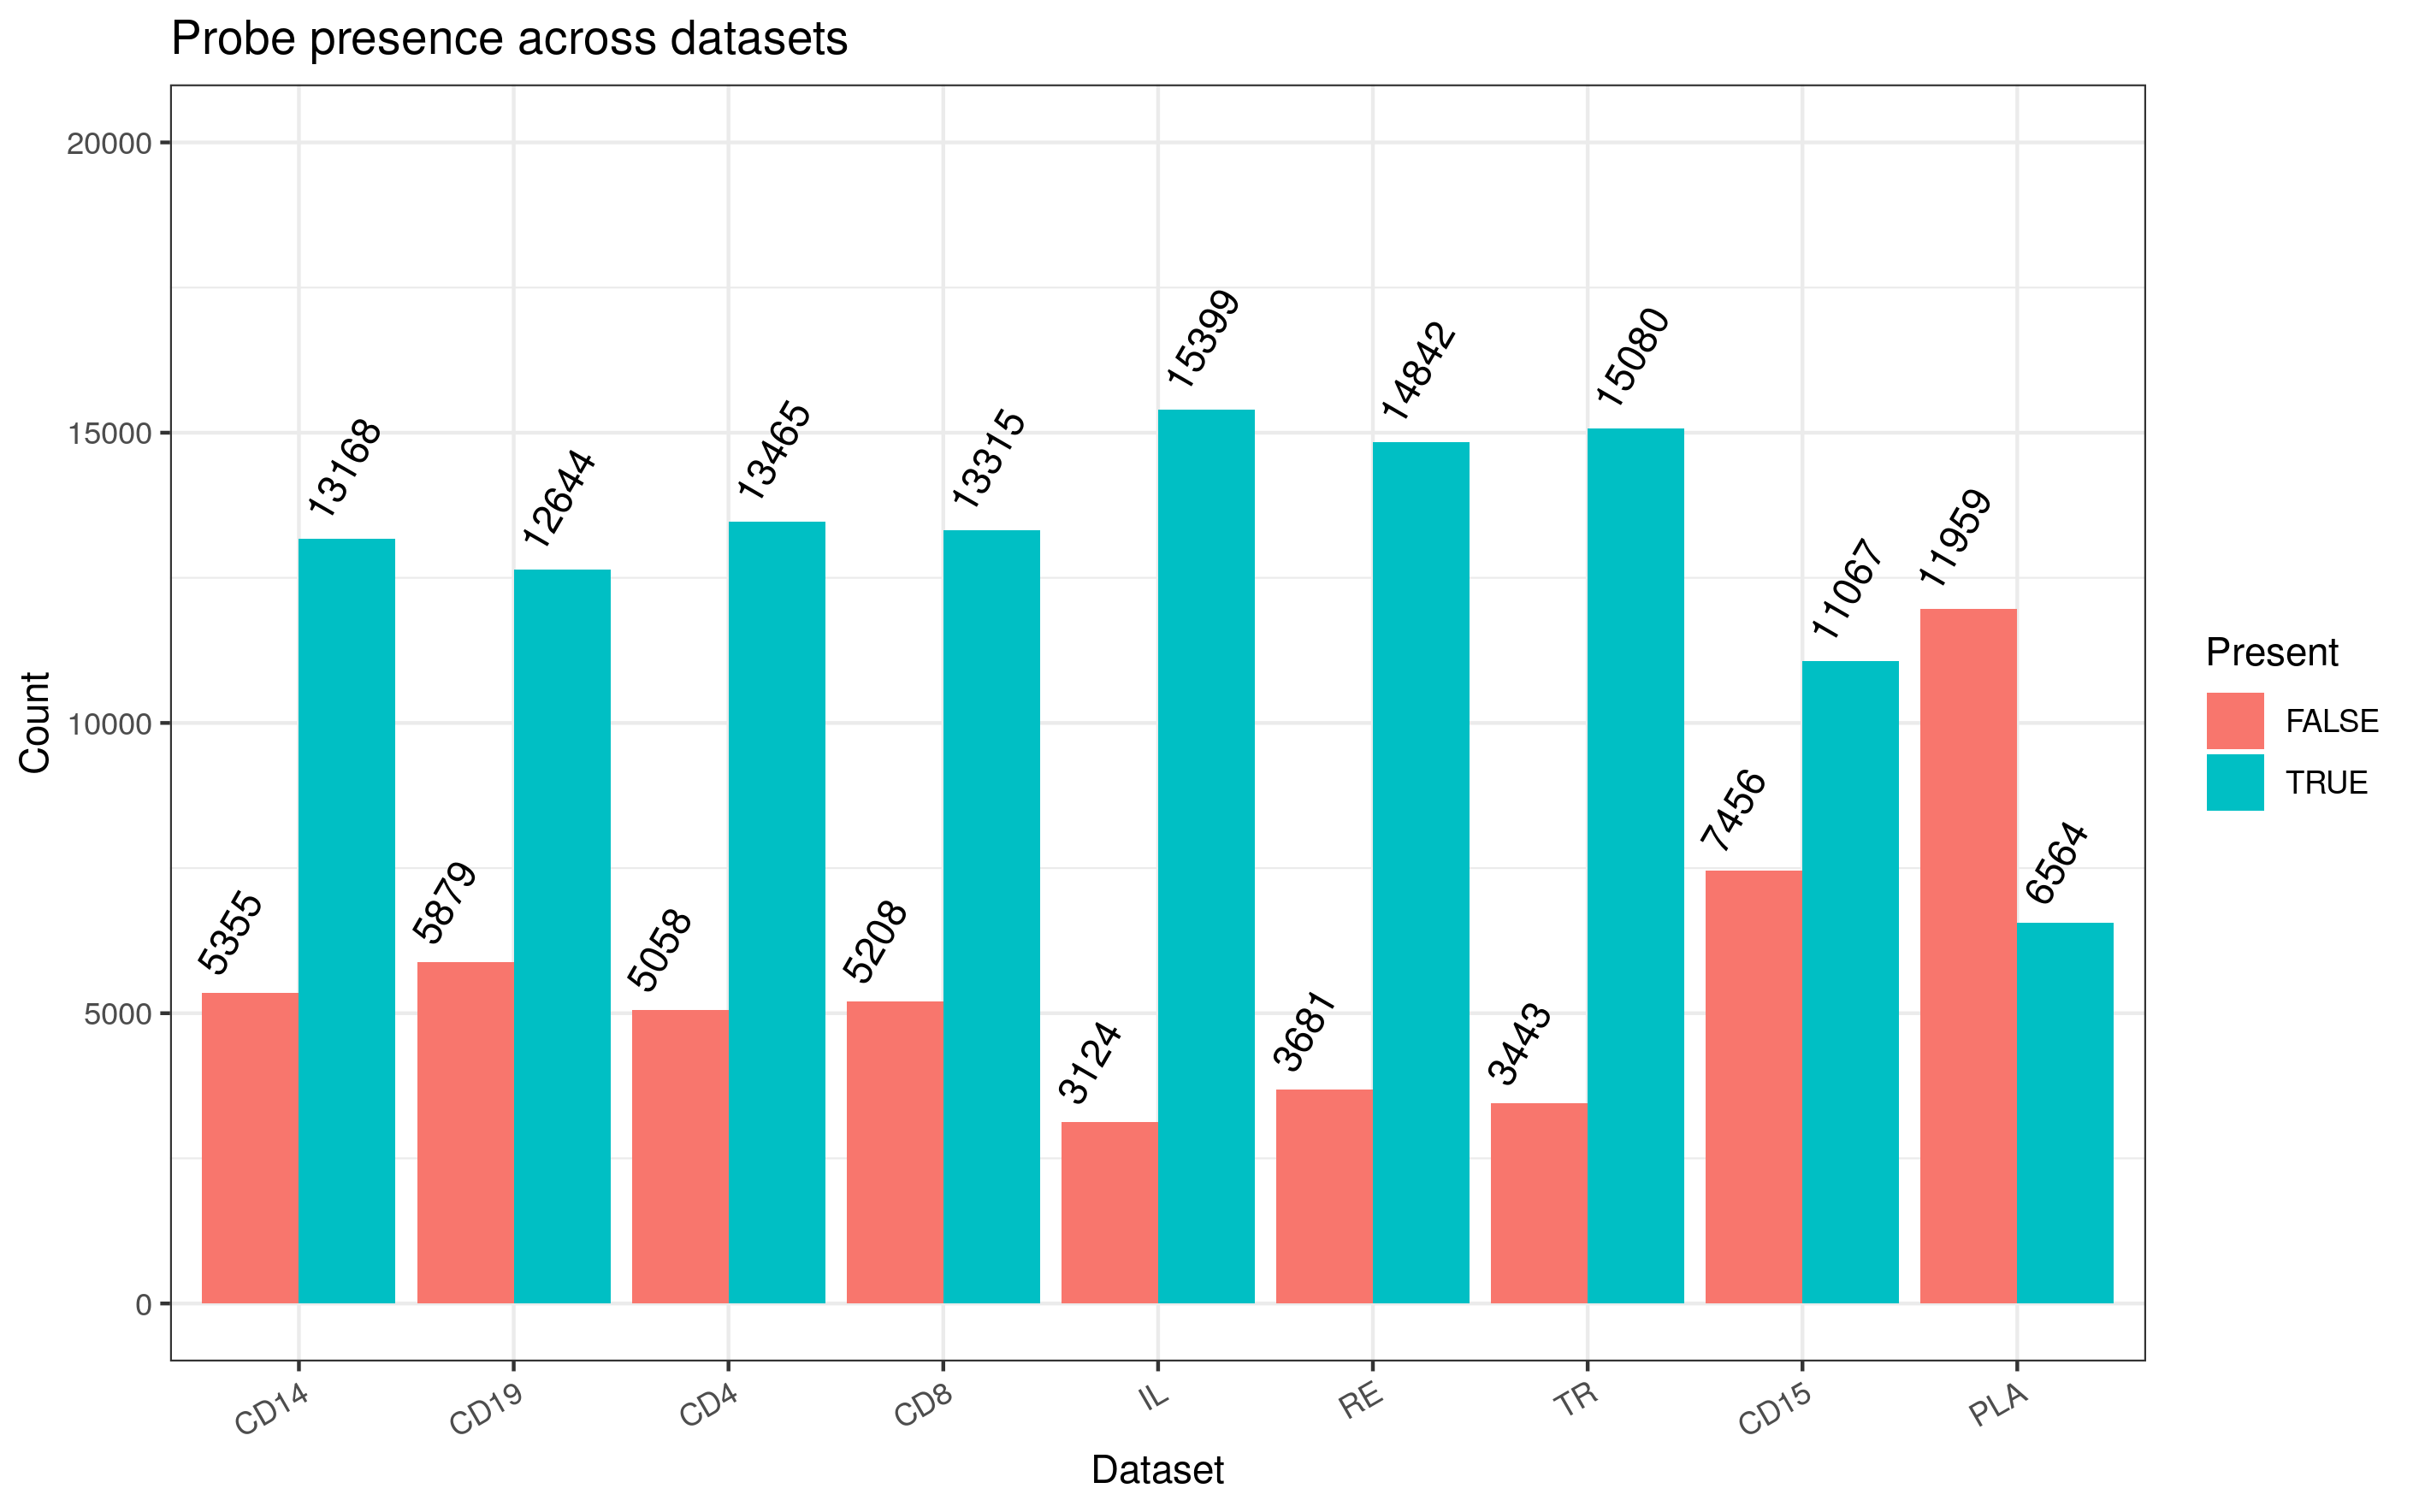
\includegraphics[scale=0.9 ]{Images/Data_inspection/probe_presence_across_datasets_no_all.png}
		\caption{Probe presence across datasets. The column on the left for each dataset records the number of probes present in at least one other dataset not present in the given dataset. The column on the right represent the number of probes for which there are observed gene expression values  in the given dataset. Note that the number of probes missing is greatest in PLA, followed by CD15.}
%			 Under ``All'' we have the number of probes present in every dataset, under ``All (excl. PLA)'' we have the number of probes present in every dataset bar PLA. Note how there is greater missingness in the PLA dataset in comparison to the others.}
		\label{fig:probe_presence_across_datasets}
	\end{sidewaysfigure}
%	\end{figure}
	
	
	Due to exponential increase in computational cost for each additional dataset, I only use the 7 most informative datasets, dropping PLA and CD15 from the analysis. From a biological perspective I expect PLA to be the least information rich as platelets have no nucleus \citep{Wrighthistogenesisbloodplatelets1910} and therefore any gene expression is an artefact from before they differentiated into platelets. With regards to CD15+ granulocytes (mast cells, basophils, neutrophils and eosinophils), these are quite distinct from B and T lymphocytes (see figure \ref{fig:white_blood_cell_differentiation}). Based on this I expect there to be less common information pertinent to clustering genes in other datasets. Arguably monocytes are equally distant, but the level of missingness in the CD15 dataset is greater than that in the CD14 dataset; thus CD15 is elimanted from my analysis.

	\begin{figure}[h]
		\centering
		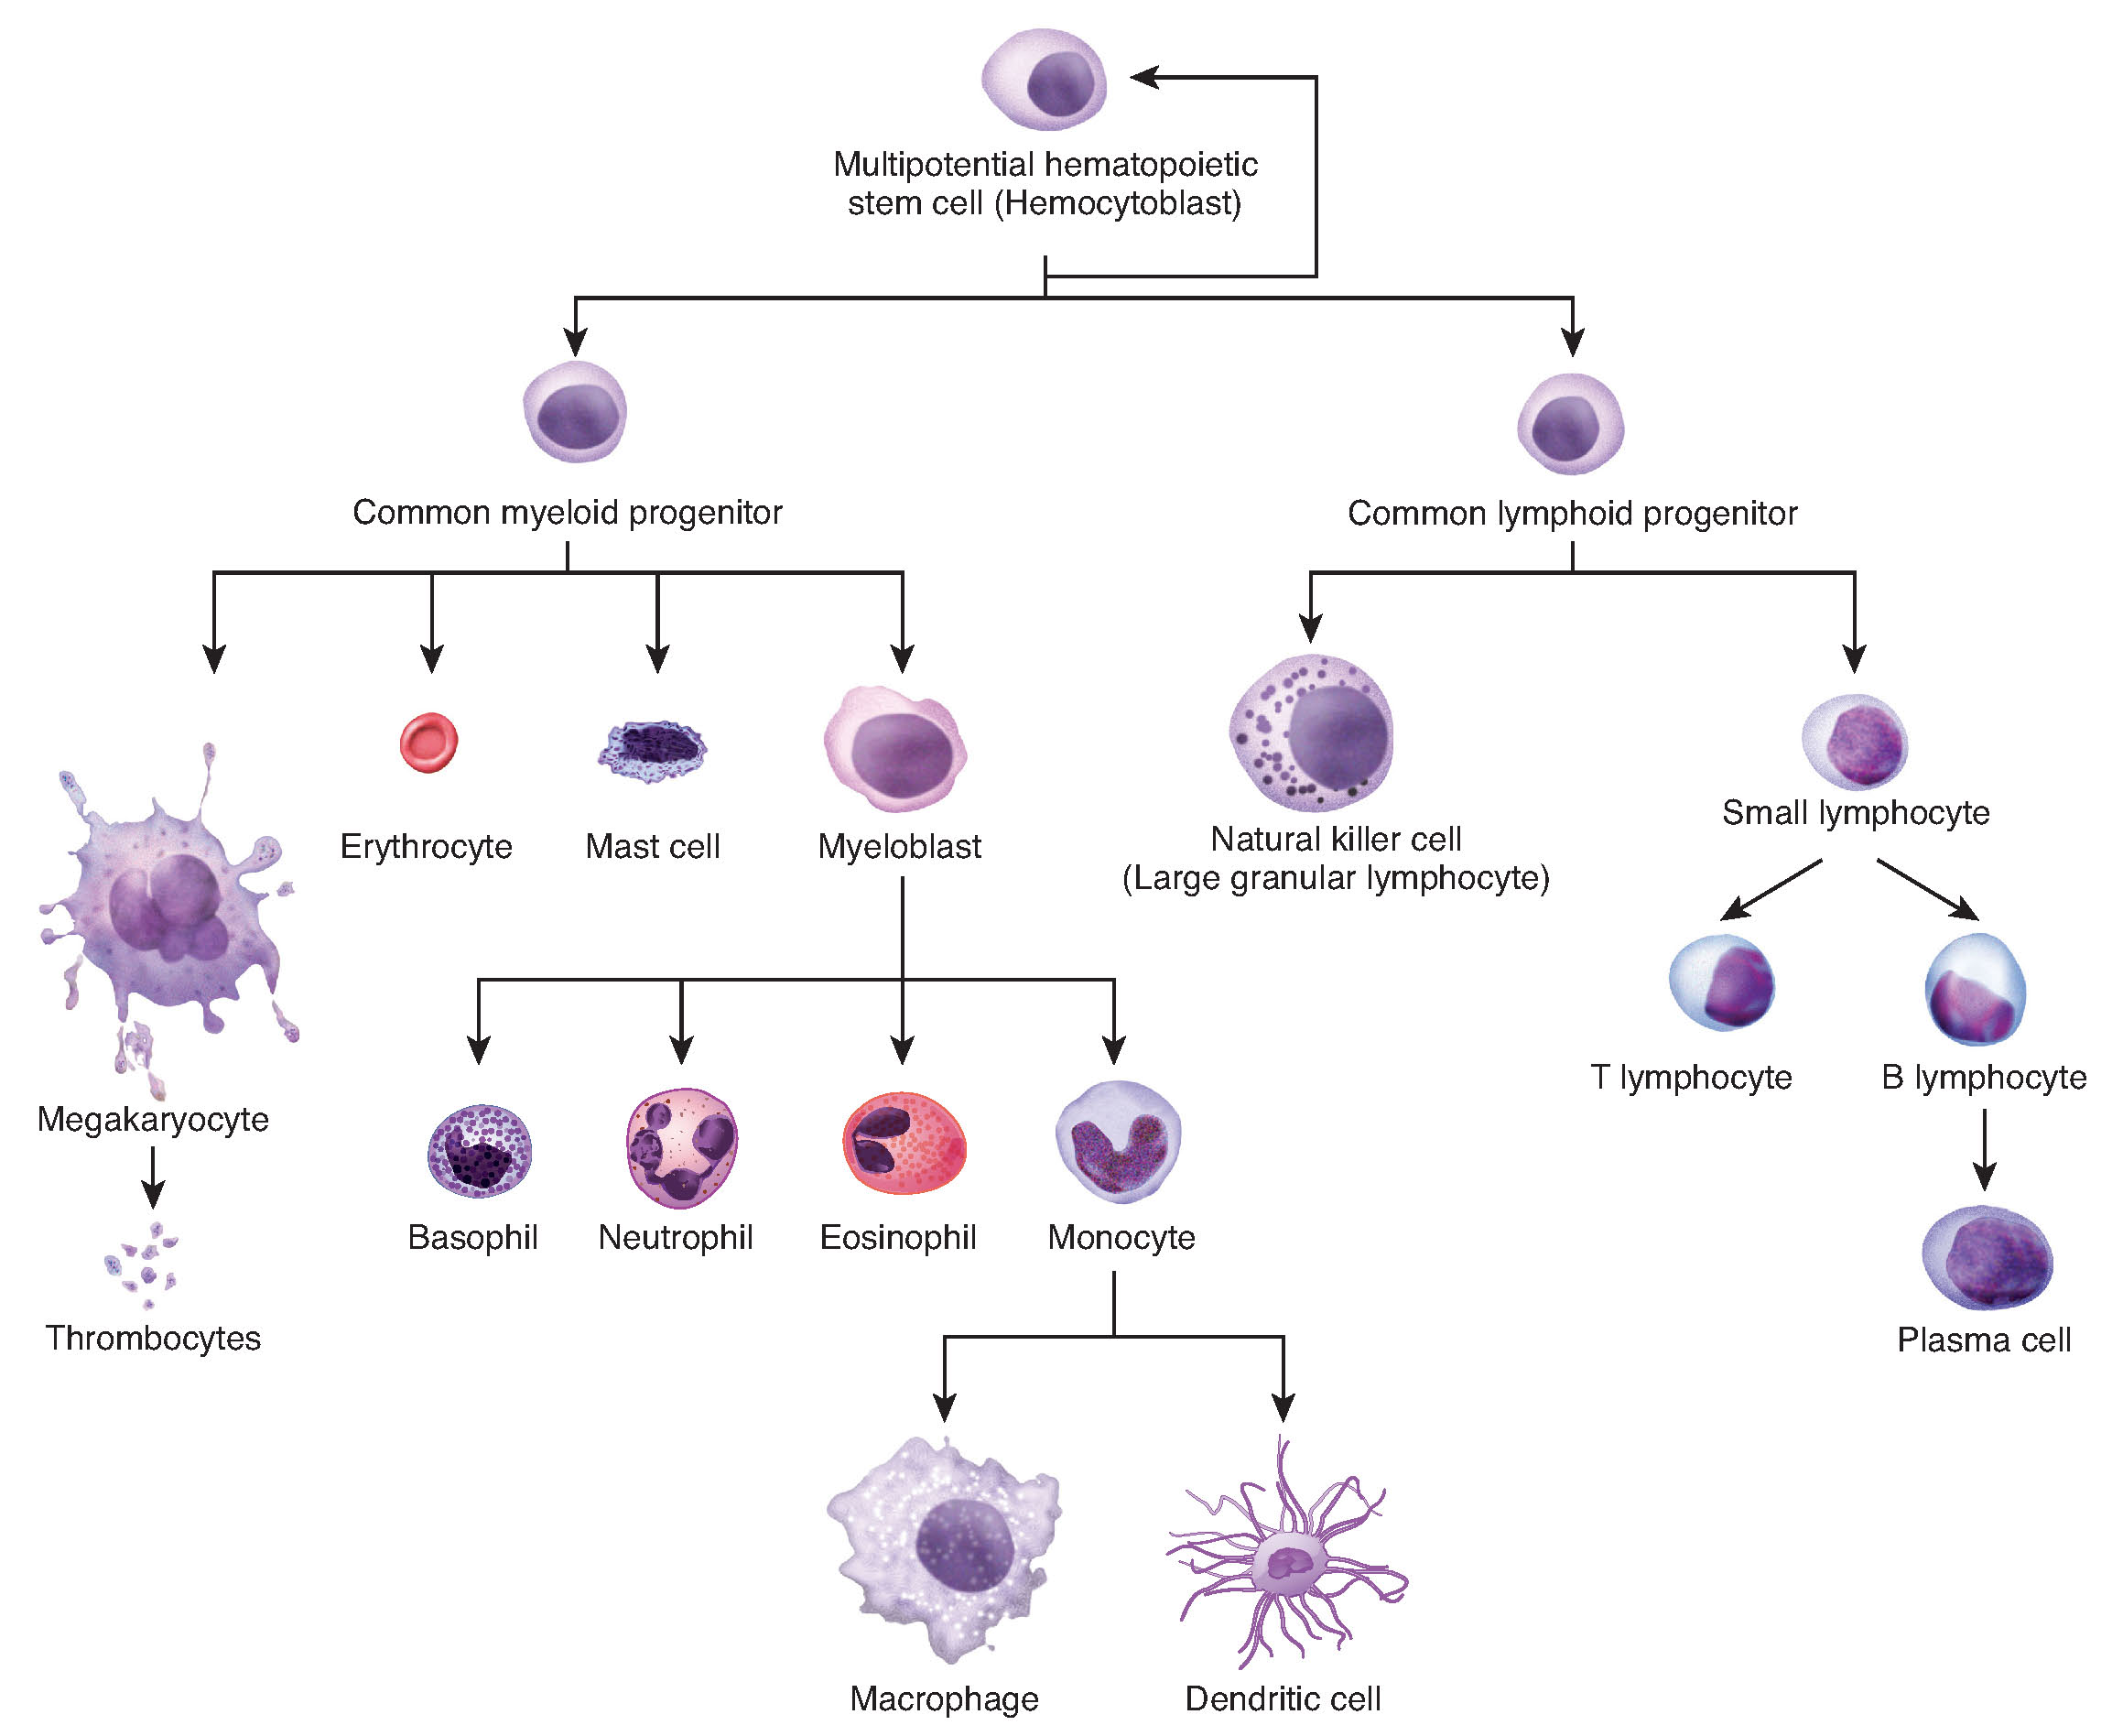
\includegraphics[scale=0.75]{Images/white_blood_cell_differentiation.jpg}
		\caption{The differentiation of multipotent cells into blood and immune cells. Image courtesy of the OpenStax project \citep{OpenStaxAnatomyPhysiology2016}.}
		\label{fig:white_blood_cell_differentiation}
	\end{figure}

	 I create two subsets of CEDAR data defined around KEGG pathways and random other probes. This is used to test if the annotated gene sets are identifiable using this method in real data. Implicit in this decision is the assumption that KEGG pathways, which are about protein interactions, can be captured by transcription data, and specifically transcription data with no repeated measurements. 
	 

	 \subsubsection{CEDAR: Case 1 - Inositol gene set} \label{sec:case_studies:cedar:dataset_1}

	I create an example dataset of 250 probes from the CEDAR dataset. This dataset contained 60 probes from the Inositol phosphate metabolism pathway as defined in the KEGG database.
	
	Inositol phosphates are molecules primarily involved in signalling processes in eukaryotes. However, specific members of the pathway are associated with a range of processes such as chromatin remodelling, mRNA export/translation and gene expression \citep{monserrate2010inositol}. The fundamental nature of this pathway means that I expect to see some structure of this pathway in each dataset; however its diversity means that there might by many sub-clusters as well as overlap with other pathways.
	
%	This scale of dataset allows implementation of MDI across 7 datasets simultaneously. 
	
	\subsubsection{CEDAR: Case 2 - 1,000 probes} \label{sec:case_studies:cedar:dataset_2}
	
	A second dataset of 1,000 probes defined by three KEGG pathways was used to explore the clustering on a larger, more diverse dataset. The pathways used are:
	
	\begin{enumerate} \label{list:kegg_pathways}
		\item Inositol phosphate metabolism (a broad biological pathway as mentioned above);
		\item NOD-like receptor signalling pathway (a specific biological pathway with known involvement in IBD \citep{CarneiroNodlikeproteinsinflammation2008, GarrettHomeostasisInflammationIntestine2010}); and
		\item Inflammatory bowel disease (IBD) (a pathological pathway).
	\end{enumerate}

	The union of these sets corresponds to 169 unique genes (or 237 probes as the mapping from the space of probes to that of genes is non-injective) that are present in the CEDAR dataset. The remaining probes are randomly selected from the total possible space (18,524 probes) less those corresponding to these genes (leaving 18,287 possible candidate probes).

 	\subsubsection{Pipeline}
	For the CEDAR data, I follow this pipeline to prepare the data for clustering. For each dataset:
	\begin{enumerate} \label{list:methods}
		\item Transpose the data to have rows associated with gene probes and columns associated with people;
		\item Remove NAs (missing observations for a probe in a person) either imputing values using the minimum expressed value of the relevant probe in the current dataset (as missingness is not random) or, if there is a large number of missing observations for a given probe or person in the dataset, removing the offending probe or person from the analysis for the dataset in question;
		\item Standardise the data (see section \ref{sec:standardisation}); and
		%		\item Apply variance stabilisation \citep{huber_variance_2002} to normalise the gene expression data;
		%		\item Inspect the data by PCA and remove outlier individuals for each dataset in each gene set;
		%	\item To apply MDI we require that each dataset have the same row names in the same order, so we re-arrange our datasets to have common order of probes;
		\item For probes entirely missing from a given dataset I generate expression from a standard normal distribution. Then these probes are expressed as noise in the dataset and any clustering imposed upon them should be due to information about these probes present in other datasets (due to the information-sharing of MDI). %; and
		%	\item Apply MDI \citep{MasonMDIGPUacceleratingintegrative2016a}.
	\end{enumerate}

	The results are generated for consensus clustering with MDI $n_{iter}=500$ and $n_{seeds}=1000$ implemented on 7 datasets. Individual mixture models were also run on each dataset for the same number of seeds and iterations as a comparison. The output was inspected under multiple lenses: 
	
	\begin{enumerate} \label{list:cedar_pipeline_analysis}
		\item The adjusted Rand index between $i^{th}$ and $1,000^{th}$ clusterings are plotted for all $i\in \{1,\ldots,1000\}$;
		\item The mean adjusted Rand index comparing clusterings across datasets are represented in a heatmap;
		\item The $\phi_{ij}$ values are plotted across seeds for all combinations of datasets;
		\item The distribution of $\phi_{ij}$ values are plotted for all combinations of datasets;
		\item The mean $\phi$ value between datasets are represented in a heatmap;
		\item The number of clusters present in any given seed are plotted for each dataset;
		\item The mass parameter for the underlying mixture models is plotted across seeds for each dataset;
		\item The PSM for each dataset is represented as a heatmap; and
		\item The comparison of the PSM, the standardised expression data and the correlation matrix were plotted with a common row ordering for each dataset. %; and
		%		\item The expression of fused genes was plotted for all dataset combinations (see an example in  figure \ref{fig:mdi_cd4_cd8_fused_genes}).
	\end{enumerate}
	Note that some of these (such as the $\phi_{ij}$ plots only apply to MDI, not the mixture models as this is the single dataset case and comparisons across datasets are not possible).
	
	The clustering for the KEGG pathways is then inspected using three visualisation techniques. For each pathway of $m$ members:
	\begin{enumerate}
		\item The annotated PSMs of the dataset and the subset of data from the pathway are plotted;
		\item I sampled $m$ random probes not in this pathway and found the mean probability of the pairwise alignment of these probes (i.e. the proportion of seeds for which any two of the $m$ probes had the same labelling). Taking $n$ (for some large $n$) of these samples allowed us to describe the distribution of the mean pairwise alignment probability and compare with the mean pairwise alignment probability of the $m$ genes from the pathway of interest; and
		\item The violin plots of the PSM entries for the pathway were compared to the PSM entries for the remaining genes in the dataset (this is not done for the 1,000 probe set as there is not sufficient granularity to tell if there is any difference).
	\end{enumerate}



%	Individuals were genotyped for more than 700,000 SNPs using Illumina's Human OmniExpress BeadChips, an iScan system and the Genome Studio software following the guidelines of the manufacturer. Variants were elimanted with call rate $\leq 0.95$, deviating from Hardy-Weinberg equilibrium $(p \leq 0.95)$, or which were monomorphic.
%	
%	Using the real genotypes of 629,570 quality-controlled autosomal SNPs as anchors, Sangar Imputation Services were used with the UK10K $+$ 1000 Genomes Phase 3 Haplotype panels to impute genotypes at autosomal variants in the population. The following were removed from the dataset indels, SNPs :
%	\begin{itemize}
%		\item with minor allele frequency (MAF) $\leq 0.05$;
%		\item deviating from Hardy-Weinberg equilibrium $(p \leq 10^{-3}$); and
%		\item with low imputation quality (INFO $\leq 0.4$).
%	\end{itemize}
%	This left $6,019,462$ high quality SNPs for eQTL analysis.
%	
%	Whole genome expression data were generated using HT-12 Expression Beadchips following the instructions of the manufacturer (Illumina). Technical outliers were removed using controls recommended by Illumina and the Lumi package
%	
%	We kept $29,464/47,323$ autosomal probes (corresponding to 19,731 genes) mapped by Re-Annotator39 to a single gene body with $\leq 2$ mismatches and not spanning known variants with MAF$>0.05$. Within cell types, we only considered probes (i.e., “usable” probes) with detection $p-value \leq 0.05$ in $\geq 25\%$ of the samples. Fluorescence intensities were $\log_2$ transformed and Robust Spline Normalized (RSN) with Lumi38.
	
	
%	\section{Methods}
%	We first show via simulated data that consensus clustering does produce similar results to a converged single run for MDI.
%	
%	We then simulate data where individual chains of MDI will struggle to converge and possibly will not converge in finite time. We show that consensus clustering explores a wider space than any individual chain and appears to describe something similar to the space described by the union of the chains.
%	
%	Finally we apply consensus clustering to 254 probes for 8 datasets from the CEDAR dataset. An initial set of probes are chosen based on the members of 3 KEGG pathways:
	
%	\begin{enumerate} \label{list:kegg_pathways}
%		\item Inositol phosphate metabolism (a broad biological pathway);
%		\item NOD-like receptor signaling pathway (a specific biological pathway with known involvement in IBD \citep{CarneiroNodlikeproteinsinflammation2008, GarrettHomeostasisInflammationIntestine2010}); and
%		\item Inflammatory bowel disease (IBD) (a pathological pathway).
%	\end{enumerate}
%	The union of these sets corresponds to 169 unique genes (or 237 probes as the mapping from the space of probes to that of genes is non-injective) that are present in the CEDAR dataset. The remaining probes are randomly selected from the total possible space (18,524 probes) less those corresponding to these genes (leaving 18,287 possible candidate probes). We then expect that the genes from the sets mentioned above (list \ref{list:kegg_pathways}) should cluster together. We use this as a test of our final clustering.
	

	
	\section{Results}
	I show the validity of my implementation of consensus clustering by means of simulations. 
	
	I show by simulation that for the inference performed by the consensus clustering method described previously:
	\begin{enumerate}
		\item It is consistent with converged MDI chains;
		\item That is is faster than running multiple long chains of MDI when a parallel environment is available;
		\item That the space sampled for possible clusterings is sensible when individual chains become trapped; and
		\item That the method is robust to different lengths of model chains.
	\end{enumerate}
	As the data is simulated, I know the true clustering as I have chosen which points are drawn from which sub-populations. I can then compare the quality of recorded clusterings generated by a single converged chain of MDI to different version of consensus clustering (i.e. varying $n_{iter}$). I let the quality of a clustering be defined by its similarity to the ground truth, measured using the \emph{adjusted Rand index} (see section \ref{sec:rand_index}).
	
	I then apply the method to real biological data with known pathways present and show encouraging results for uncovering this structure. This gene expression data is from the Correlated Expression and Disease Association Research (CEDAR) datasets. Within the CEDAR cohort there are multiple datasets containing information about the same genes for different tissues or cell types; this allows me to implement exploratory analysis of the clustering structure being tissue or cell-type dependent.
	
	\subsection{Simulations}
	\subsubsection{Case 1: Proof of consensus} \label{sec:results:case_1}
%	Using the data generated as described in section \ref{sec:sim:data:case_1}, I ran 10 separate chains of MDI for 2 million iterations with a thinning factor of 50 (this took approximately 28 hours for each chain). Secondly, consensus clustering models of 1,000 different seeds for 4 different lengths of chains were applied to the same data.
	The upper limit on the time time for each individual chain is shown in table \ref{table:results:sim_1:timing}. There is some variation across chains as some initialisations seem to reduce to fewer clusters more quickly than others (this can be seen in figure \ref{fig:gen_data_case_1_num_clusters_present_con_500}).
	
	\begin{table}[!htb] 
		\centering
		\begin{tabular}{r|c} 
			Chain length ($n_{iter}$)	& Approx. time per chain (hh:mm:ss)\\ 
			\hline
			500							& 00:02:00 \\
			1,000						& 00:03:30 \\
			5,000						& 00:10:00 \\
			10,000						& 00:20:00 \\
			2,000,000					& 28:30:00
		\end{tabular}
		\caption{Approximate time required for computation of different chain lengths of MDI for case 1 of simulations.}
		\label{table:results:sim_1:timing}
	\end{table}

	\begin{figure}[!htb]
		\centering
		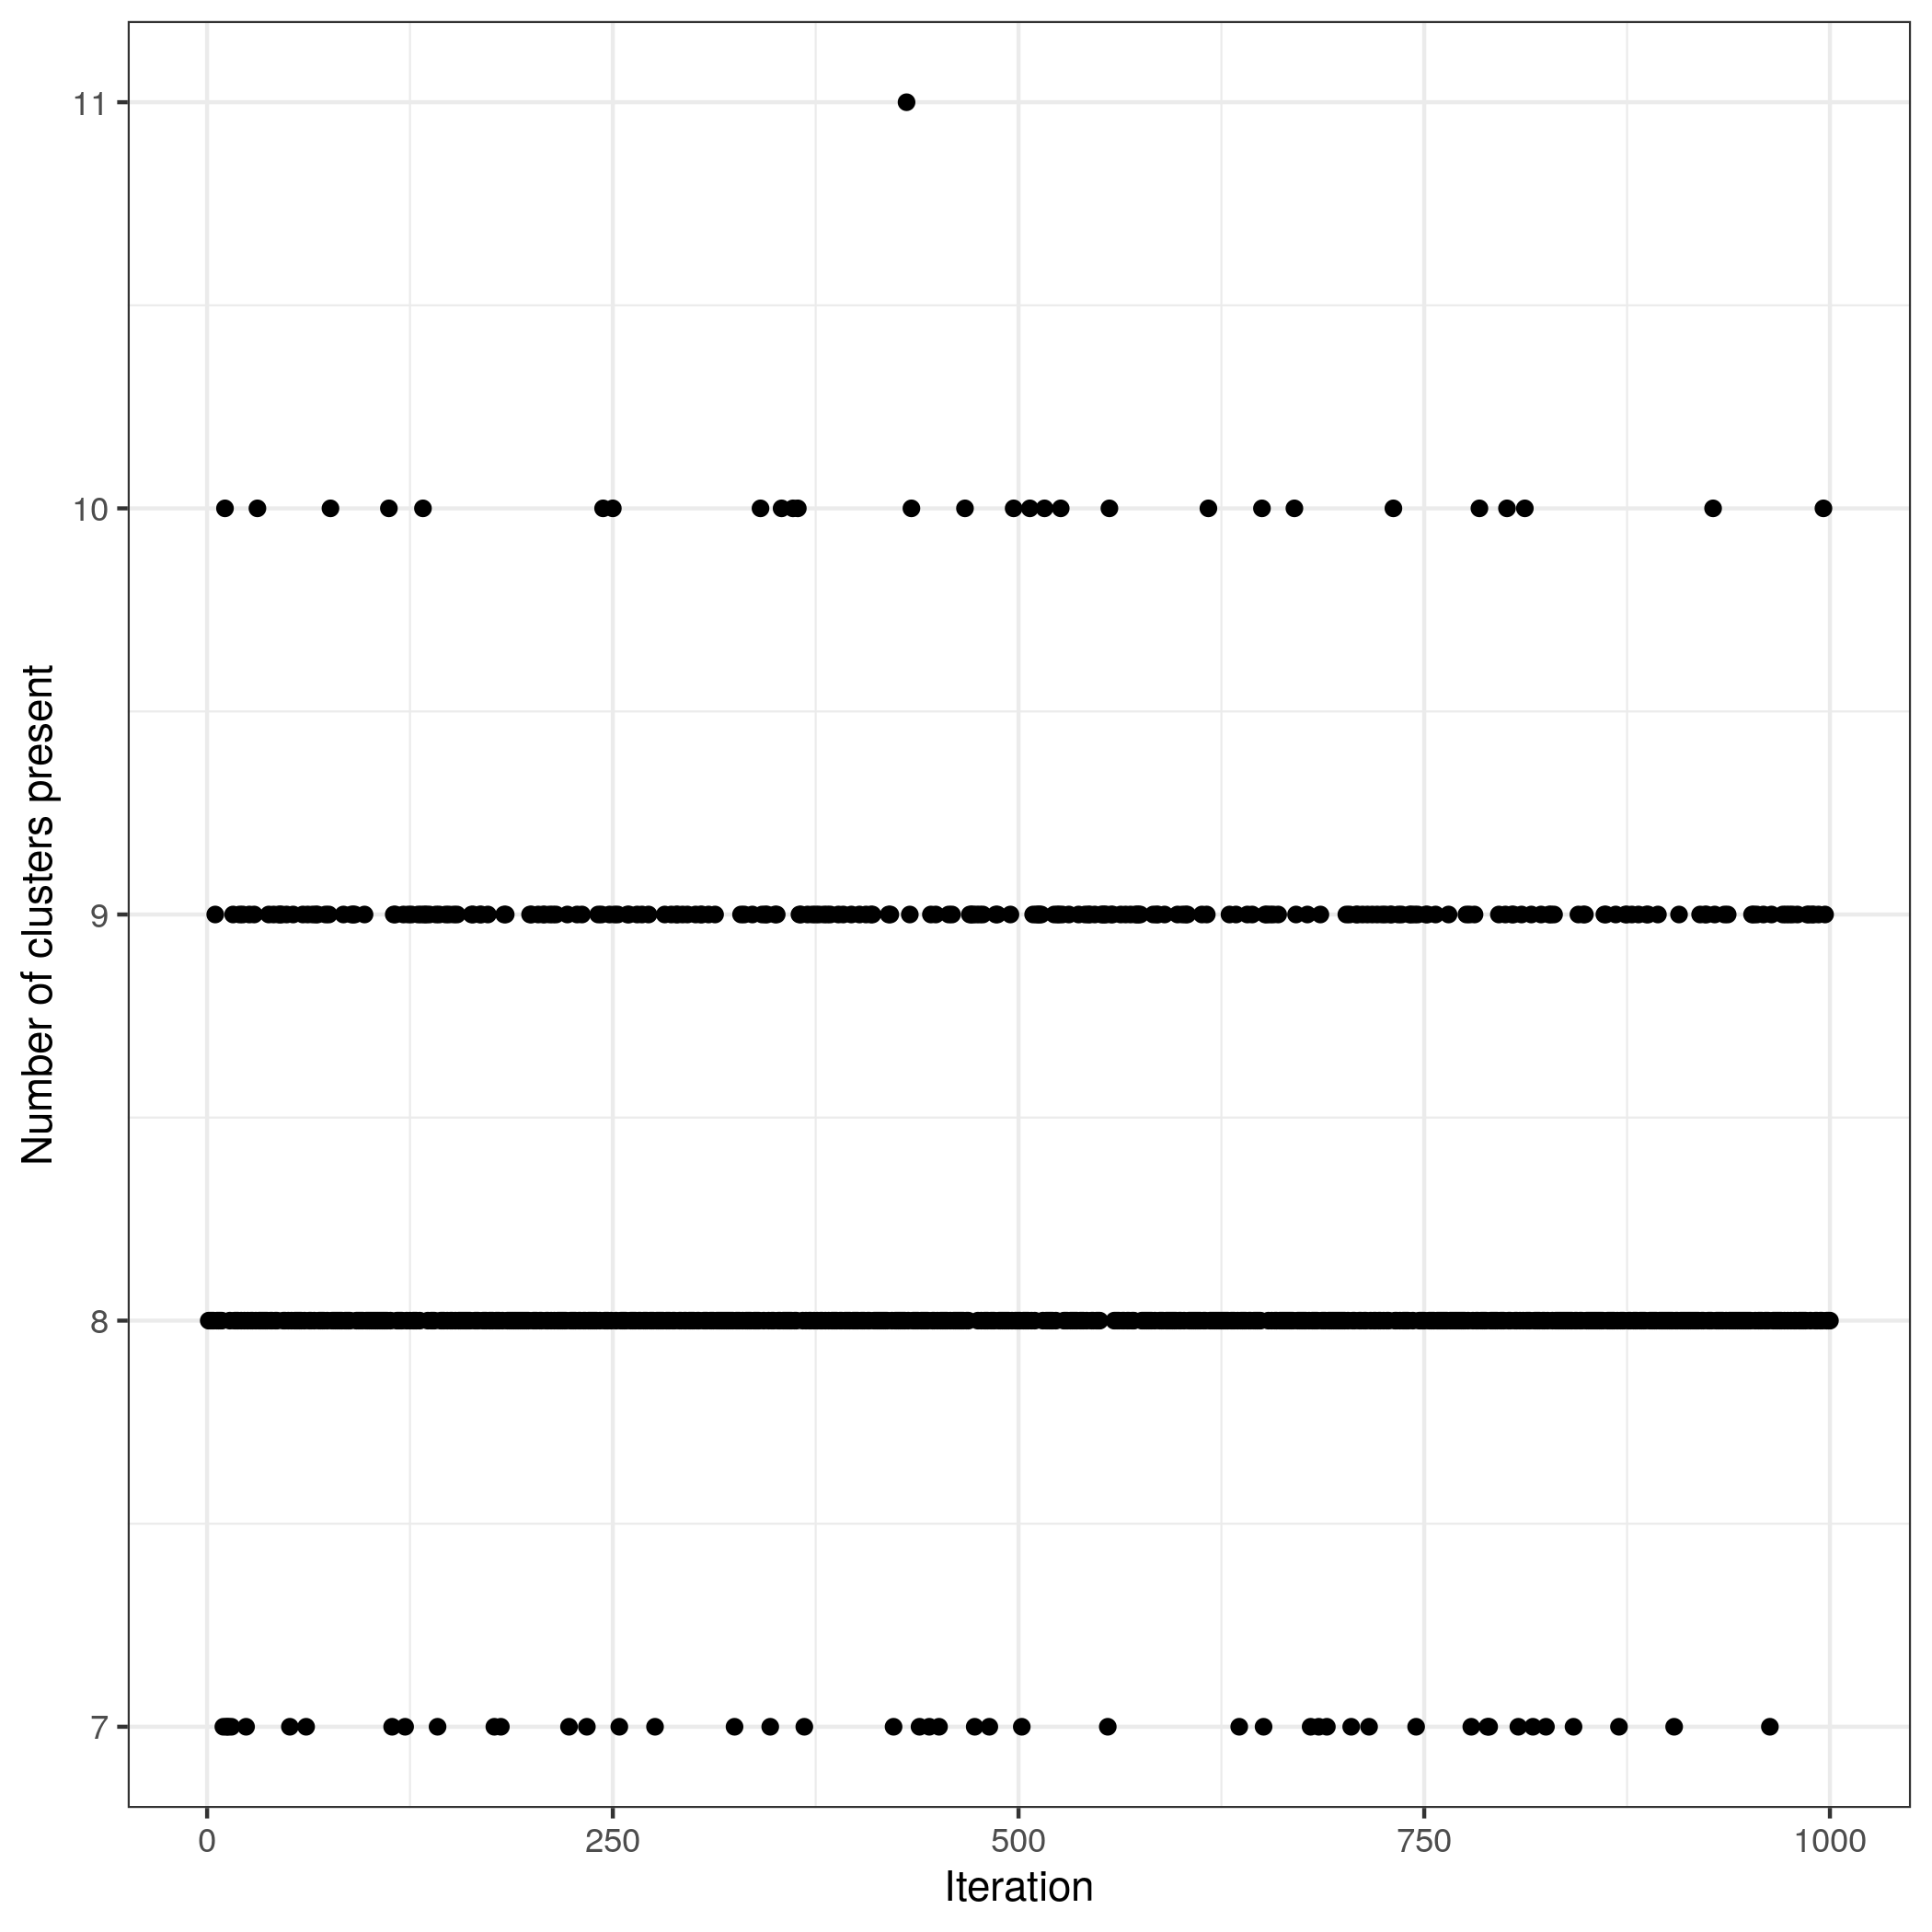
\includegraphics[scale=0.65]{Images/Gen_data/Case_1/Number_clusters_present_MDItestdata1_consensus_500.png}
		\caption{Plot of the number of clusters present in each chain of the consensus clustering for 500 iterations of MDI in dataset 1 of case 1 of the simulations. One can see that different chains reduce the number of clusters present at different rates.}
		\label{fig:gen_data_case_1_num_clusters_present_con_500}
	\end{figure}

	The estimated burn-in is 0 in this data based on figure \ref{fig:gen_data_case_1_estimated_burn_in_plot_3}, but this left one outlier clustering for each chain. Using a burn-in of 1 solved this problem and thus was implemented across all chains.
	
	\begin{enumerate}
		\item The chains were shown to have converged successfully within chain in figures \ref{fig:gen_data_case_1_autocorrelation_plot_3} and \ref{fig:gen_data_case_1_geweke_plot_3};
		\item The chains were shown to have converged across chains (see figure \ref{fig:gen_data_case_1_gelman_plot});
		\item It can be seen in figure \ref{fig:gen_data_case_1_boxplot} that individual chains of MDI outperform consensus clustering slightly in MDItestdata3, but overall perform very similarly. One can also see that consensus clustering performs similarly regardless of chain length; and
		\item In figure \ref{fig:gen_data_case_1_collapsed_boxplot}, the similarity of performance across all versions consensus clustering and the similarity to individual long chains is further highlighted.
	\end{enumerate}
	
%	The chains were shown to have converged successfully within chain, by inspecting an autocorrelation plot and a Geweke plot (see figures \ref{fig:gen_data_case_1_autocorrelation_plot_3} and \ref{fig:gen_data_case_1_geweke_plot_3}), and across chains, by means of the Gelman-Rubin convergence statistic (see figure \ref{fig:gen_data_case_1_gelman_plot}). The clustering at each iteration was compared to the clustering defined by the sub-populations that generated the data and the long chains were compared to each other and consensus clustering for various chain lengths (see figure \ref{fig:gen_data_case_1_boxplot}). One can see that the consensus clustering perform very similarly to the individual chains. Finally, in figure \ref{fig:gen_data_case_1_collapsed_boxplot}, the full space of clusterings across all chains is compared to the consensus clustering under the adjusted Rand Index.
	
%	 means of an autocorrelation plot, a Geweke plot \citep{GewekeEvaluatingAccuracySamplingBased}, a Gelman plot \citep{GelmanInferenceIterativeSimulation1992} and the distribution of adjusted Rand index comparing the clustering at each iteration (or each seed in the consensus clustering) with the clustering defined by the sub-populations used to generate the data. 


	\begin{figure}[!htb]
		\centering
		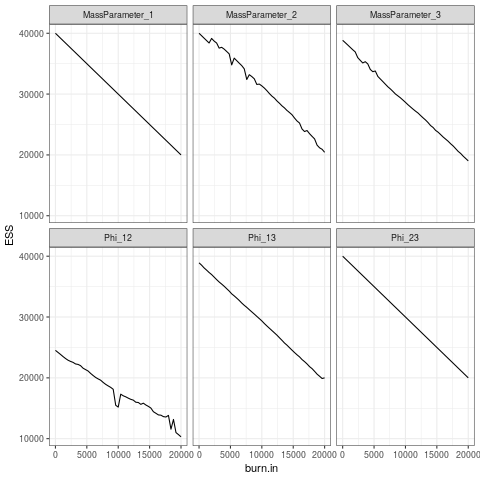
\includegraphics[scale=0.65]{Images/Gen_data/Case_1/Esimated_burn_in_plot_3.png}
		\caption{An estimate for burn-in cut-off is estimated by plotting the ESS against the burn-in at different iterations (shown here for seed 3 in case 1 of the simulations). The ESS should be maximised at the optimal estimate of the burn-in - thus one looks for the iteration at which ESS is maximised for the most parameters. Here it is a iteration 0. For a more thorough description of ESS, please go to section \ref{sec:additional_theory:sub_sec:convergence:sub_sub_sec:geweke}.}
		\label{fig:gen_data_case_1_estimated_burn_in_plot_3}
	\end{figure}


%	\newpage
	\begin{figure}[!htb]
		\centering
		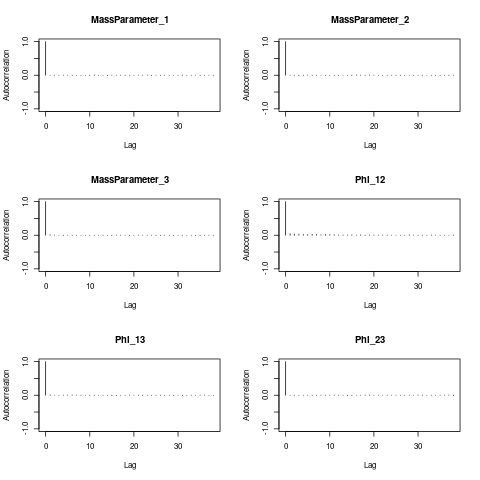
\includegraphics[scale=0.65]{Images/Gen_data/Case_1/Auto_correlation_plot_3.png}
		\caption{Autocorrelation plot for a long chain with random seed 3 in case 1 of the simulations. The autocorrelation at lag 0 is always 1 (as the observation correlates with itself). If the samples drawn are no longer correlated with samples at any lag visible here (recalling that a lag of 1 corresponds to 50 iterations due to the thinning factor) then this indicates the chain has achieved stationarity. For more discussion of autocorrelation, please read section \ref{sec:additional_theory:sub_sec:convergence:sub_sub_sec:geweke}.}
		\label{fig:gen_data_case_1_autocorrelation_plot_3}
	\end{figure}


	\begin{figure}[!htb]
		\centering
		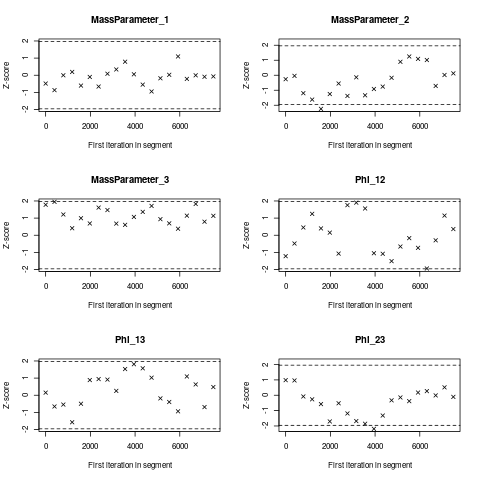
\includegraphics[scale=0.65]{Images/Gen_data/Case_1/Geweke_plot_3.png}
		\caption{Geweke plot \citep{GewekeEvaluatingAccuracySamplingBased} for a long chain with random seed 3 in case 1 of the simulations. 	This plot is generated using the plot.geweke function from the rjags R package \citep{PlummerRjags2018}. If the chain has reached stationarity the Z-scores should be described by a standard normal distribution. This means that 95\% of the  values should be contained within the dashed lines as is the case here. This indicates, particularly in conjunction with figure \ref{fig:gen_data_case_1_autocorrelation_plot_3}, that the chain has converged. For more information, please see section \ref{sec:additional_theory:sub_sec:convergence:sub_sub_sec:geweke}.}
			
%		The samples are split into disjoint bins, with the first set of $\frac{n}{2(n_{bins} -1)}$ samples in the first bin, the second set of $\frac{n}{2(n_{bins} -1)}$ samples in the second, etc. with the final bin containing the final $50\%$ of samples. Geweke's $Z$-score \citep{GewekeEvaluatingAccuracySamplingBased} is repeatedly calculated, comparing the members of each bin to the final $50\%$ of samples with the $Z$-scores than plotted as above. }
		\label{fig:gen_data_case_1_geweke_plot_3}
	\end{figure}
		
%	\newpage
	
	\begin{figure}[!htb]
			\centering
			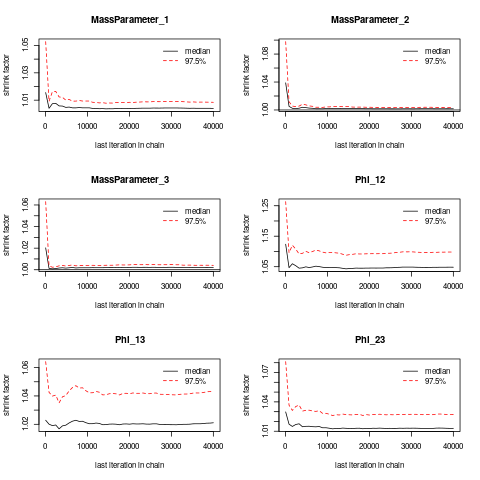
\includegraphics[scale=0.65]{Images/Gen_data/Case_1/Gelman_plot.png}
			\caption{Plot of the shrink factor described by \citet{GelmanInferenceIterativeSimulation1992} for the continuous variables across chains in case 1 of the simulations. If the chains are converged (and thus describing similar spaces to one another) the values should tend to 1 (as is the case here). For a more thorough description of the shrink factor, please see section \ref{sec:additional_theory:sub_sec:convergence:sub_sub_sec:gelman}.}
			\label{fig:gen_data_case_1_gelman_plot}
		\end{figure}

%	\newpage
	
%	\begin{figure}[h]
		\begin{sidewaysfigure}
			\centering
			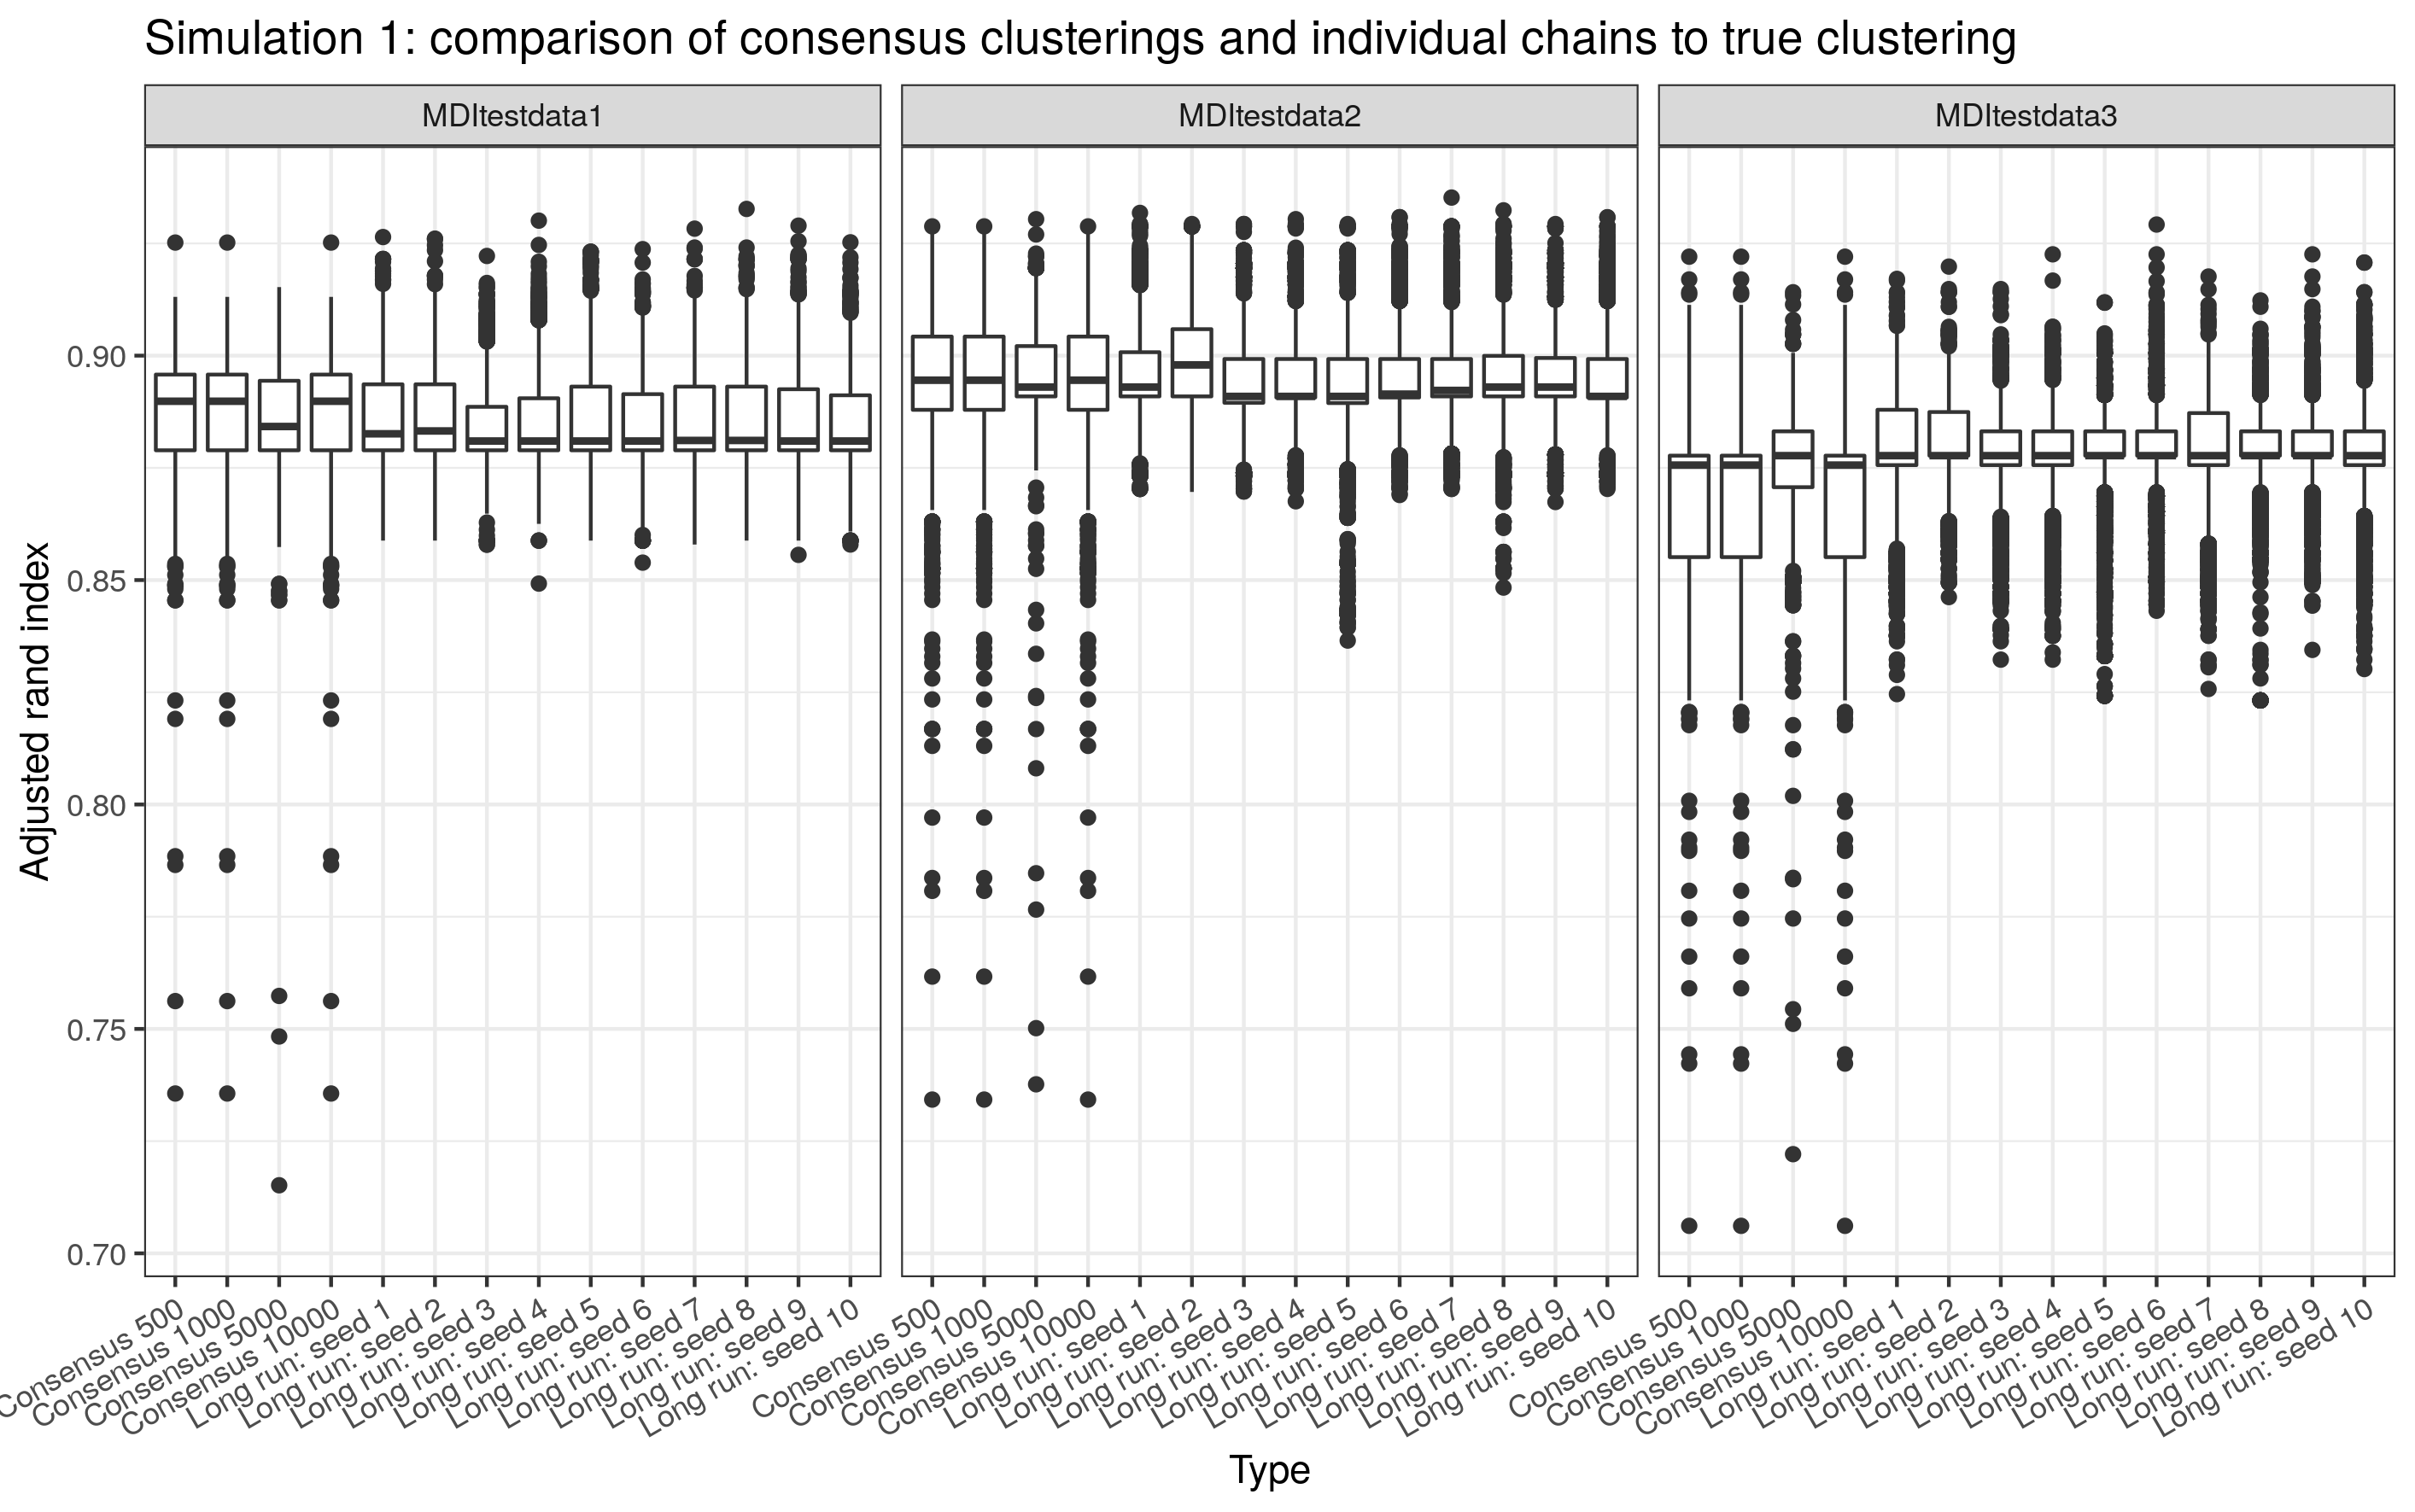
\includegraphics[scale=0.9]{Images/Gen_data/Case_1/box_plot_ari_true_clustering_burn_in.png}
			\caption{Box plots for distribution of adjusted rand index between the clustering at each iteration to the true clustering for different lengths of consensus clustering and different initialisation of long chains for case 1 of the simulations. The consensus clustering results are consistent across chain length. There is some evidence (more obvious when combined with figure \ref{fig:gen_data_case_1_collapsed_boxplot}) that individual chains of MDI performs marginally better. However, as this data is based upon some designed for MDI to perform optimally and as the results largely overlap I do not think the difference in performance is significant. Consensus clustering can have some chains that perform more poorly, but note that the y-axis does not have a large range, so this can be misleading, and even then the majority of samples are high-performing.}
			\label{fig:gen_data_case_1_boxplot}
		\end{sidewaysfigure}
		%	\end{figure}
		
%		\newpage
		
		\begin{figure}[!htb]
			\centering
			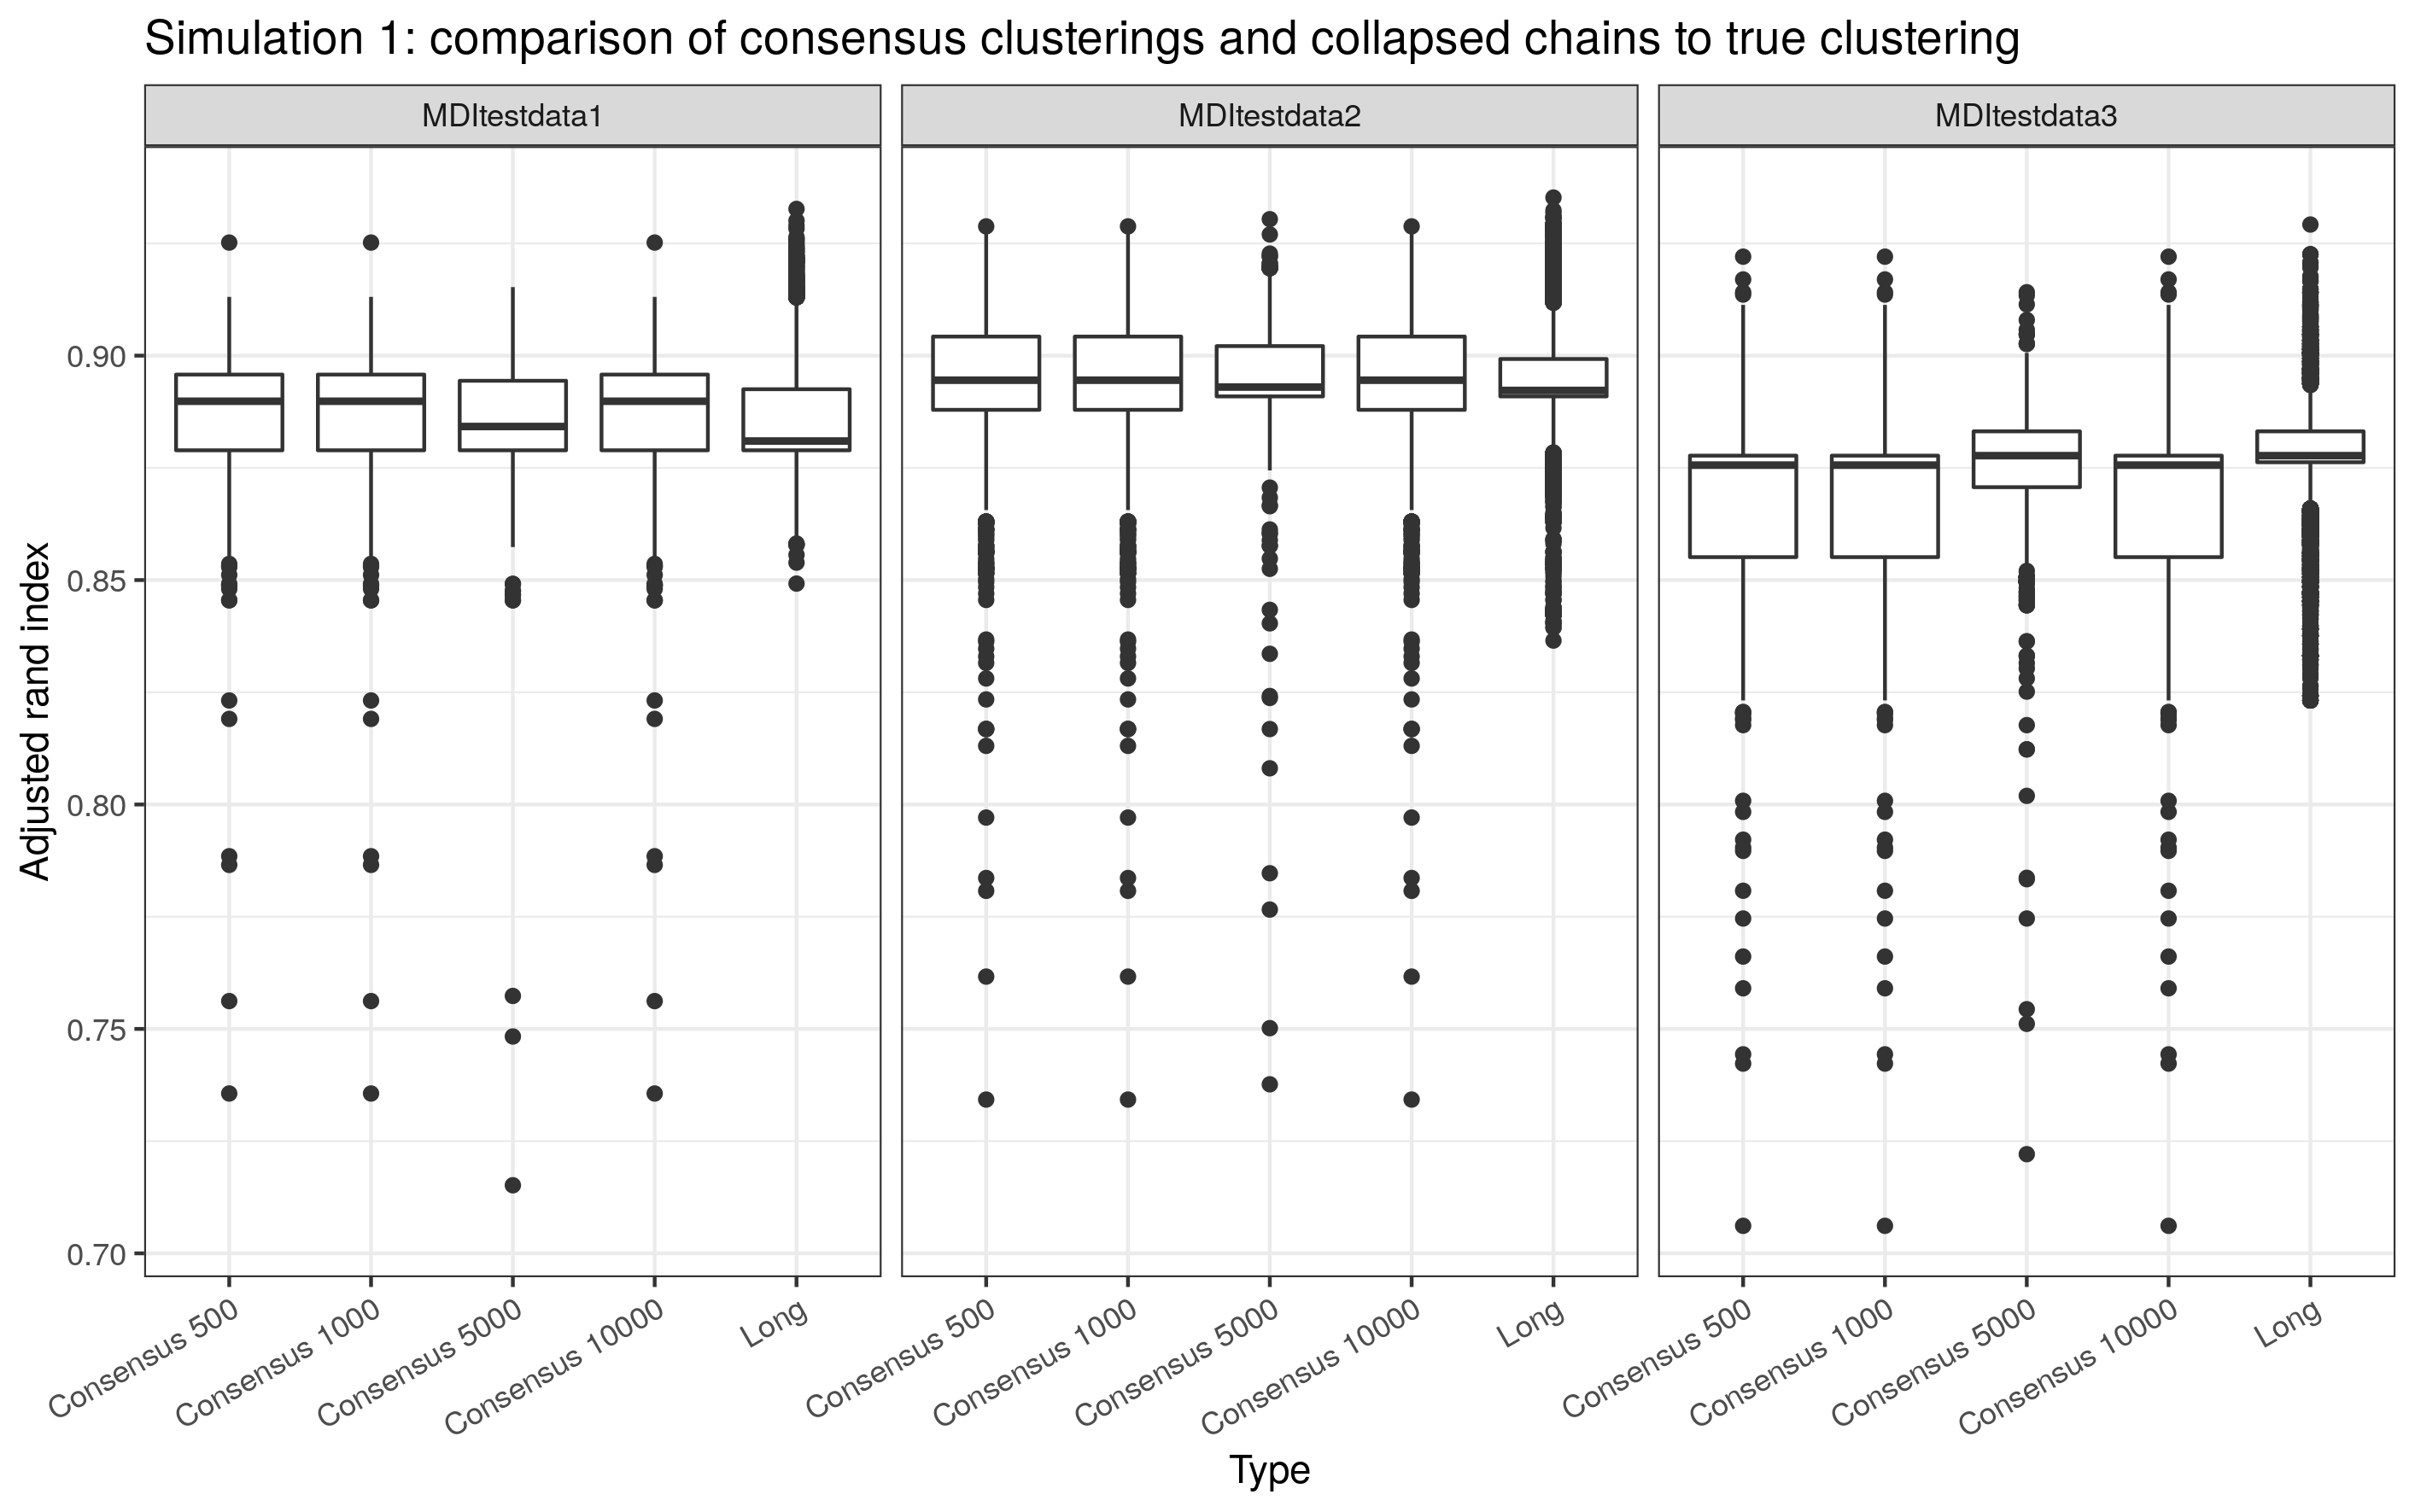
\includegraphics[scale=0.65]{Images/Gen_data/Case_1/box_plot_ari_true_clustering_collapsed_long_burn_in.png}
			\caption{Box plots for distribution of adjusted rand index between the clustering at each iteration to the true clustering for different lengths of consensus clustering and the collapsed long chains for case 1 of the simulations. One can see that in MDItestdata3 the long chains are outperforming the consensus clusterings (for most cases), but that for the other datasets there is more overlap.}
			\label{fig:gen_data_case_1_collapsed_boxplot}
		\end{figure}
		
%		\newpage

	
	\subsubsection{Case 2: Overcoming multiple modes} \label{sec:results:case_2}
%	Similar versions of consensus clustering and individual chains were run for the data generated as described in section \ref{sec:sim:data:case_2}. These were then compared using the same methods as for section \ref{sec:results:case_1}. 
	
	The burn-in required by the slowest converging chain was 20,000 recorded samples. This was applied to each chain before investigating convergence, but I include an example (figure \ref{fig:gen_data_case_2_bad_autocorrelation_plot_burn_20000_9}) of the auto-correlation prior to applying the burn-in. One can see an example in both figures \ref{fig:gen_data_case_2_autocorrelation_plot_burn_20000_1} and \ref{fig:gen_data_case_2_geweke_plot_1} that indicates the individual chain has reached stationarity (the individual chain is no longer exploring new space). However, convergence has not been achieved across chains as is shown in figure \ref{fig:gen_data_case_2_gelman_plot}. The space explored across the ten chains is compared to that explored in each of the consensus clusterings (see figures \ref{fig:gen_data_case_2_boxplot}, \ref{fig:gen_data_case_2_collapsed_boxplot} and \ref{fig:gen_data_case_2_collapsed_violin_plot}). It can be seen that each version of consensus clustering performs similarly to each other and furthermore that they perform similarly to the union of the long MDI chains.
	
%			\newpage
	
	\begin{figure}[!htb]
		\centering
		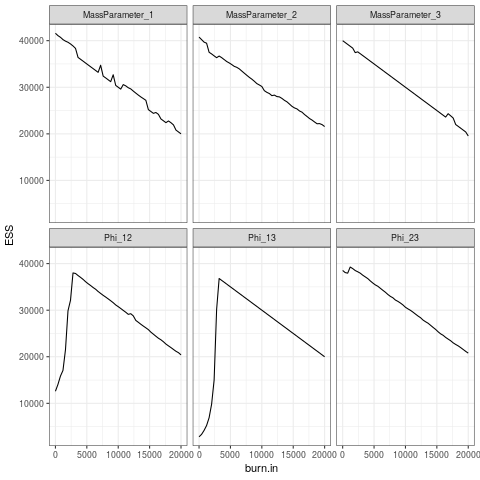
\includegraphics[scale=0.65]{Images/Gen_data/Case_2/Esimated_burn_in_plot_1.png}
		\caption{Plot of ESS against burn-in at different iterations for a long chain with random seed 1 in case 2 of the simulations.}
		\label{fig:gen_data_case_2_estimated_burn_in_plot_1}
	\end{figure}
	
	\begin{figure}[!htb]
		\centering
		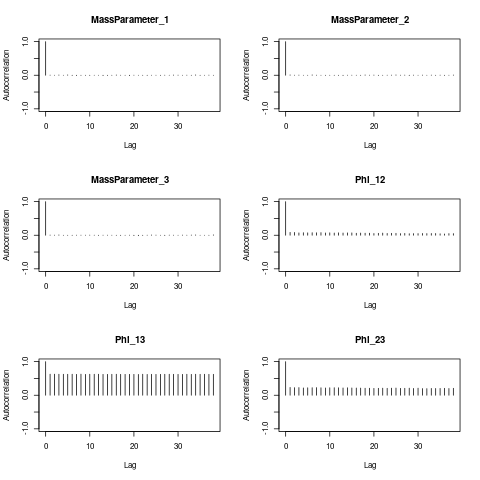
\includegraphics[scale=0.65]{Images/Gen_data/Case_2/Auto_correlation_plot_9.png}
		\caption{Autocorrelation plot for a long chain with no burn-in. The high lag present for Phi\_13 indicates that the chain has not achieved stationarity.}
		\label{fig:gen_data_case_2_bad_autocorrelation_plot_burn_20000_9}
	\end{figure}
	
	
	%	\newpage
	\begin{figure}[!htb]
		\centering
		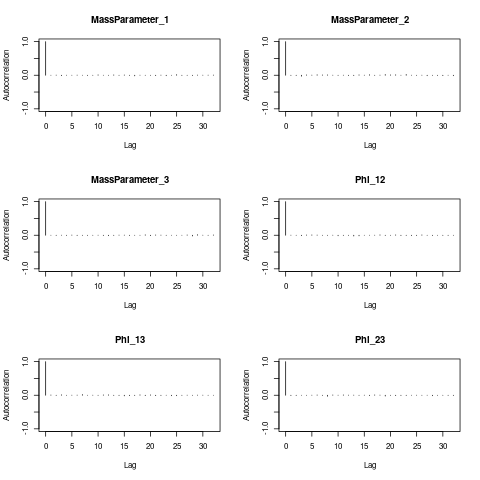
\includegraphics[scale=0.65]{Images/Gen_data/Case_2/Auto_correlation_plot_burn_20000_1.png}
		\caption{Autocorrelation plot for a long chain with random seed 1 in case 2 of the simulations after a burn-in of 20,000 samples. This result is indicative of stationarity within a chain (low lag values).}
		\label{fig:gen_data_case_2_autocorrelation_plot_burn_20000_1}
	\end{figure}
	
	
	\begin{figure}[!htb]
			\centering
			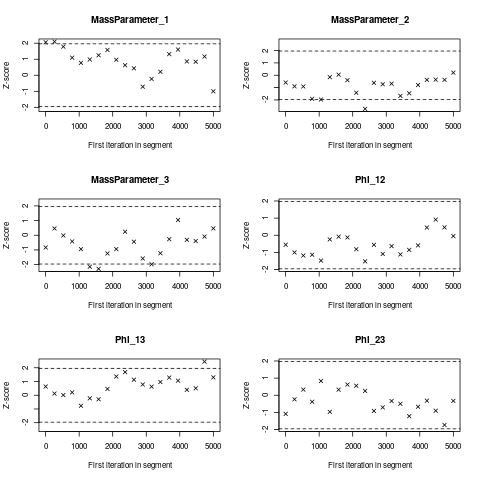
\includegraphics[scale=0.65]{Images/Gen_data/Case_2/Geweke_plot_burn_20000_1.png}
			\caption{Geweke plot for a long chain with random seed 1 in case 2 of the simulations. $95\%$ of the points are between the dashed lines, indicating stationarity within the chain.}
			\label{fig:gen_data_case_2_geweke_plot_1}
		\end{figure}
		
%	\newpage
	
	\begin{figure}[!htb]
			\centering
			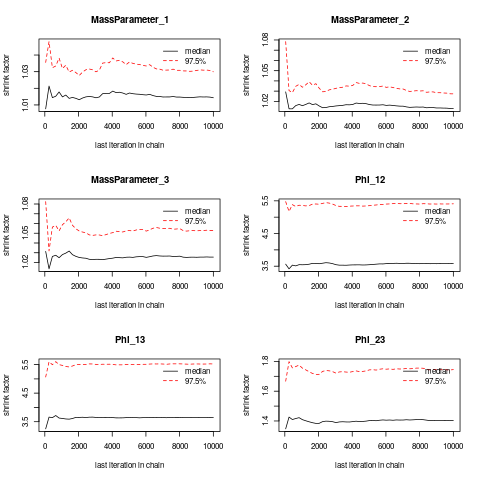
\includegraphics[scale=0.65]{Images/Gen_data/Case_2/Gelman_plot_burn_20000.png}
			\caption{Plot of the  Gelman-Rubin shrink factor for the continuous variables across chains in case 2 of the simulations. The behaviour of the shrink factor for the $\phi_{ij}$ parameters indicates that convergence across chains has not been achieved.}
			\label{fig:gen_data_case_2_gelman_plot}
		\end{figure}
	
%		\newpage
	
%	\begin{figure}[h]
		\begin{sidewaysfigure}[!htb]
		\centering
		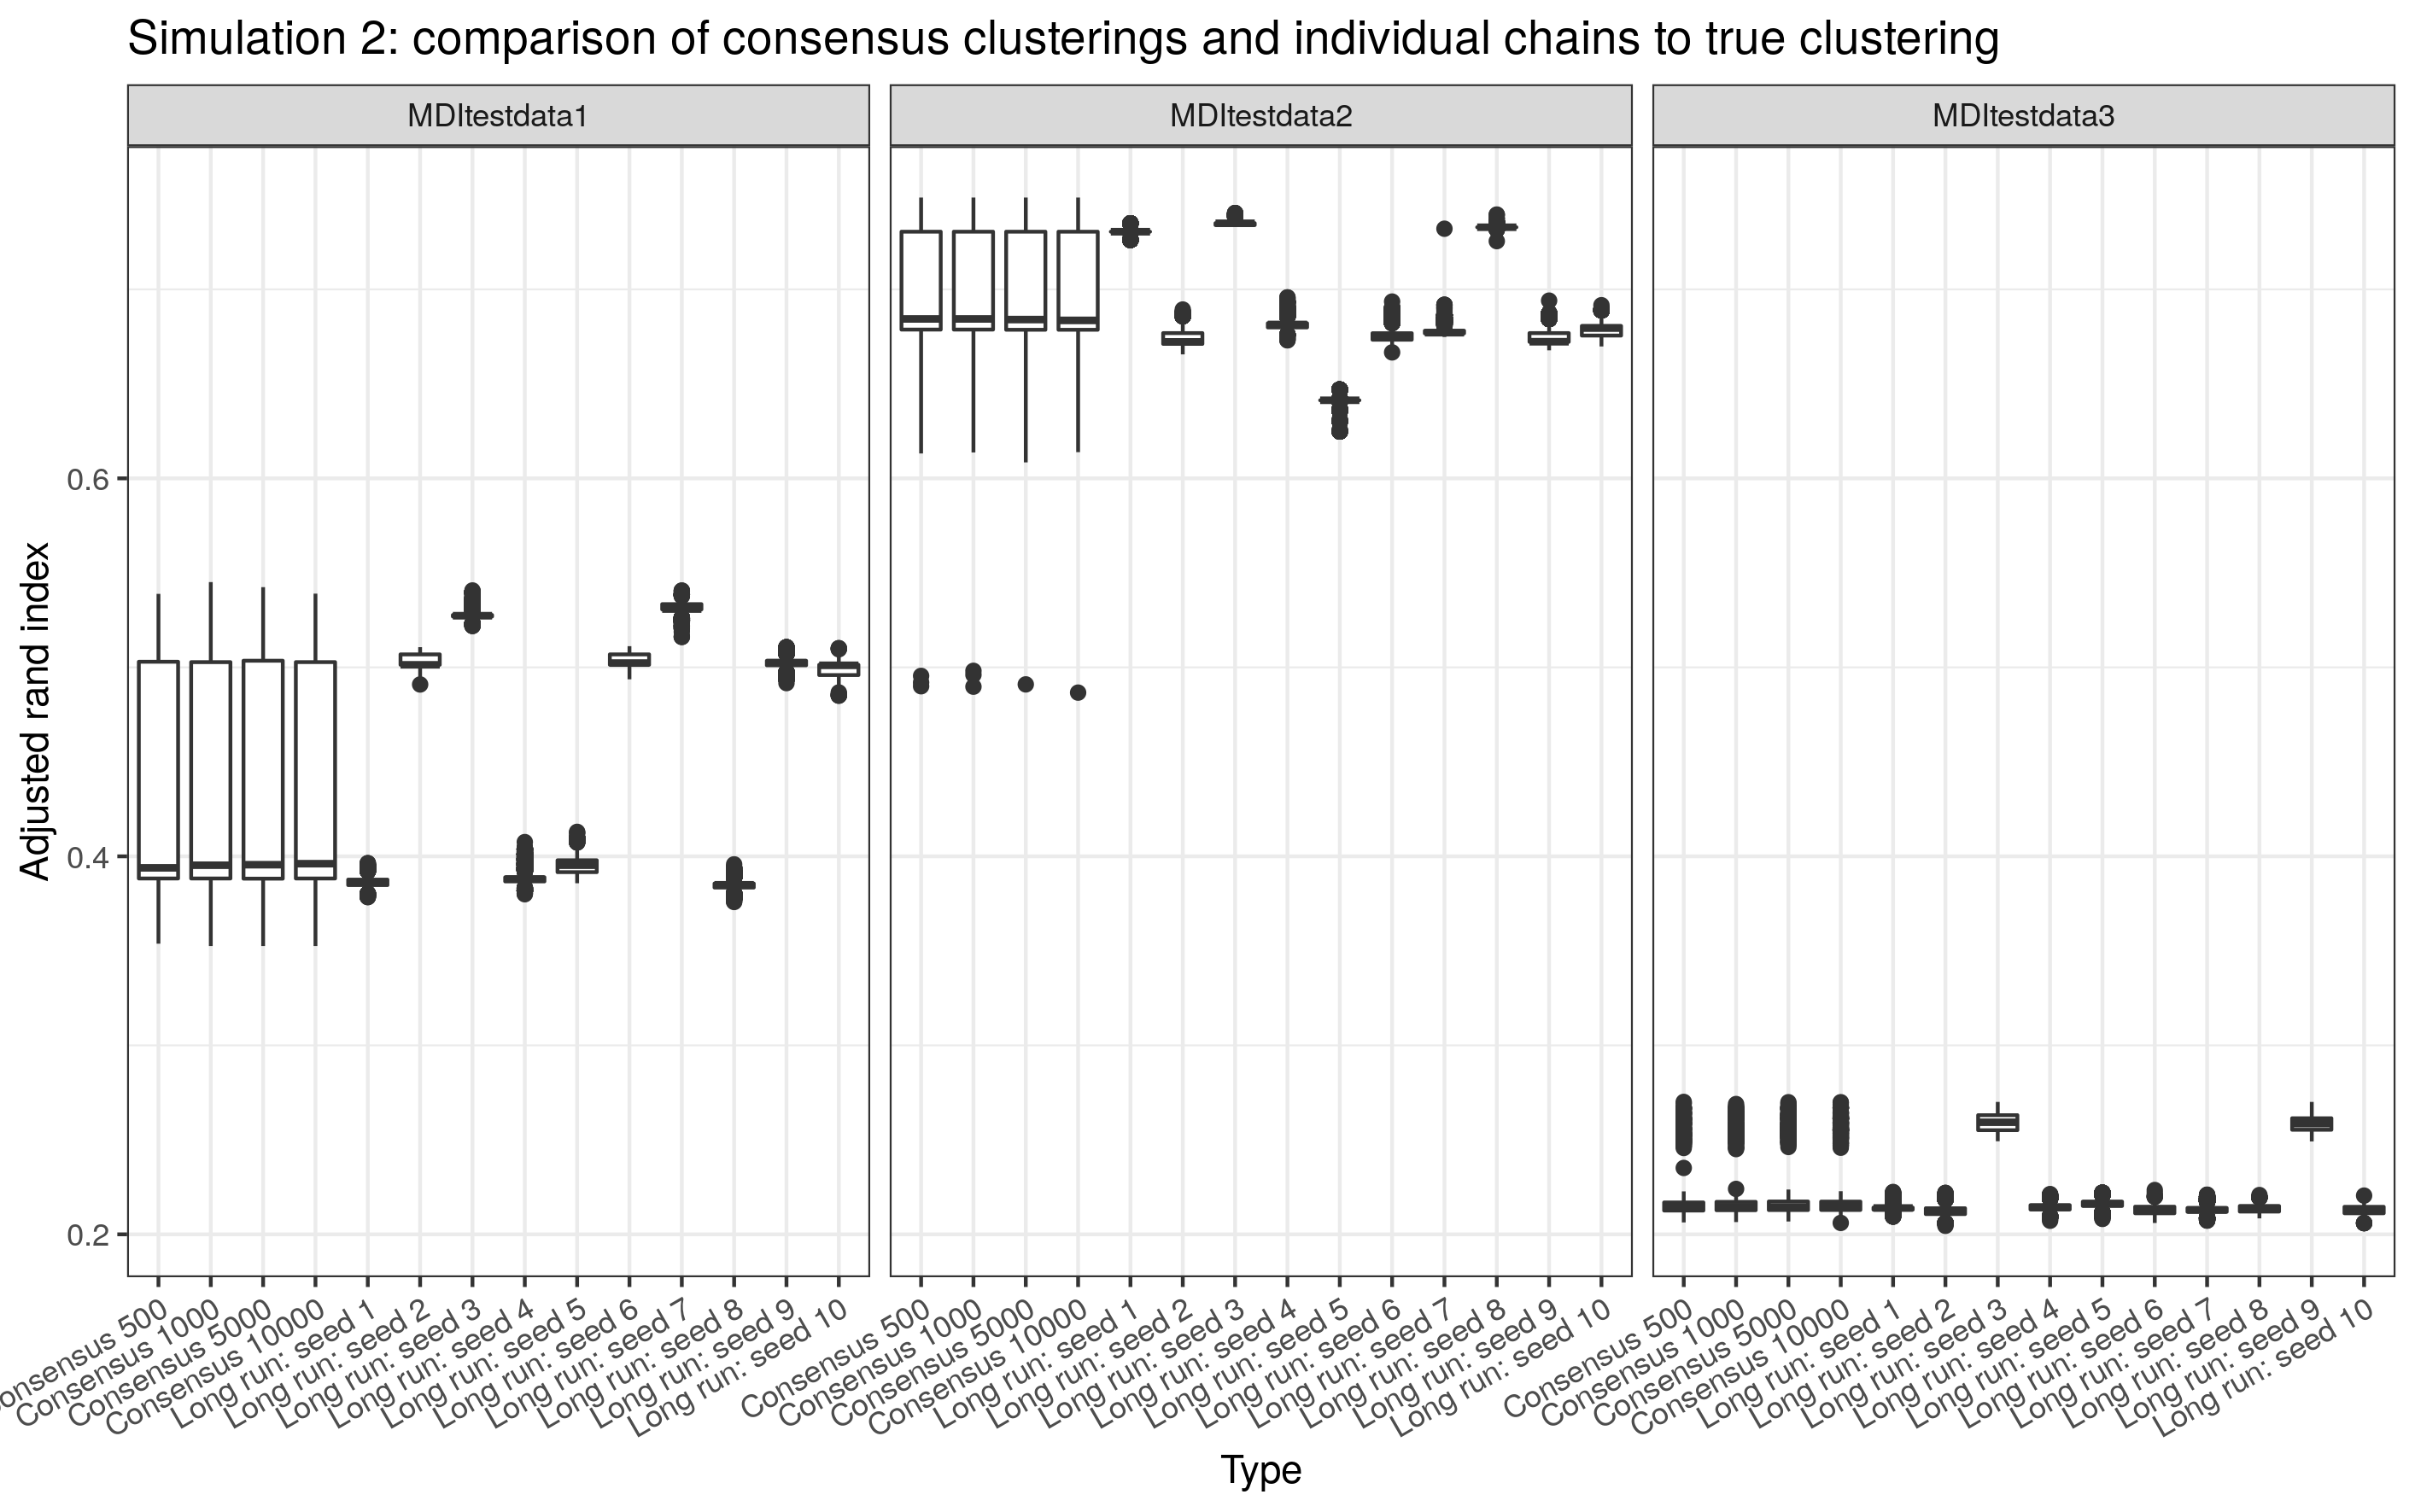
\includegraphics[scale=0.9]{Images/Gen_data/Case_2/box_plot_ari_true_clustering_burn_in.png}
		\caption{Box plots for distribution of adjusted rand index between the clustering at each iteration to the true clustering for different lengths of consensus clustering and different initialisation of long chains.}
		\label{fig:gen_data_case_2_boxplot}
	\end{sidewaysfigure}
%	\end{figure}

%	\newpage

	\begin{figure}[!htb]
		\centering
		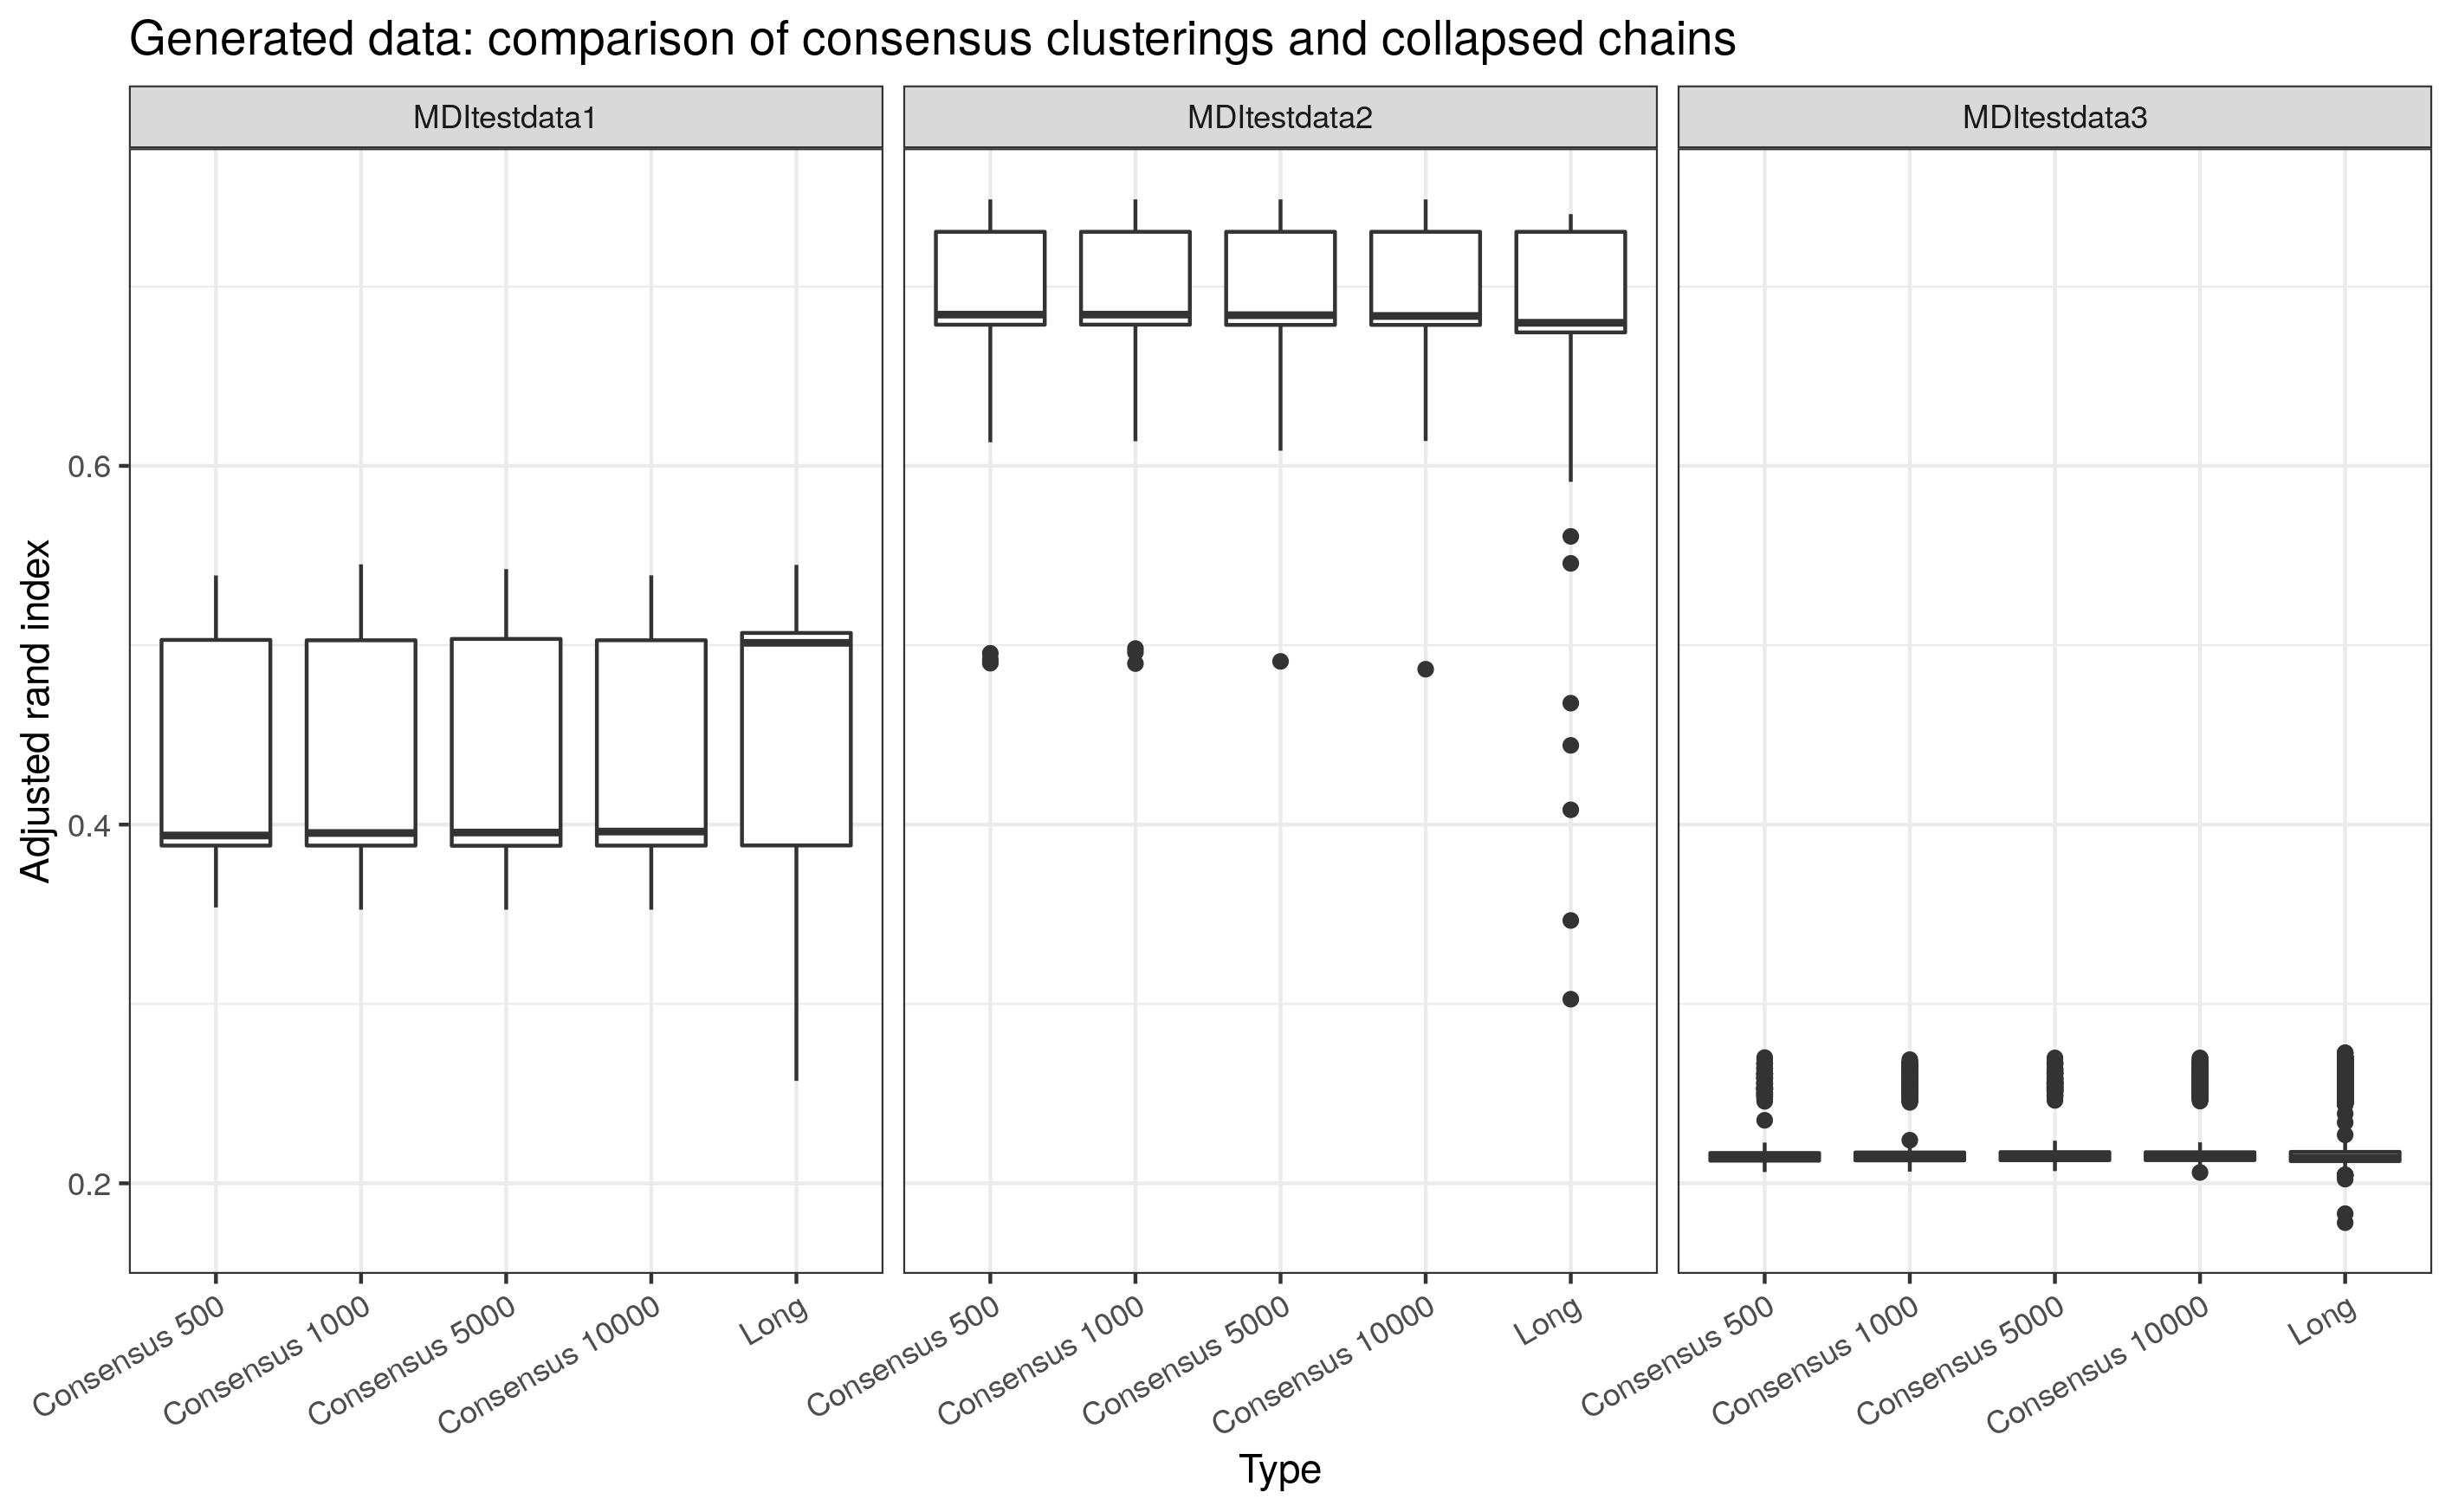
\includegraphics[scale=0.65]{Images/Gen_data/Case_2/box_plot_ari_true_clustering_collapsed_long.png}
		\caption{Box plots for distribution of adjusted rand index between the clustering at each iteration to the true clustering for different lengths of consensus clustering and the collapsed long chains.}
		\label{fig:gen_data_case_2_collapsed_boxplot}
	\end{figure}
	
%	\newpage

	\begin{figure}[h]
		\centering
		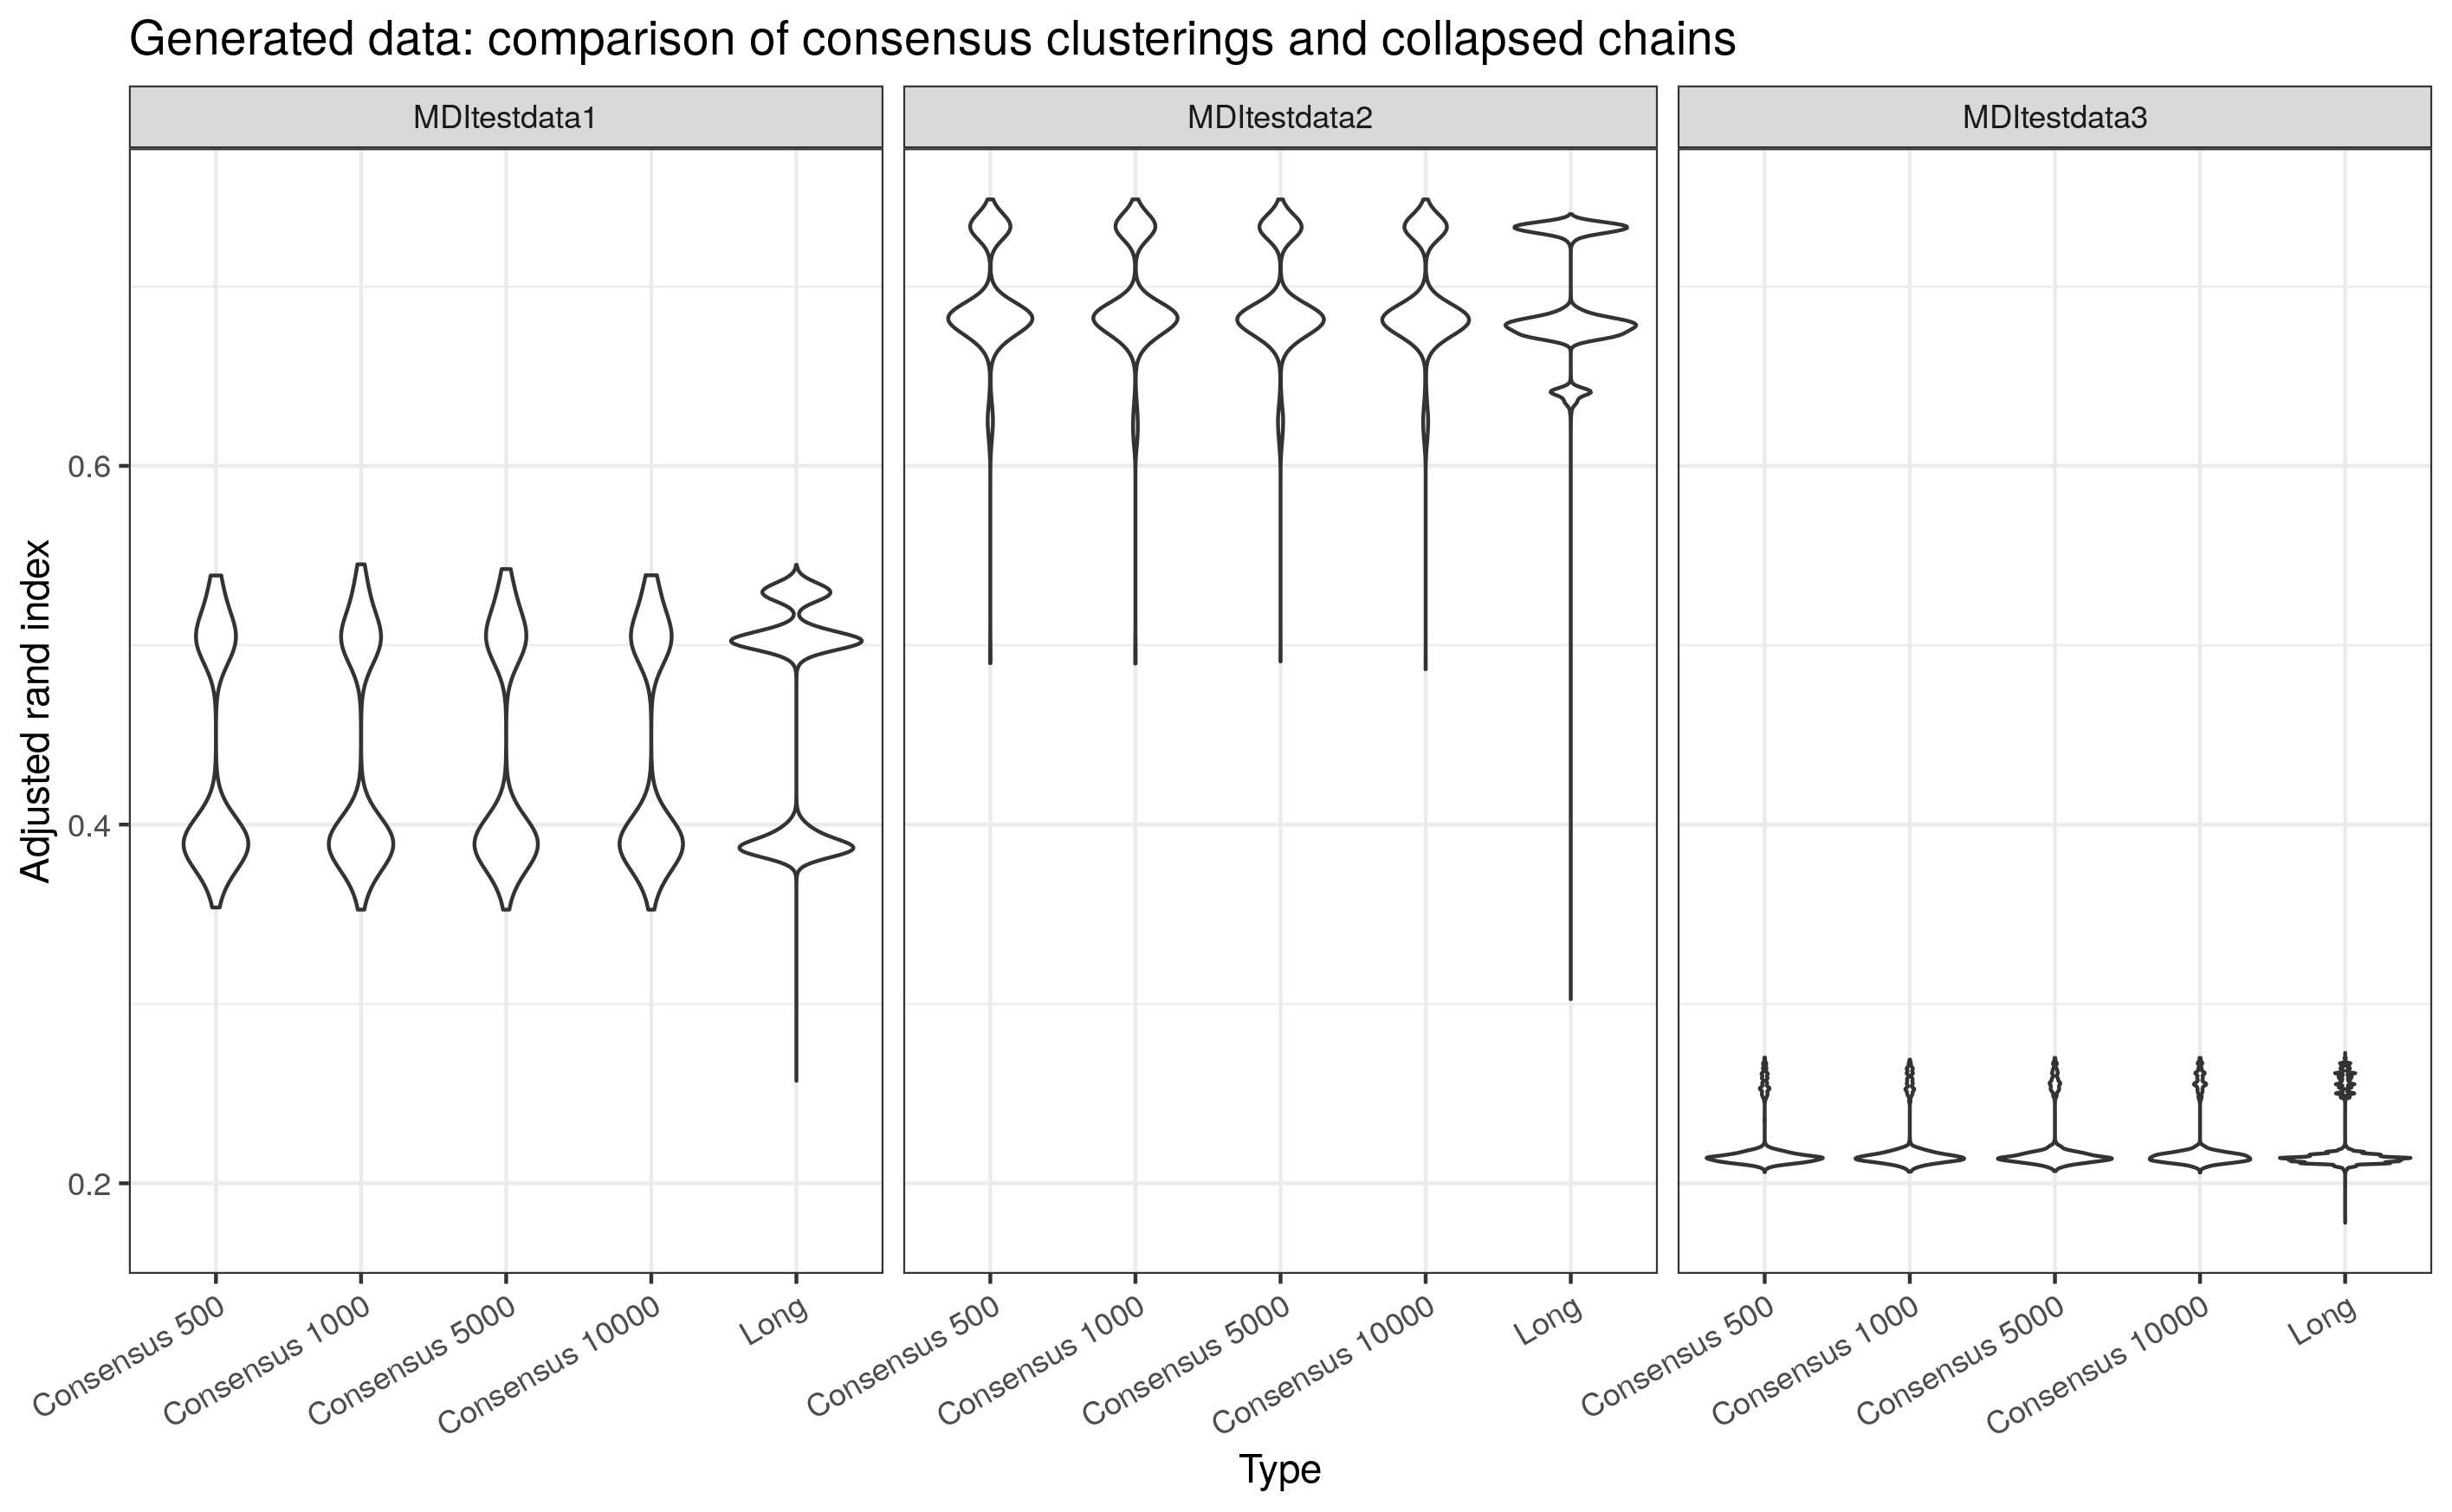
\includegraphics[scale=0.65]{Images/Gen_data/Case_2/violin_plot_ari_true_clustering_collapsed_long.png}
		\caption{Violin plots for distribution of adjusted rand index between the clustering at each iteration to the true clustering for different lengths of consensus clustering and the collapsed long chains. We can see that the consensus clustering approximates the modes described across chains quite well.}
		\label{fig:gen_data_case_2_collapsed_violin_plot}
	\end{figure}

%	\newpage

	\subsection{CEDAR dataset} \label{sec:results:cedar}
	\subsubsection{Case 1: 250 probes} \label{sec:results:cedar:dataset_1}
%	Consensus clustering with MDI $n_{iter}=500$ and $n_{seeds}=1000$ was implemented on 7 datasets. The datasets were defined as described in section \ref{sec:case_studies:cedar:dataset_1}. Individual mixture models were also run on each dataset for the same number of seeds and iterations as a comparison. 
	
	Each MDI chain of 500 iterations took approximately 7 hours and 20 minutes to run (thus long individual chains were beyond the limits imposed by the available computing power). The output was inspected under multiple lenses: 
	
	\begin{enumerate}
		\item The adjusted Rand index plot in figure \ref{fig:results:cedar_1:mdi_cd4_adj_rand_ind_plot} and the number of clusters present in each seed shown in figure \ref{fig:results:cedar_1:mdi_cd4_mass_parameter_plot} shows that the seeds are exploring different spaces. Figure \ref{fig:results:cedar_1:mdi_cd4_adj_rand_ind_plot} specifically shows the clusterings across each seed are quite similar.
		\item From the mean adjusted Rand index comparing clusterings across datasets in figure \ref{fig:results:cedar_1:mdi_adj_rand_ind_heatmap} one can see that the CD datasets have similar clustering structure as do the intestinal samples, with IL being slightly more distinct from RE and TR. This result is reinforced by figure \ref{fig:results:cedar_1:mdi_phi_heatmap}; here there is further granularity and one can see that within the sets previously mentioned, there are subsets of $\{$CD4, CD8$\}$ and $\{$RE, TR$\}$.
		\item The $\phi_{ij}$ values in figures \ref{fig:results:cedar_1:mdi_re_tr_phi_series_plot} and \ref{fig:results:cedar_1:mdi_re_tr_phi_histogram} show that the $\phi$ parameter is behaving as expected. It is varying across seeds with different seeds aligning different datasets more strongly (as can be seen in the tails of figure \ref{fig:results:cedar_1:mdi_re_tr_phi_histogram}).
%		\item The mass parameter for the underlying mixture models, an example of which can be seen in figure \ref{fig:results:cedar_1:mdi_cd4_mass_parameter_plot}, is in keeping with the belief that the MDI model is behaving properly as each mass paramet;
		\item The PSM in figure \ref{fig:results:cedar_1:mdi_cd4_psm} contains several distinct clusters. One can see uncertainty in some of the clusters.
		\item From the comparison of the PSM, the standardised expression data and the correlation matrix in figure \ref{fig:results:cedar_1:mdi_cd4_psm_expr_cor}, one can see that the structure in the correlation matrix is uncovered by the PSM and there are blocks within the standardised expression data which correspond to uncovered clusters in the PSM. %; and
%		\item The expression of fused genes was plotted for all dataset combinations (see an example in  figure \ref{fig:mdi_cd4_cd8_fused_genes}).
	\end{enumerate}
	Note that some of these (such as the $\phi_{ij}$ plots) only apply to MDI, not the mixture models as this is the single dataset case and comparisons across datasets are not possible.

	\newpage
	
	\begin{figure}[h]
		\centering
		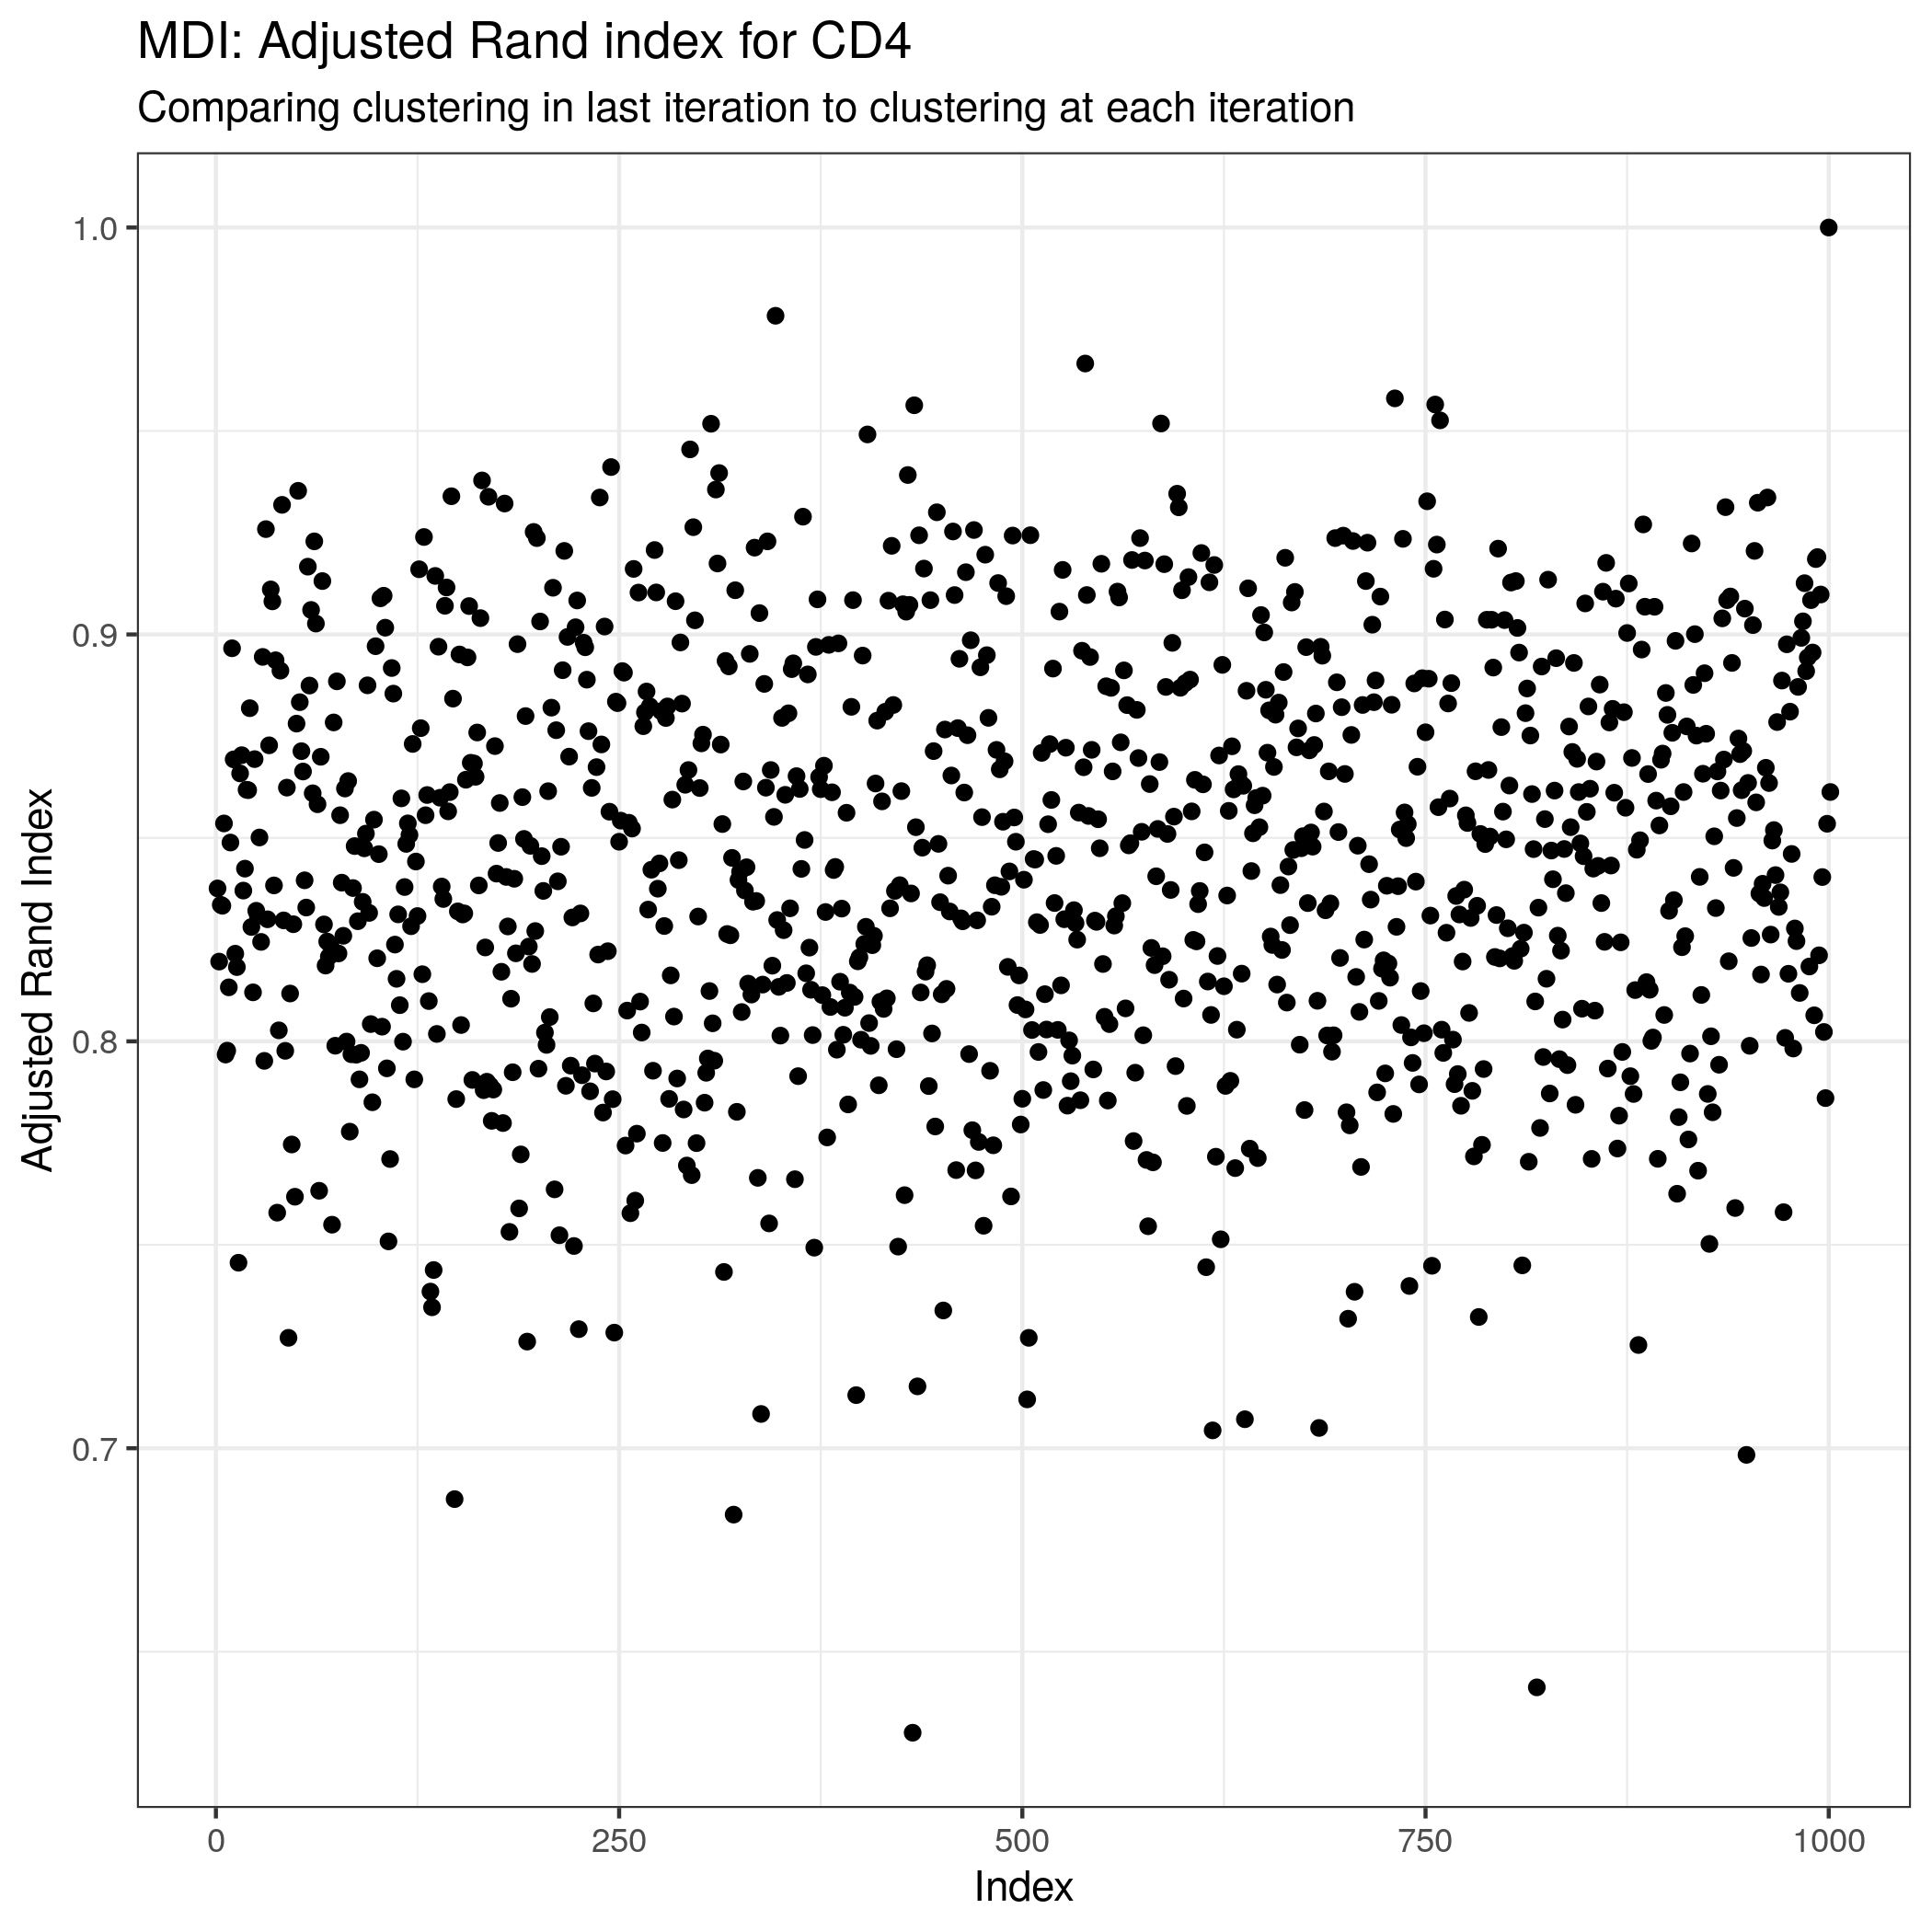
\includegraphics[scale=0.75]{Images/Biology_data/Set_250/All_datasets/Adjusted_rand_index_plots/rand_index_plot_CD4.png}
		\caption{CEDAR Case 1: Plot of the adjusted Rand index between the clustering in each seed to that in the 1,000$^{th}$ for CD4. The narrow range of values present suggests each chain is describing clusters with some similarity, but that there is some variety.}
		\label{fig:results:cedar_1:mdi_cd4_adj_rand_ind_plot}
	\end{figure}
	
	\newpage
	
	\begin{figure}[h]
		\centering
		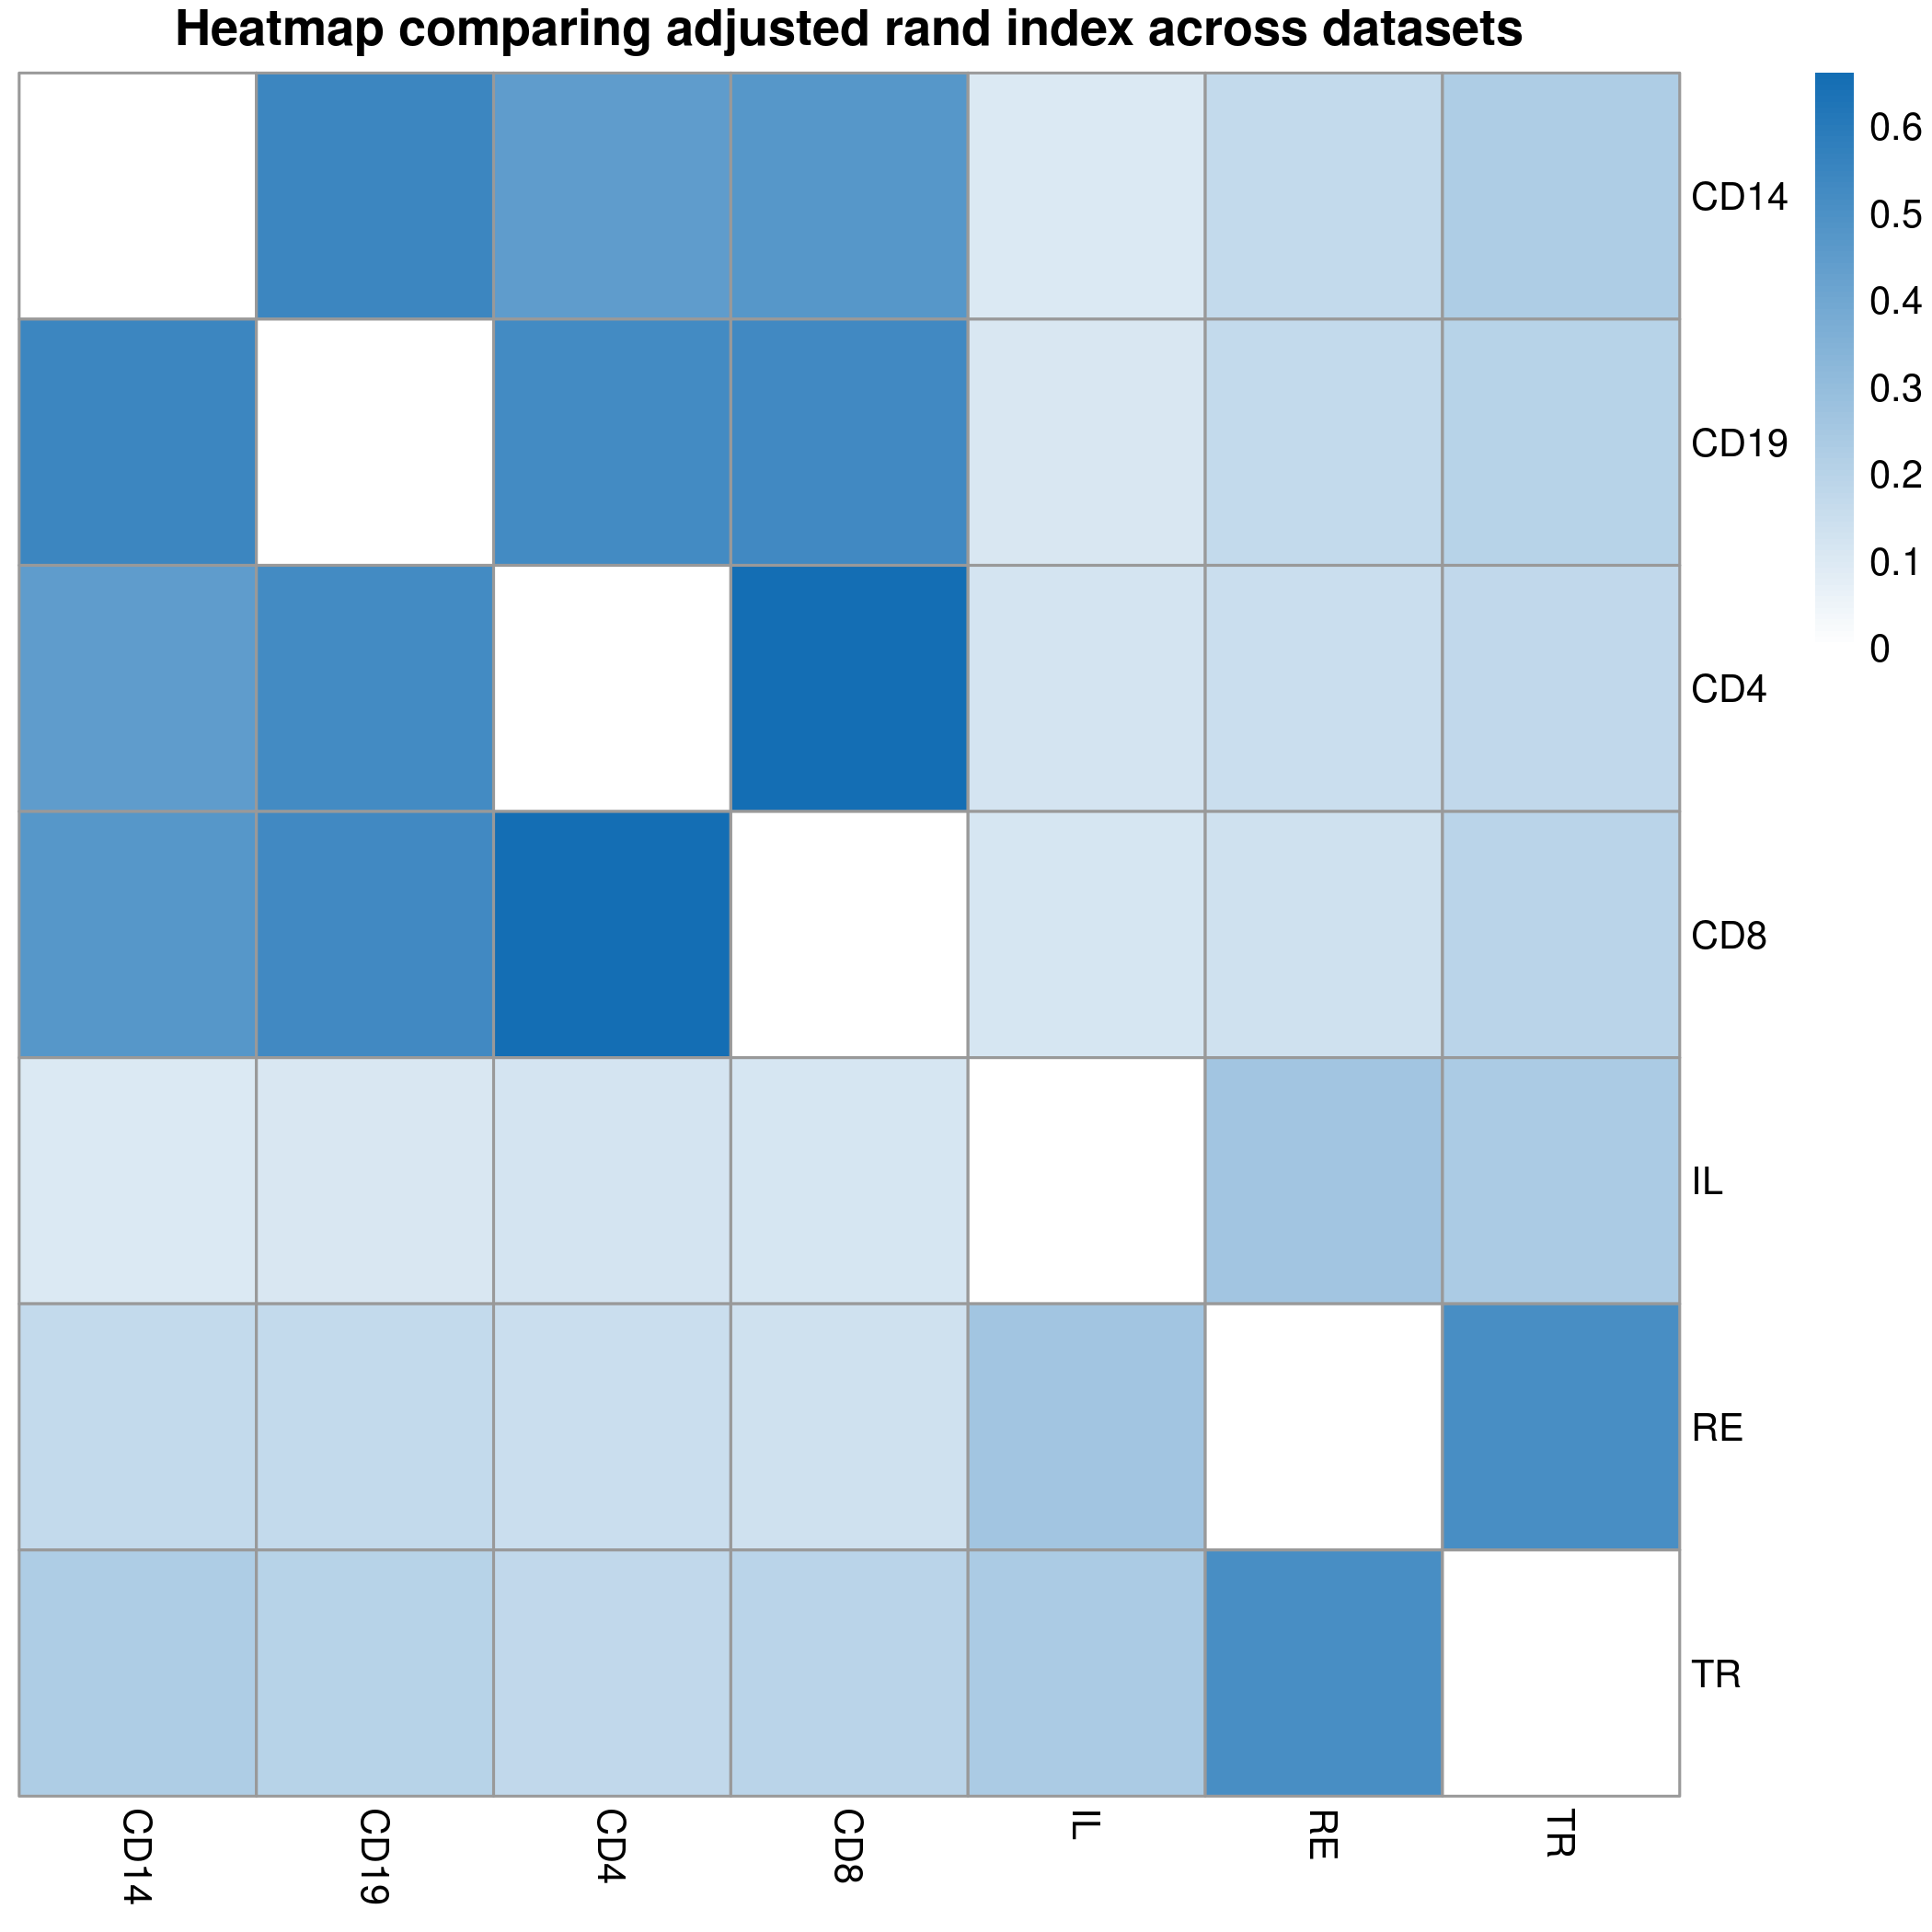
\includegraphics[scale=0.75]{Images/Biology_data/Set_250/All_datasets/Arandi_heatmap.png}
		\caption{CEDAR Case 1: Heatmap of the mean adjusted Rand index comparing the clustering across datasets for each seed. One can see that the CD datasets have similar clustering structure as do the intestinal samples. IL is slightly more distinct from RE and TR, which might be expected as ileum is a distinct organ from the colon.}
		\label{fig:results:cedar_1:mdi_adj_rand_ind_heatmap}
	\end{figure}
	
	\newpage
	
	\begin{figure}[h]
		\centering
		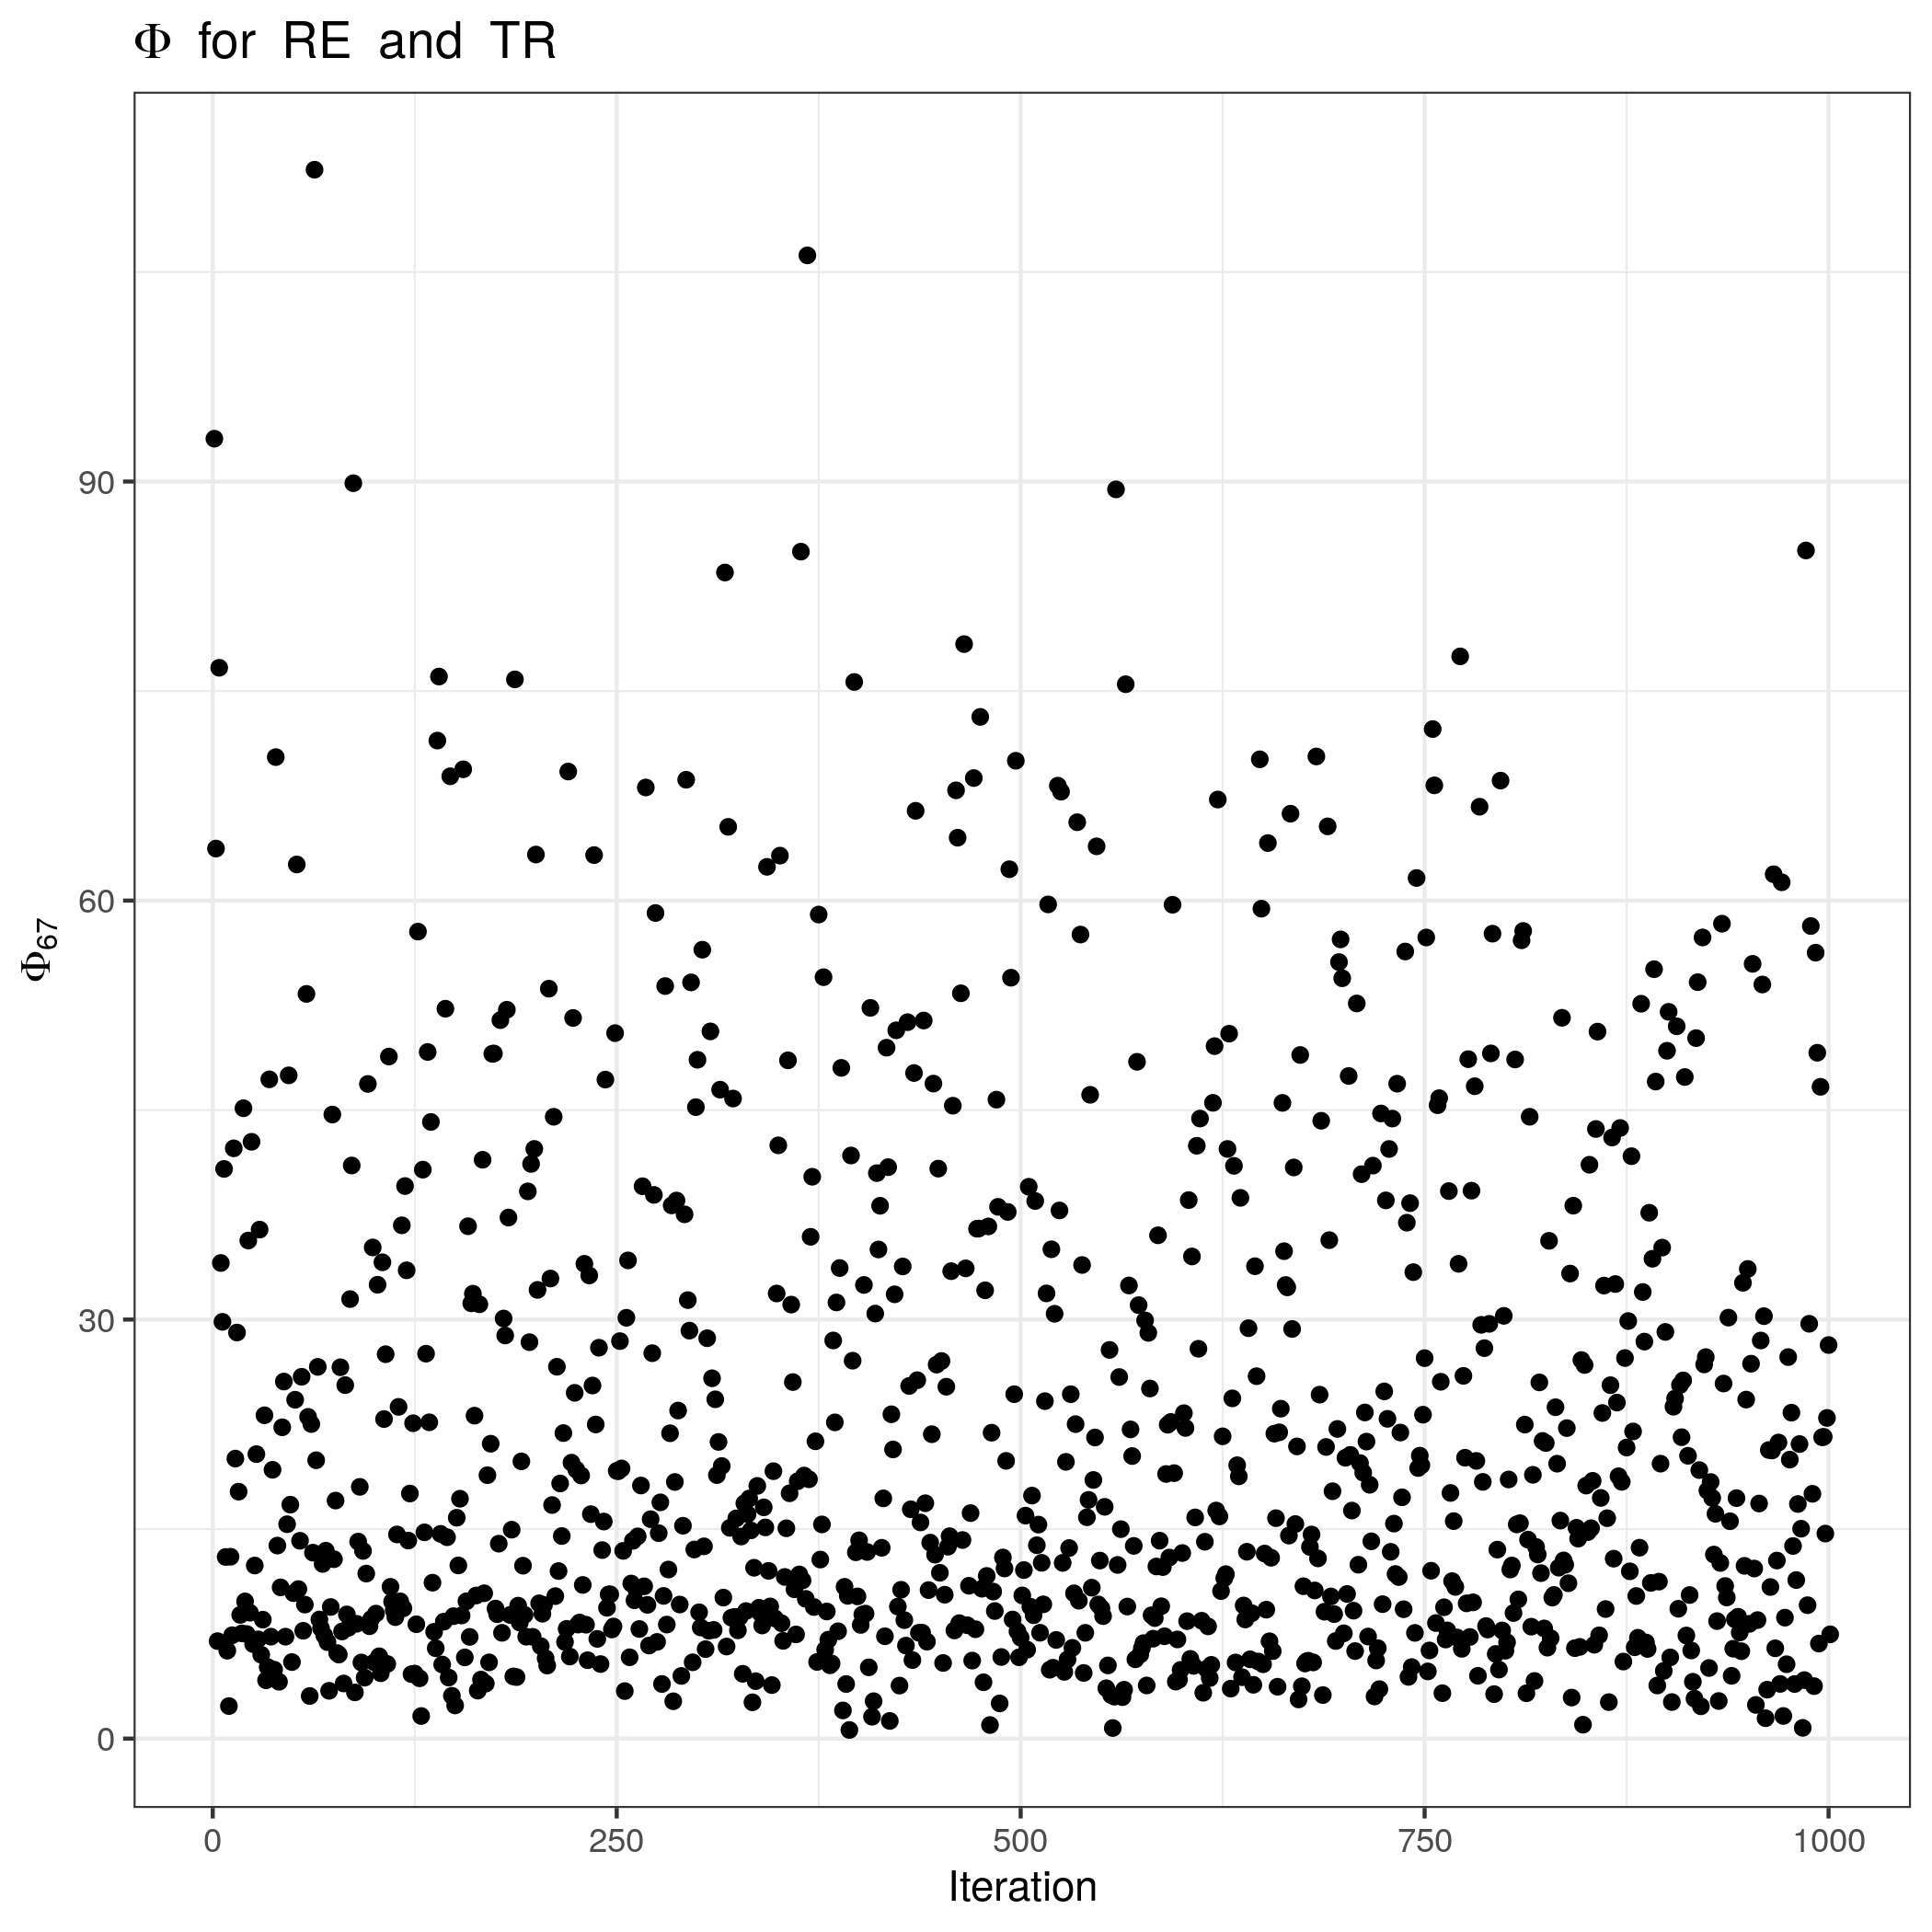
\includegraphics[scale=0.75]{Images/Biology_data/Set_250/All_datasets/Phi_series_plots/file_1_Phi_67.png}
		\caption{CEDAR Case 1: Plot of the $\phi_{67}$ values across all seeds, between the RE and TR datasets (note that the high values indicate a high clustering correlation).}
		\label{fig:results:cedar_1:mdi_re_tr_phi_series_plot}
	\end{figure}

	\newpage
	
	
	
%		\begin{figure}[h]
%		\centering
%		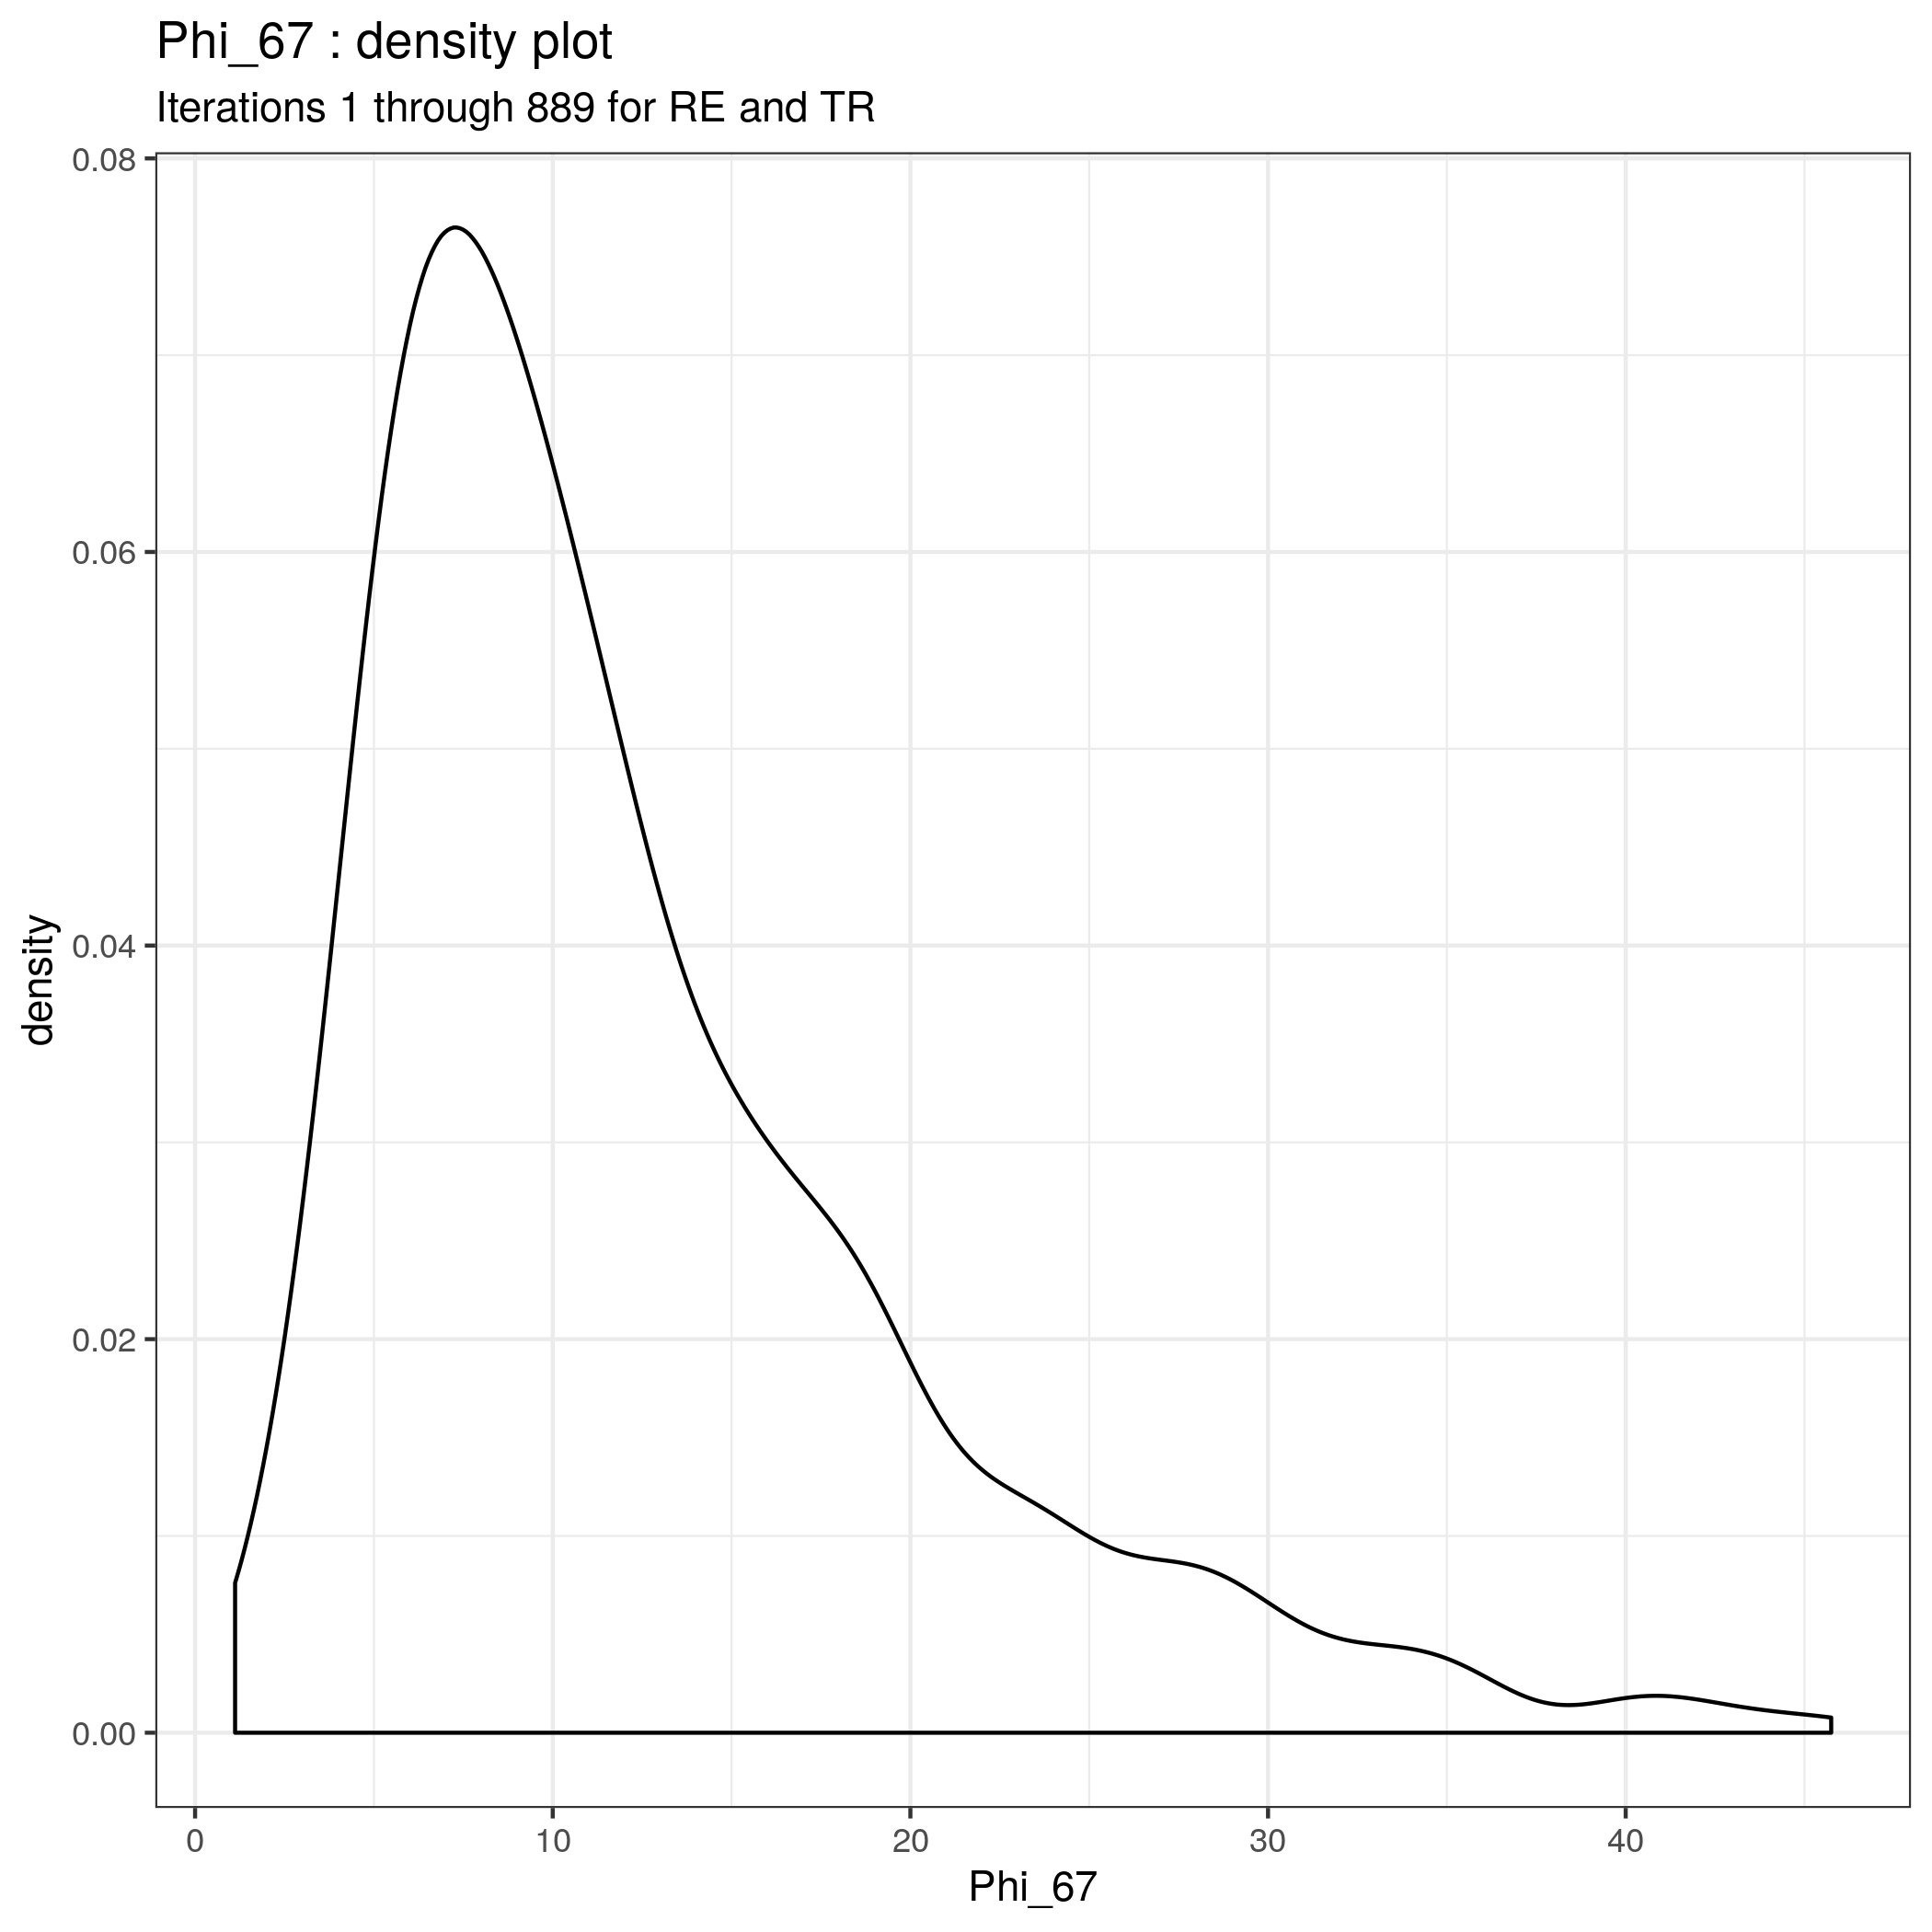
\includegraphics[scale=0.75]{Images/Biology_data/All_datasets/Phi_density_plots/Phi_67_density_plot.png}
%		\caption{Plot of the distribution $\phi_{67}$ values across all seeds, between the RE and TR datasets (note that the high values indicate a high clustering correlation).}
%		\label{fig:mdi_re_tr_phi_density_plot}
%	\end{figure}
%
%	\newpage

	\begin{figure}[h]
		\centering
		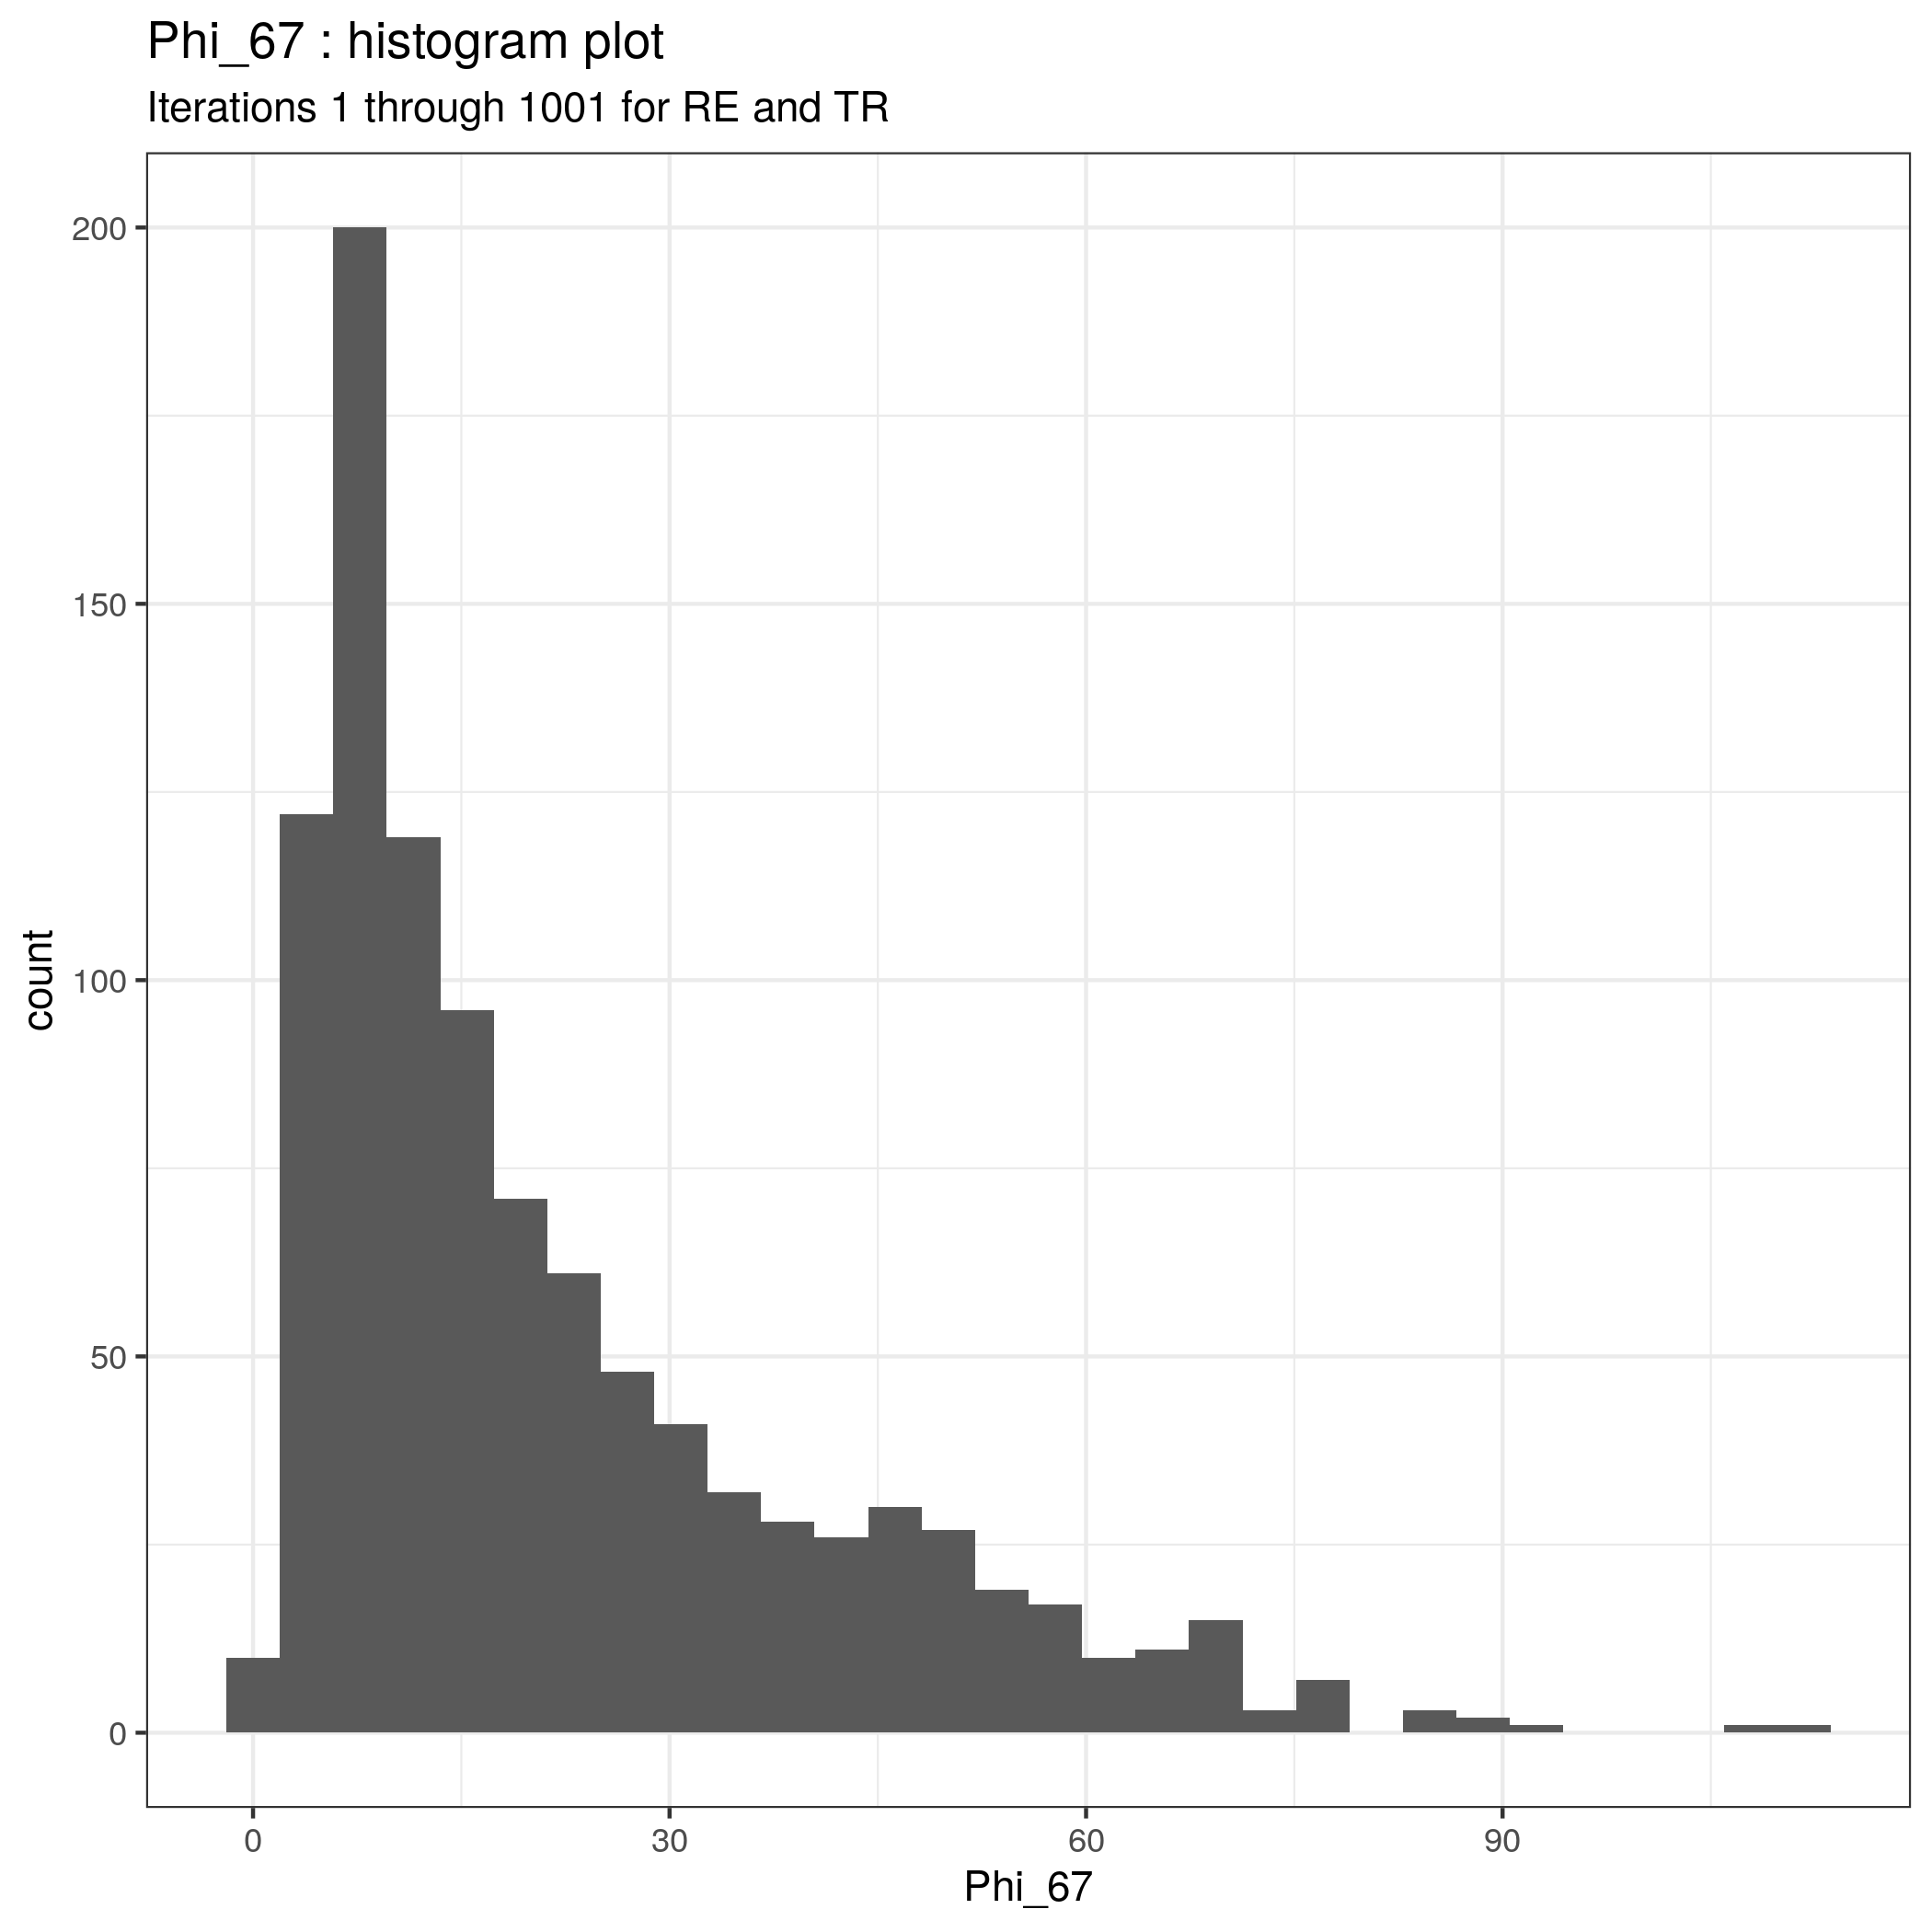
\includegraphics[scale=0.75]{Images/Biology_data/Set_250/All_datasets/Phi_histograms/Phi_67_histogram_plot.png}
		\caption{CEDAR Case 1: Histogram of the distribution of $\phi_{67}$ values across seeds(between the RE and TR datasets).}
		\label{fig:results:cedar_1:mdi_re_tr_phi_histogram}
	\end{figure}
	
	\newpage
	
	
	\begin{figure}[h]
		\centering
		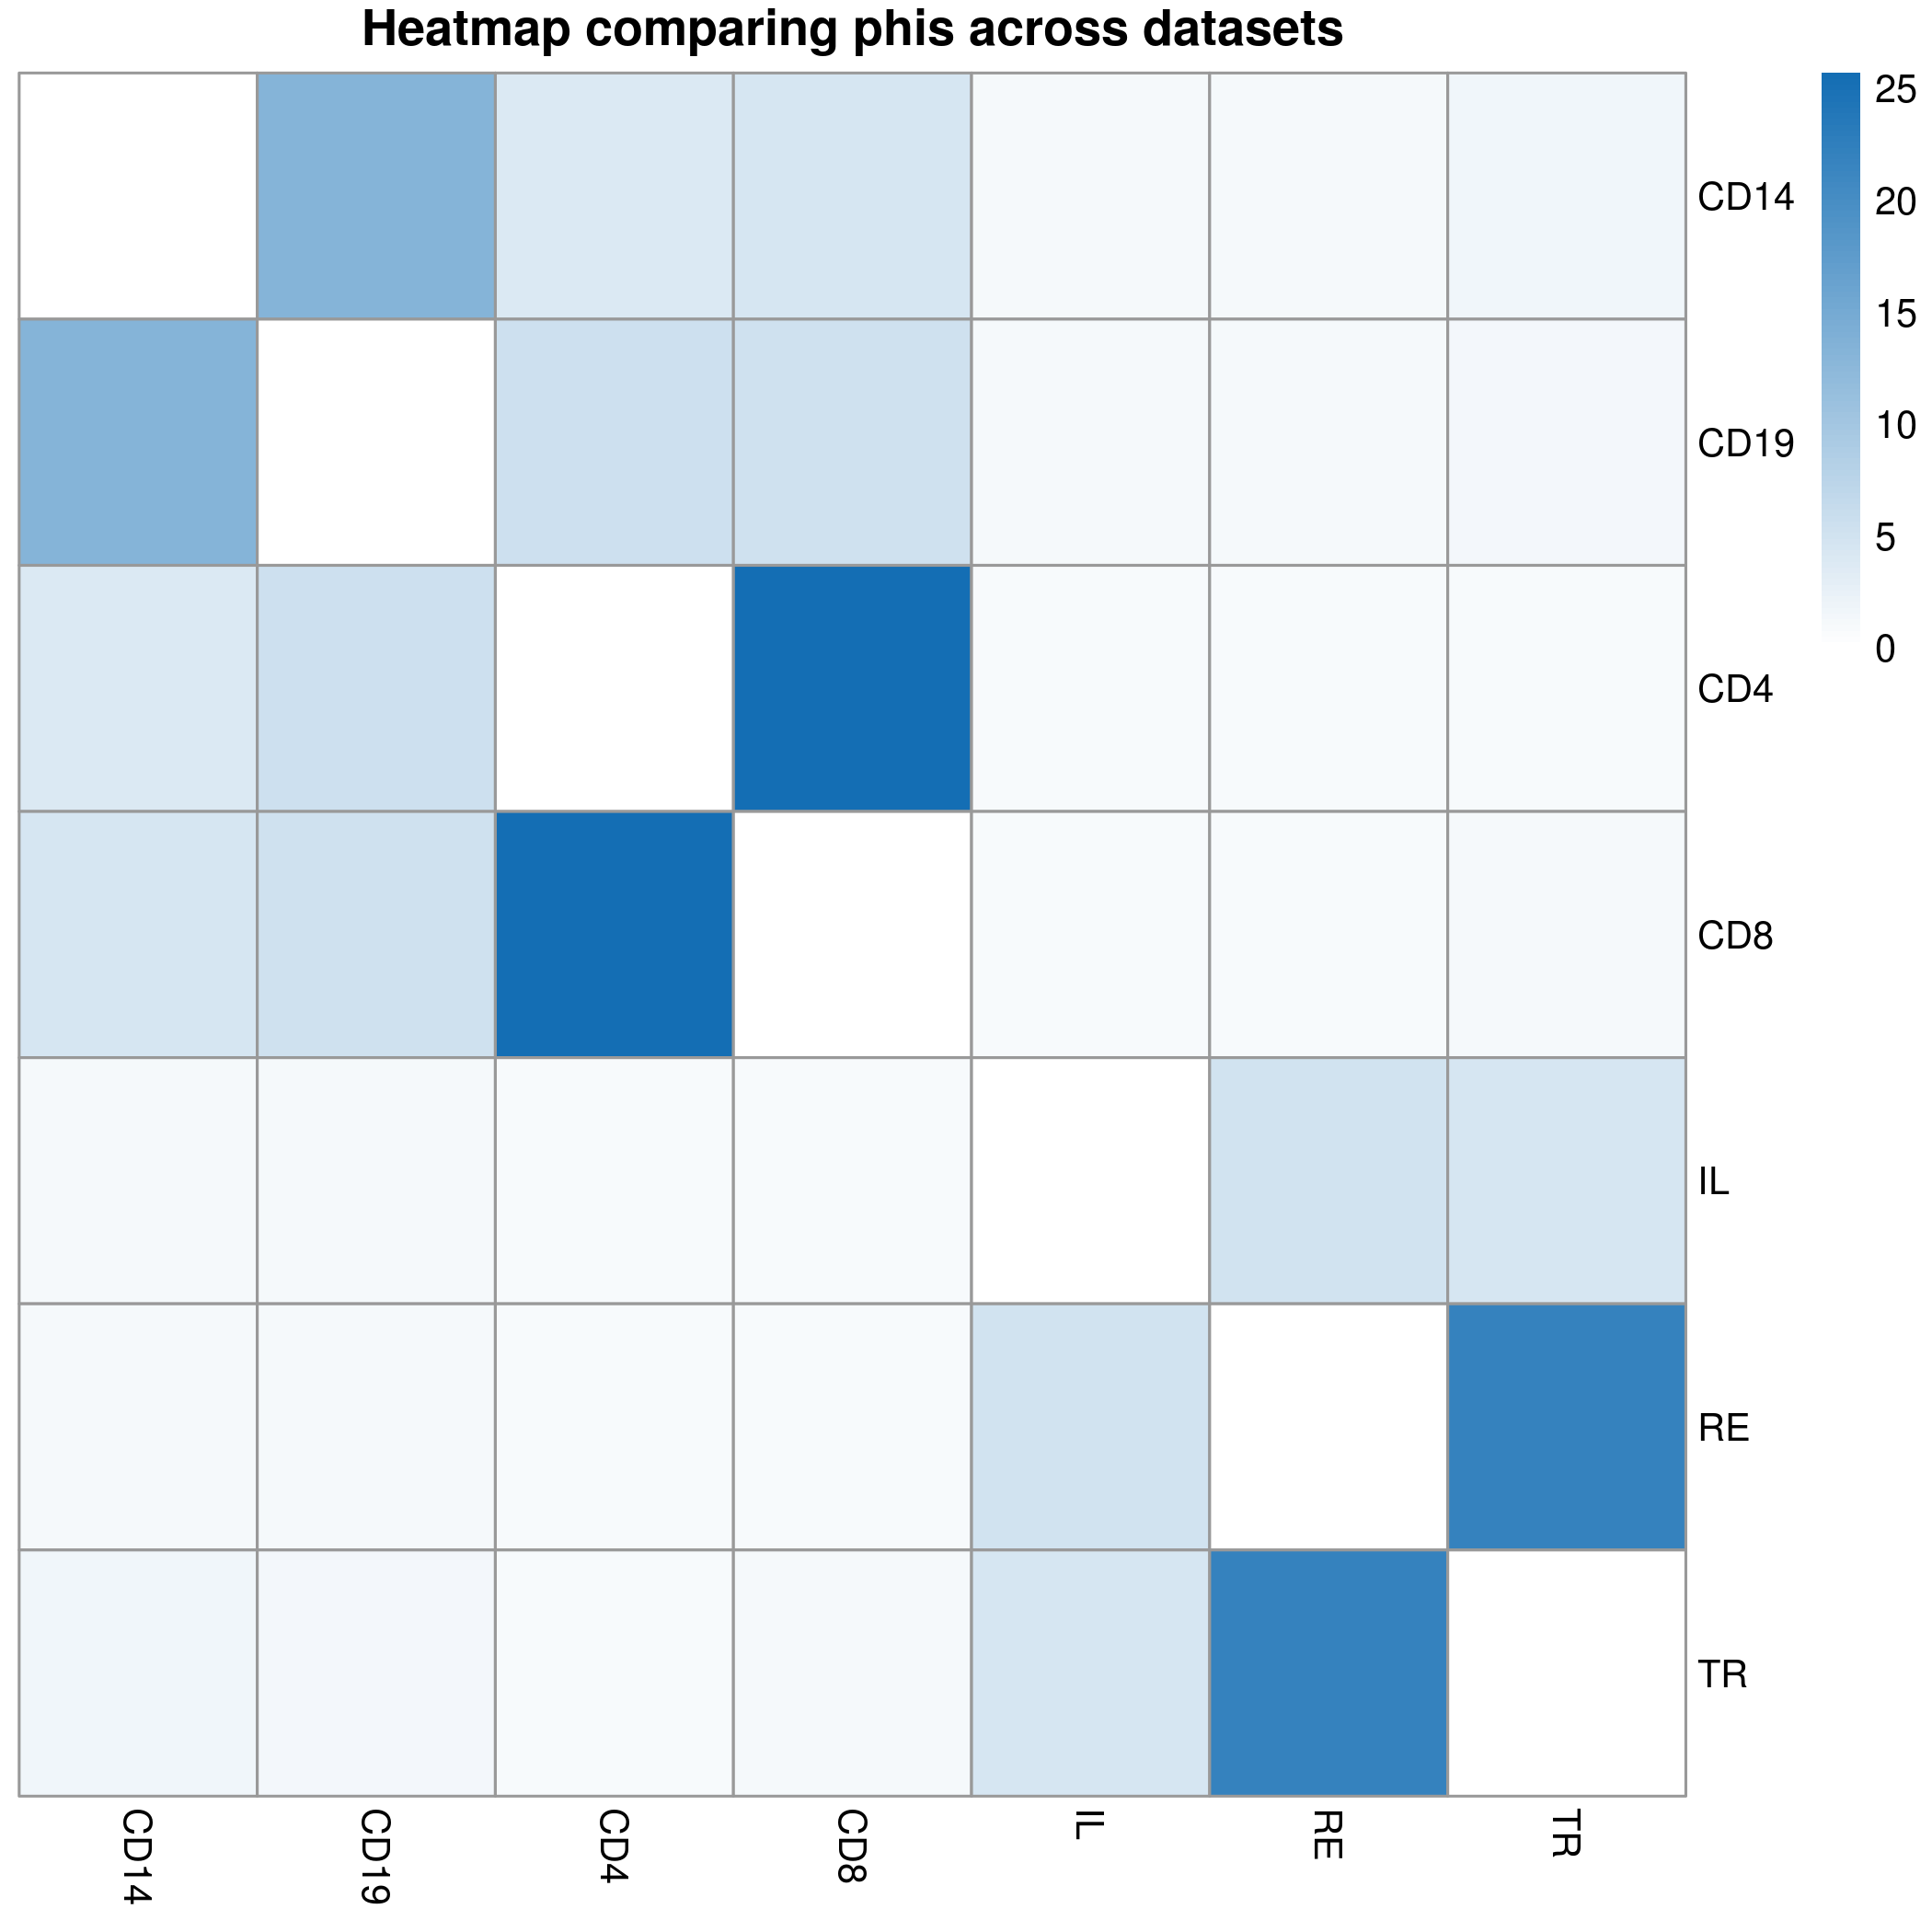
\includegraphics[scale=0.75]{Images/Biology_data/Set_250/All_datasets/Phi_heatmap_1.png}
		\caption{CEDAR Case 1: Plot of the mean $\phi_{ij}$ values across all seeds, between the all datasets. This is very similar to the results depicted in figure \ref{fig:results:cedar_1:mdi_adj_rand_ind_heatmap}, as one would hope. The $\phi_{ij}$ values are meant to quantify similarity between datasets; thus they should mirror the adjusted Rand index between the associated clusterings. Here the specific pairings of $\{$CD4, CD8$\}$ and $\{$RE, TR$\}$ emerge. CD4 and CD8 are both datasets for T cells, while RE and TR are both colonic samples so both these results are satisfactory.}
		\label{fig:results:cedar_1:mdi_phi_heatmap}
	\end{figure}
	
	\newpage


	\begin{figure}[h]
		\centering
		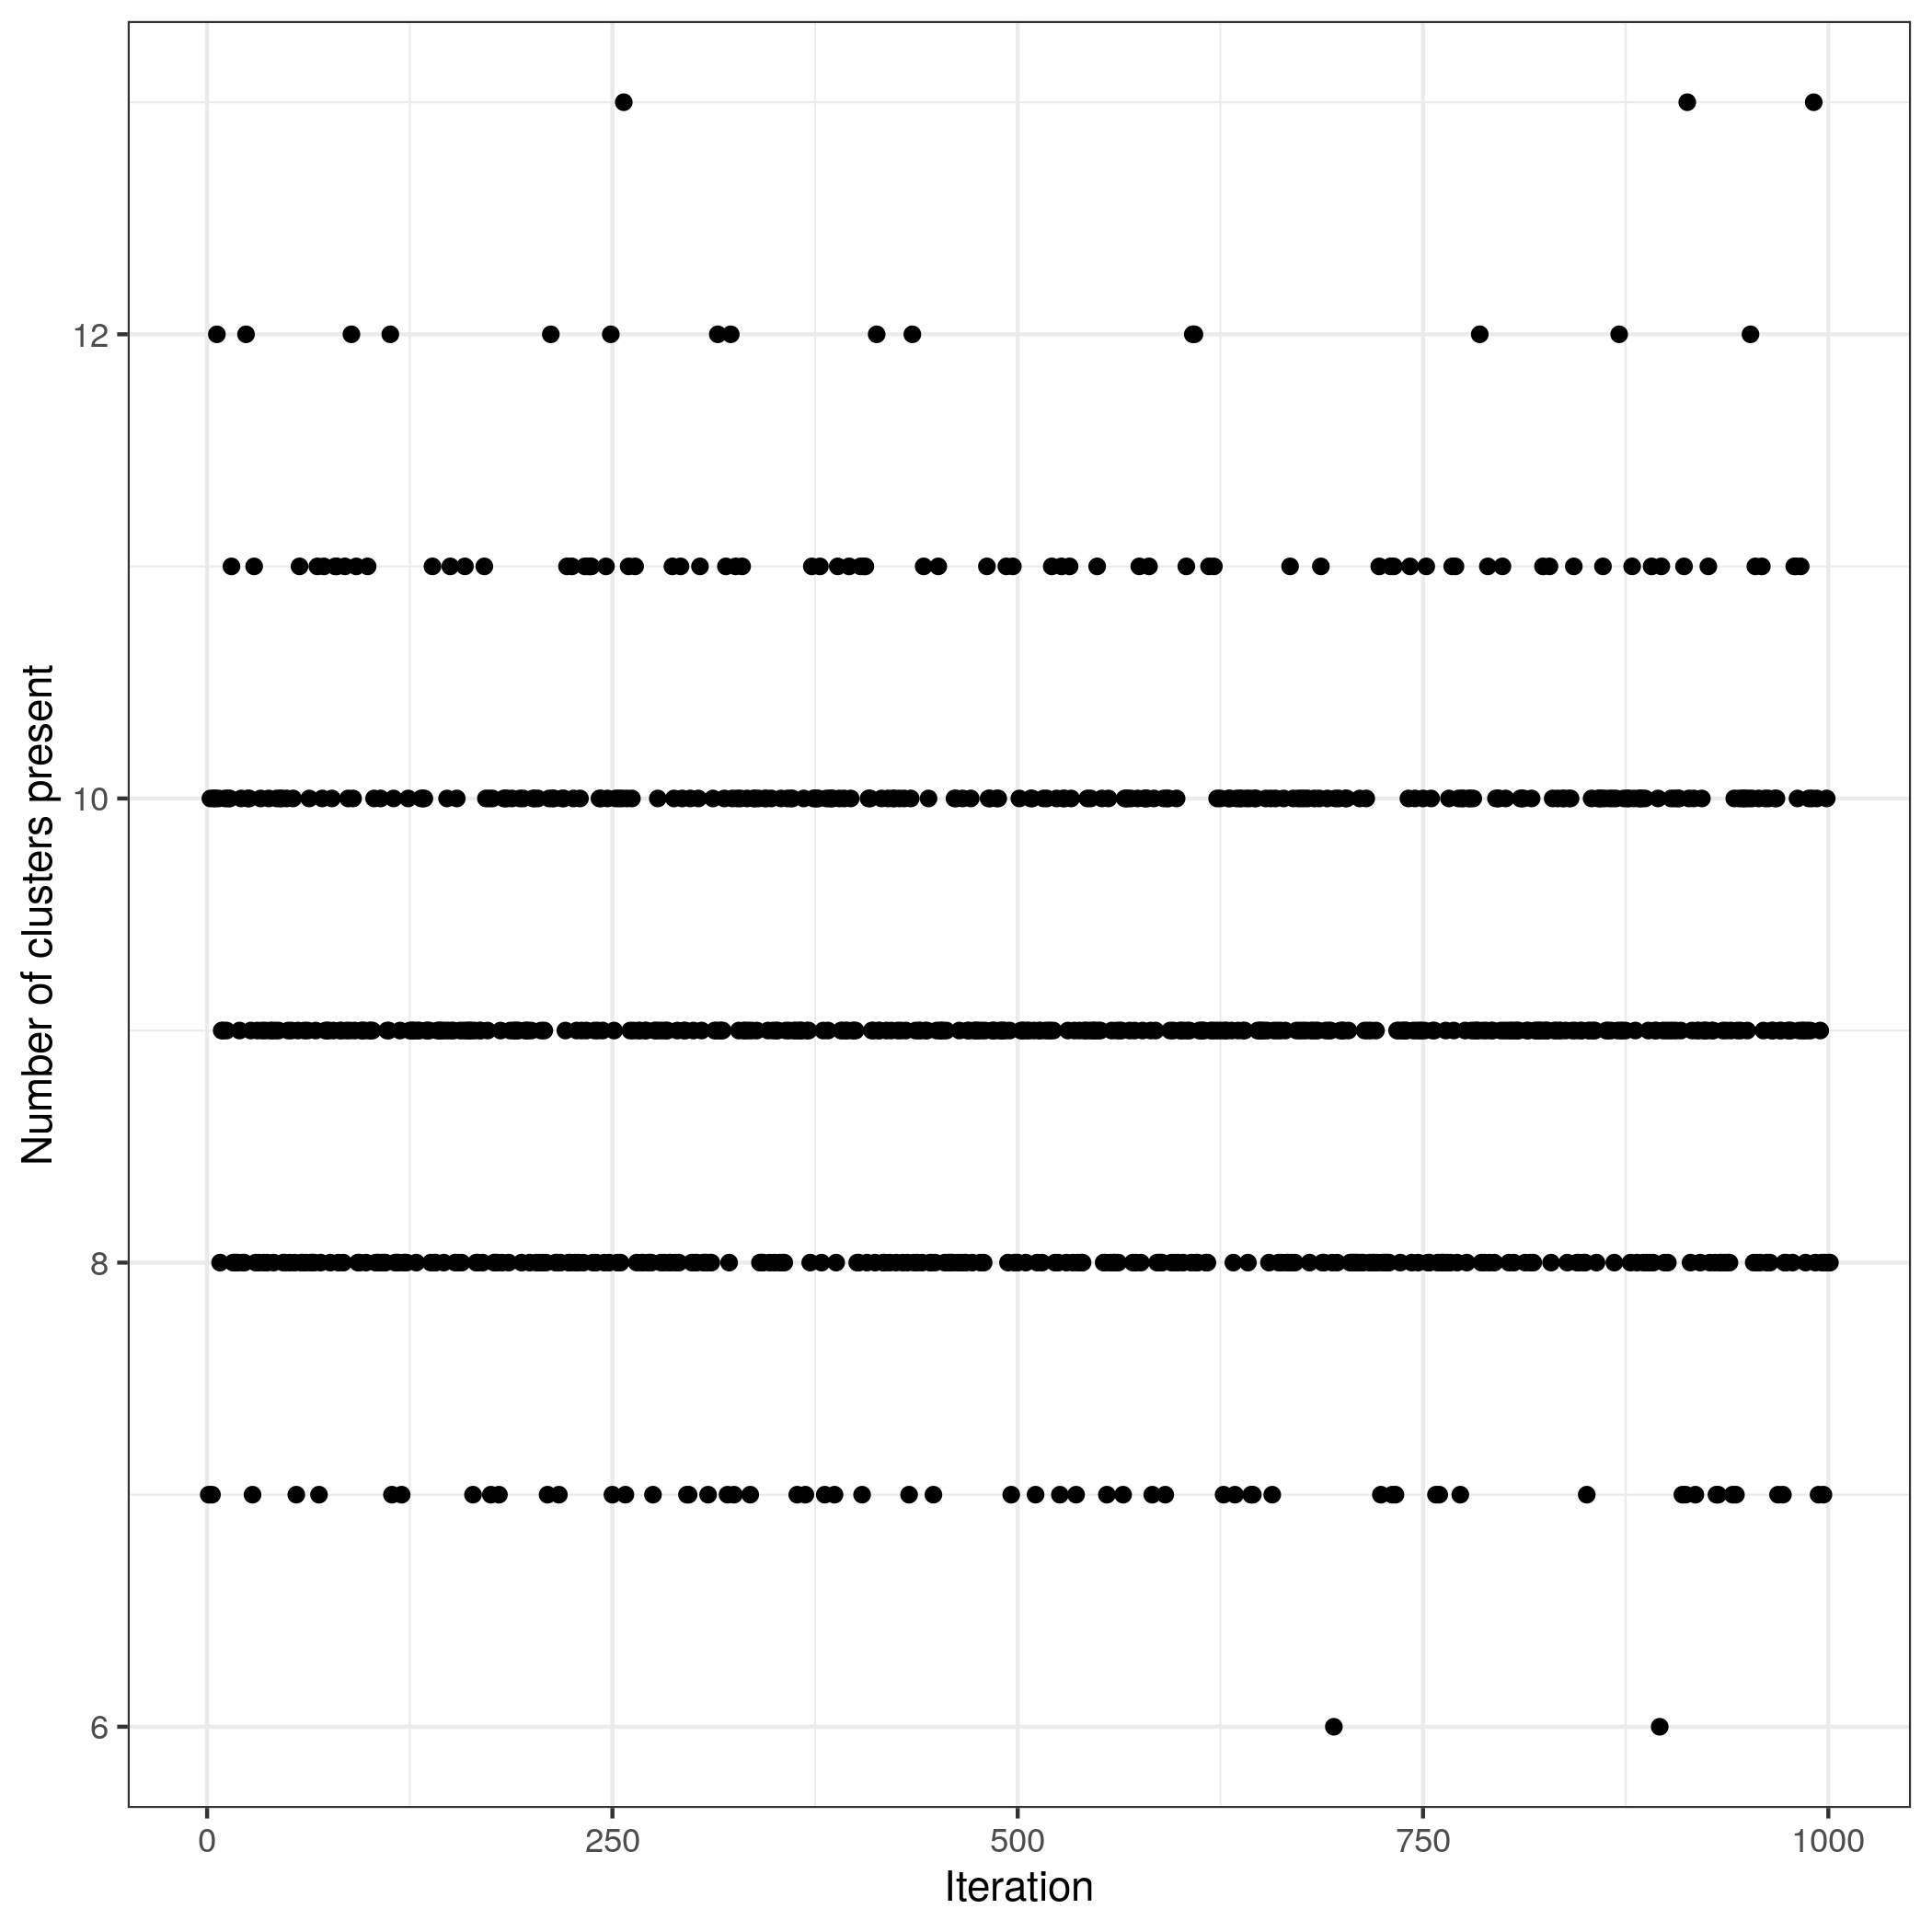
\includegraphics[scale=0.75]{Images/Biology_data/Set_250/All_datasets/Cluster_series_plots/CD4.png}
		\caption{CEDAR Case 1: Plot of the number of clusters present in each seed for the CD4 dataset. It is satisfying to see that different chains explore different configurations.}
		\label{fig:results:cedar_1:mdi_cd4_number_clusters_plot}
	\end{figure}
	
	\newpage
	
	\begin{figure}[h]
		\centering
		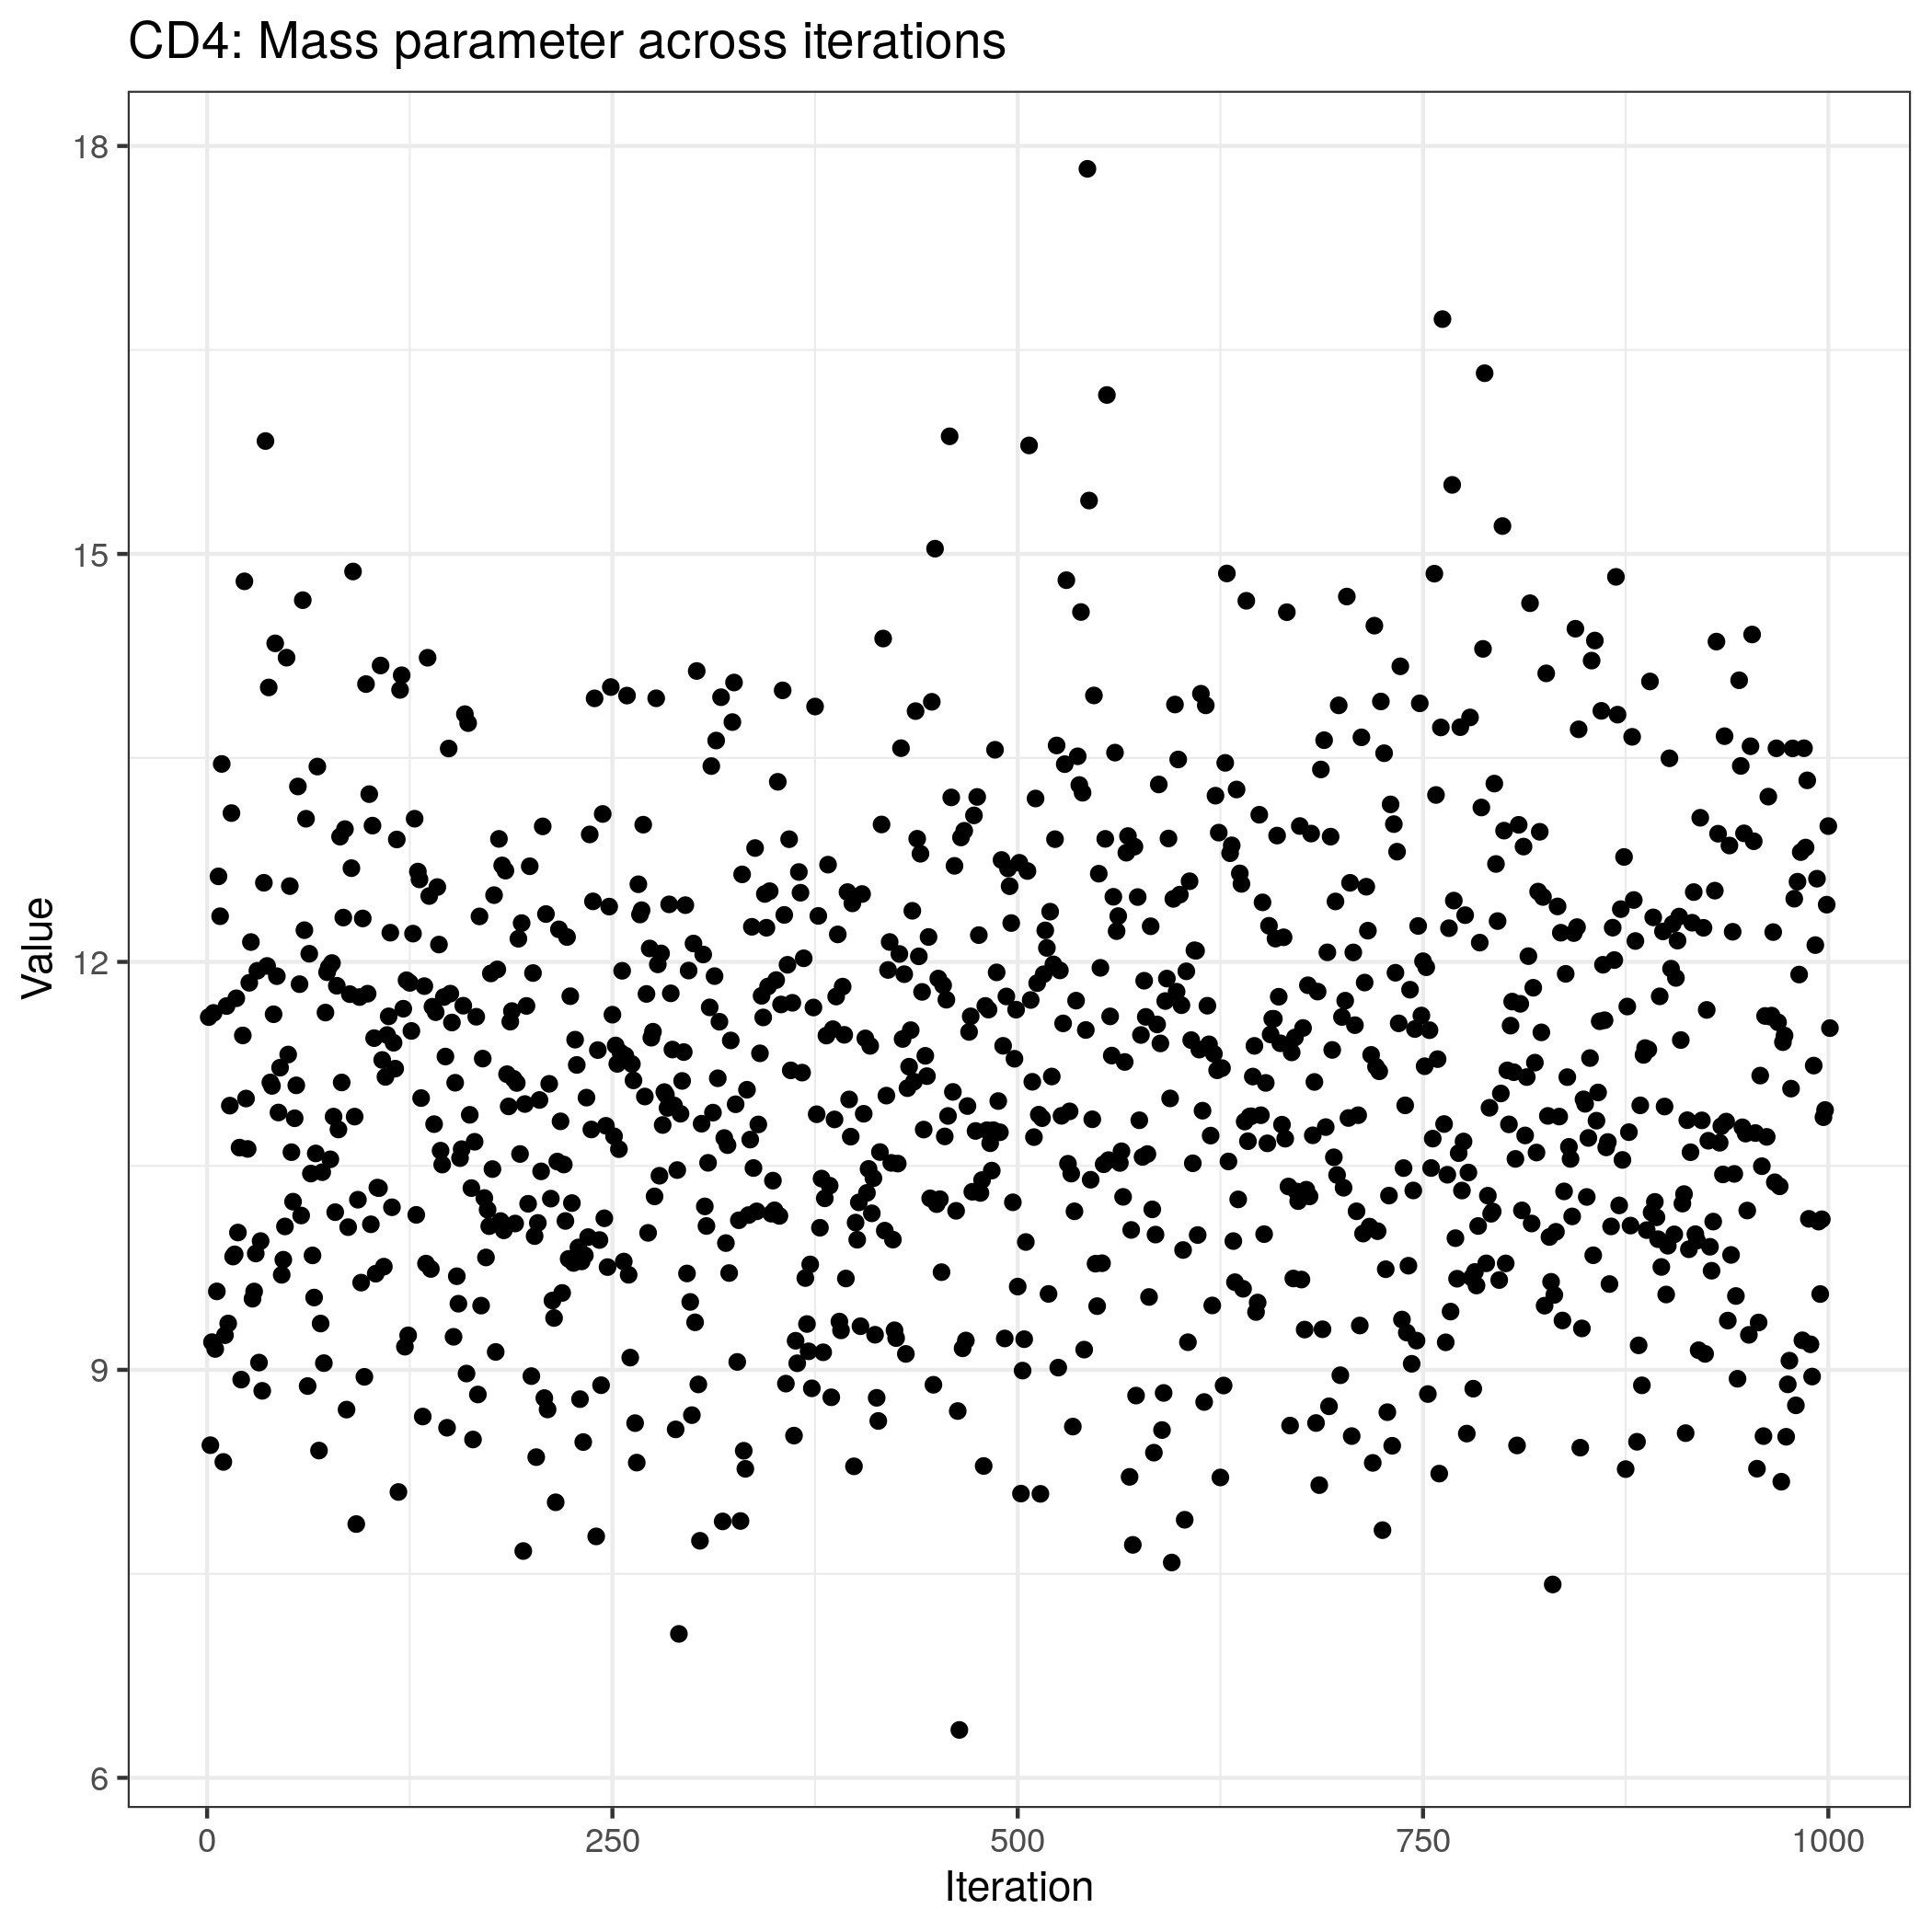
\includegraphics[scale=0.75]{Images/Biology_data/Set_250/All_datasets/Mass_parameter_plots/CD4.png}
		\caption{CEDAR Case 1: Plot of the mass parameter ($\alpha$) for the Dirichlet process for the CD4 dataset of MDI.}
		\label{fig:results:cedar_1:mdi_cd4_mass_parameter_plot}
	\end{figure}
	
	\newpage
	

	
	\begin{figure}[h]
		\centering
		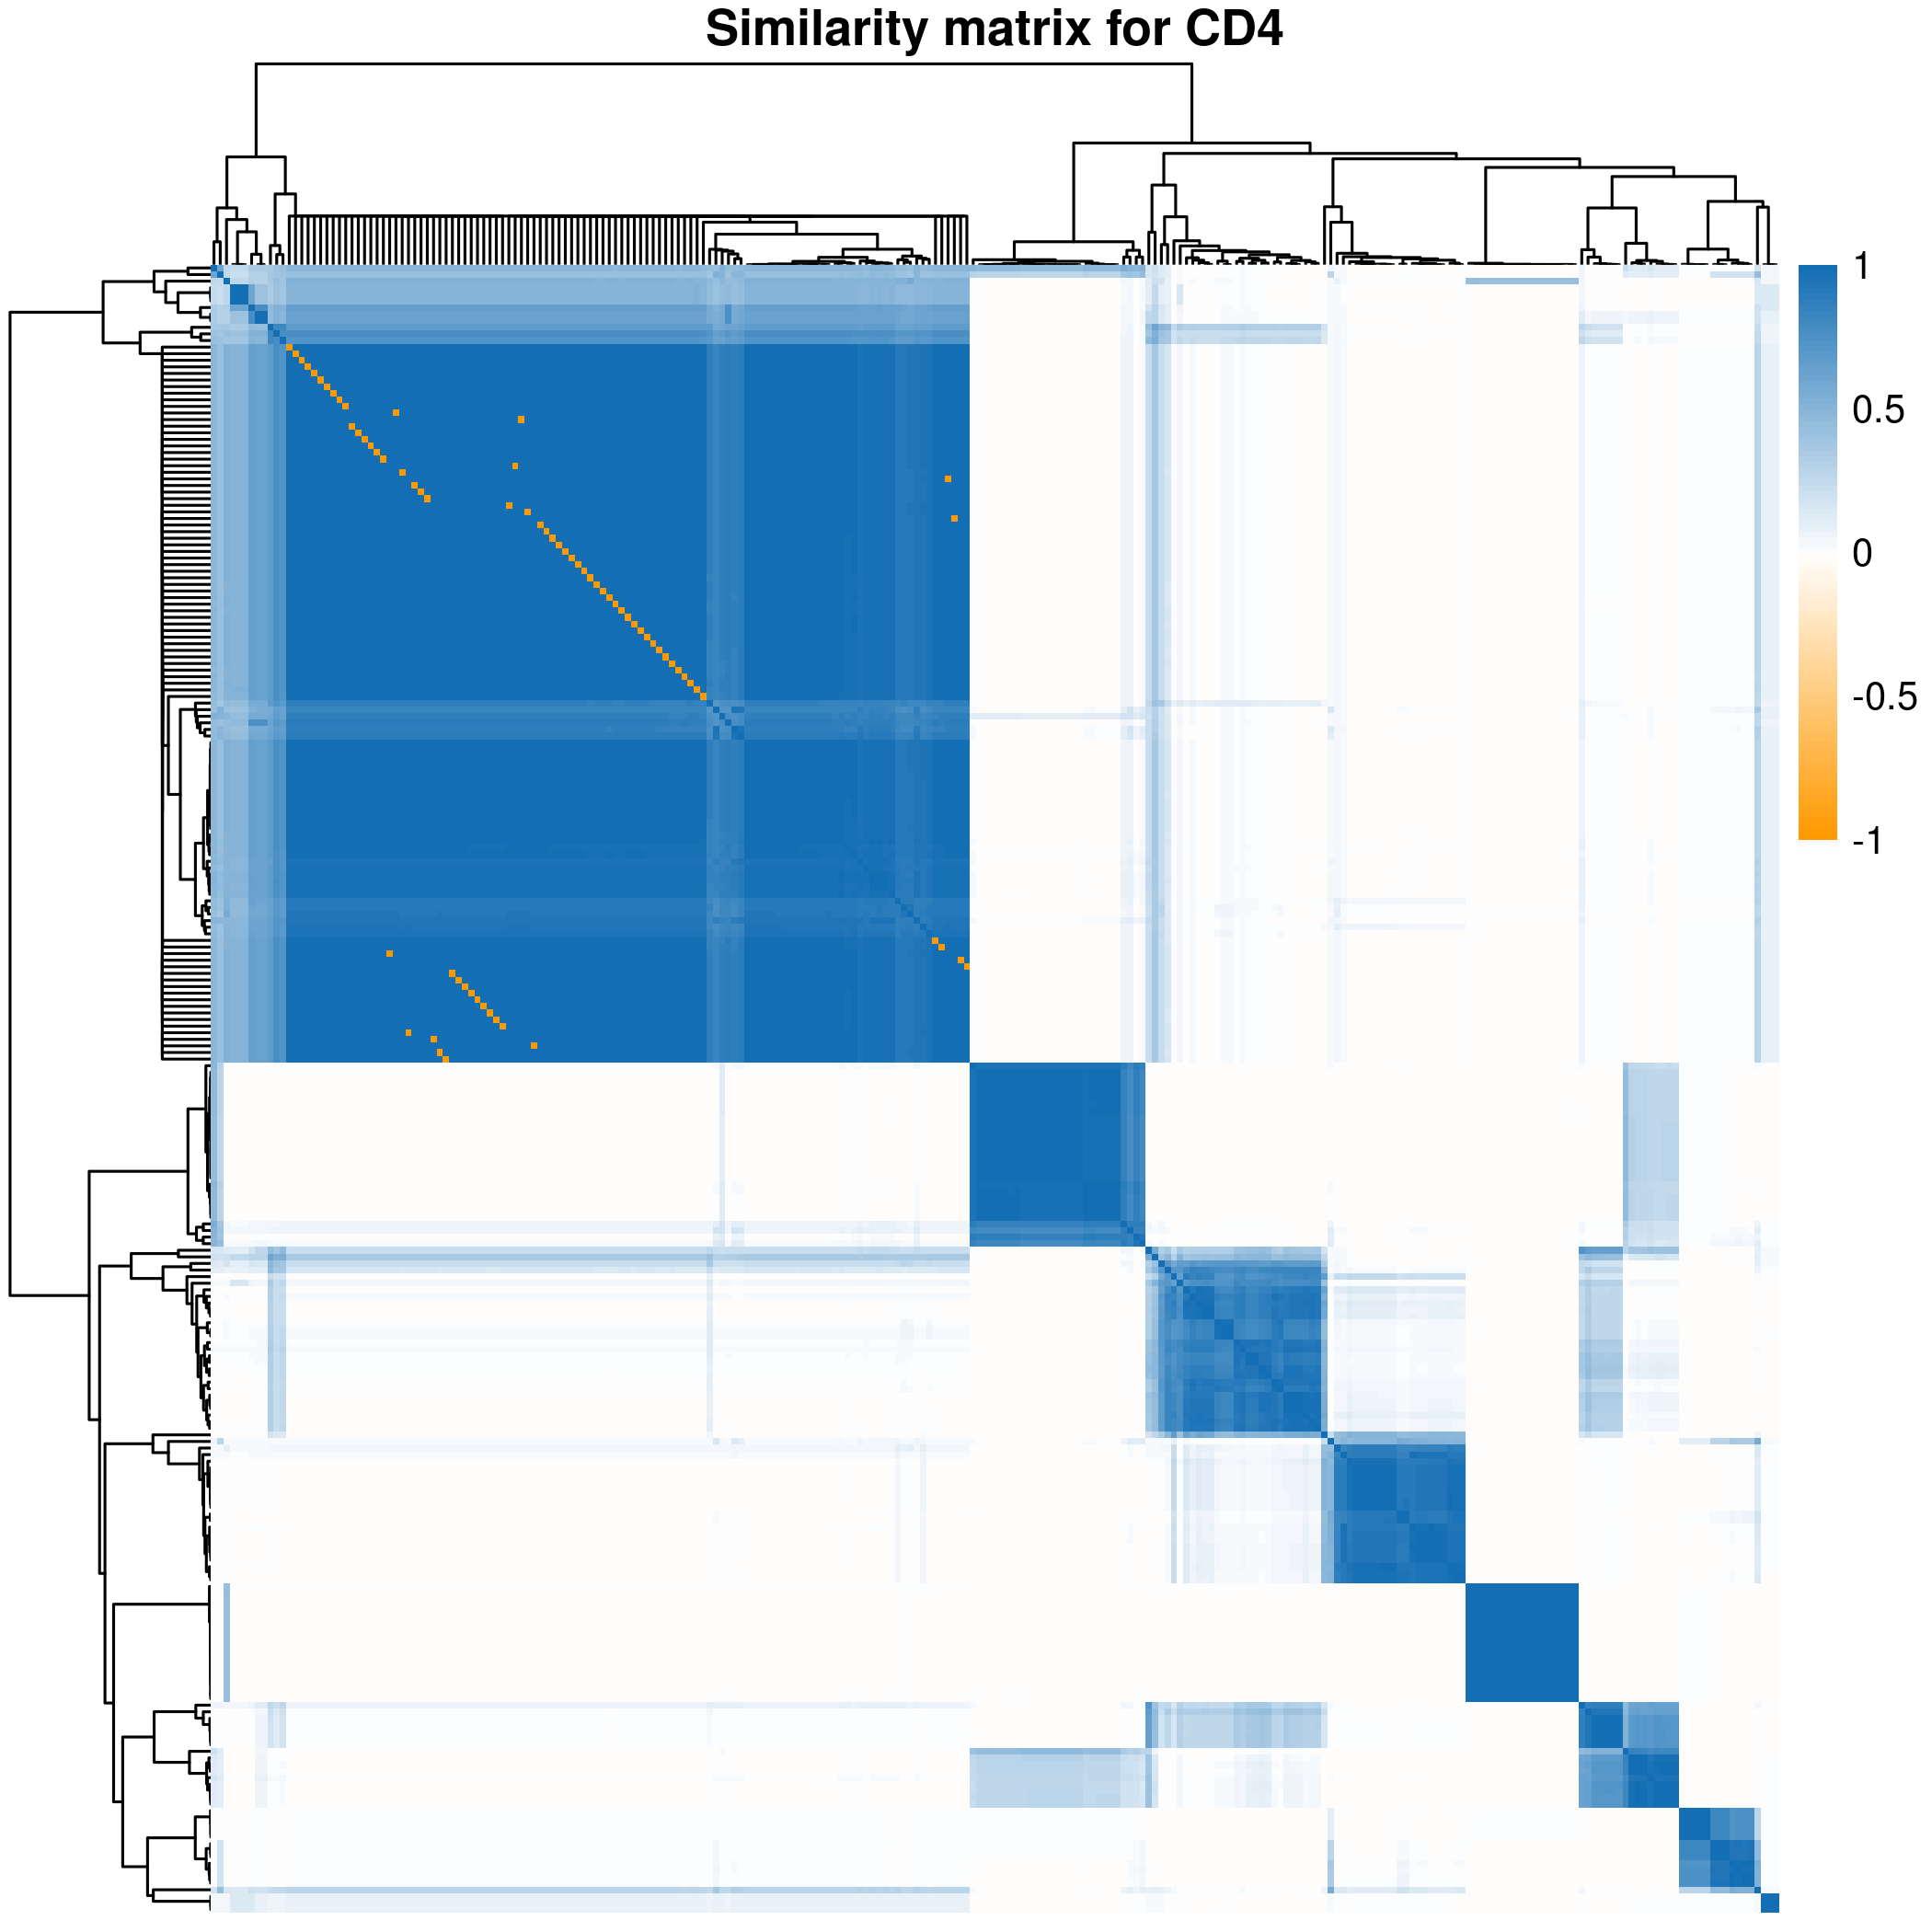
\includegraphics[scale=0.75]{Images/Biology_data/Set_250/All_datasets/Similarity_matrices/similarity_matrix_CD4.png}
		\caption{CEDAR Case 1: Heatmap of the PSM for the CD4 dataset from the consensus clustering of MDI.}
		\label{fig:results:cedar_1:mdi_cd4_psm}
	\end{figure}
	
	\newpage
	
	\begin{sidewaysfigure}[h]
		\centering
		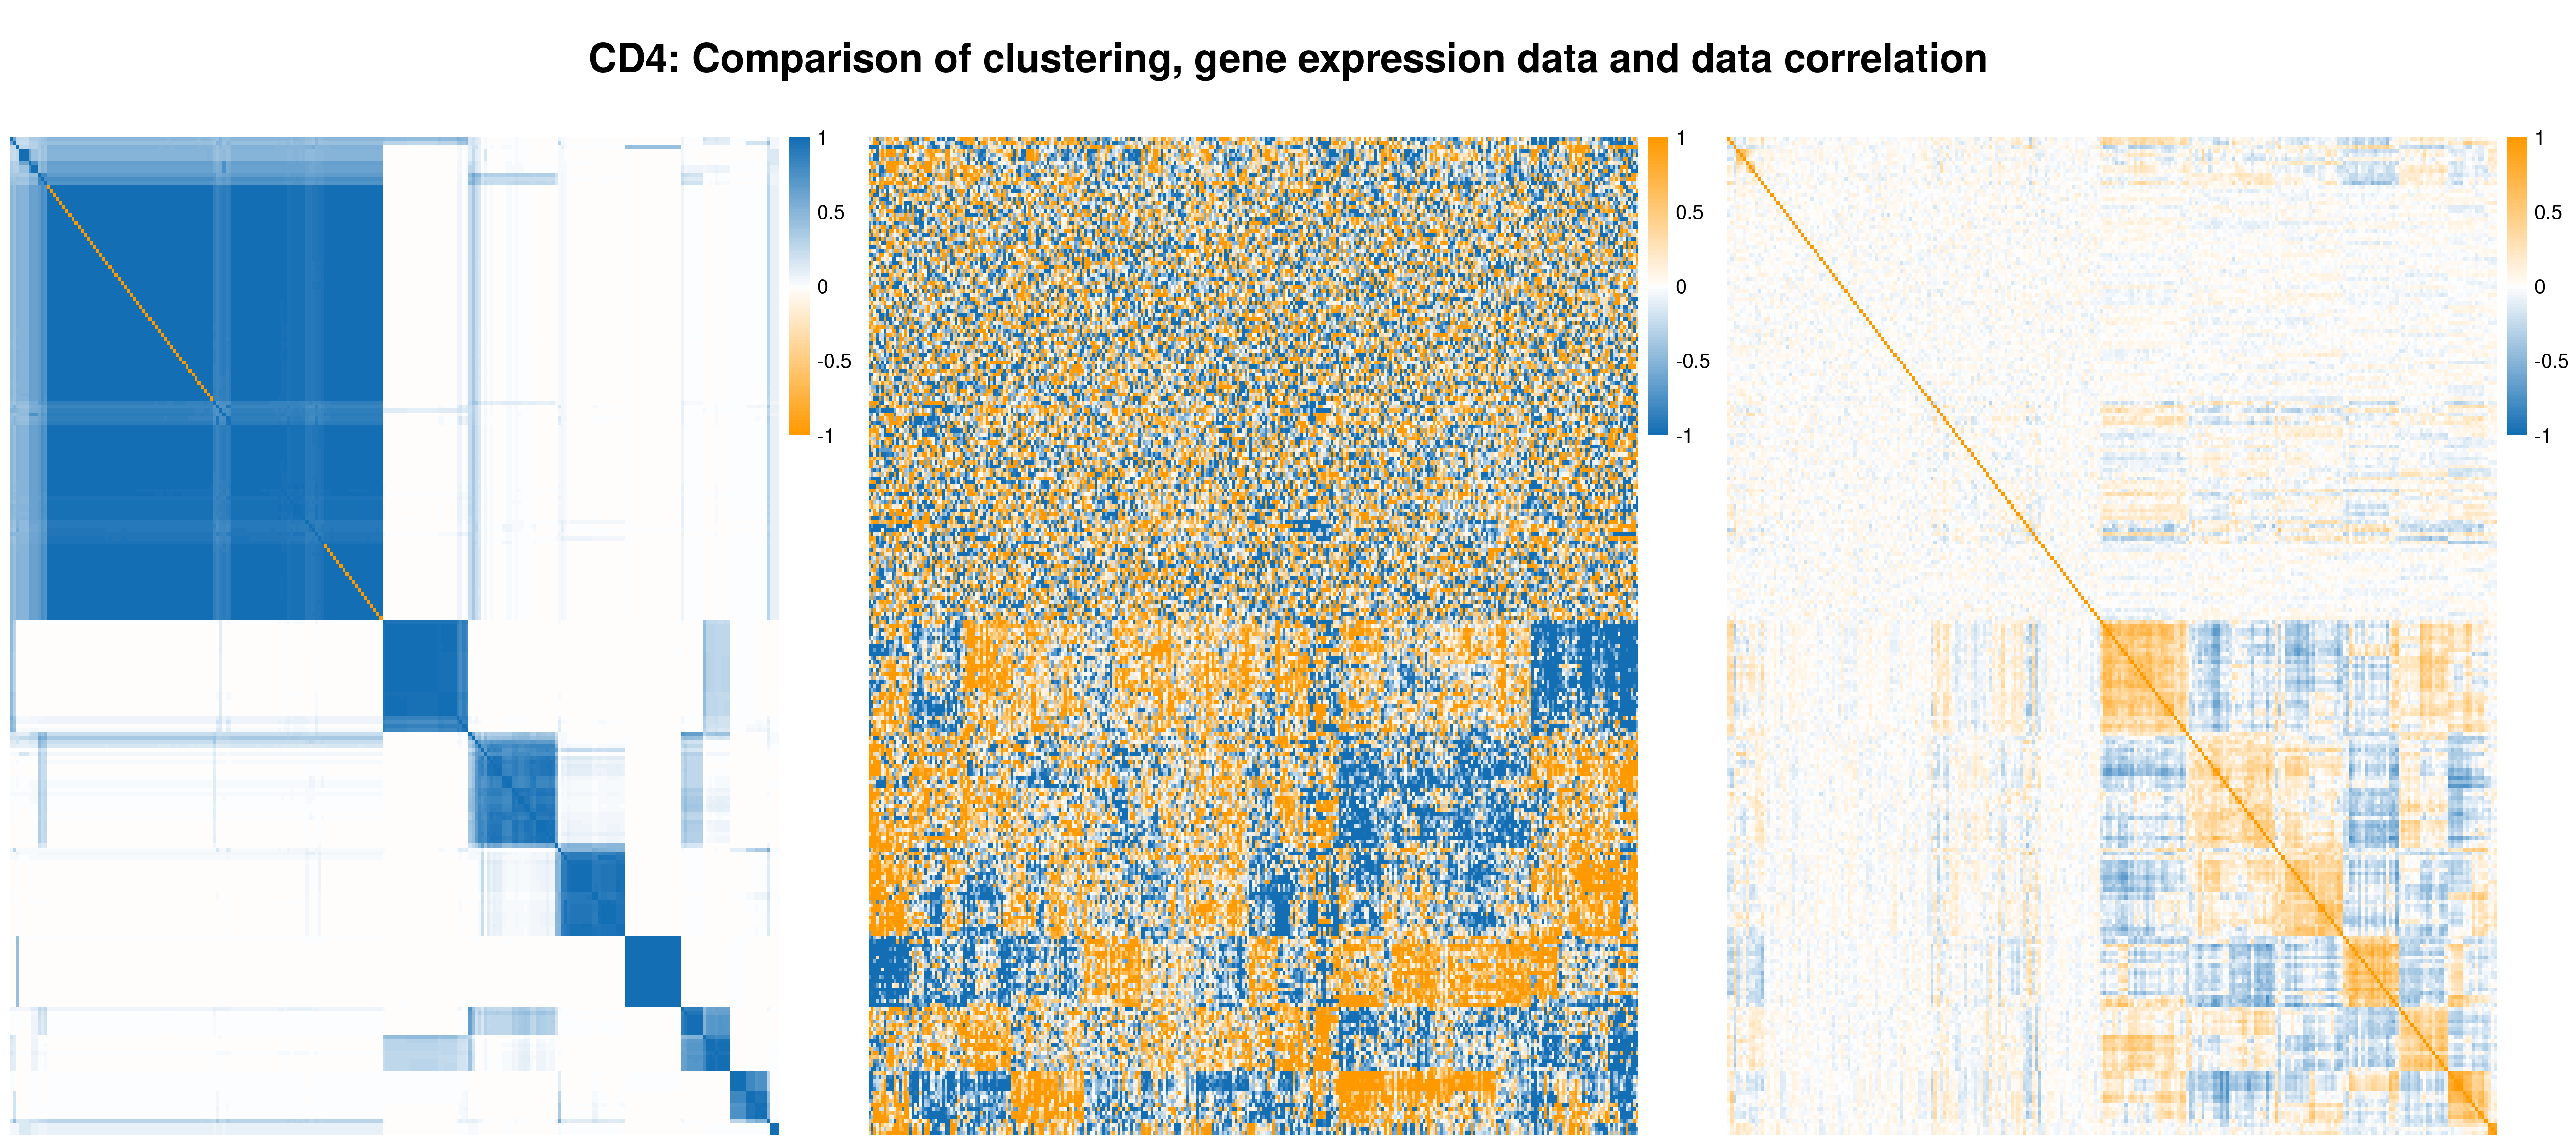
\includegraphics[scale=0.5]{Images/Biology_data/Set_250/All_datasets/Comparison_expression_clustering_correlation/CD4.png}
		\caption{CEDAR Case 1: Heatmap of the PSM for the CD4 dataset from the consensus clustering of MDI. The structure in the correlation matrix is uncovered by the PSM and one can see blocks within the standardised expression data which correspond to uncovered clusters in the PSM.}
		\label{fig:results:cedar_1:mdi_cd4_psm_expr_cor}
	\end{sidewaysfigure}

	\newpage
	
%	\begin{figure}[h]
%		\centering
%		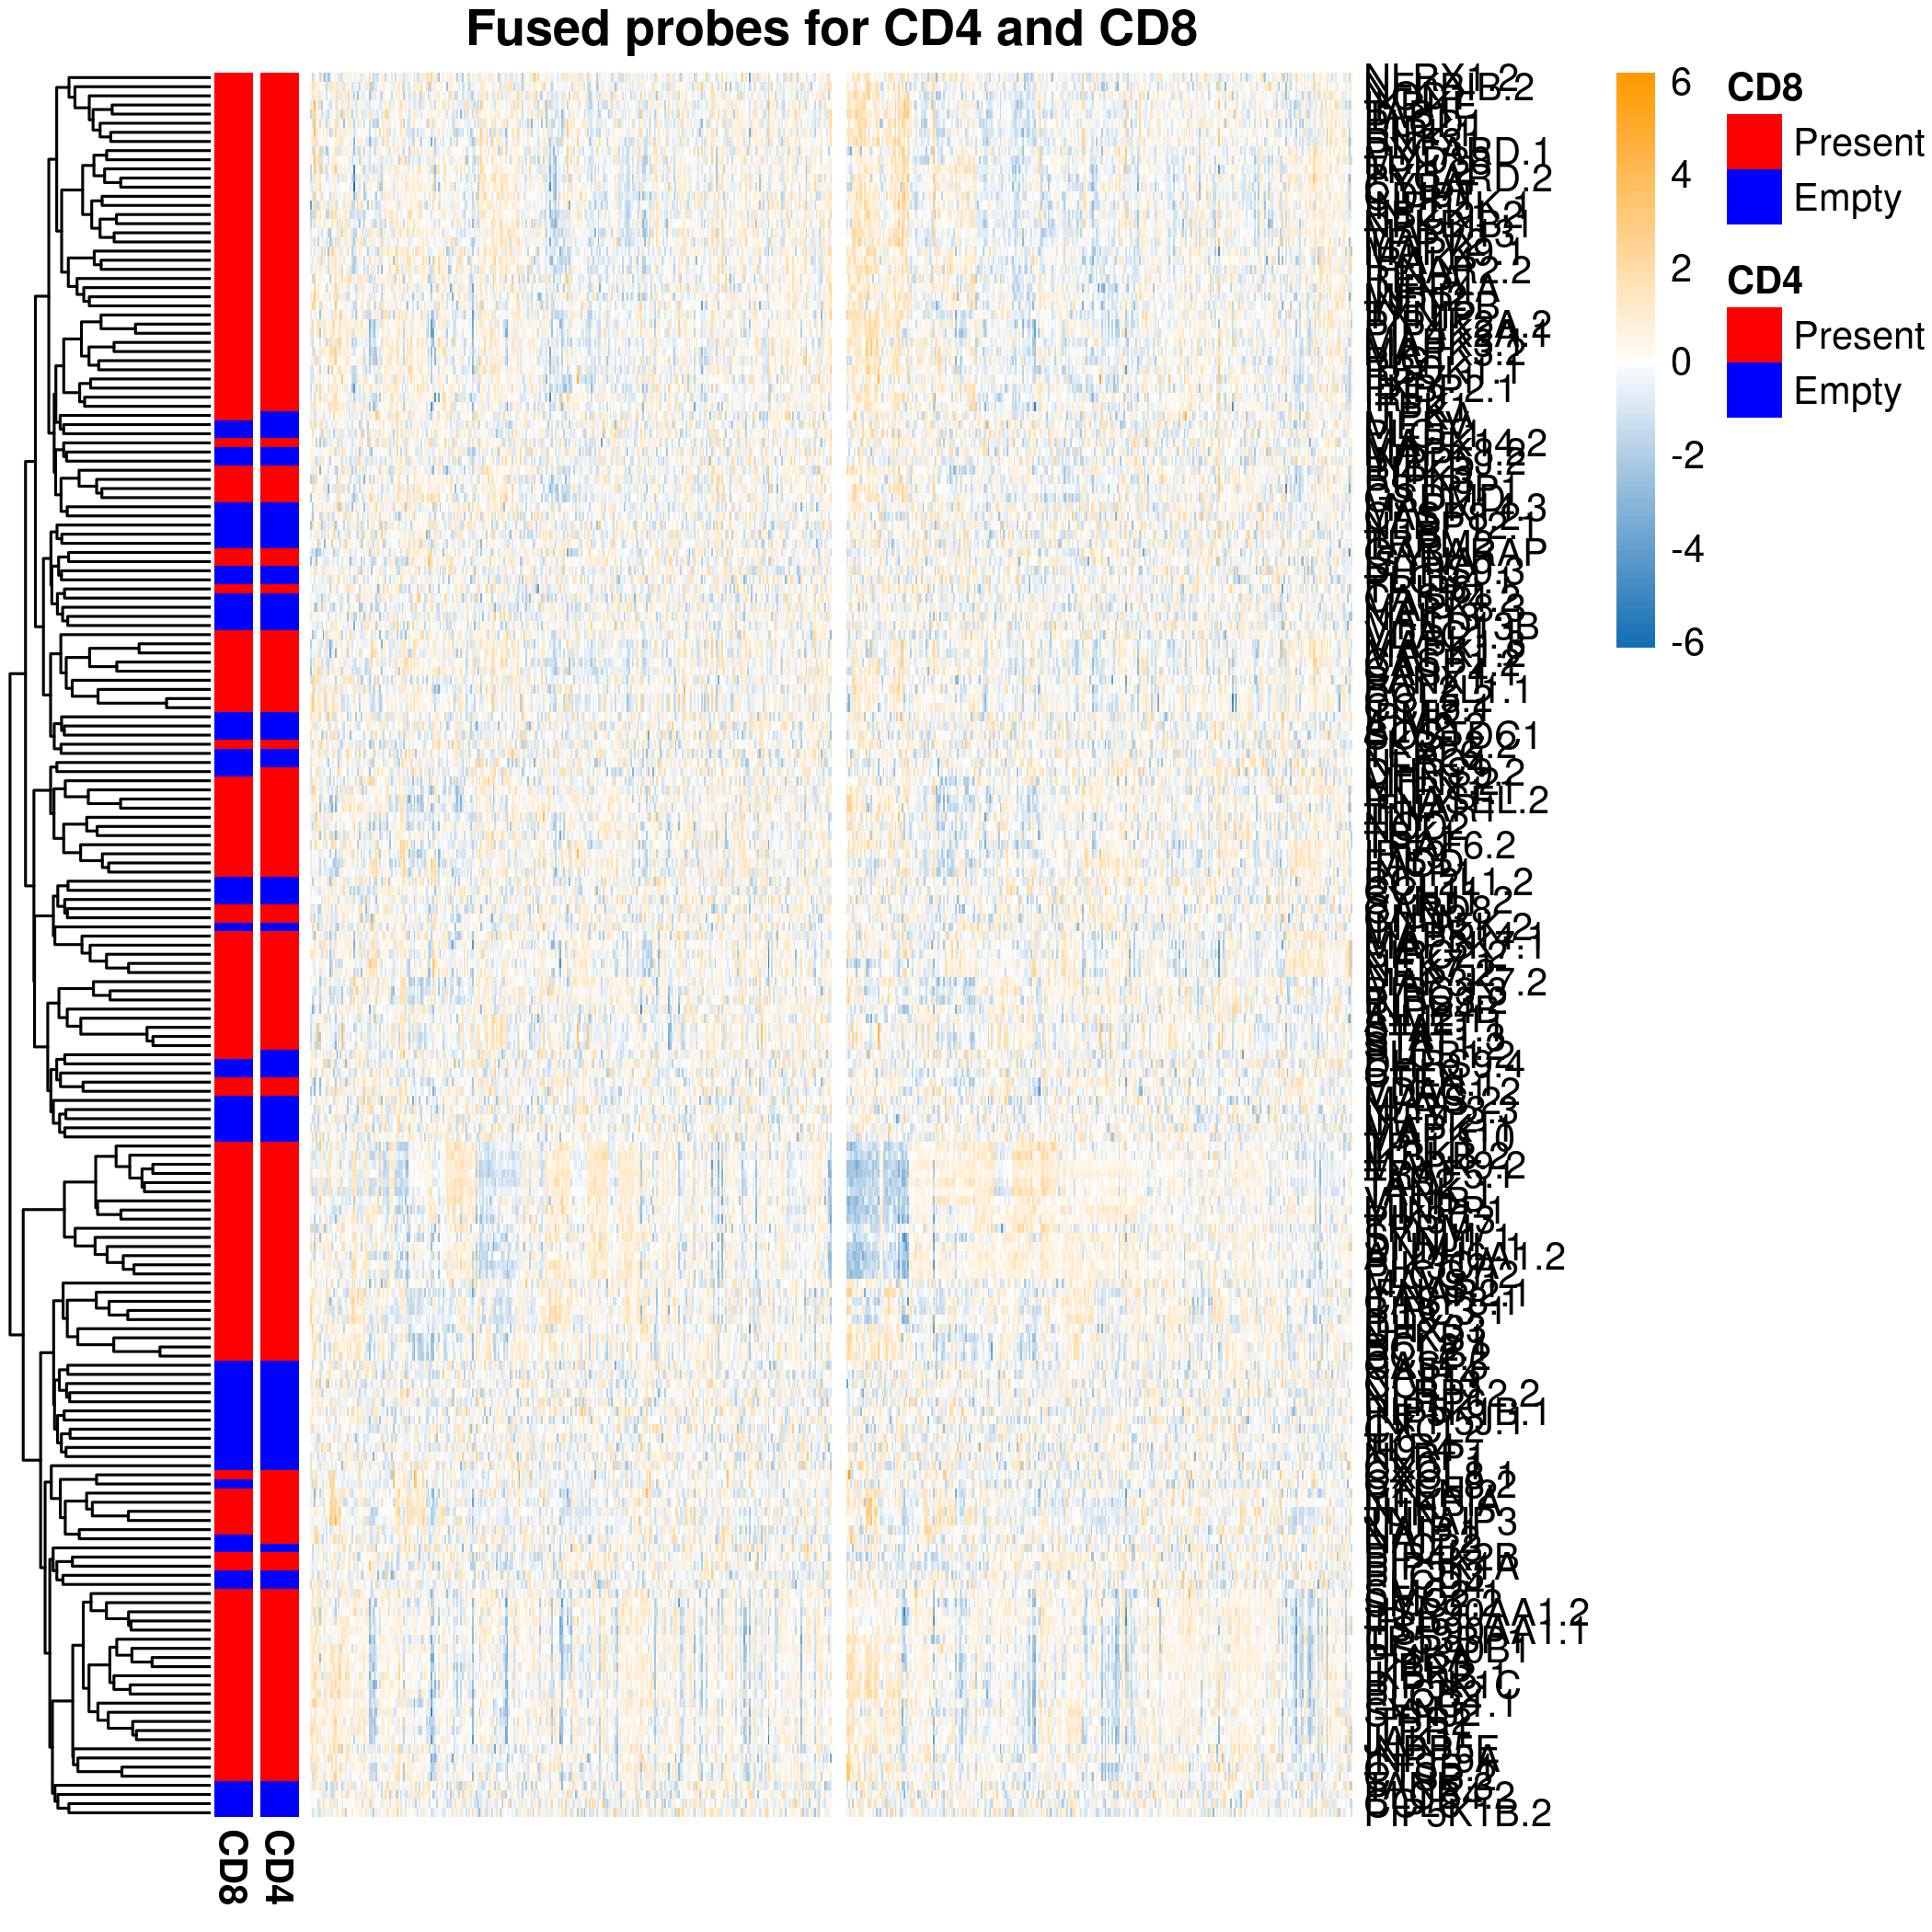
\includegraphics[scale=0.75]{Images/Biology_data/All_datasets/Fusion_expression_data/heatmap_fused_genes_CD4_CD8.png}
%		\caption{Heatmap of the expression data for the fused genes between the CD4 and CD8 datasets from the consensus clustering of MDI.}
%		\label{fig:mdi_cd4_cd8_fused_genes}
%	\end{figure}
%
%	\newpage
%
%	\begin{figure}[h]
%		\centering
%		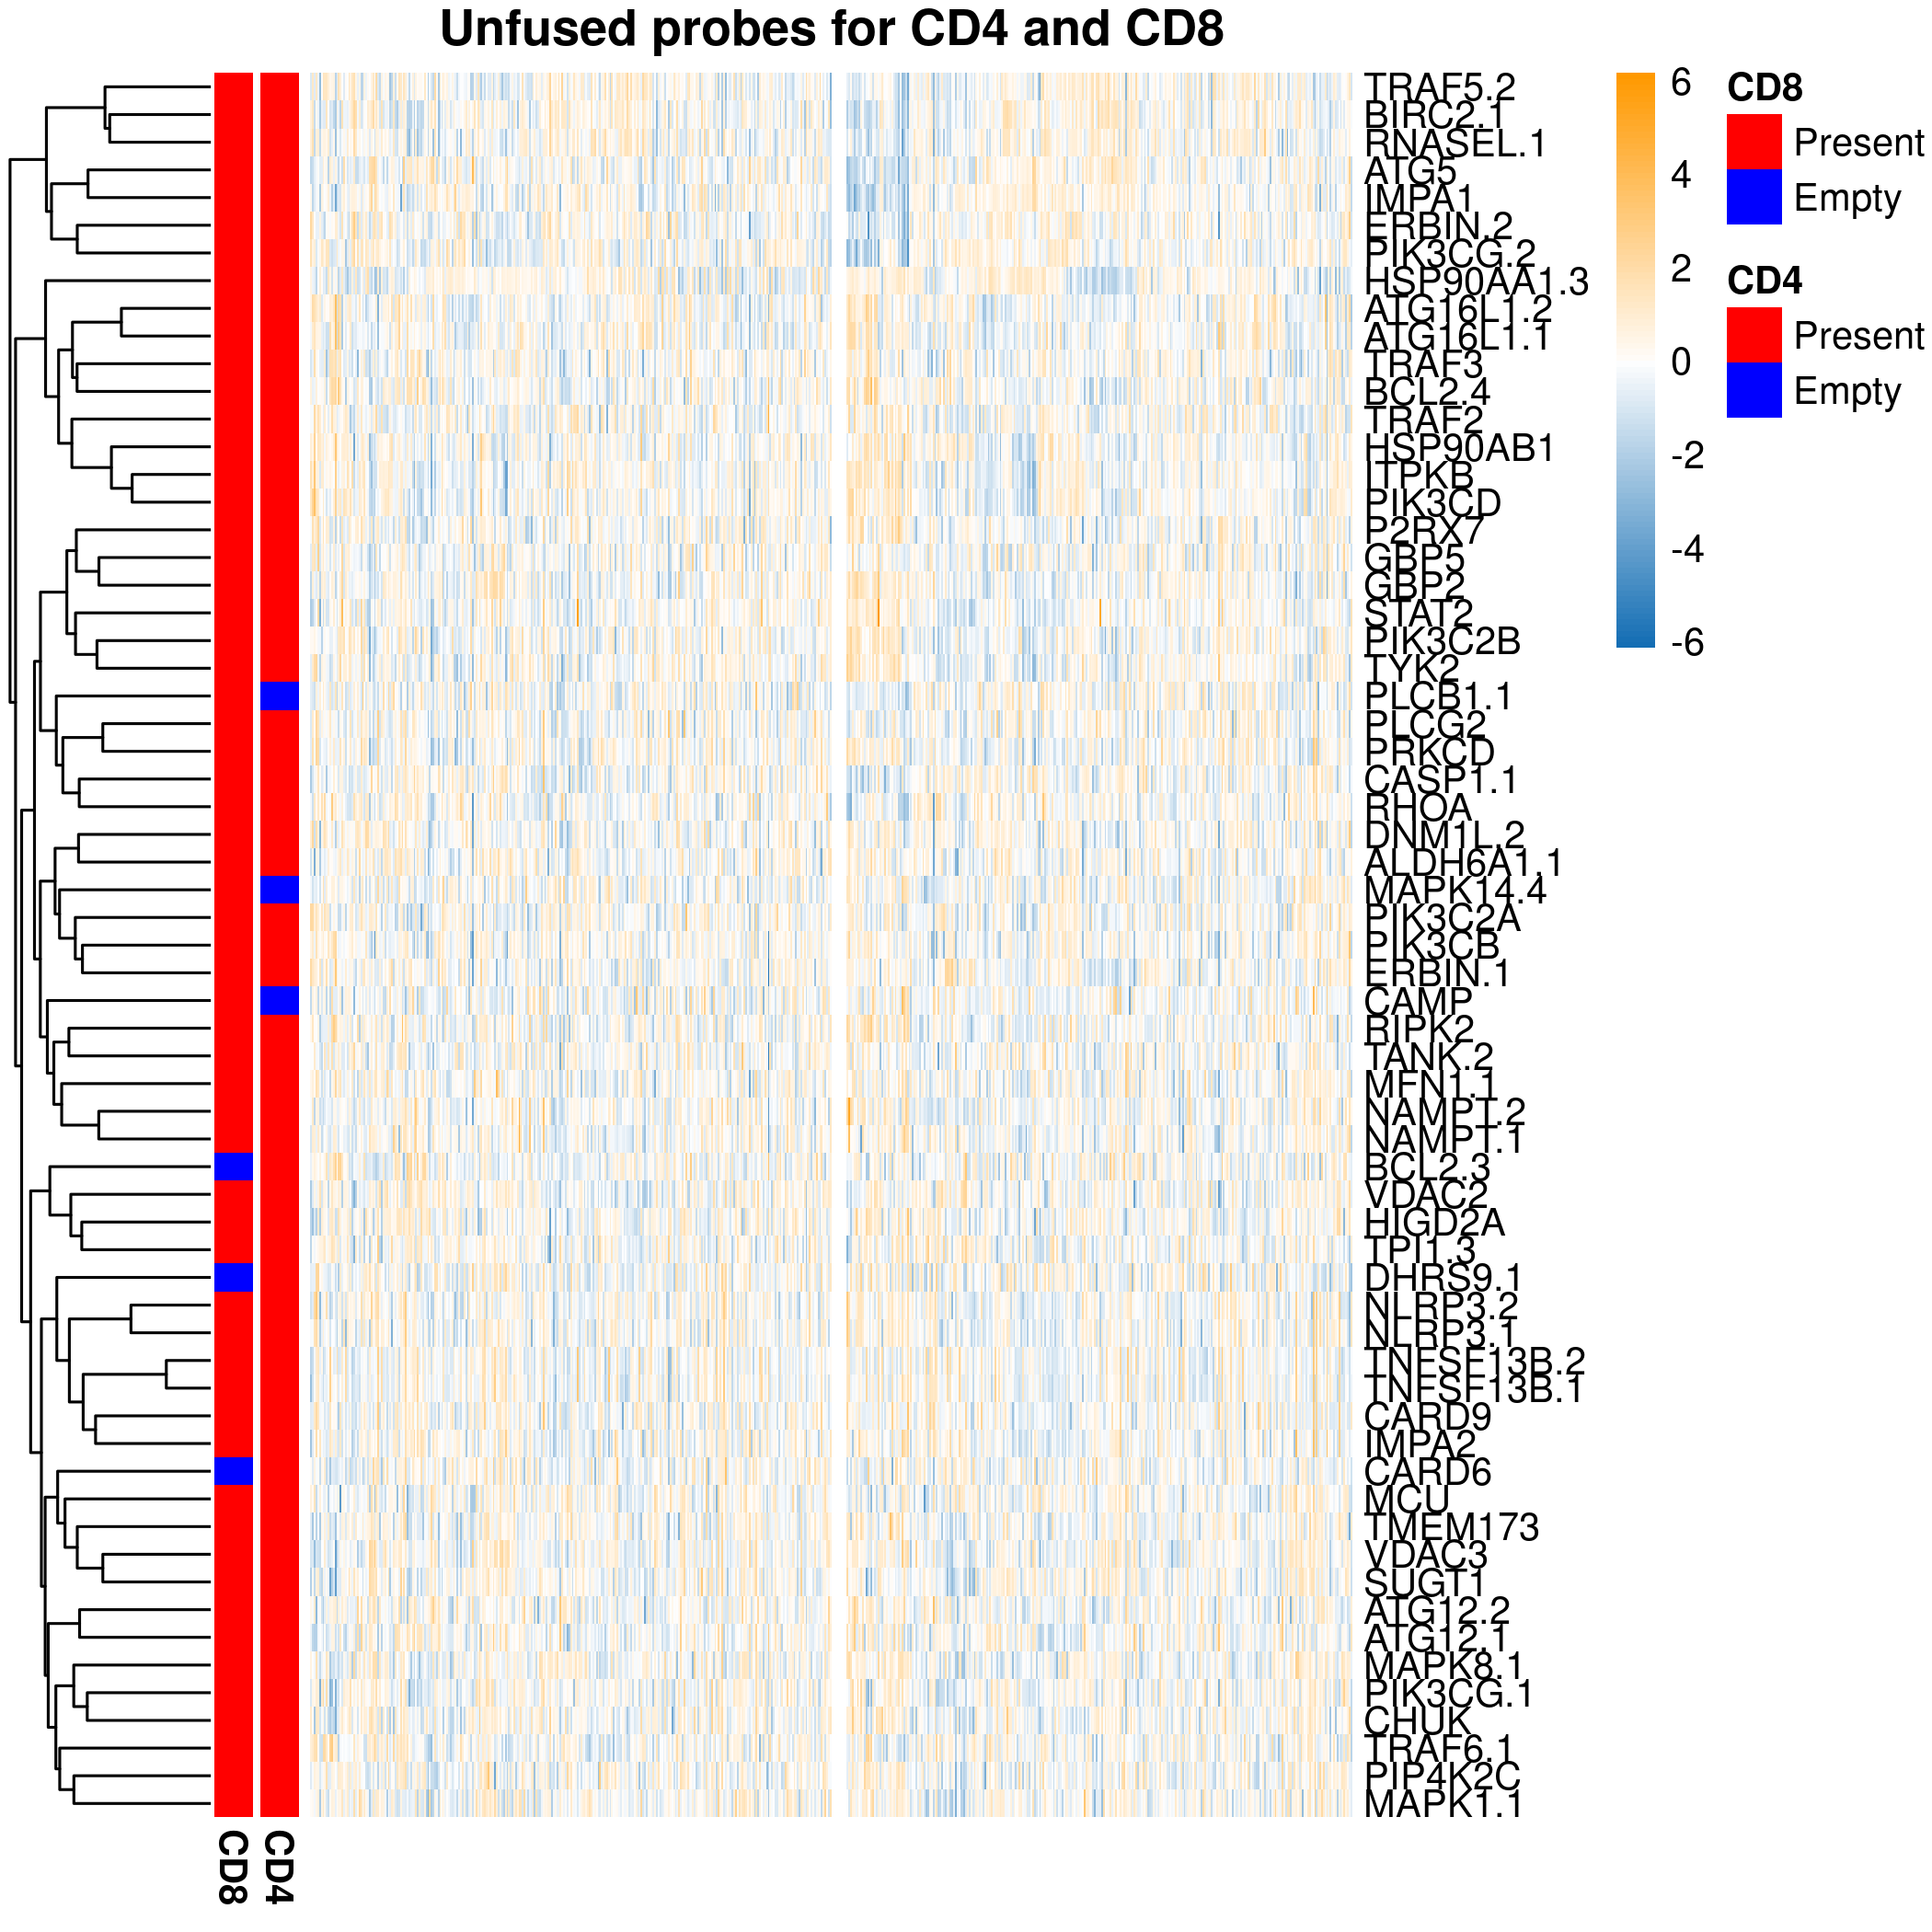
\includegraphics[scale=0.75]{Images/Biology_data/All_datasets/Fusion_expression_data/heatmap_unfused_genes_CD4_CD8.png}
%		\caption{Heatmap of the expression data for the unfused genes between the CD4 and CD8 datasets from the consensus clustering of MDI.}
%		\label{fig:mdi_cd4_cd8_unfused_genes}
%	\end{figure}
		
	\newpage
	
%	The clustering for the KEGG pathway was inspected using three visualisation techniques:
	\begin{enumerate}
		\item In figure \ref{fig:results:cedar_1:mdi_cd4_inostiol_psm_cor} one can see that a number of sub-clusters are found by the consensus clustering within the Inositol pathway, with some members not allocated to the same cluster as any other member with any certainty. This might be expected due to the diversity of purpose that members of the Inositol pathway have \citep{monserrate2010inositol}.
		\item Figures \ref{fig:results:cedar_1:mdi_cd4_inostiol_alignemnt_prob_distn}, \ref{fig:results:cedar_1:mdi_cd8_inostiol_alignemnt_prob_distn} and \ref{fig:results:cedar_1:mdi_il_inostiol_alignemnt_prob_distn} show that the clustering of the Inositol probes within the PSM is more than structured than would expect for a random set of the same size. Furthermore, the level of structure varies across datasets but there appears to be some signal for this pathway in each dataset.
		\item Figure \ref{fig:results:cedar_1:mdi_cd4_inostiol_psm_violin} shows that the PSM for the Inositol probes does have a entries that are slightly higher than the PSM entries for all other probes.
	\end{enumerate}
	
%		\newpage
	
	\begin{sidewaysfigure}[h]
		\centering
		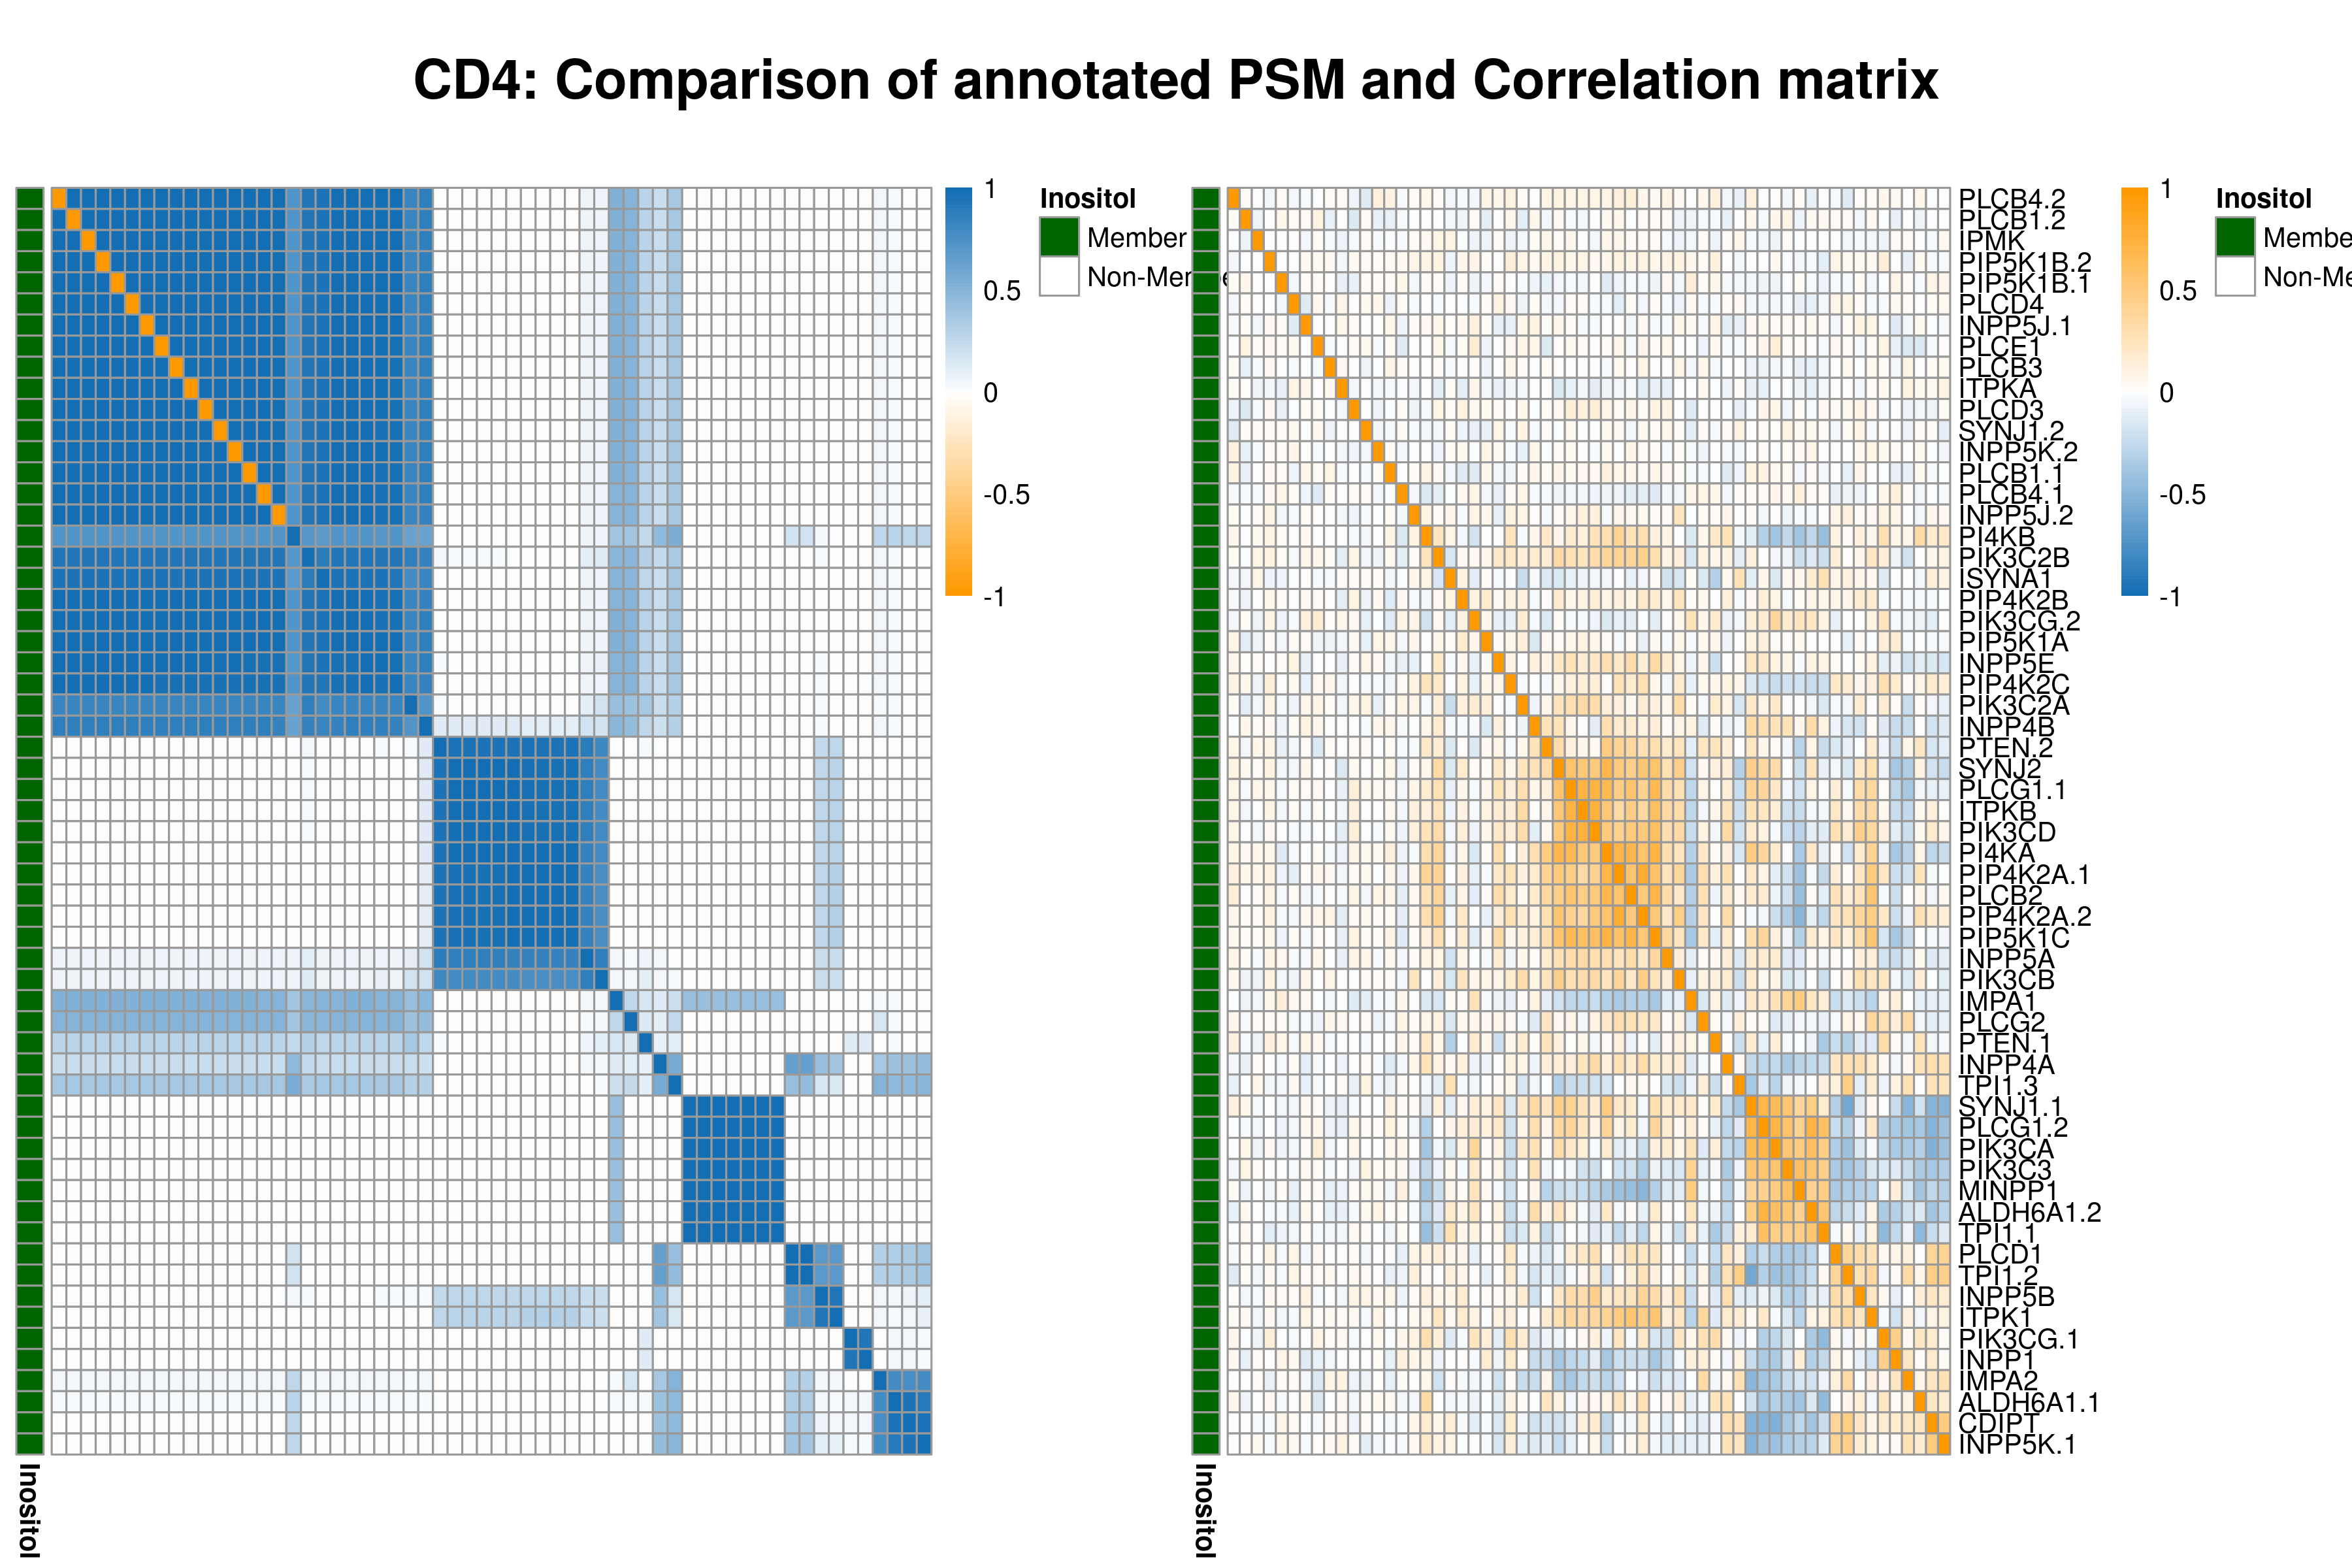
\includegraphics[scale=0.75]{Images/Biology_data/Set_250/All_datasets/Heatmaps/KEGG_INOSITOL_PHOSPHATE_METABOLISM/CD4_comp_psm_corr.png}
		\caption{CEDAR Case 1: Heatmap of the PSM and expression data for the Inositol genes for the CD4 datasets from the consensus clustering of MDI. One can see that a number of sub-clusters are present as might be expected due to the diversity of purpose that members of the Inositol pathway have \citep{monserrate2010inositol}.}
		\label{fig:results:cedar_1:mdi_cd4_inostiol_psm_cor}
	\end{sidewaysfigure}


	\begin{figure}[h]
		\centering
		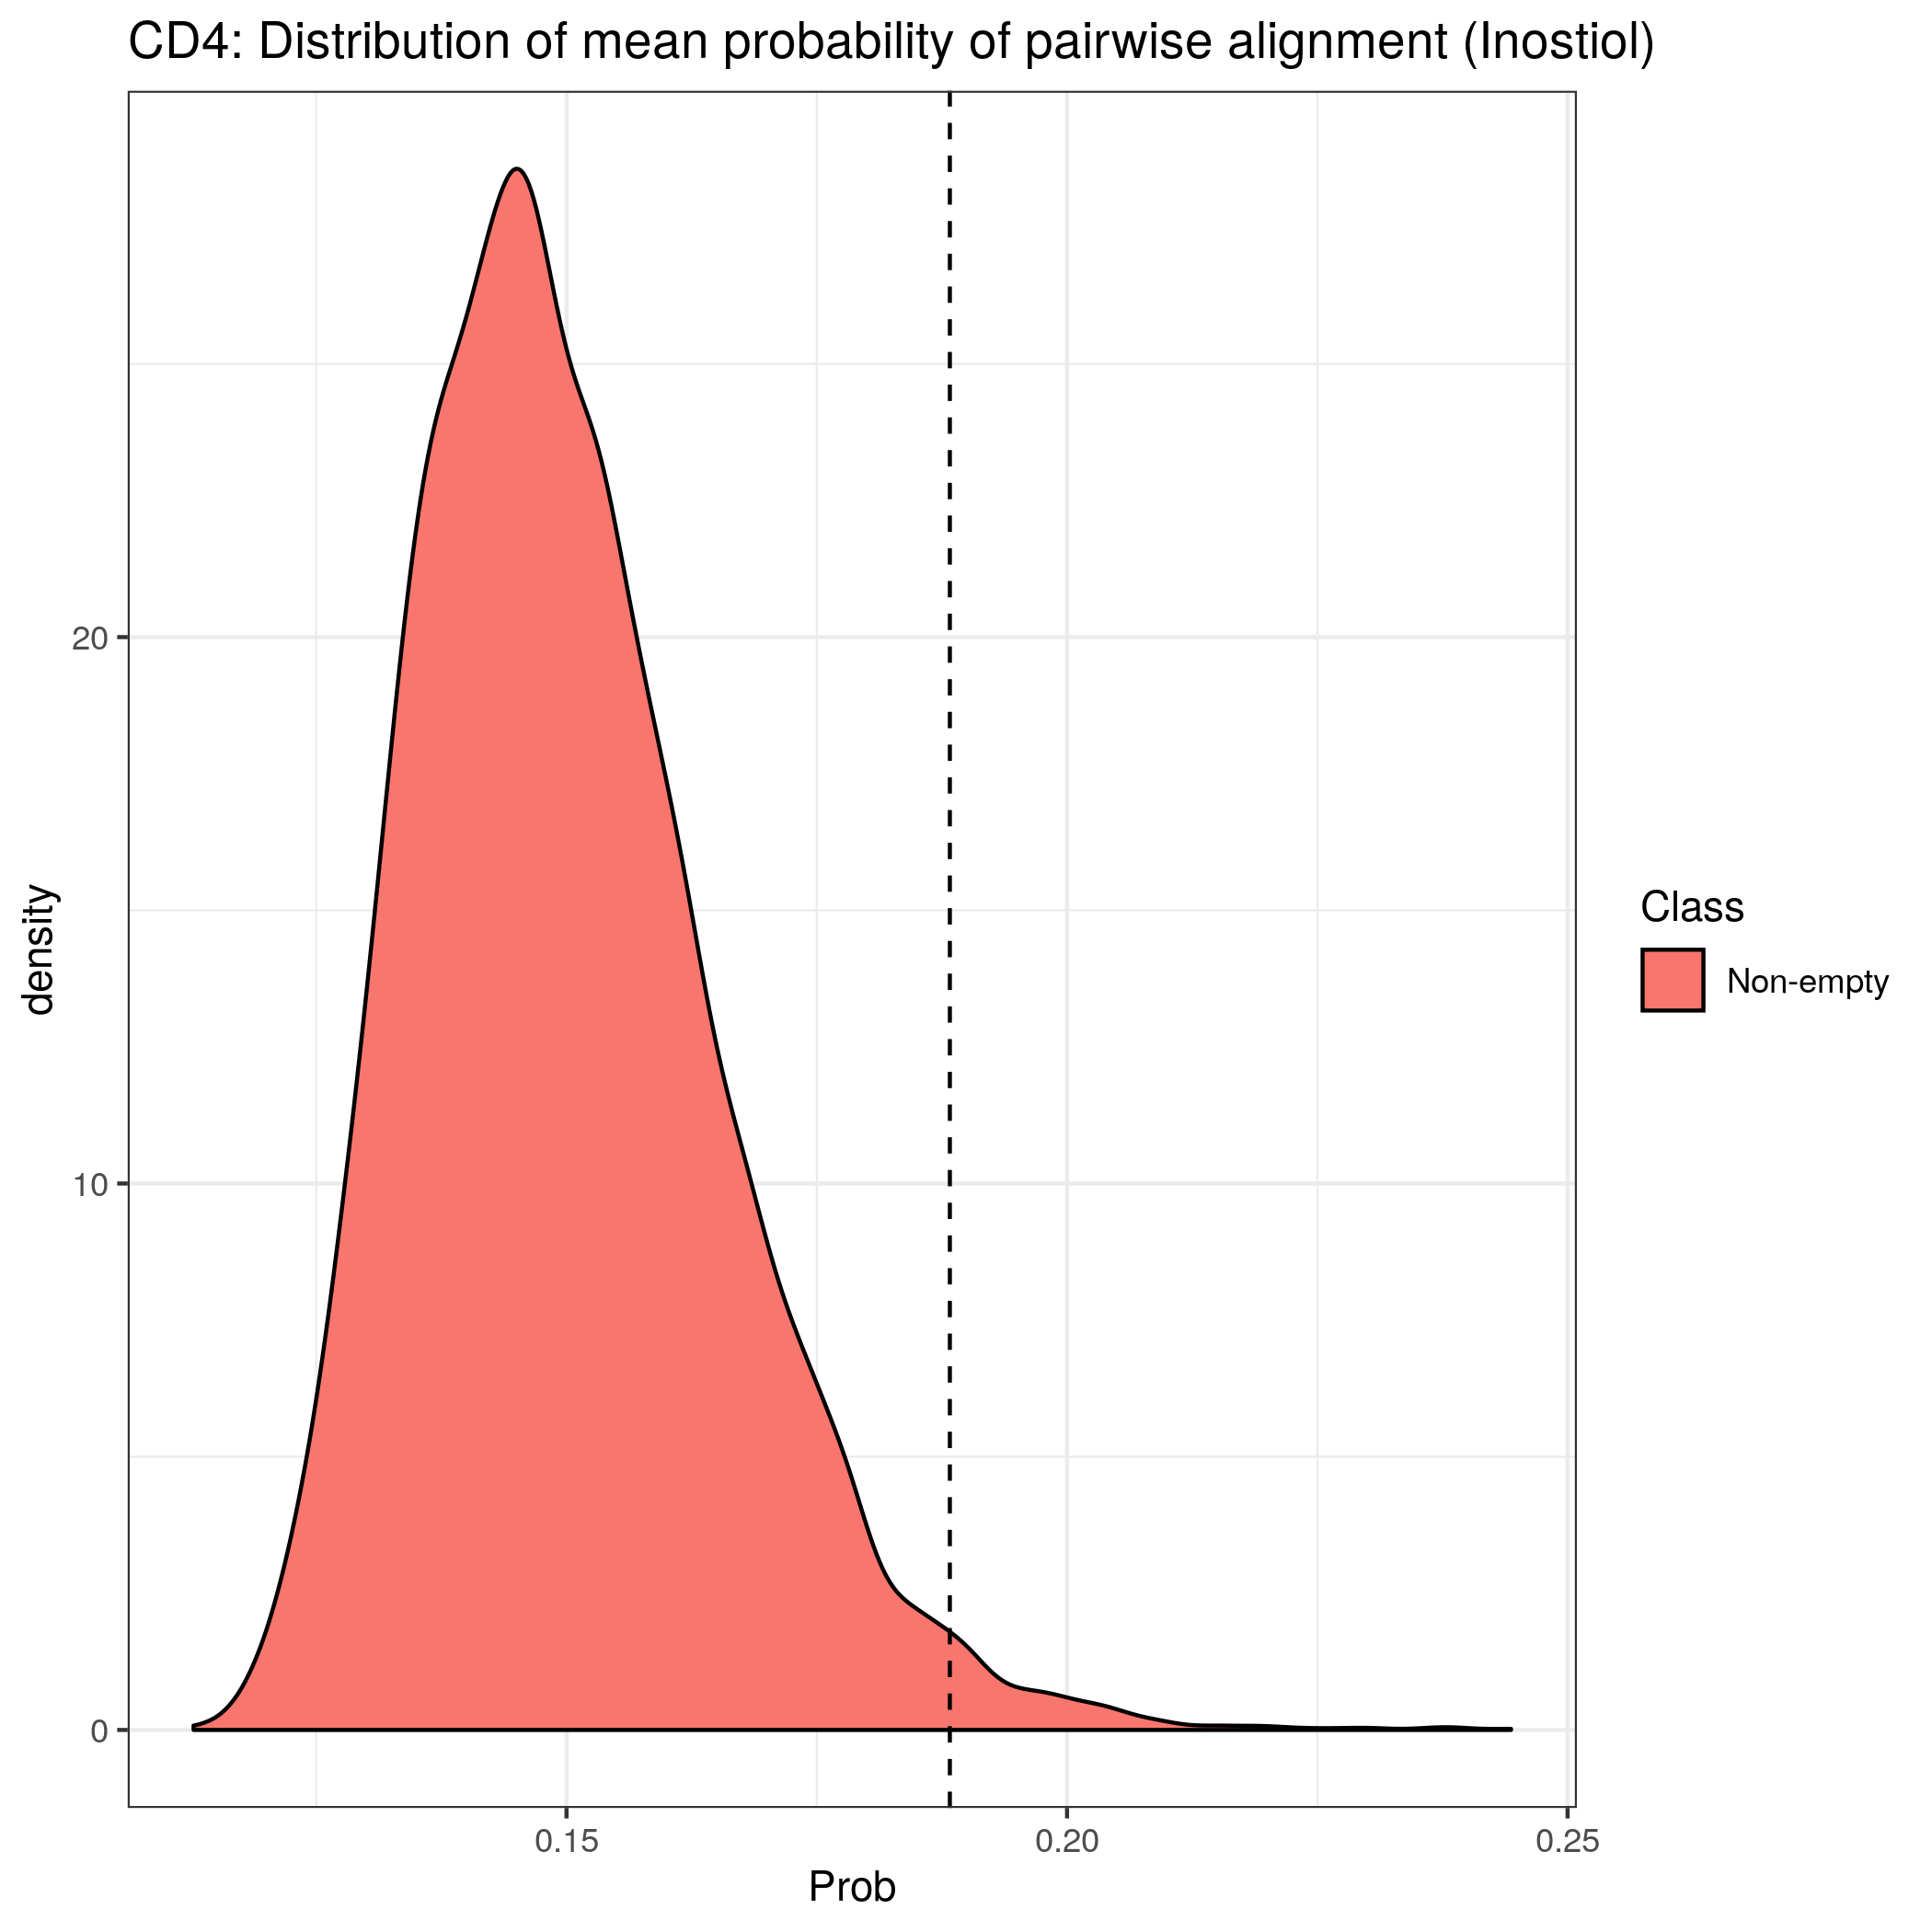
\includegraphics[scale=0.75]{Images/Biology_data/Set_250/All_datasets/Mean_alignment_probability/CD4_KEGG_INOSITOL_PHOSPHATE_METABOLISM.png}
		\caption{CEDAR Case 1: Plot of the distribution of the mean probability of pairwise alignment for a random sample of 60 genes (to coincide with the number of genes associated with the Inositol pathway present) with a dashed line indicating the mean probability of pairwise alignment for the Inositol genes in the CD4 dataset for the 250 probe set.}
		\label{fig:results:cedar_1:mdi_cd4_inostiol_alignemnt_prob_distn}
	\end{figure}

	\begin{figure}[h]
		\centering
		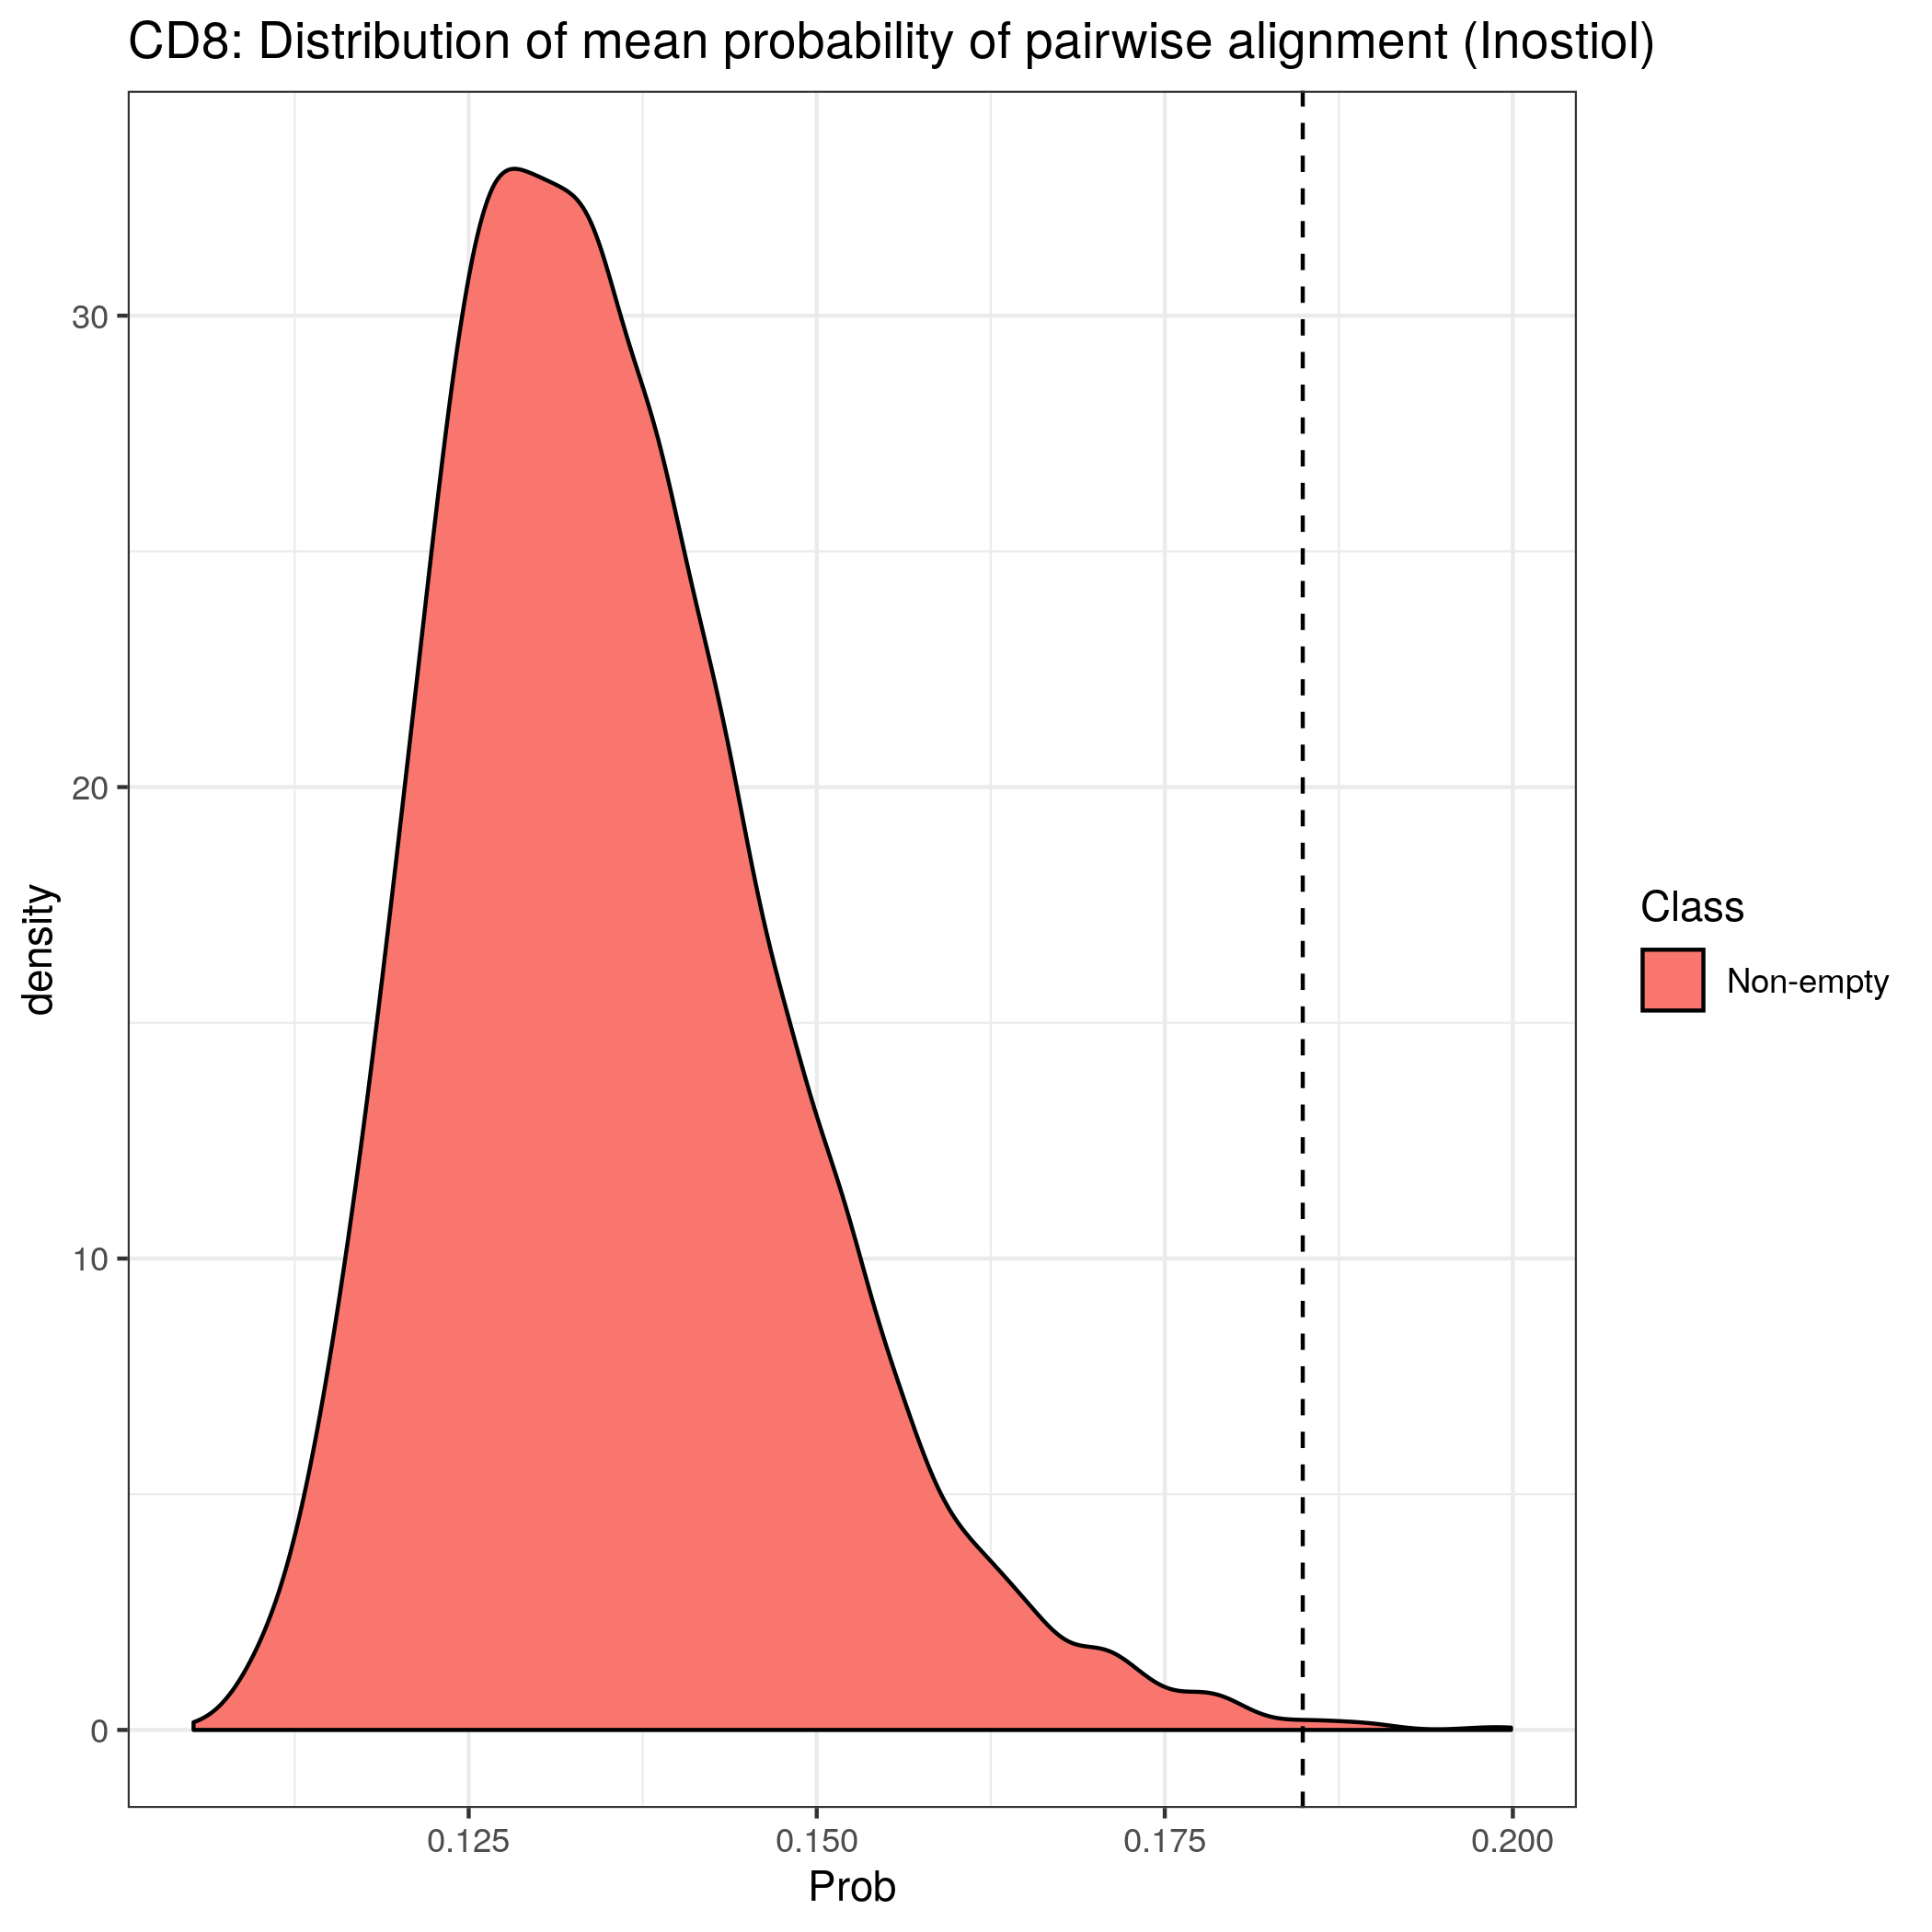
\includegraphics[scale=0.75]{Images/Biology_data/Set_250/All_datasets/Mean_alignment_probability/CD8_KEGG_INOSITOL_PHOSPHATE_METABOLISM.png}
		\caption{CEDAR Case 1: Plot of the distribution of the mean probability of pairwise alignment for a random sample of 60 genes with a dashed line indicating the mean probability of pairwise alignment for the Inositol genes in the CD8 dataset for the 250 probe set.}
		\label{fig:results:cedar_1:mdi_cd8_inostiol_alignemnt_prob_distn}
	\end{figure}

	\begin{figure}[h]
		\centering
		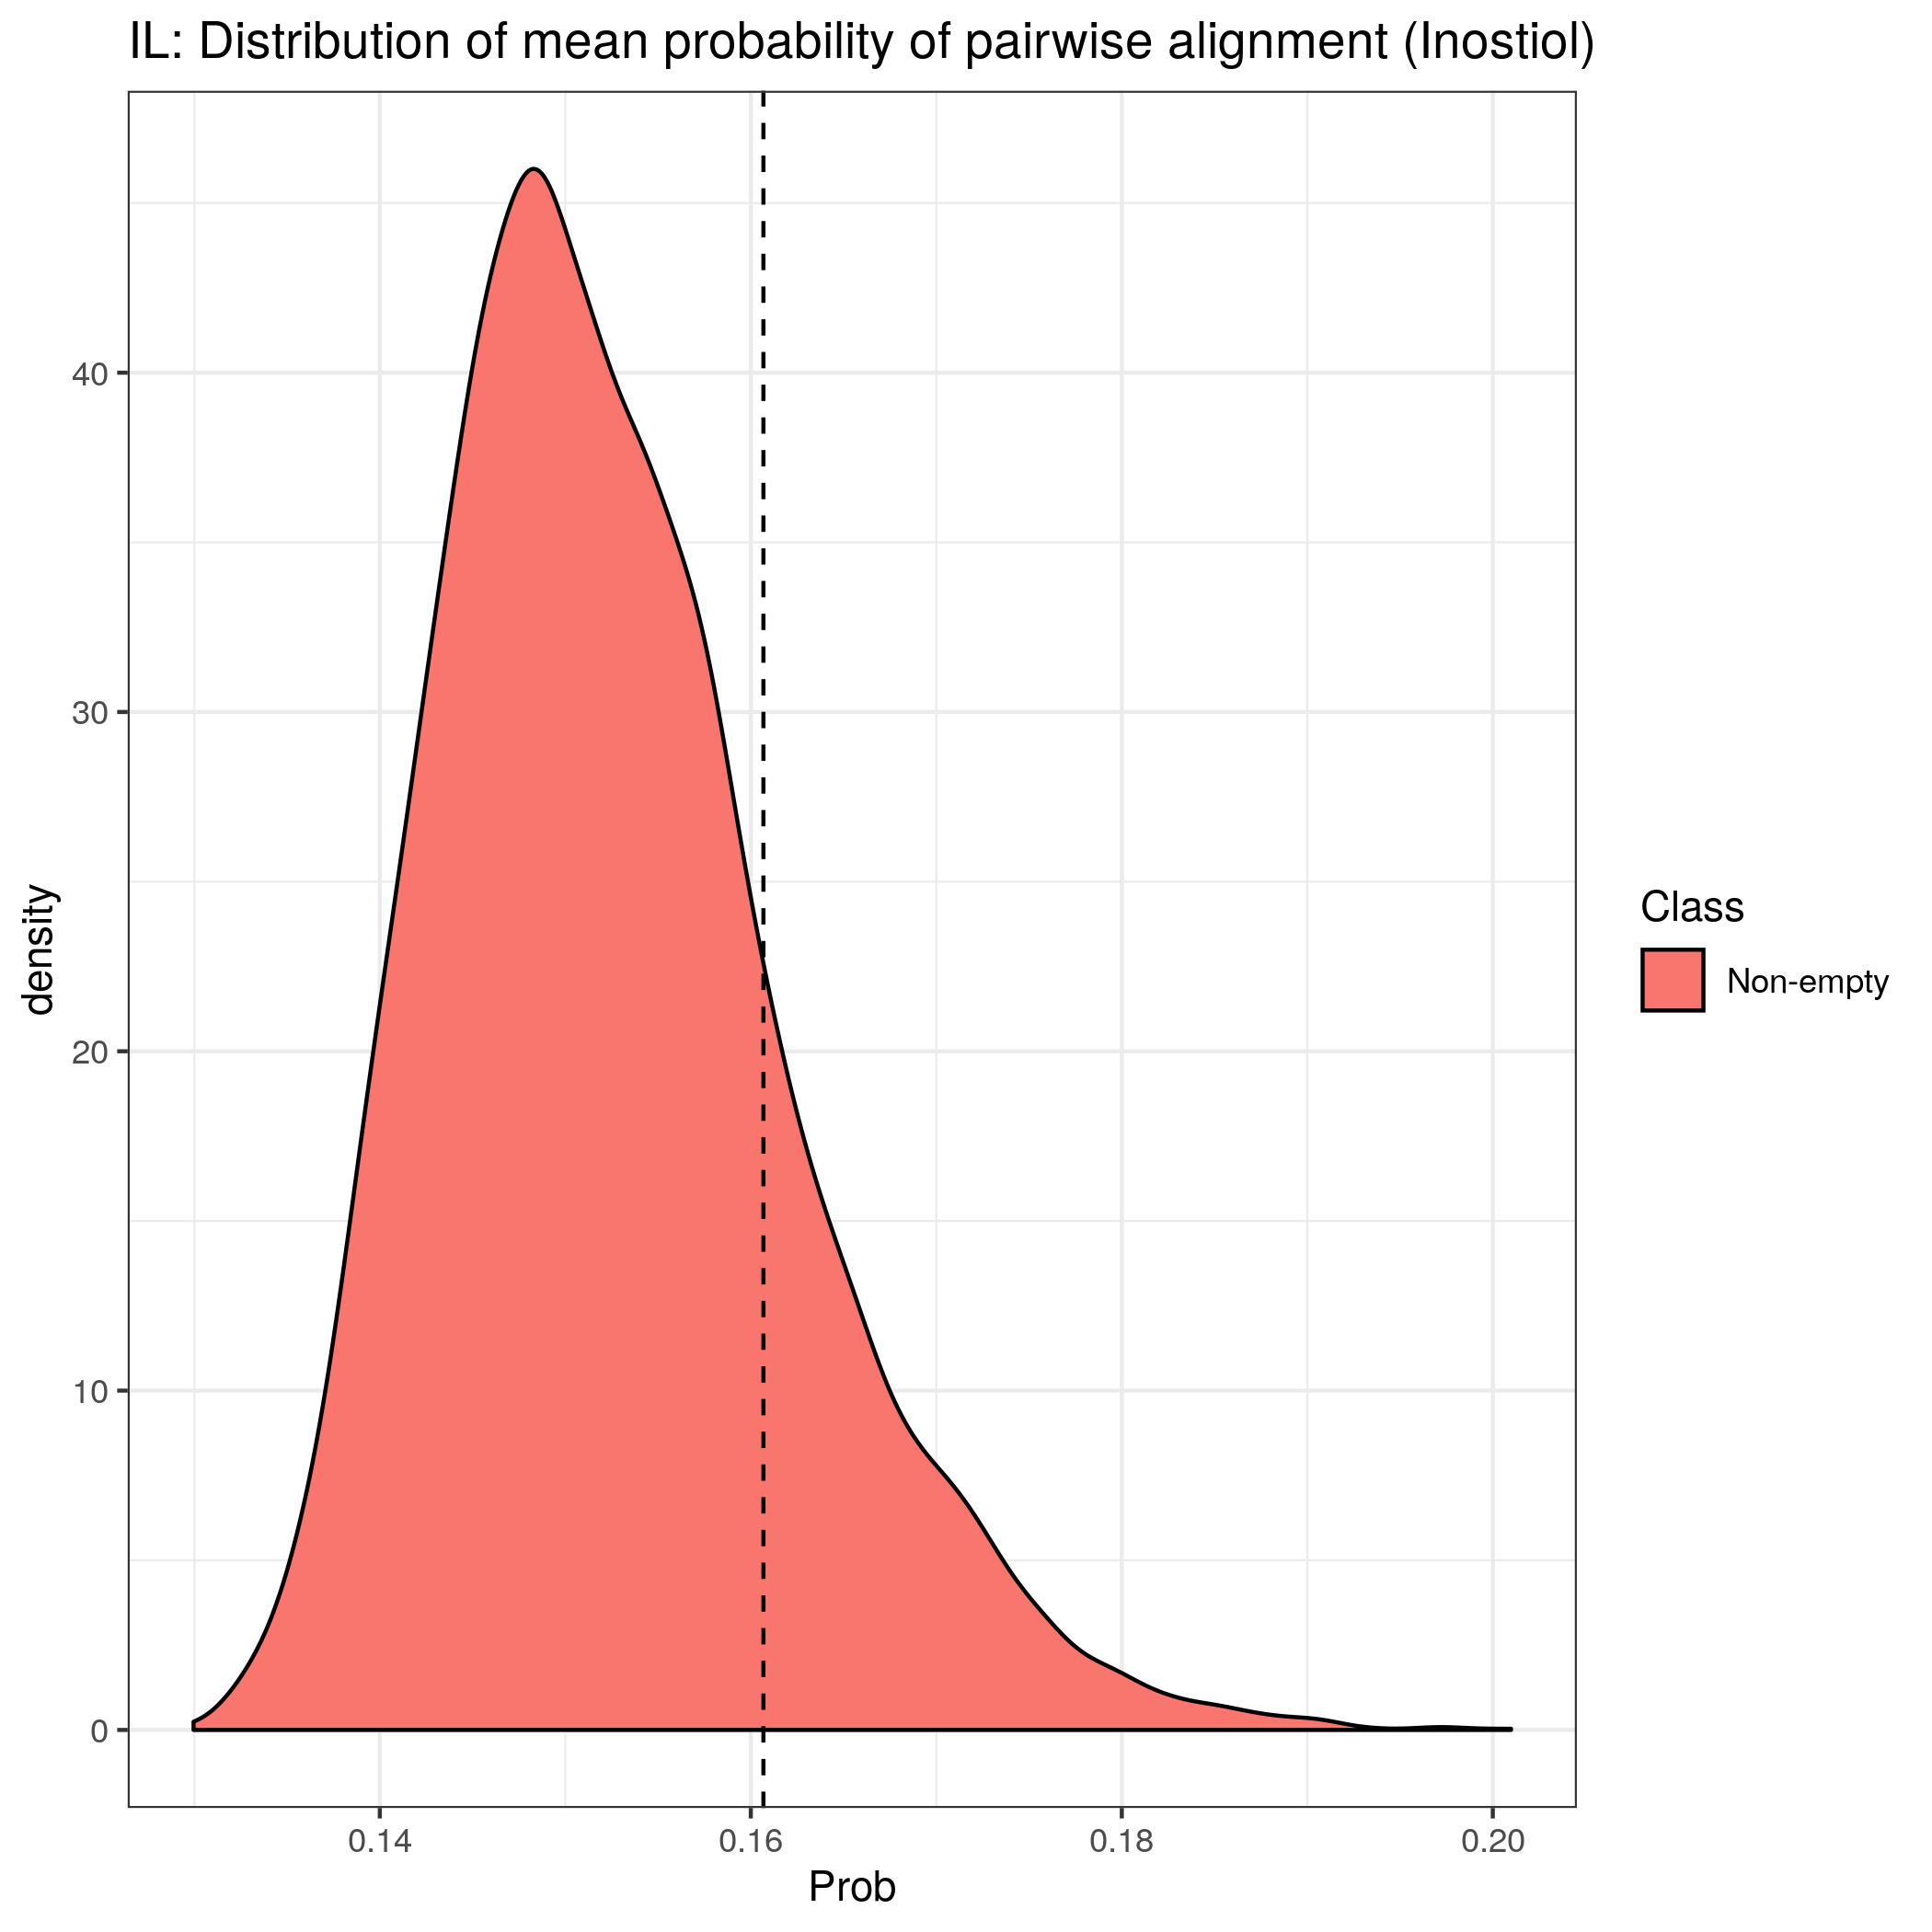
\includegraphics[scale=0.75]{Images/Biology_data/Set_250/All_datasets/Mean_alignment_probability/IL_KEGG_INOSITOL_PHOSPHATE_METABOLISM.png}
		\caption{CEDAR Case 1: Plot of the distribution of the mean probability of pairwise alignment for a random sample of 60 genes with a dashed line indicating the mean probability of pairwise alignment for the Inositol genes in the IL dataset for the 250 probe set.}
		\label{fig:results:cedar_1:mdi_il_inostiol_alignemnt_prob_distn}
	\end{figure}


\begin{figure}[h]
	\centering
	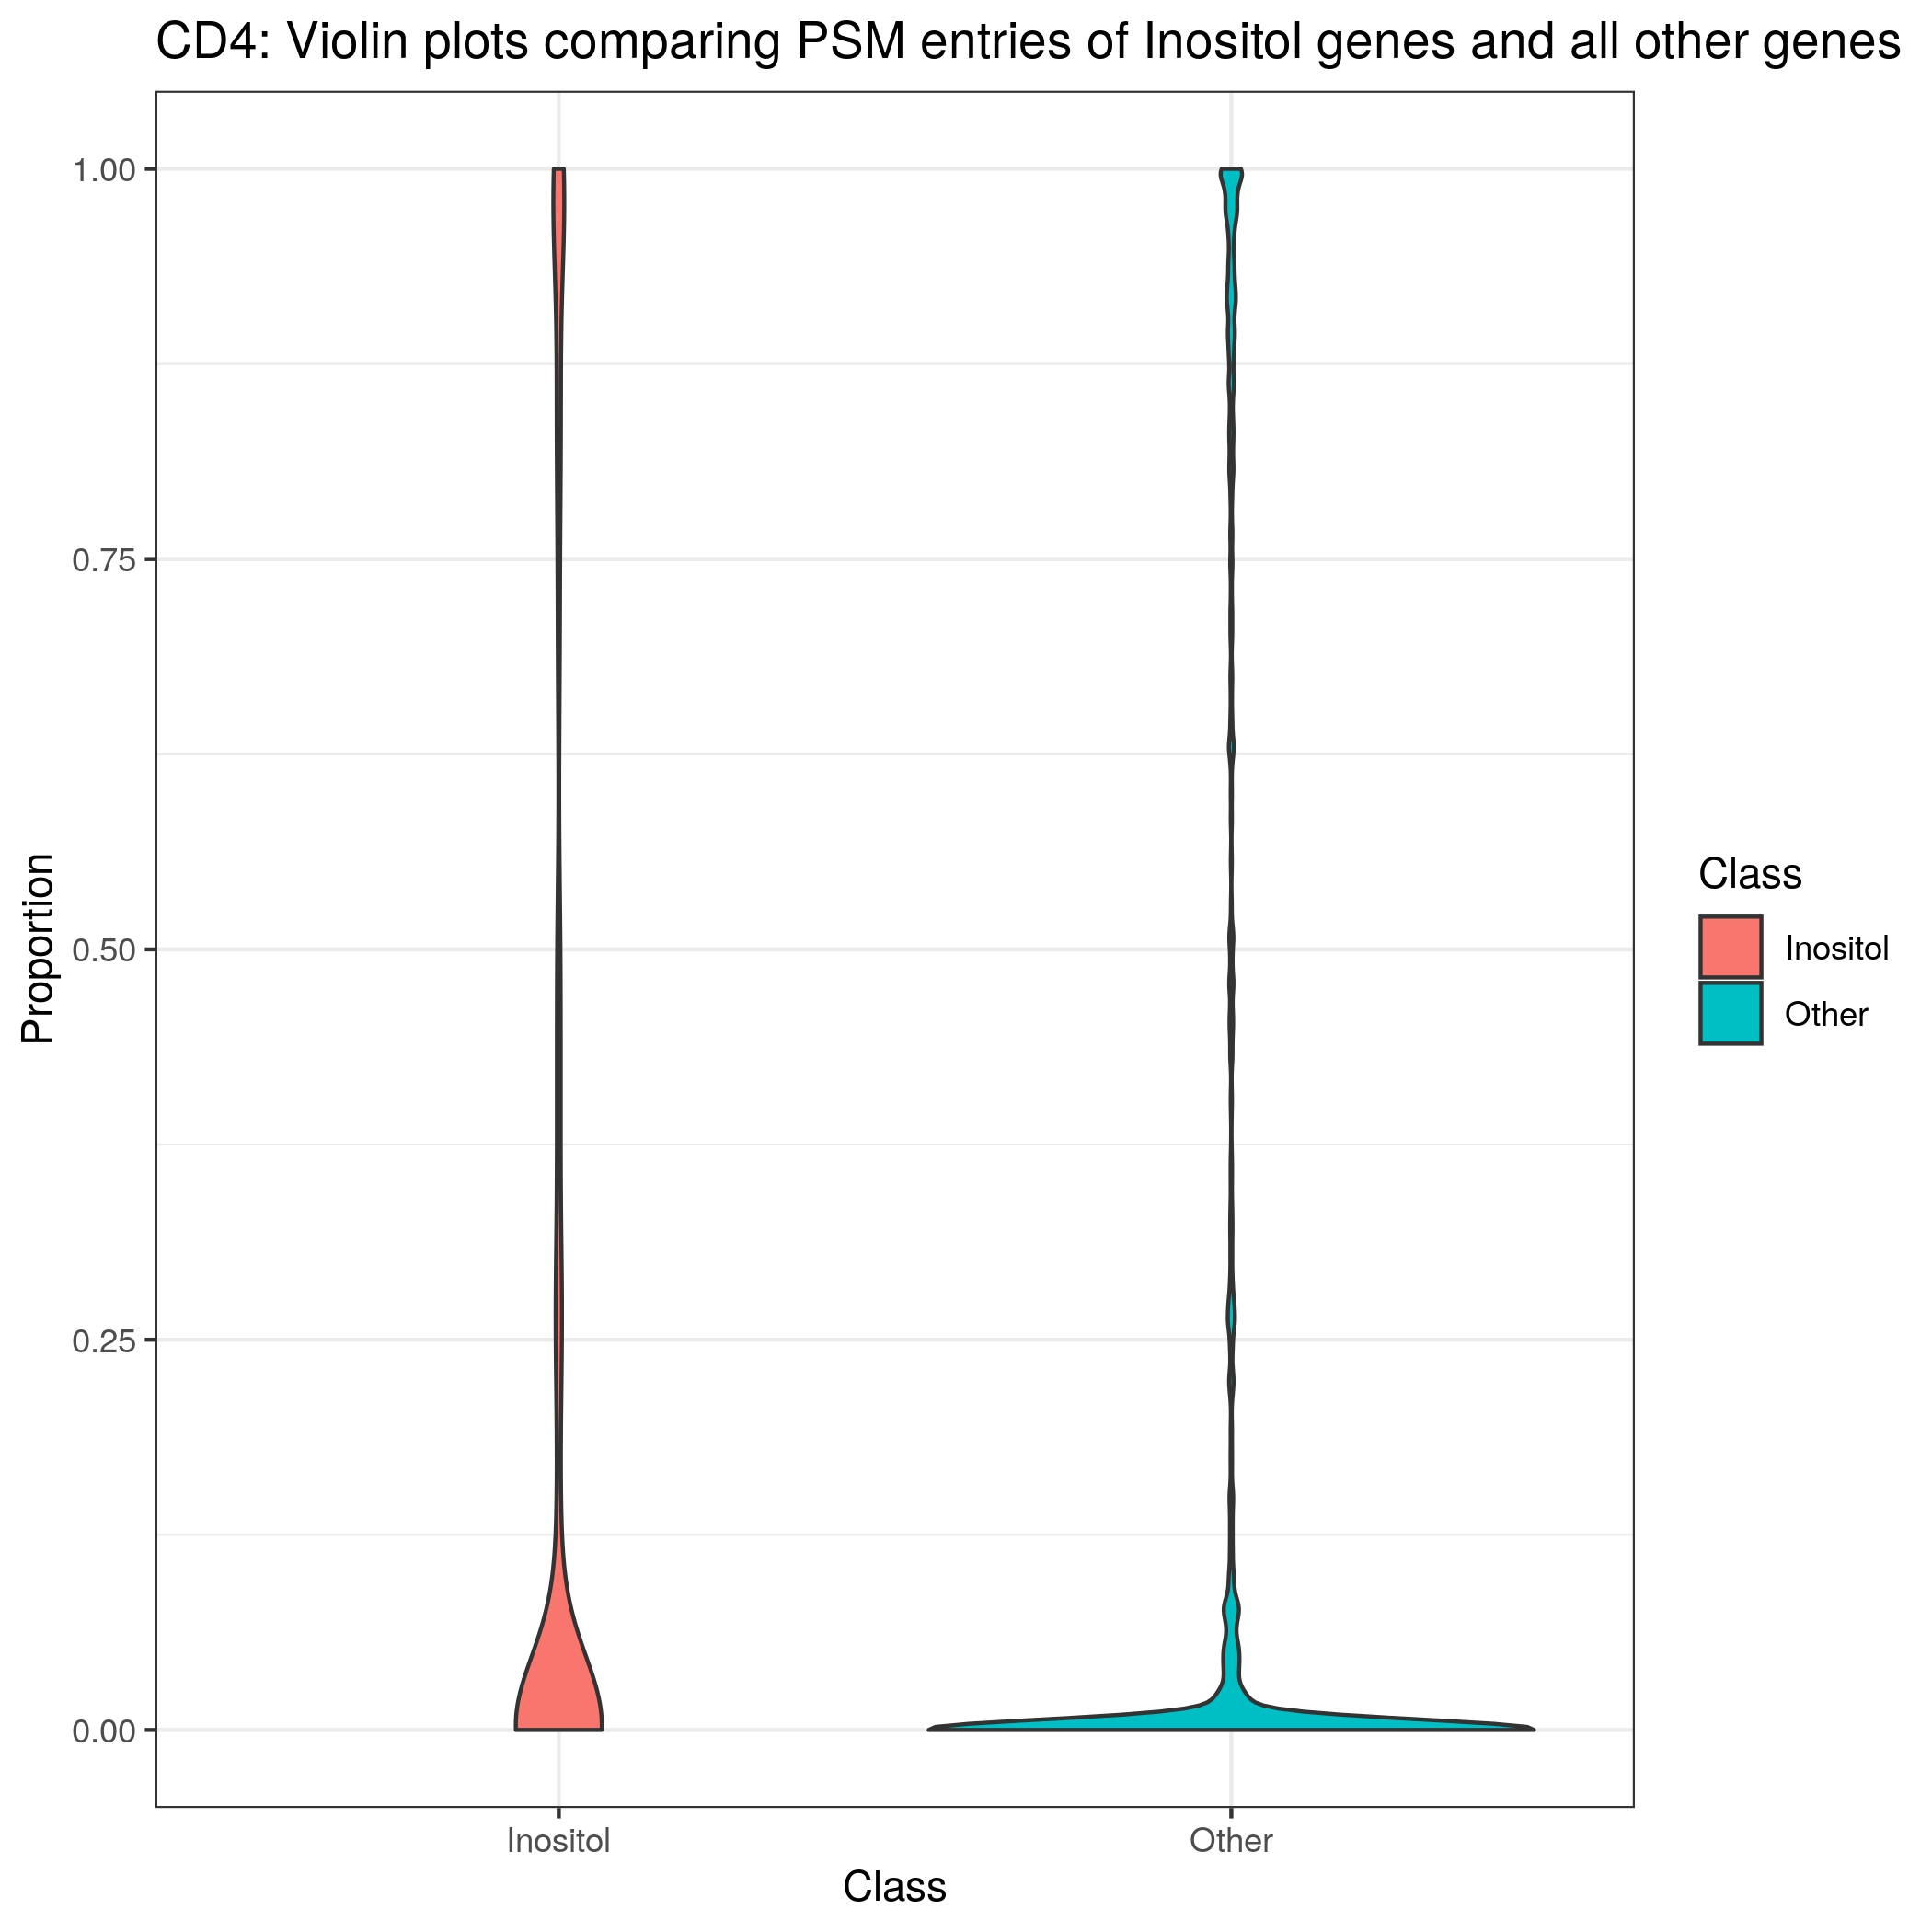
\includegraphics[scale=0.75]{Images/Biology_data/Set_250/All_datasets/PSM_densities/KEGG_INOSITOL_PHOSPHATE_METABOLISM/CD4.png}
	\caption{CEDAR Case 1: Violin plot of the PSM entries for the Inositol genes and the genes not belonging to this pathway for the CD4 datasets from the consensus clustering of MDI.}
	\label{fig:results:cedar_1:mdi_cd4_inostiol_psm_violin}
\end{figure}
%	\newpage
	
	I include a direct comparison of the PSM from MDI to the single dataset case in figure \ref{fig:results:cedar_1:mdi_mixture_model_comp_tr}. It can be seen that there is similarity in the structure uncovered, but thanks to sharing of common information MDI appears to be more confident in its allocation. There are less blocks in the first PSM (or rather within each block there is more confidence, whereas the mixture model is less certain of the homogeneity of membership within any cluster).
	
%	\newpage
	
	\begin{sidewaysfigure} %[h]
		\centering
		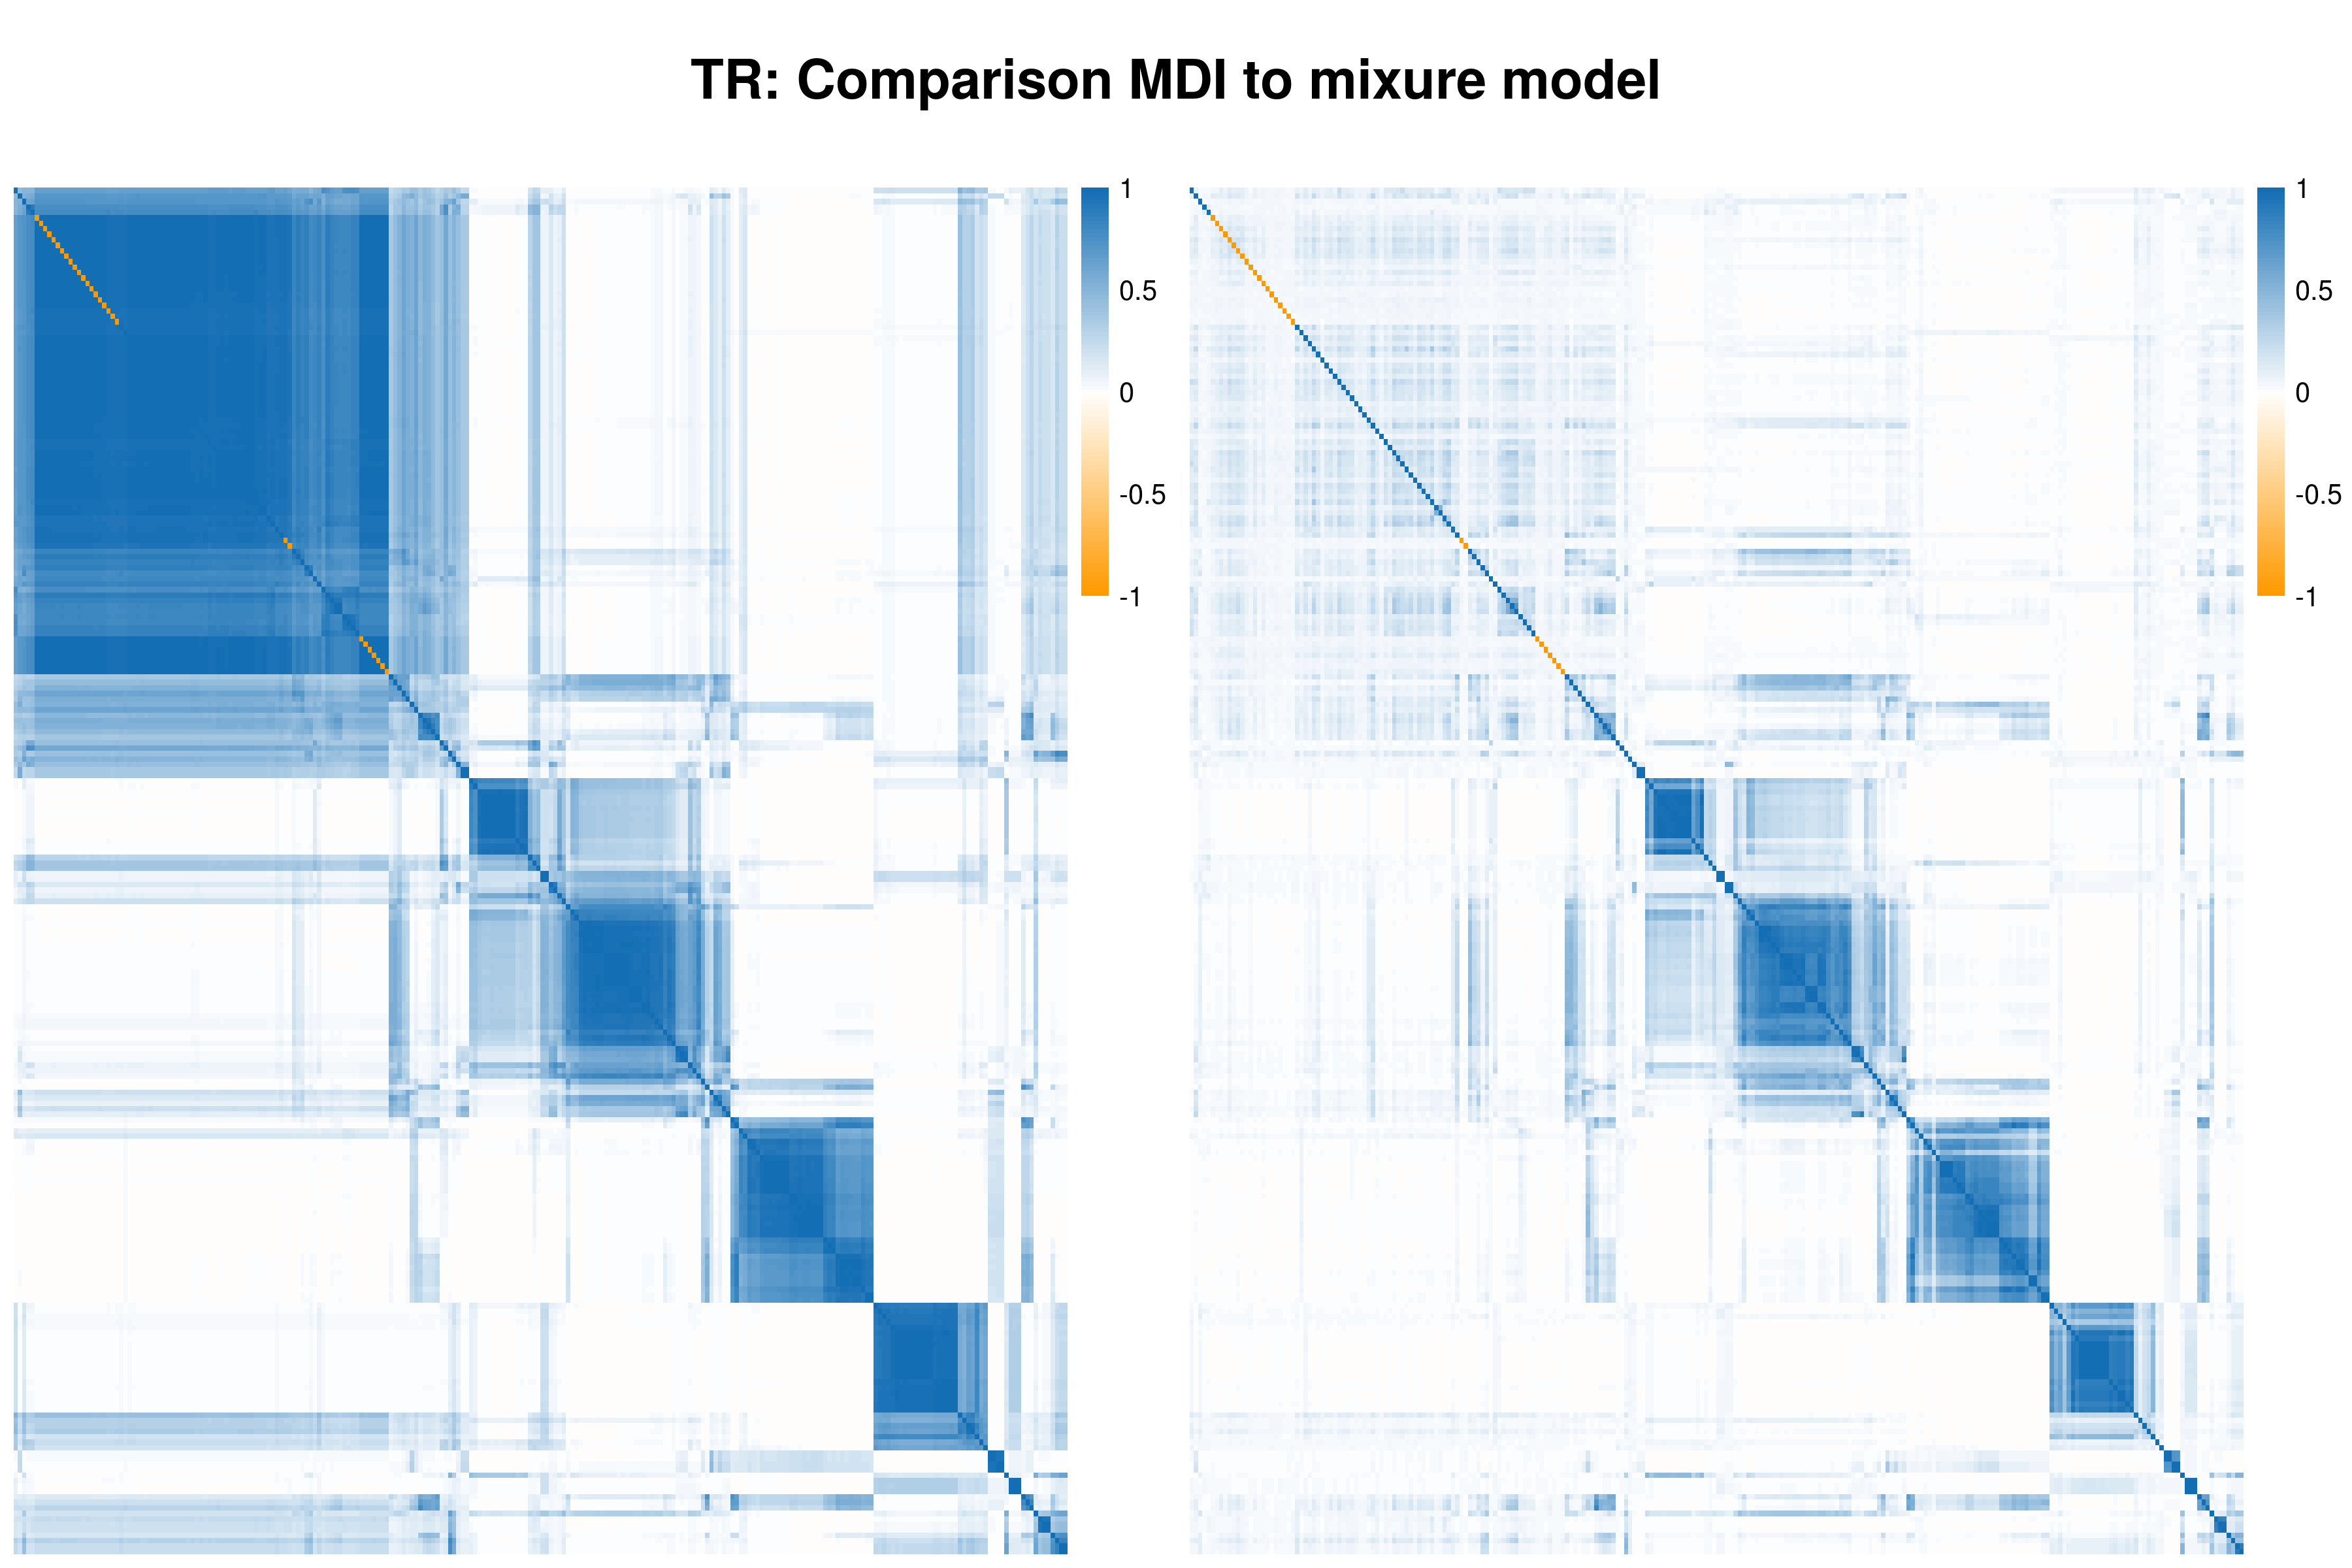
\includegraphics[scale=0.75]{Images/Biology_data/Set_250/Comparison_mdi_mixture_model/TR_comparison_all_specific_sim.png}
		\caption{CEDAR Case 1: Comparison of the PSMs generated by applying consensus clustering using an MDI model and individual mixture models using only the TR dataset. Thanks to sharing of common information MDI appears to be more confident in its allocation. There are less blocks in the first PSM (or rather within each block there is more confidence, whereas the mixture model is less certain of the homogeneity of membership within any cluster).}
		\label{fig:results:cedar_1:mdi_mixture_model_comp_tr}
	\end{sidewaysfigure}
	
	A comparison between a Bayesian mixture model and consensus clustering inference of mixture models is also performed. Three chains of 1 million iterations with a thinning factor of 50 were generated. One can see in a comparison of the three PSMs for CD14 (figure \ref{fig:results:cedar_1:cd14_bayes_mixture_model_comp}) that there is no uncertainty in the individual PSMs, but that each has achieved a different mode. A comparison of the PSM from one of these chains with the correlation matrix and the standardised data can be seen in figure \ref{fig:results:cedar_1:cd14_bayes_mixture_model_comp_seed_1}. Here, one can see that the results are representative of some of the correlation structure, but that the model does capture any uncertainty. This shows that even if MDI was computationally feasible to run on this dataset it would not converge in a reasonable time.
	
	\begin{sidewaysfigure} %[h]
		\centering
		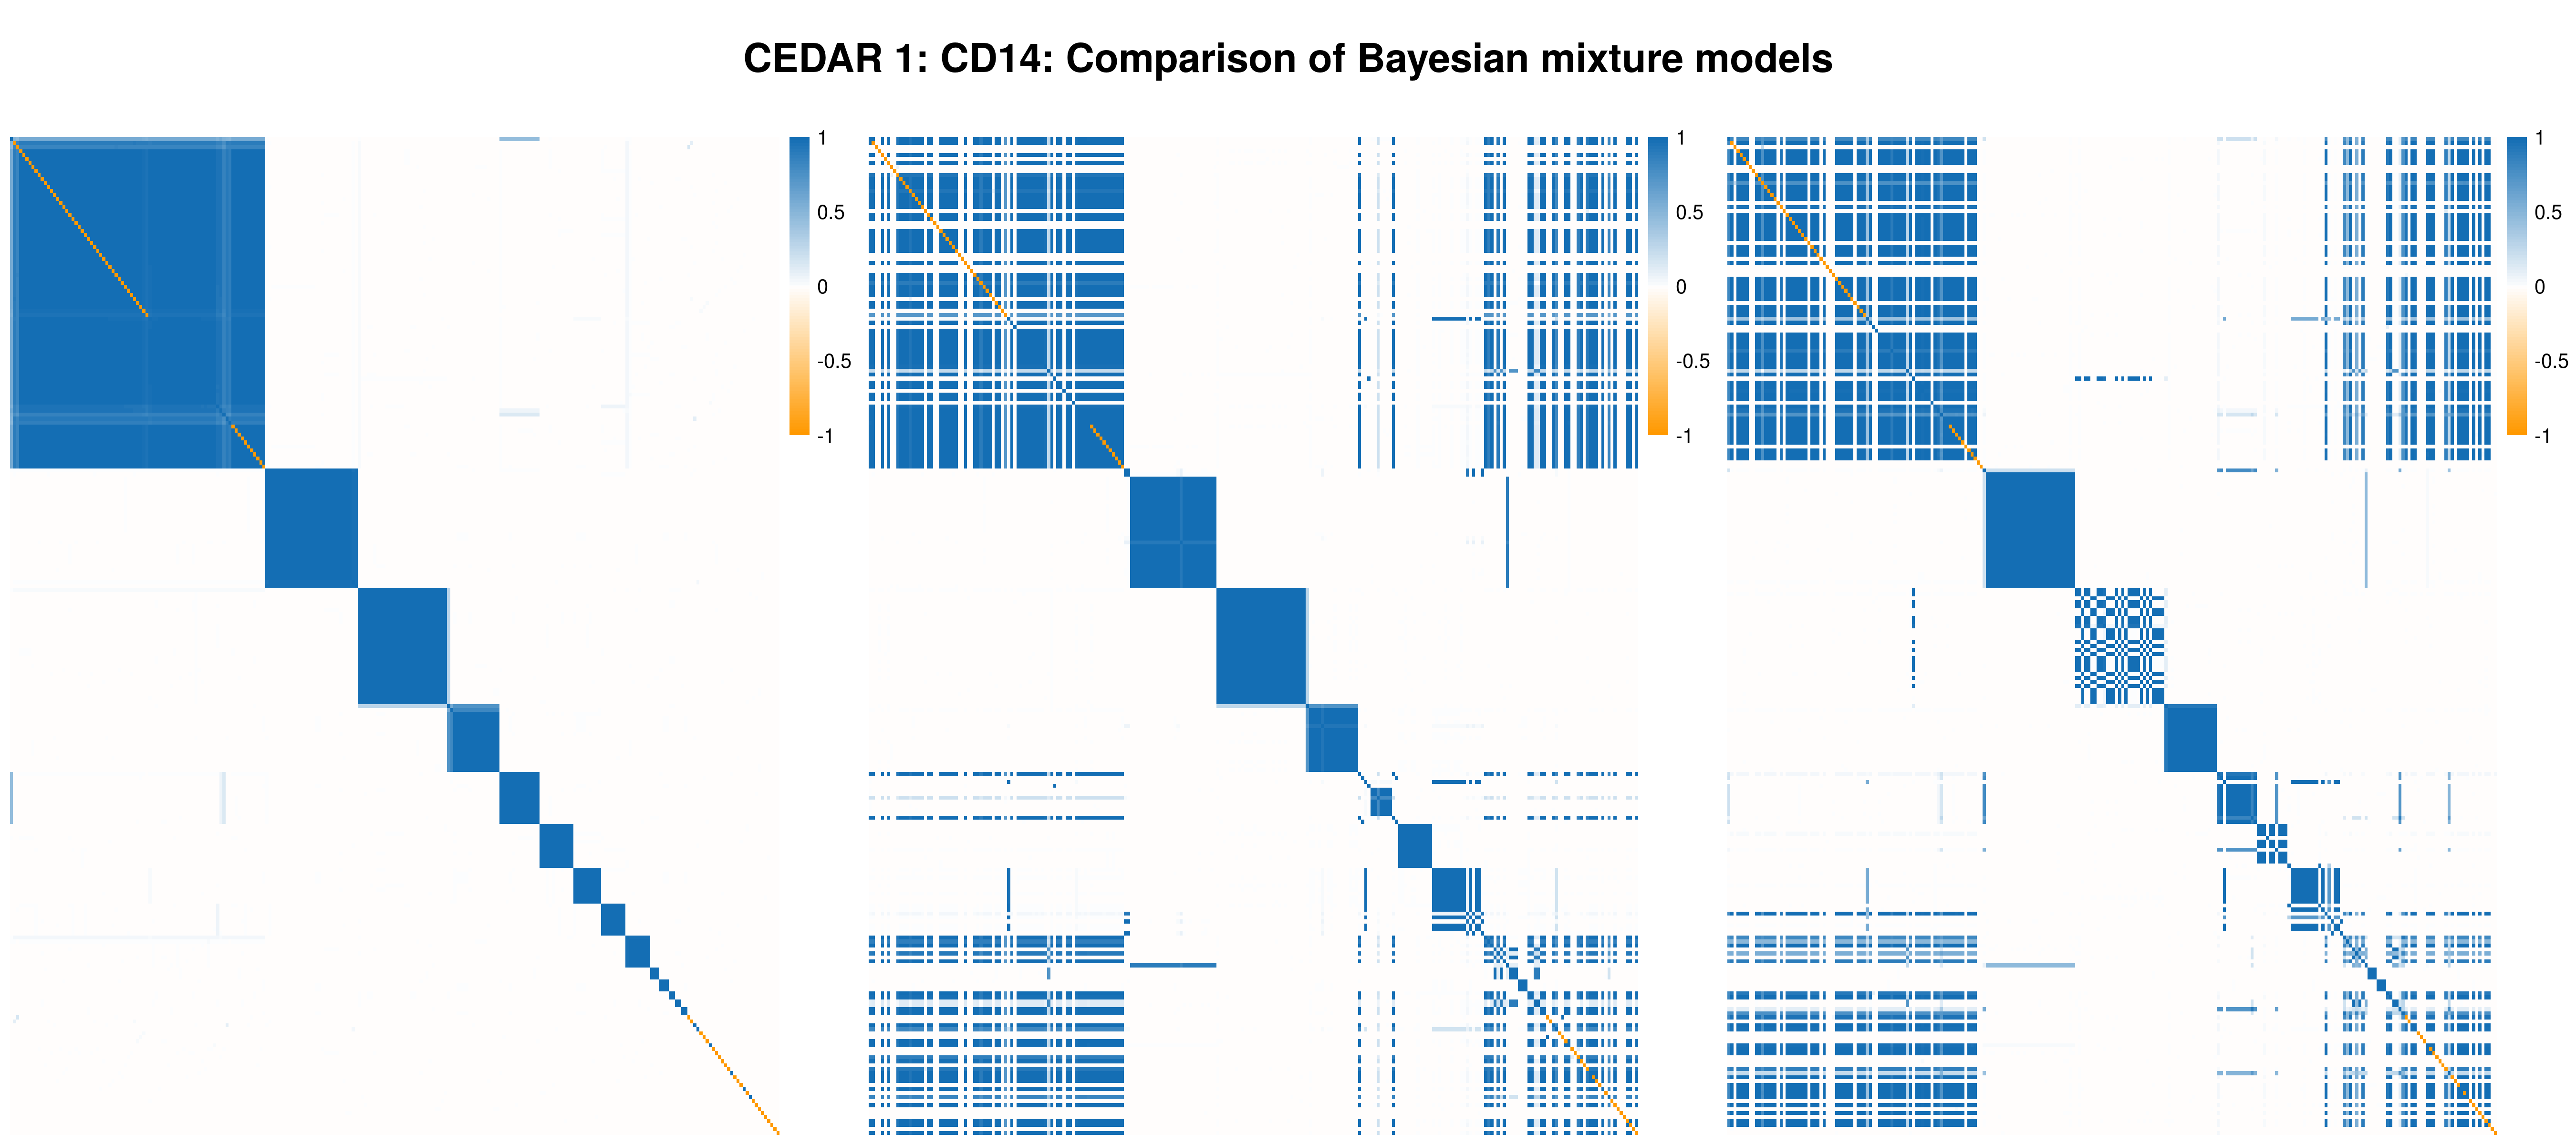
\includegraphics[scale=0.5]{Images/Biology_data/Set_250/Bayesian_mixture_models/CD14_comparison_across_seeds.png}
		\caption{CEDAR Case 1: Comparison of the PSMs generated by for three different chains of a Bayesian mixture model for the CD14 data in the set of 250 probes (ordered by the first PSM). One can see that the three PSMs agree on two clusters completely but otherwise achieve different modes.}
		\label{fig:results:cedar_1:cd14_bayes_mixture_model_comp}
	\end{sidewaysfigure}

	\begin{sidewaysfigure} %[h]
		\centering
		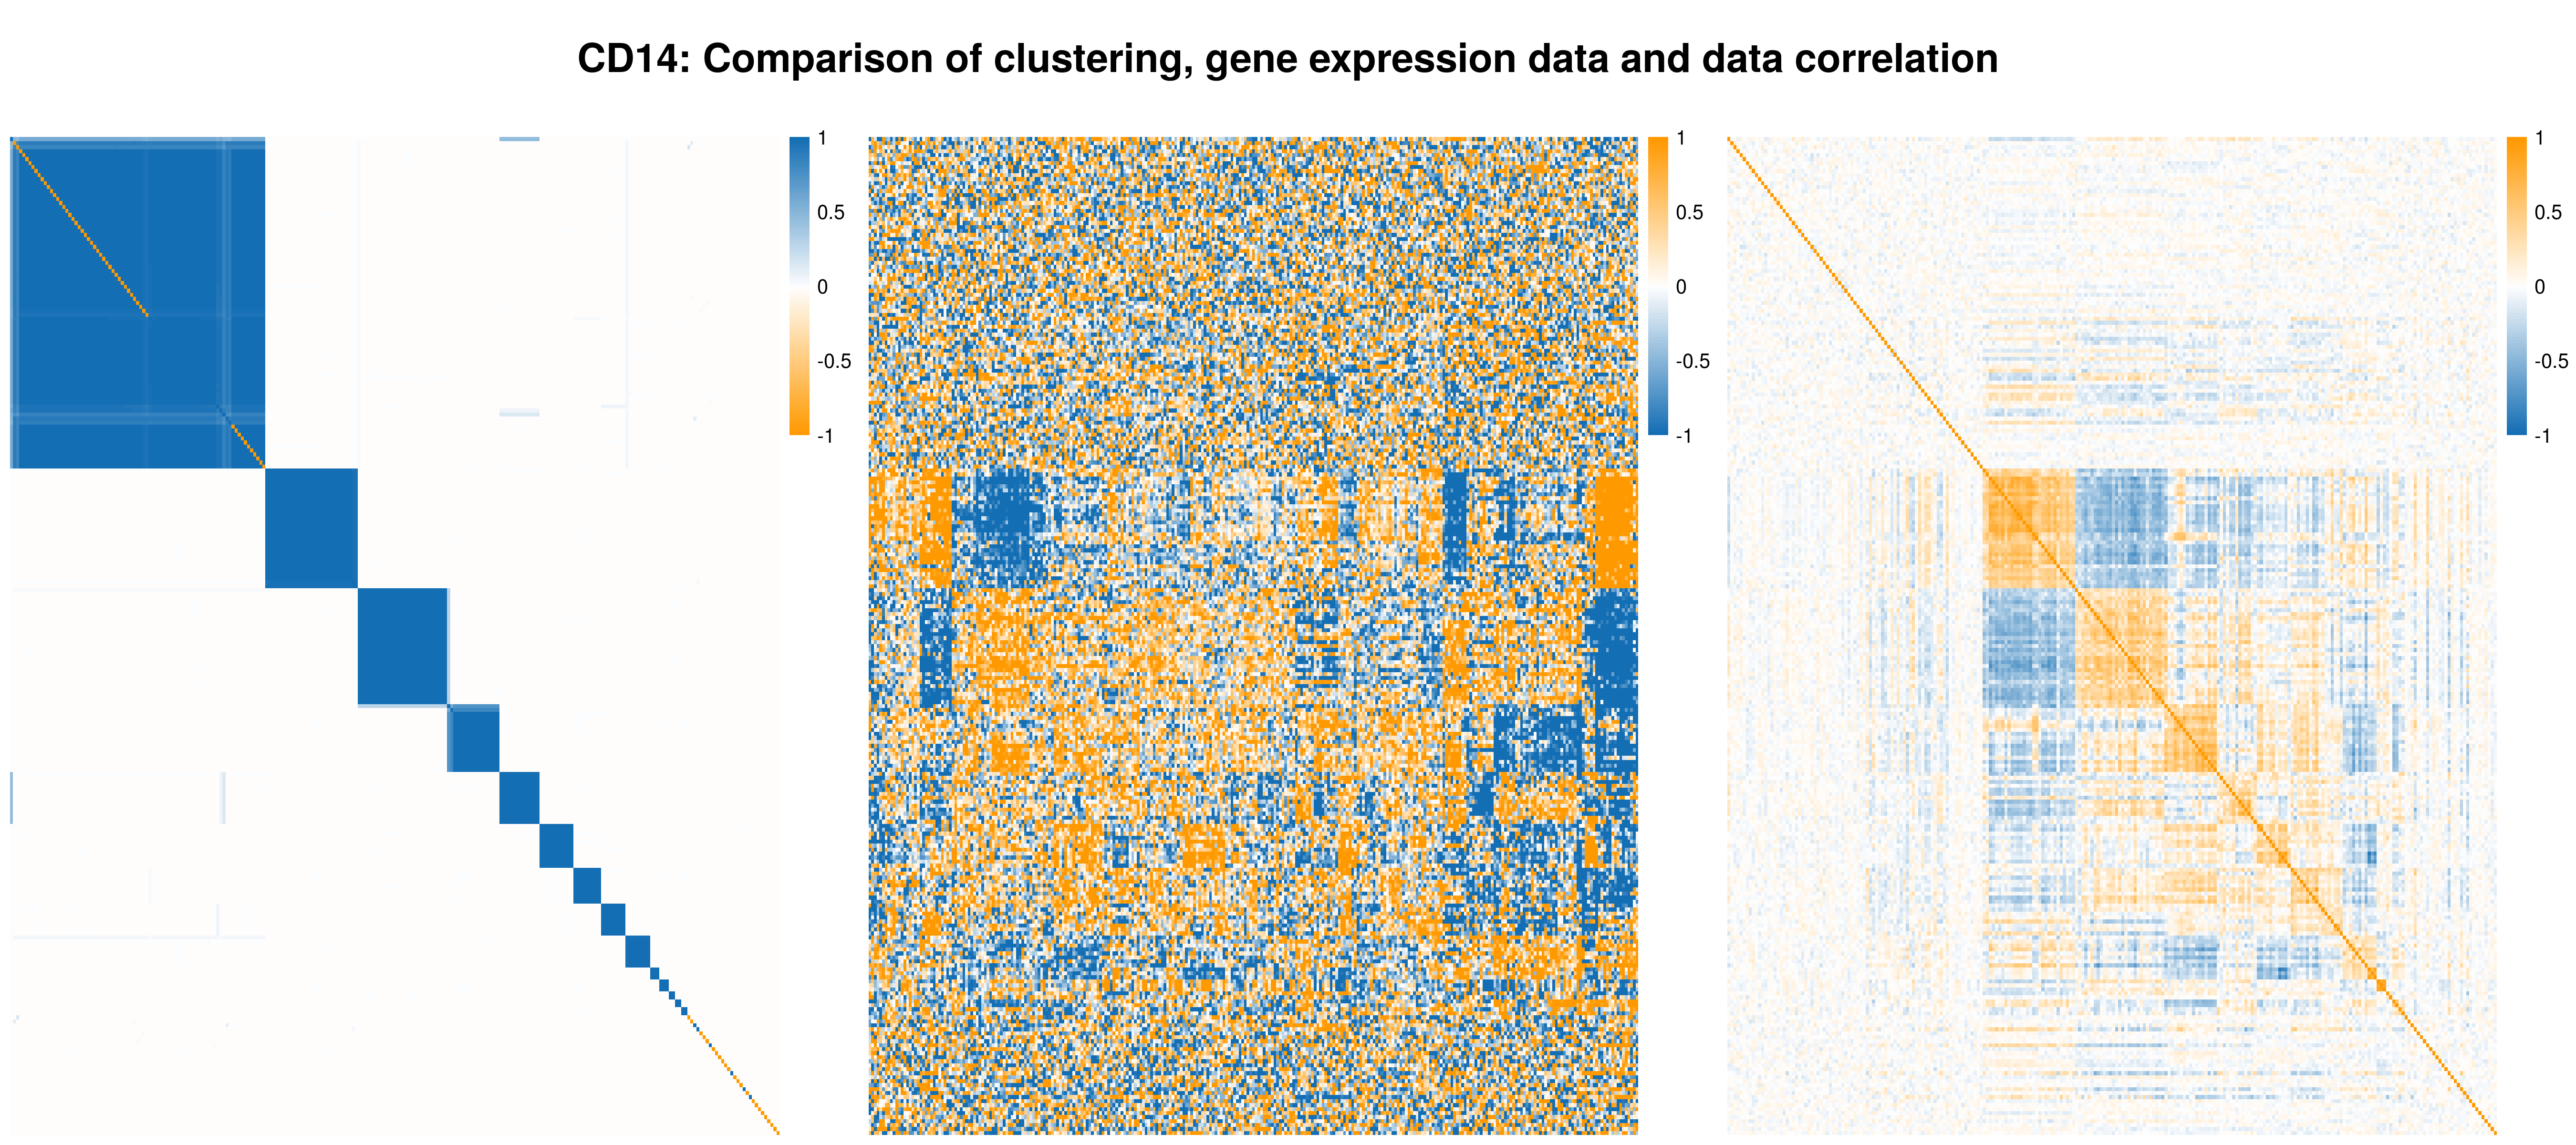
\includegraphics[scale=0.45]{Images/Biology_data/Set_250/Bayesian_mixture_models/Comparison_expression_clustering_correlation/CD14.png}
		\caption{CEDAR Case 1: Comparison of the PSM for the Bayesian mixture model for CD14 with a seed of 1 (corresponding to the PSM on the left in figure \ref{fig:results:cedar_1:cd14_bayes_mixture_model_comp}) with the standardised expression data and its correlation matrix. One can see that the results are representative of some of the correlation structure, but that the model does capture any uncertainty. This shows why even if MDI was computationally feasible to run on this dataset it would not converge in a reasonable time.}
		\label{fig:results:cedar_1:cd14_bayes_mixture_model_comp_seed_1}
	\end{sidewaysfigure}
	
%	\newpage
	
%	If a pathway has $m$ members present in a dataset, we sampled $m$ random genes not in this pathway and found the mean probability of the pairwise alignment of these genes (i.e. the proportion of seeds for which any two of the $m$ genes had the same labelling). Taking $n$ of these samples allowed us to describe the distribution of the mean pairwise alignment probability and compare with the mean pairwise alignment probability of the $m$ genes from the pathway of interest.
%	
%	The violin plots of the PSM entries for each pathway were compared to the PSM entries for the remaining genes in the dataset.
	
	\subsubsection{Case 2: 1,000 probes} \label{sec:results:cedar:dataset_2}
	Each chain of 500 iterations took approximately 12 hours and 0 minutes to run. Results for the pipeline described in the list \ref{list:cedar_pipeline_analysis}, i.e. the results before KEGG pathway analysis, can be seen in figures \ref{fig:results:cedar_2:mdi_cd4_adj_rand_ind_plot}, \ref{fig:results:cedar_2:mdi_adj_rand_ind_heatmap}, \ref{fig:results:cedar_2:mdi_re_tr_phi_series_plot}, \ref{fig:results:cedar_2:mdi_re_tr_phi_histogram}, \ref{fig:results:cedar_2:mdi_phi_heatmap}, \ref{fig:results:cedar_2:mdi_cd4_number_clusters_plot},  \ref{fig:results:cedar_2:mdi_cd4_mass_parameter_plot}, \ref{fig:results:cedar_2:mdi_cd4_psm} and  \ref{fig:results:cedar_2:mdi_cd4_psm_expr_cor}. These results are in keeping with those from section \ref{sec:results:cedar:dataset_1}; there has not been a shift in results now that a larger subset of the CEDAR data is being used. In short, the consensus clustering is exploring a variety of clusterings across seeds (figures \ref{fig:results:cedar_2:mdi_cd4_adj_rand_ind_plot}, \ref{fig:results:cedar_2:mdi_re_tr_phi_series_plot} and \ref{fig:results:cedar_2:mdi_re_tr_phi_histogram}) and the PSM does align with the correlation matrix and standardised data (figure \ref{fig:results:cedar_2:mdi_cd4_psm_expr_cor}), capturing uncertainty of cluster membership (figure \ref{fig:results:cedar_2:mdi_cd4_psm}). The CD datasets have similar clustering structure as do the intestinal samples with little information shared across these groups. Within this data comparison, the T lymphocyte datasets, CD4 and CD8 are particularly similar (figures \ref{fig:results:cedar_2:mdi_cd4_adj_rand_ind_plot} and \ref{fig:results:cedar_2:mdi_cd4_adj_rand_ind_plot}).
	
%	\begin{enumerate}
%		\item The adjusted Rand index between $i^{th}$ and $1,000^{th}$ clusterings were plotted for all $i\in \{1,\ldots,1000\}$ (see an example in figure \ref{fig:results:cedar_2:mdi_cd4_adj_rand_ind_plot});
%		\item The mean adjusted Rand index comparing clusterings across datasets were represented in a heatmap (see figure \ref{fig:results:cedar_2:mdi_adj_rand_ind_heatmap});
%		\item The $\phi_{ij}$ values were plotted across seeds for all combinations of datasets (see an example in  figure \ref{fig:results:cedar_2:mdi_re_tr_phi_series_plot});
%		\item The distribution of $\phi_{ij}$ values were plotted for all combinations of datasets (see an example in  figure \ref{fig:results:cedar_2:mdi_re_tr_phi_histogram});
%		\item The mean $\phi$ value between datasets are represented in a heatmap (see figure \ref{fig:results:cedar_2:mdi_phi_heatmap});
%		\item The number of clusters present in any given seed were plotted for each dataset (see an example in  figure \ref{fig:results:cedar_2:mdi_cd4_number_clusters_plot});
%		\item The mass parameter for the underlying mixture models were plotted across seeds for each dataset (see an example in  figure \ref{fig:results:cedar_2:mdi_cd4_mass_parameter_plot});
%		\item The PSM for each dataset was plotted as a heatmap (see an example in  figure \ref{fig:results:cedar_2:mdi_cd4_psm}); and
%		\item The comparison of the PSM, the standardised expression data and the correlation matrix were plotted with a common row ordering for each dataset (see an example in  figure \ref{fig:results:cedar_2:mdi_cd4_psm_expr_cor}). %; and
%		%		\item The expression of fused genes was plotted for all dataset combinations (see an example in  figure \ref{fig:mdi_cd4_cd8_fused_genes}).
%	\end{enumerate}
	
%	\newpage
	
	\begin{figure}[h]
		\centering
		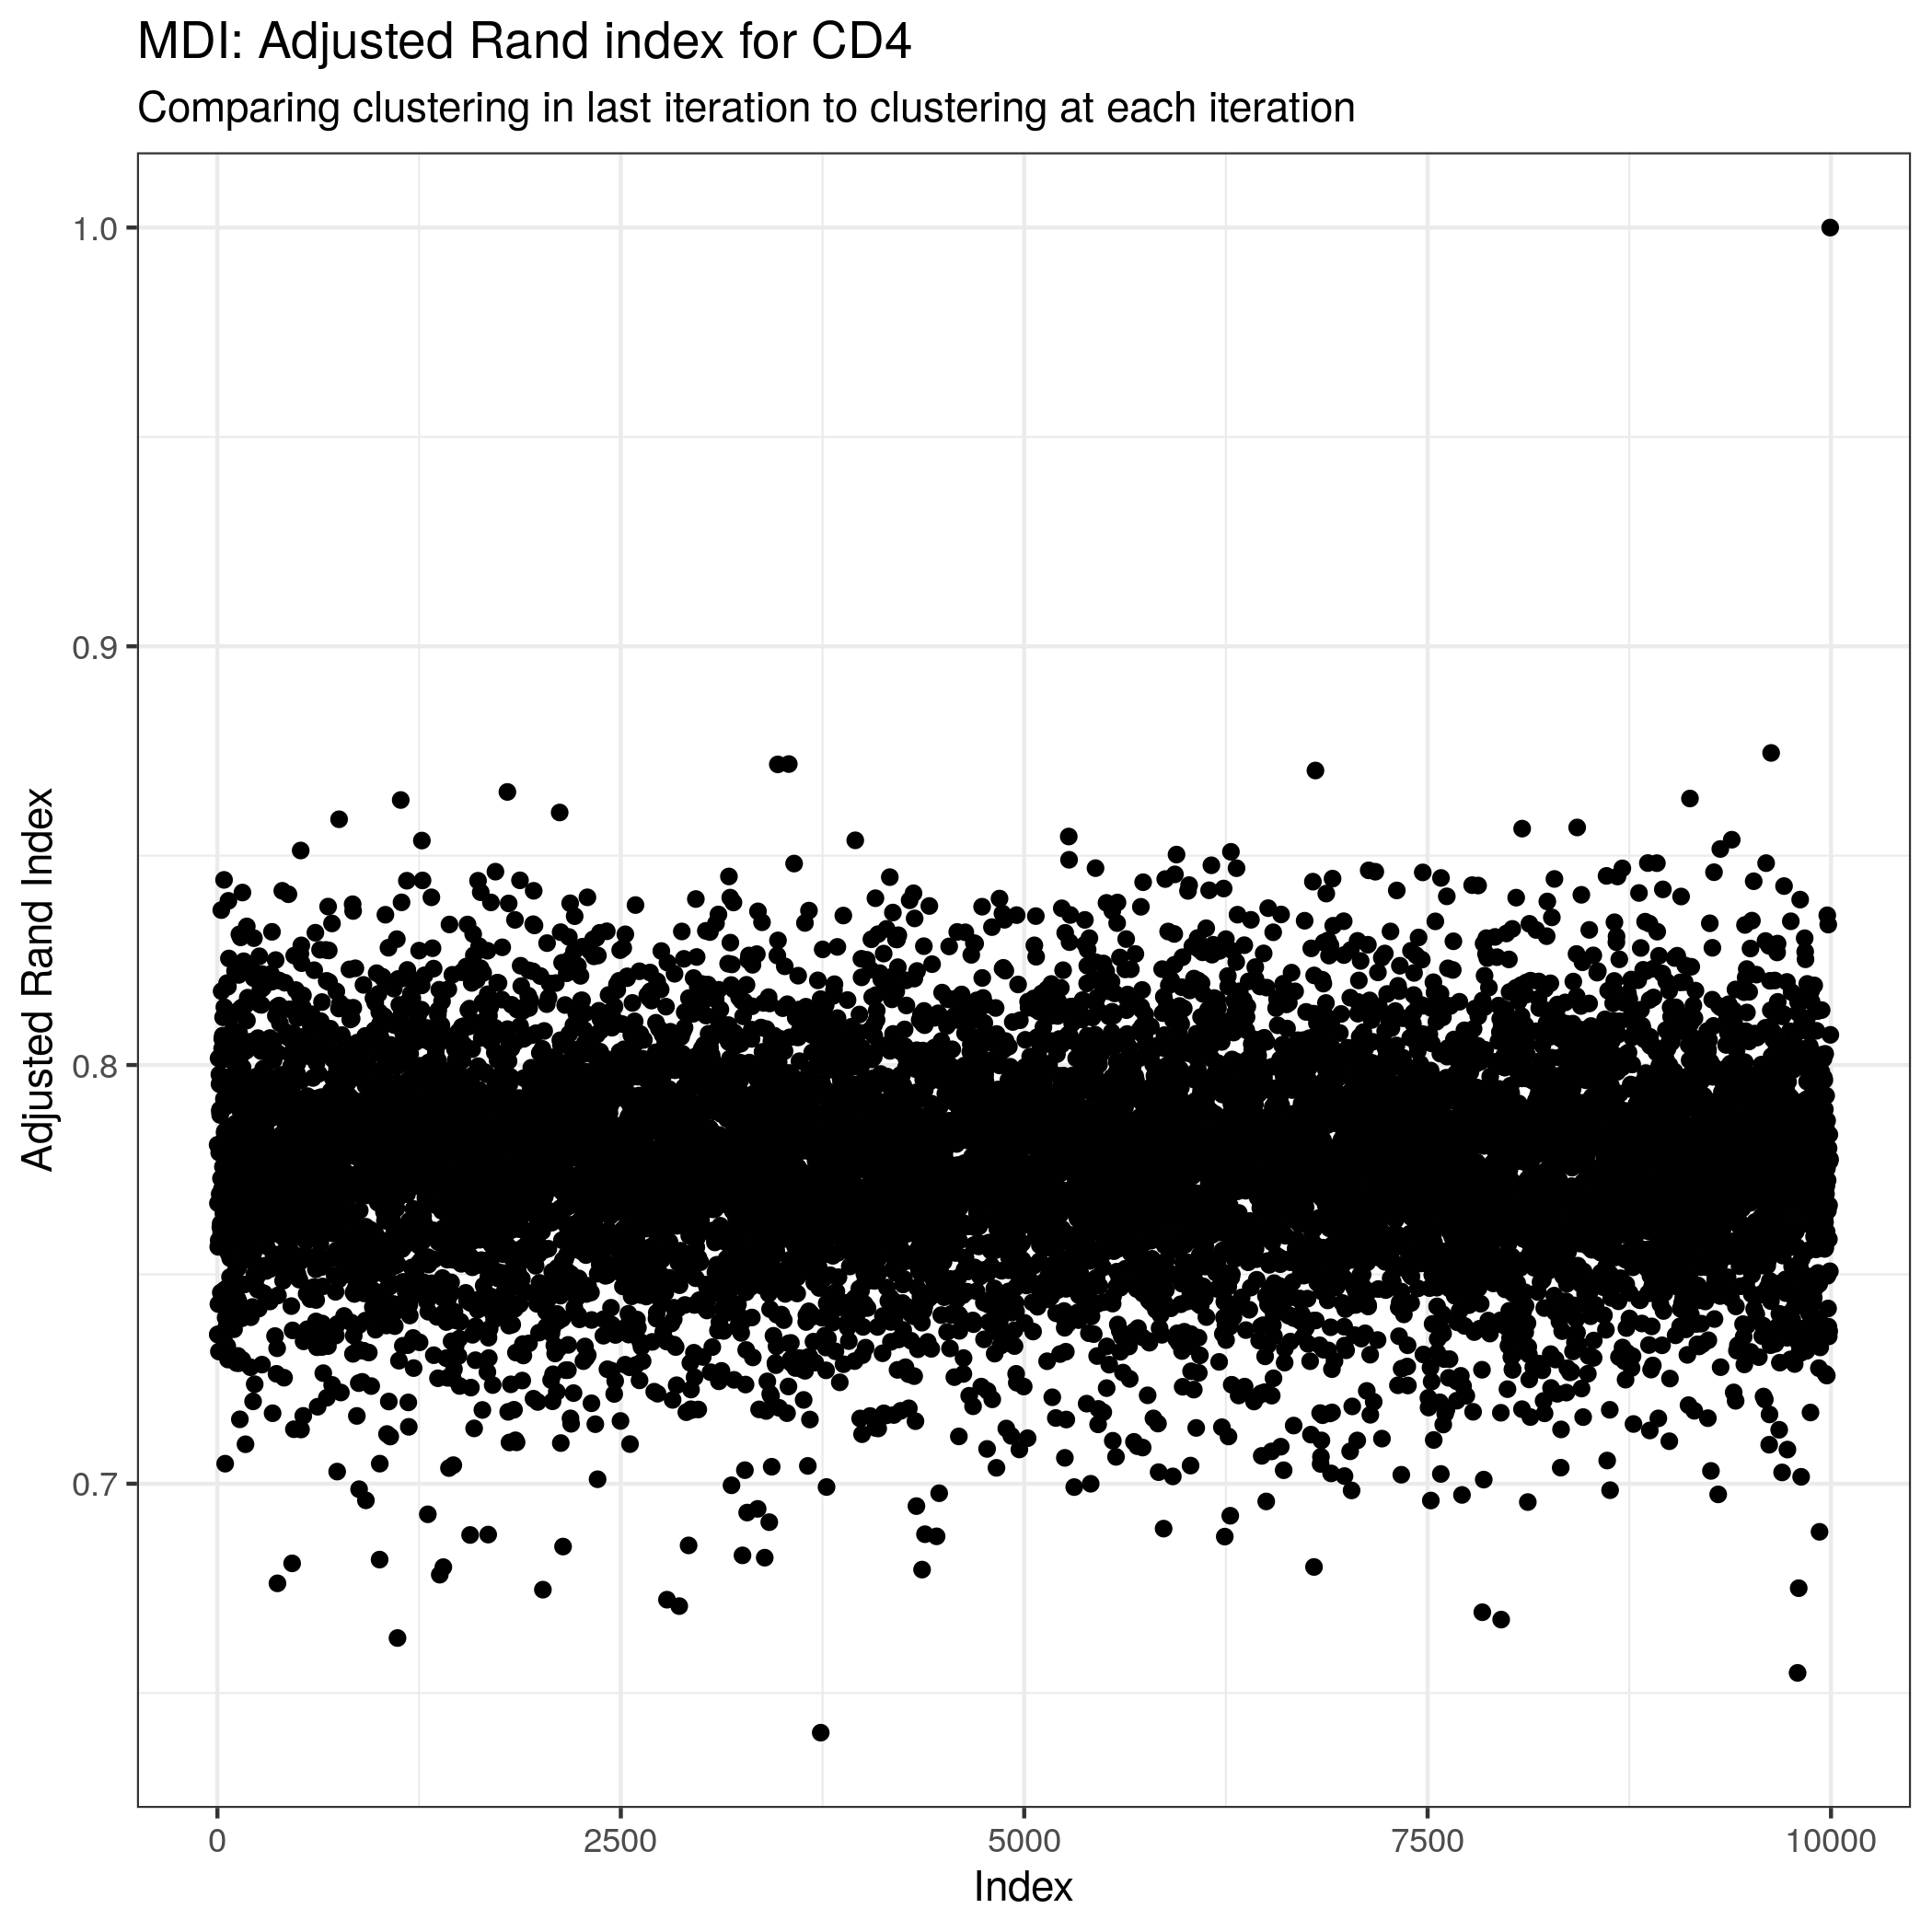
\includegraphics[scale=0.75]{Images/Biology_data/Set_1000/All_datasets/Adjusted_rand_index_plots/rand_index_plot_CD4.png}
		\caption{CEDAR Case 2: Plot of the adjusted Rand index between the clustering in each seed to that in the 1,000$^{th}$ for CD14.}
		\label{fig:results:cedar_2:mdi_cd4_adj_rand_ind_plot}
	\end{figure}
	
%	\newpage
	
	\begin{figure}[h]
		\centering
		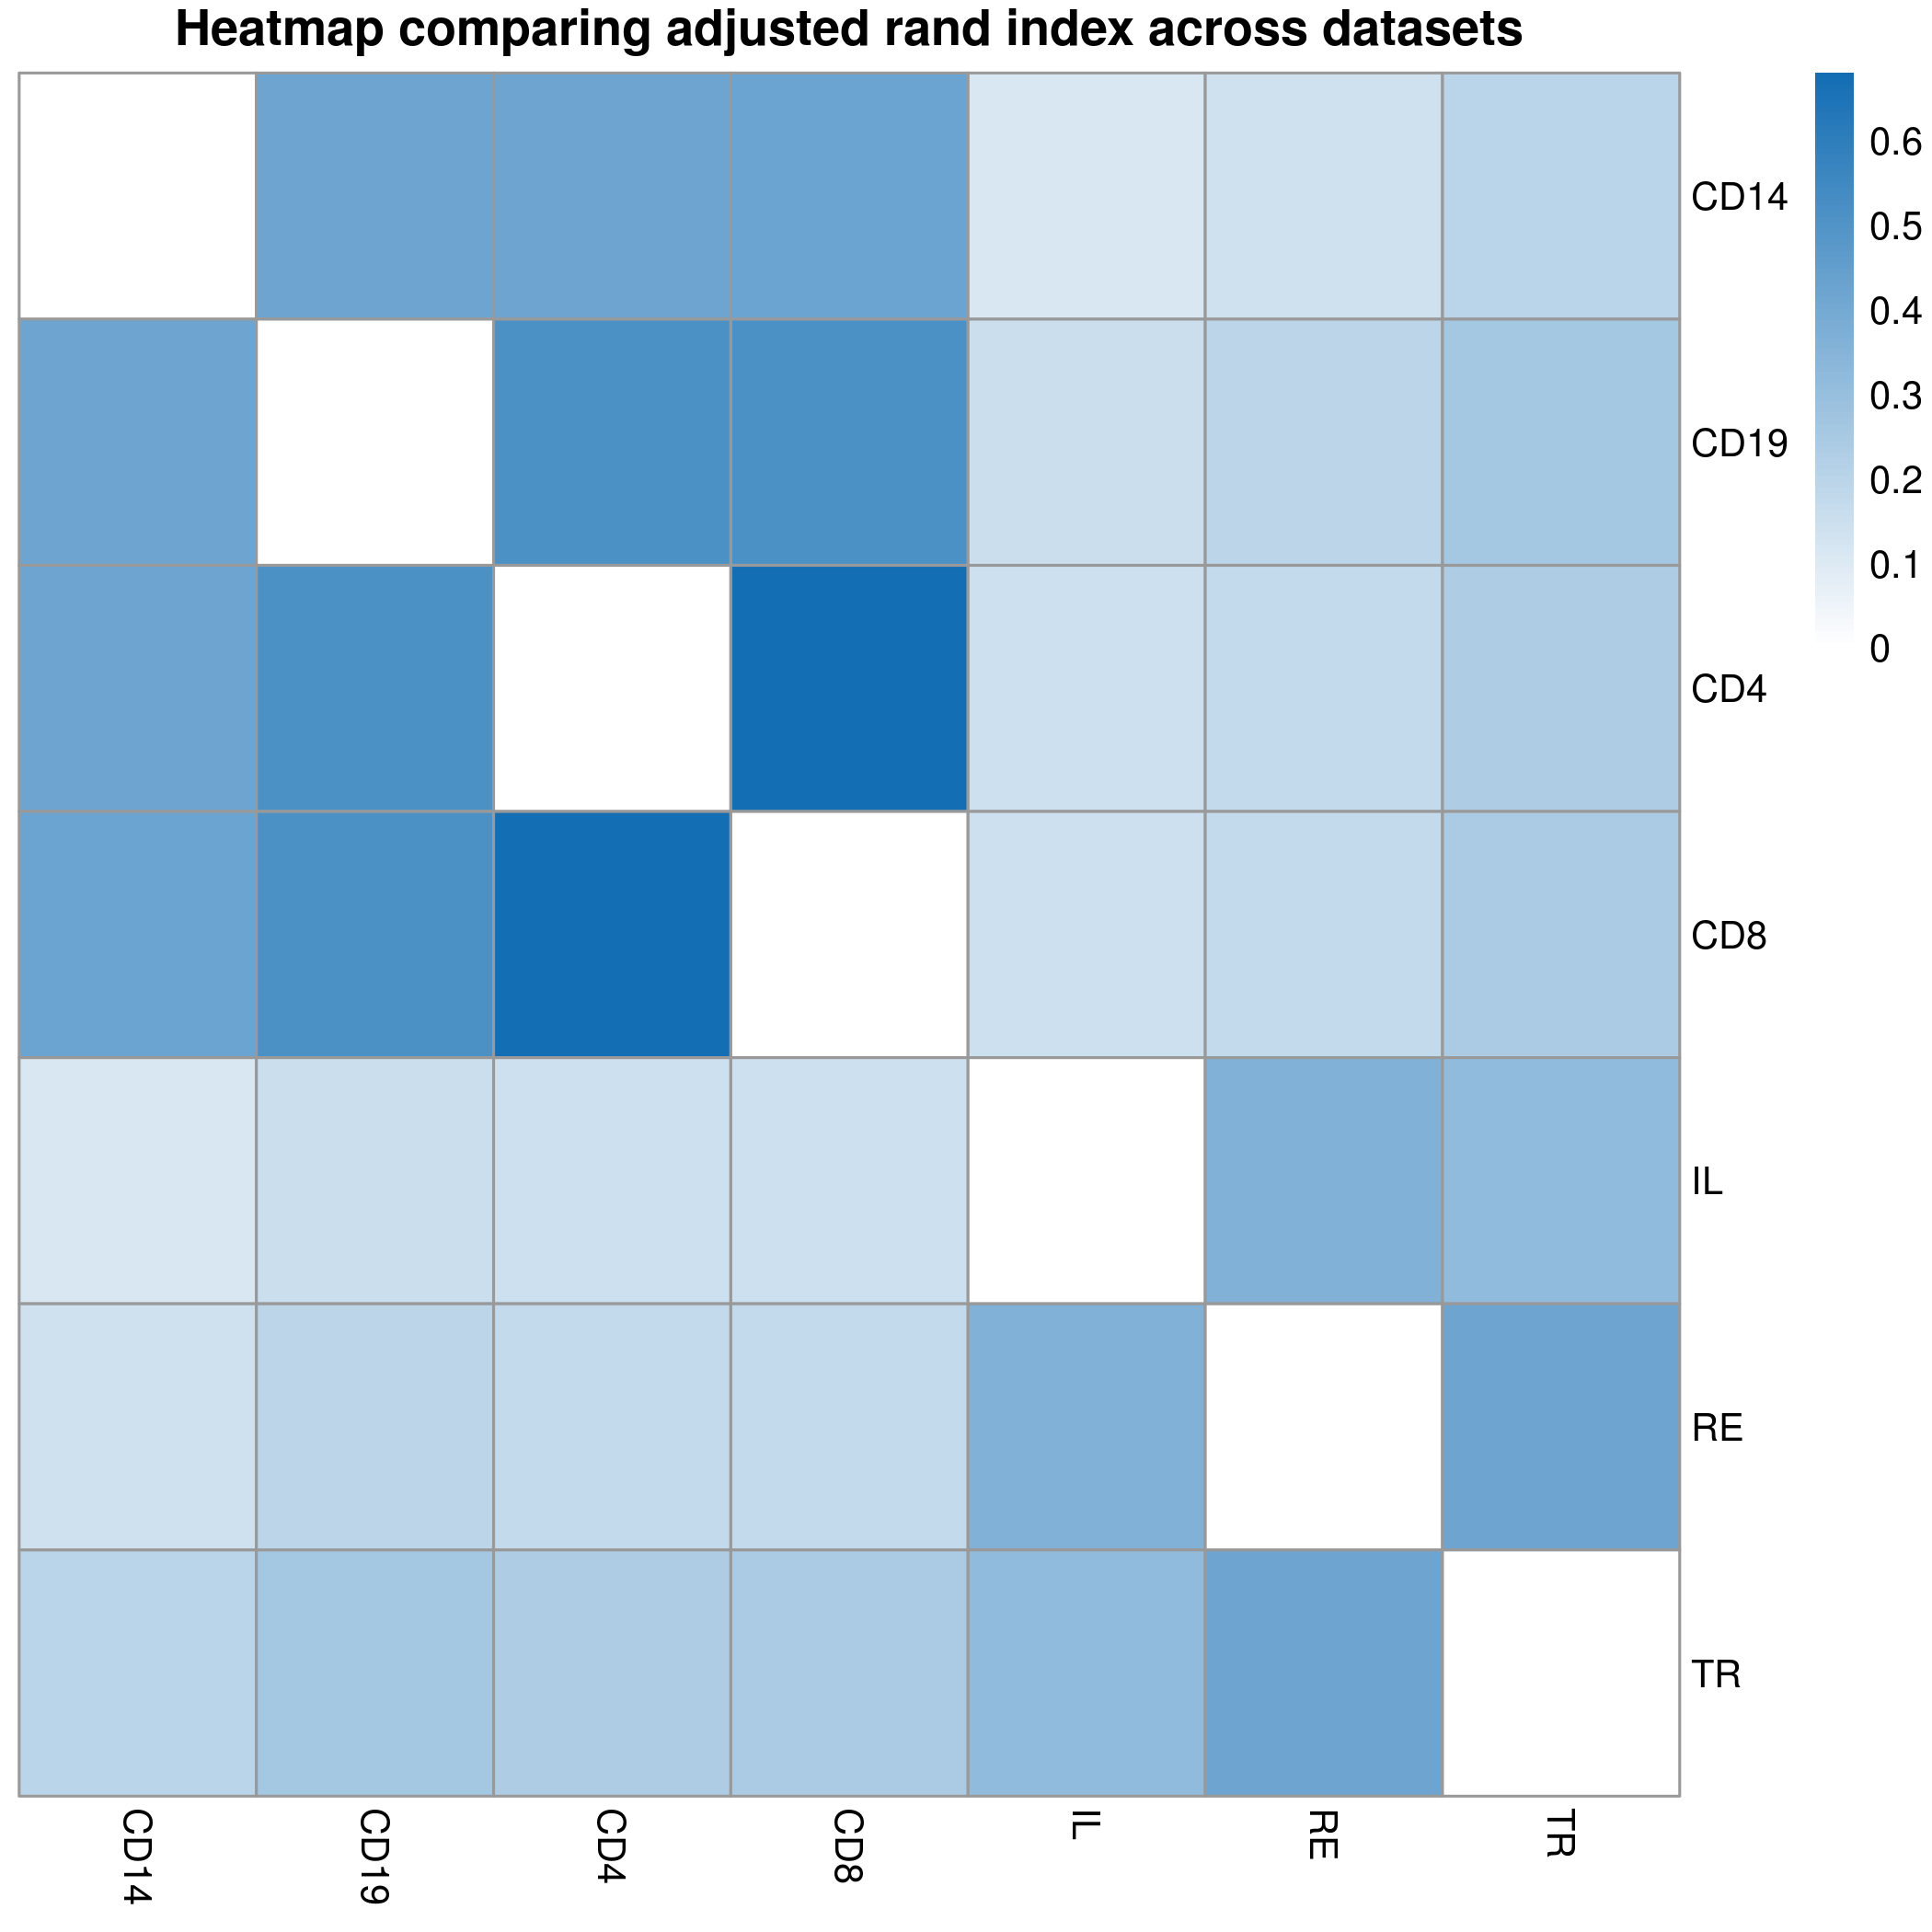
\includegraphics[scale=0.75]{Images/Biology_data/Set_1000/All_datasets/Arandi_heatmap.png}
		\caption{CEDAR Case 2: Heatmap of the mean adjusted Rand index comparing the clustering across datasets for each seed. Again one can see that the immune cells form a distinct group from the intestinal samples.}
		\label{fig:results:cedar_2:mdi_adj_rand_ind_heatmap}
	\end{figure}
	
%	\newpage
	
	\begin{figure}[h]
		\centering
		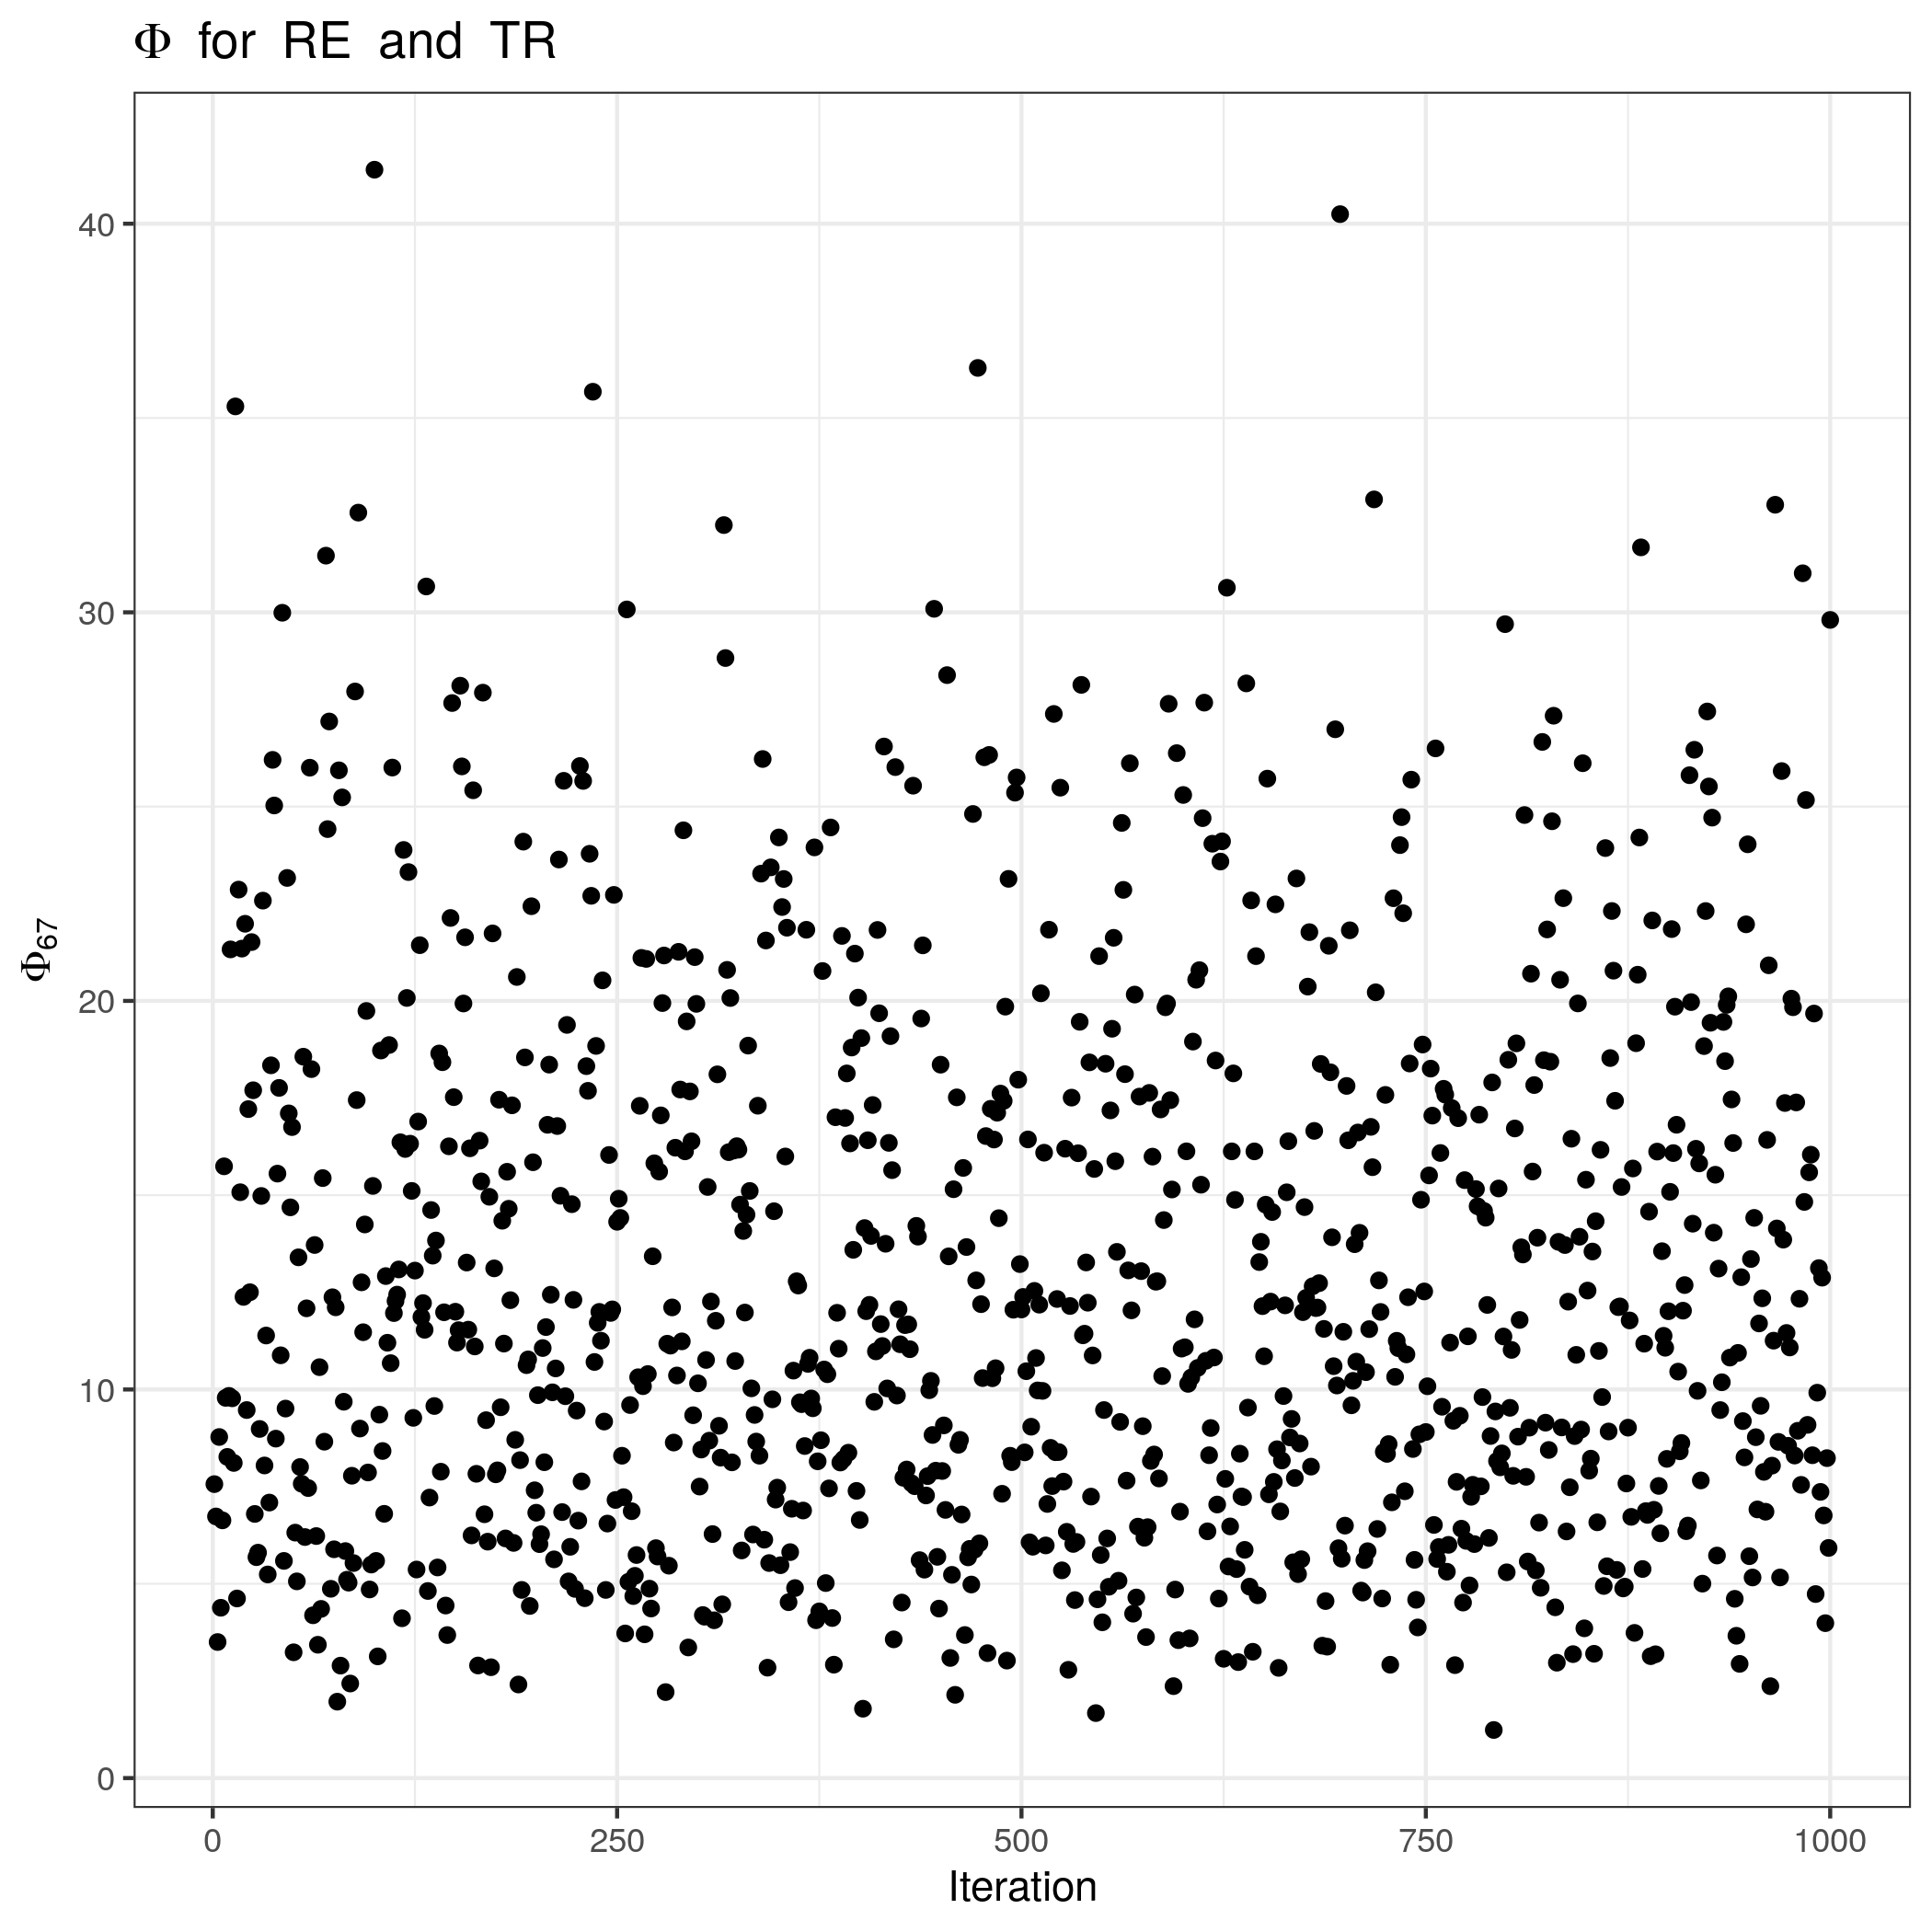
\includegraphics[scale=0.75]{Images/Biology_data/Set_1000/All_datasets/Phi_series_plots/file_1_Phi_67.png}
		\caption{CEDAR Case 2: Plot of the $\phi_{67}$ values across all seeds, between the RE and TR datasets (note that the high values indicate a high clustering correlation).}
		\label{fig:results:cedar_2:mdi_re_tr_phi_series_plot}
	\end{figure}
	
%	\newpage
	
	\begin{figure}[h]
		\centering
		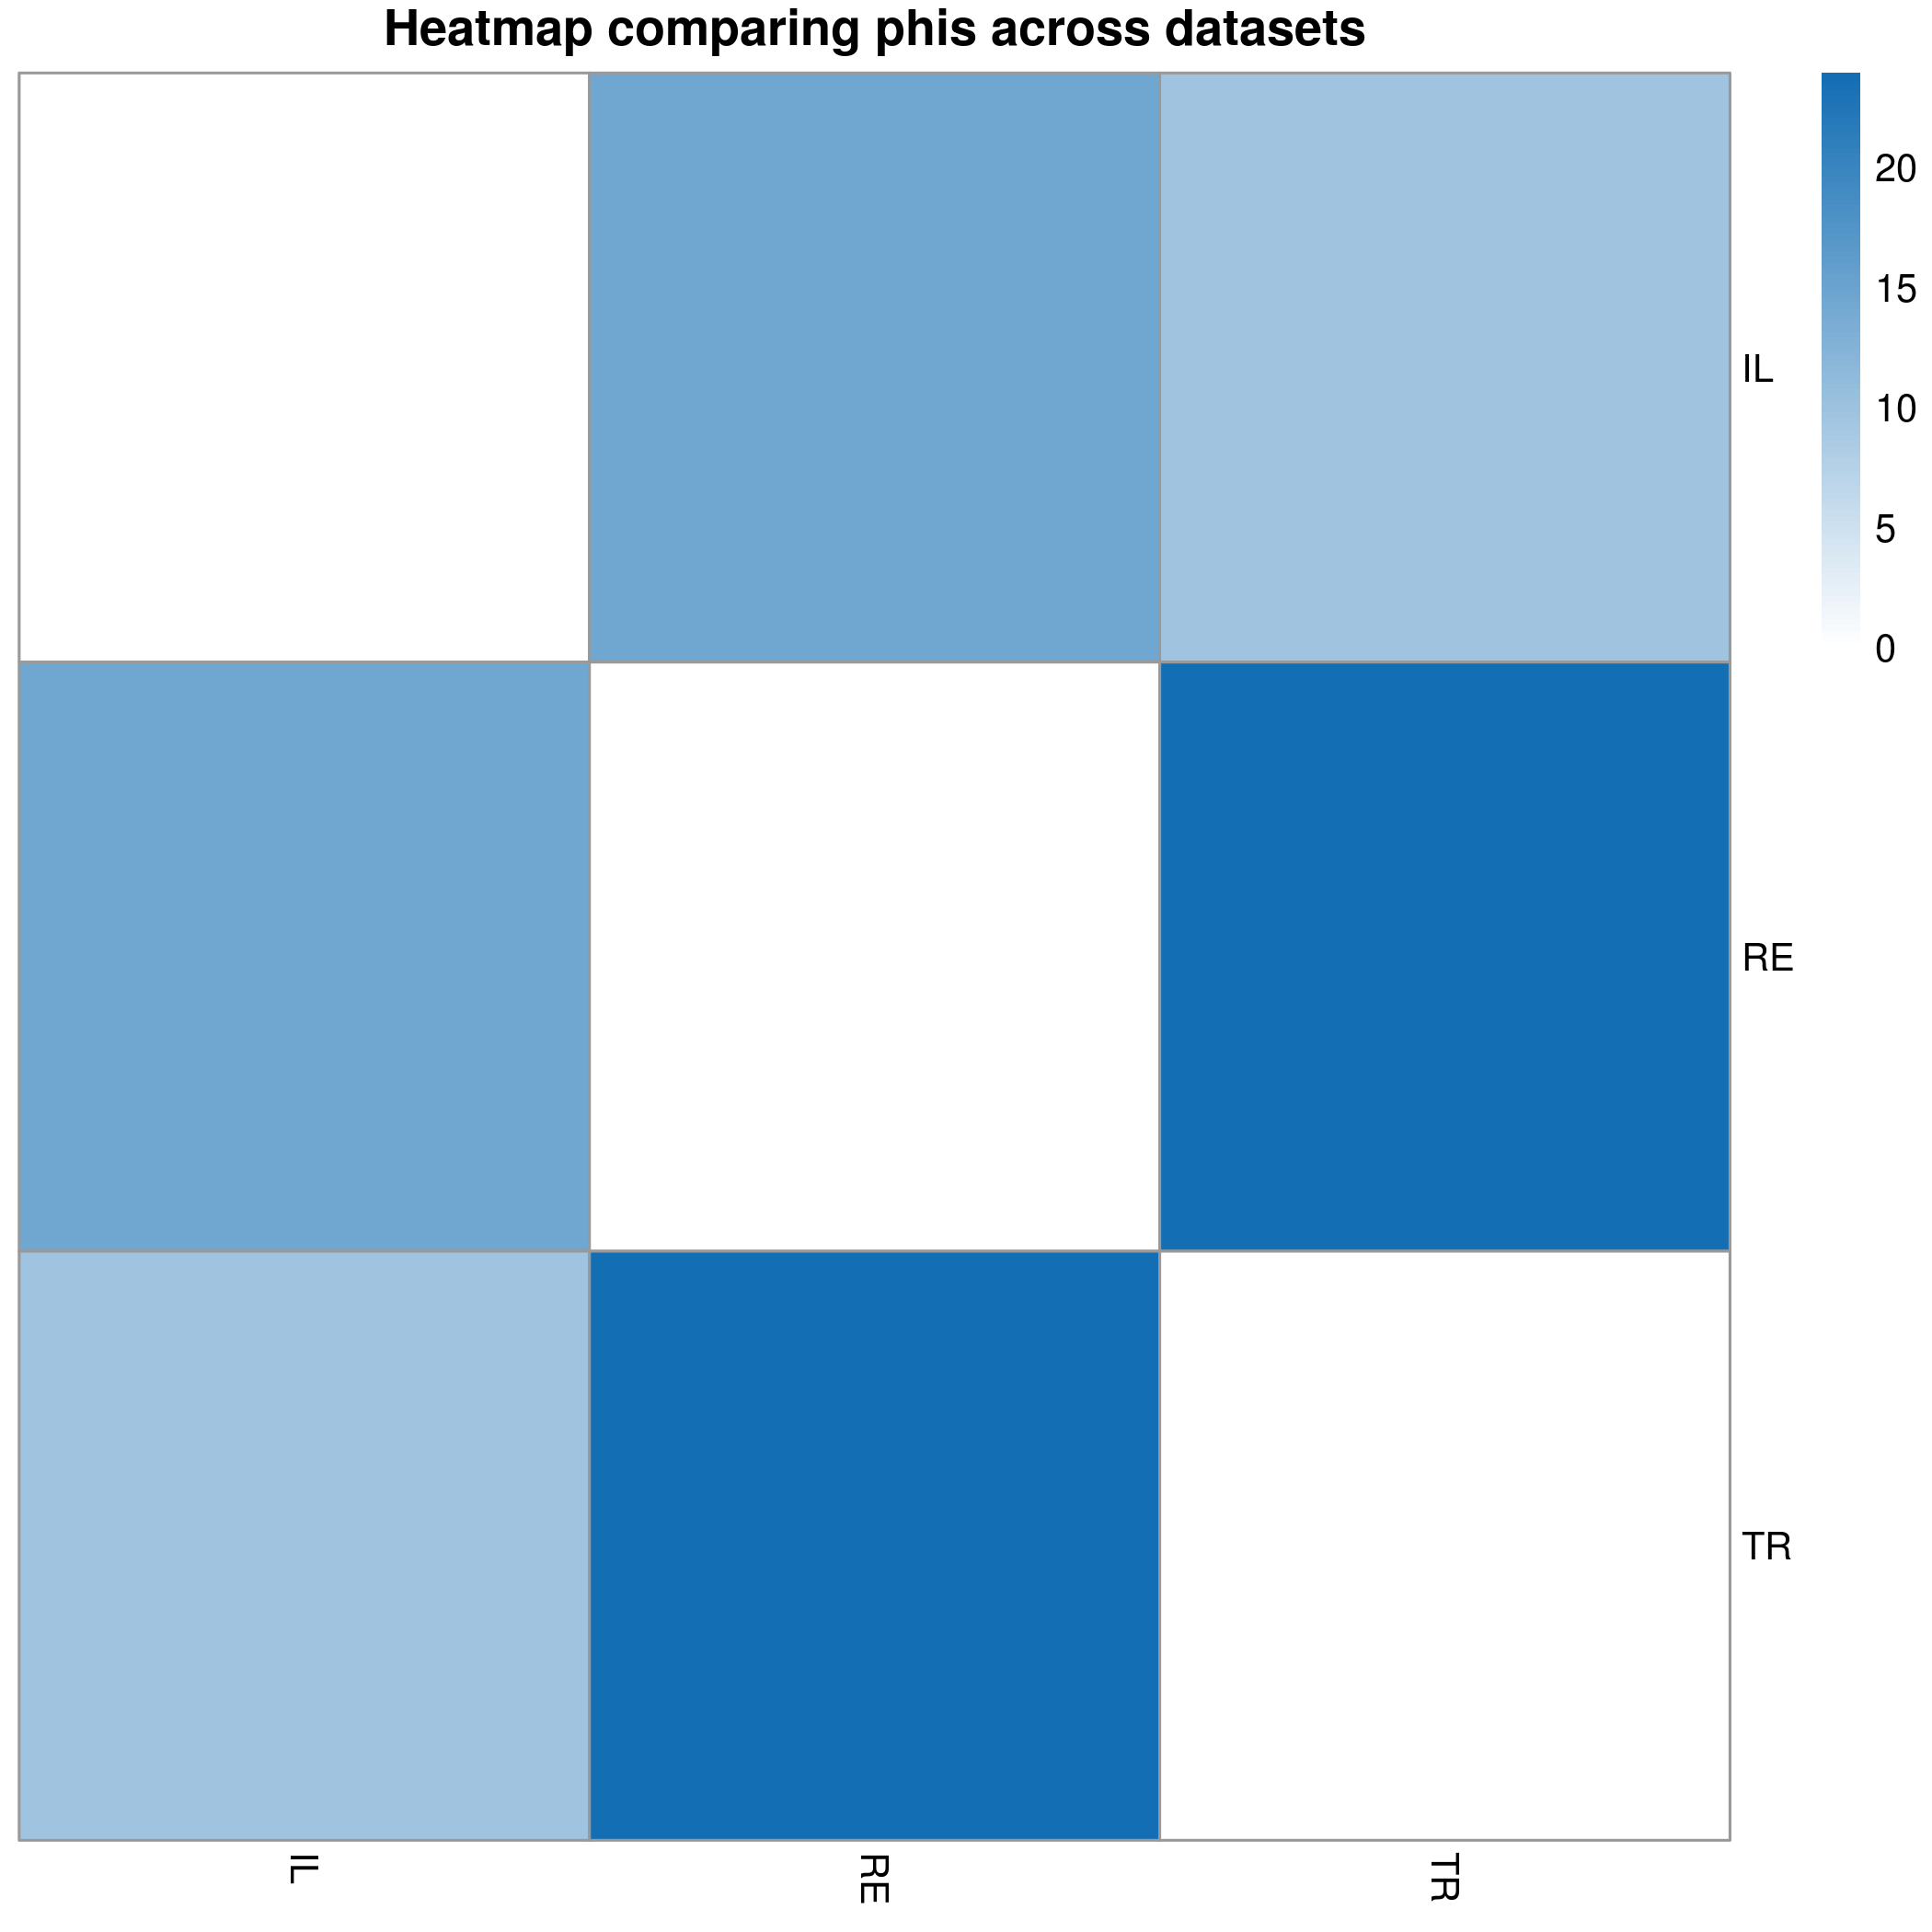
\includegraphics[scale=0.75]{Images/Biology_data/Set_1000/All_datasets/Phi_heatmap_1.png}
		\caption{CEDAR Case 2: Plot of the mean $\phi_{ij}$ values across all seeds, between the all datasets.}
		\label{fig:results:cedar_2:mdi_phi_heatmap}
	\end{figure}
	
%	\newpage
	
	
	%		\begin{figure}[h]
	%		\centering
	%		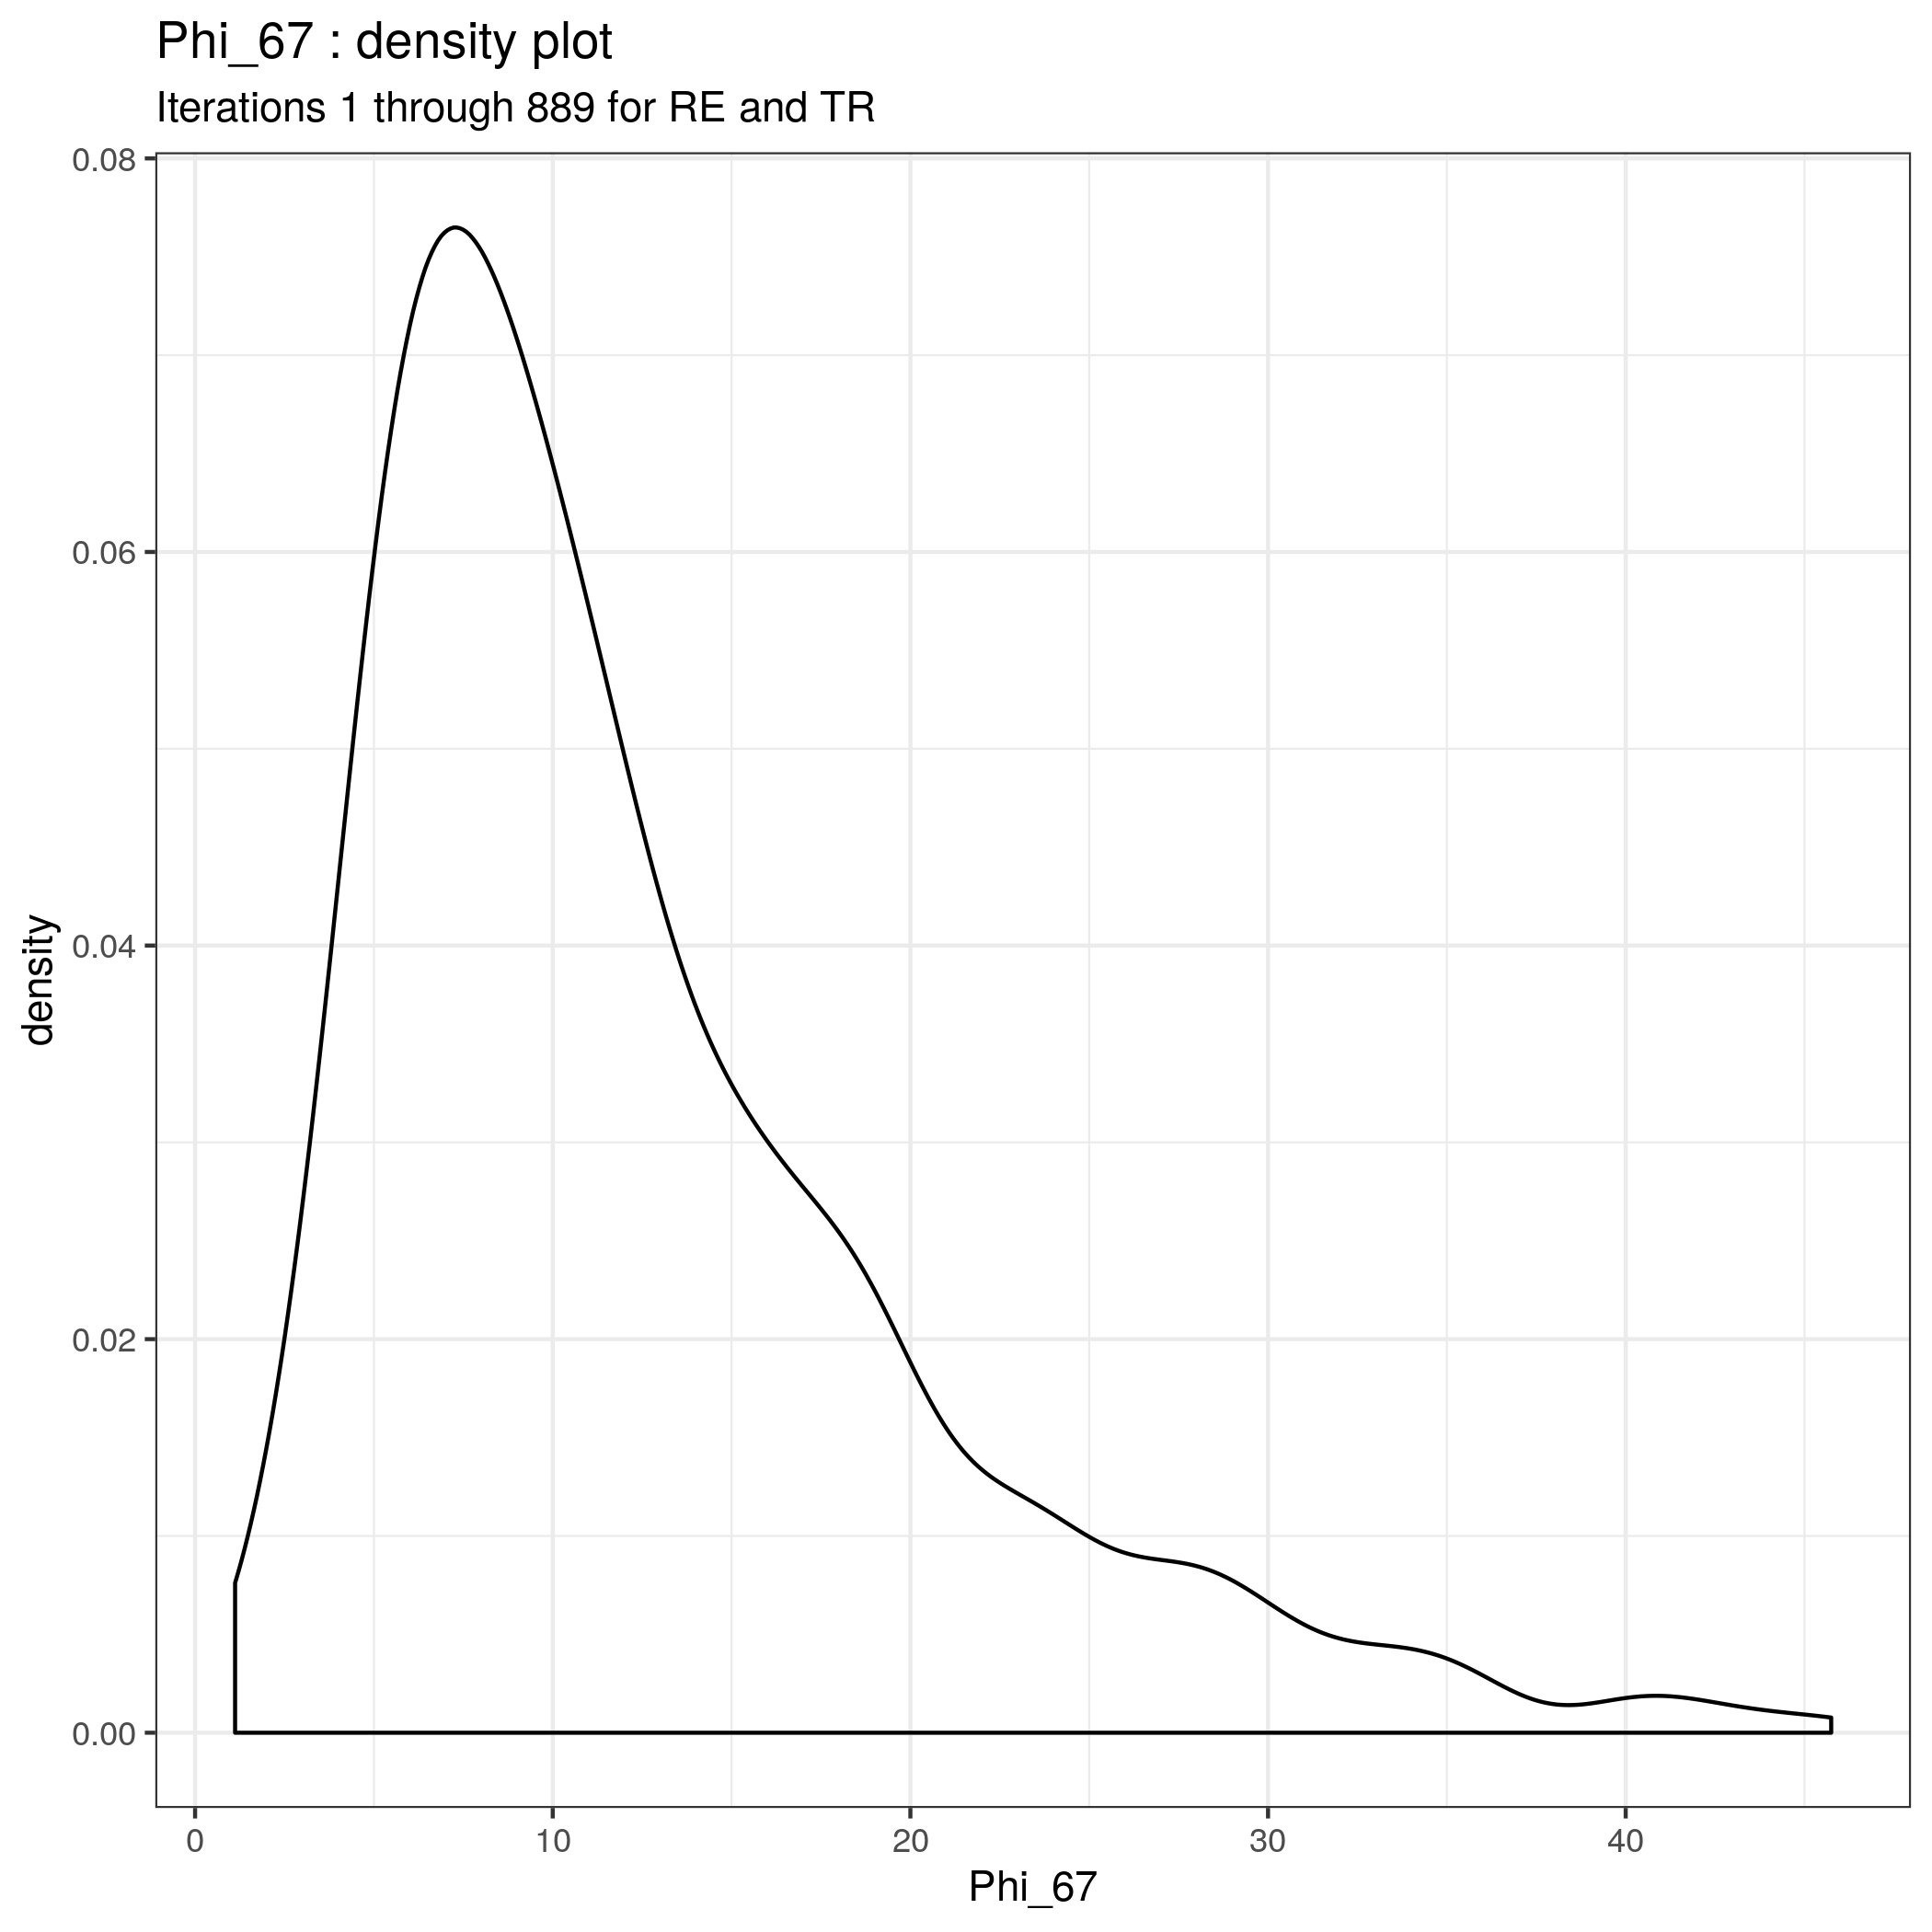
\includegraphics[scale=0.75]{Images/Biology_data/All_datasets/Phi_density_plots/Phi_67_density_plot.png}
	%		\caption{Plot of the distribution $\phi_{67}$ values across all seeds, between the RE and TR datasets (note that the high values indicate a high clustering correlation).}
	%		\label{fig:results:cedar_2:mdi_re_tr_phi_density_plot}
	%	\end{figure}
	%
	%	\newpage
	
	\begin{figure}[h]
		\centering
		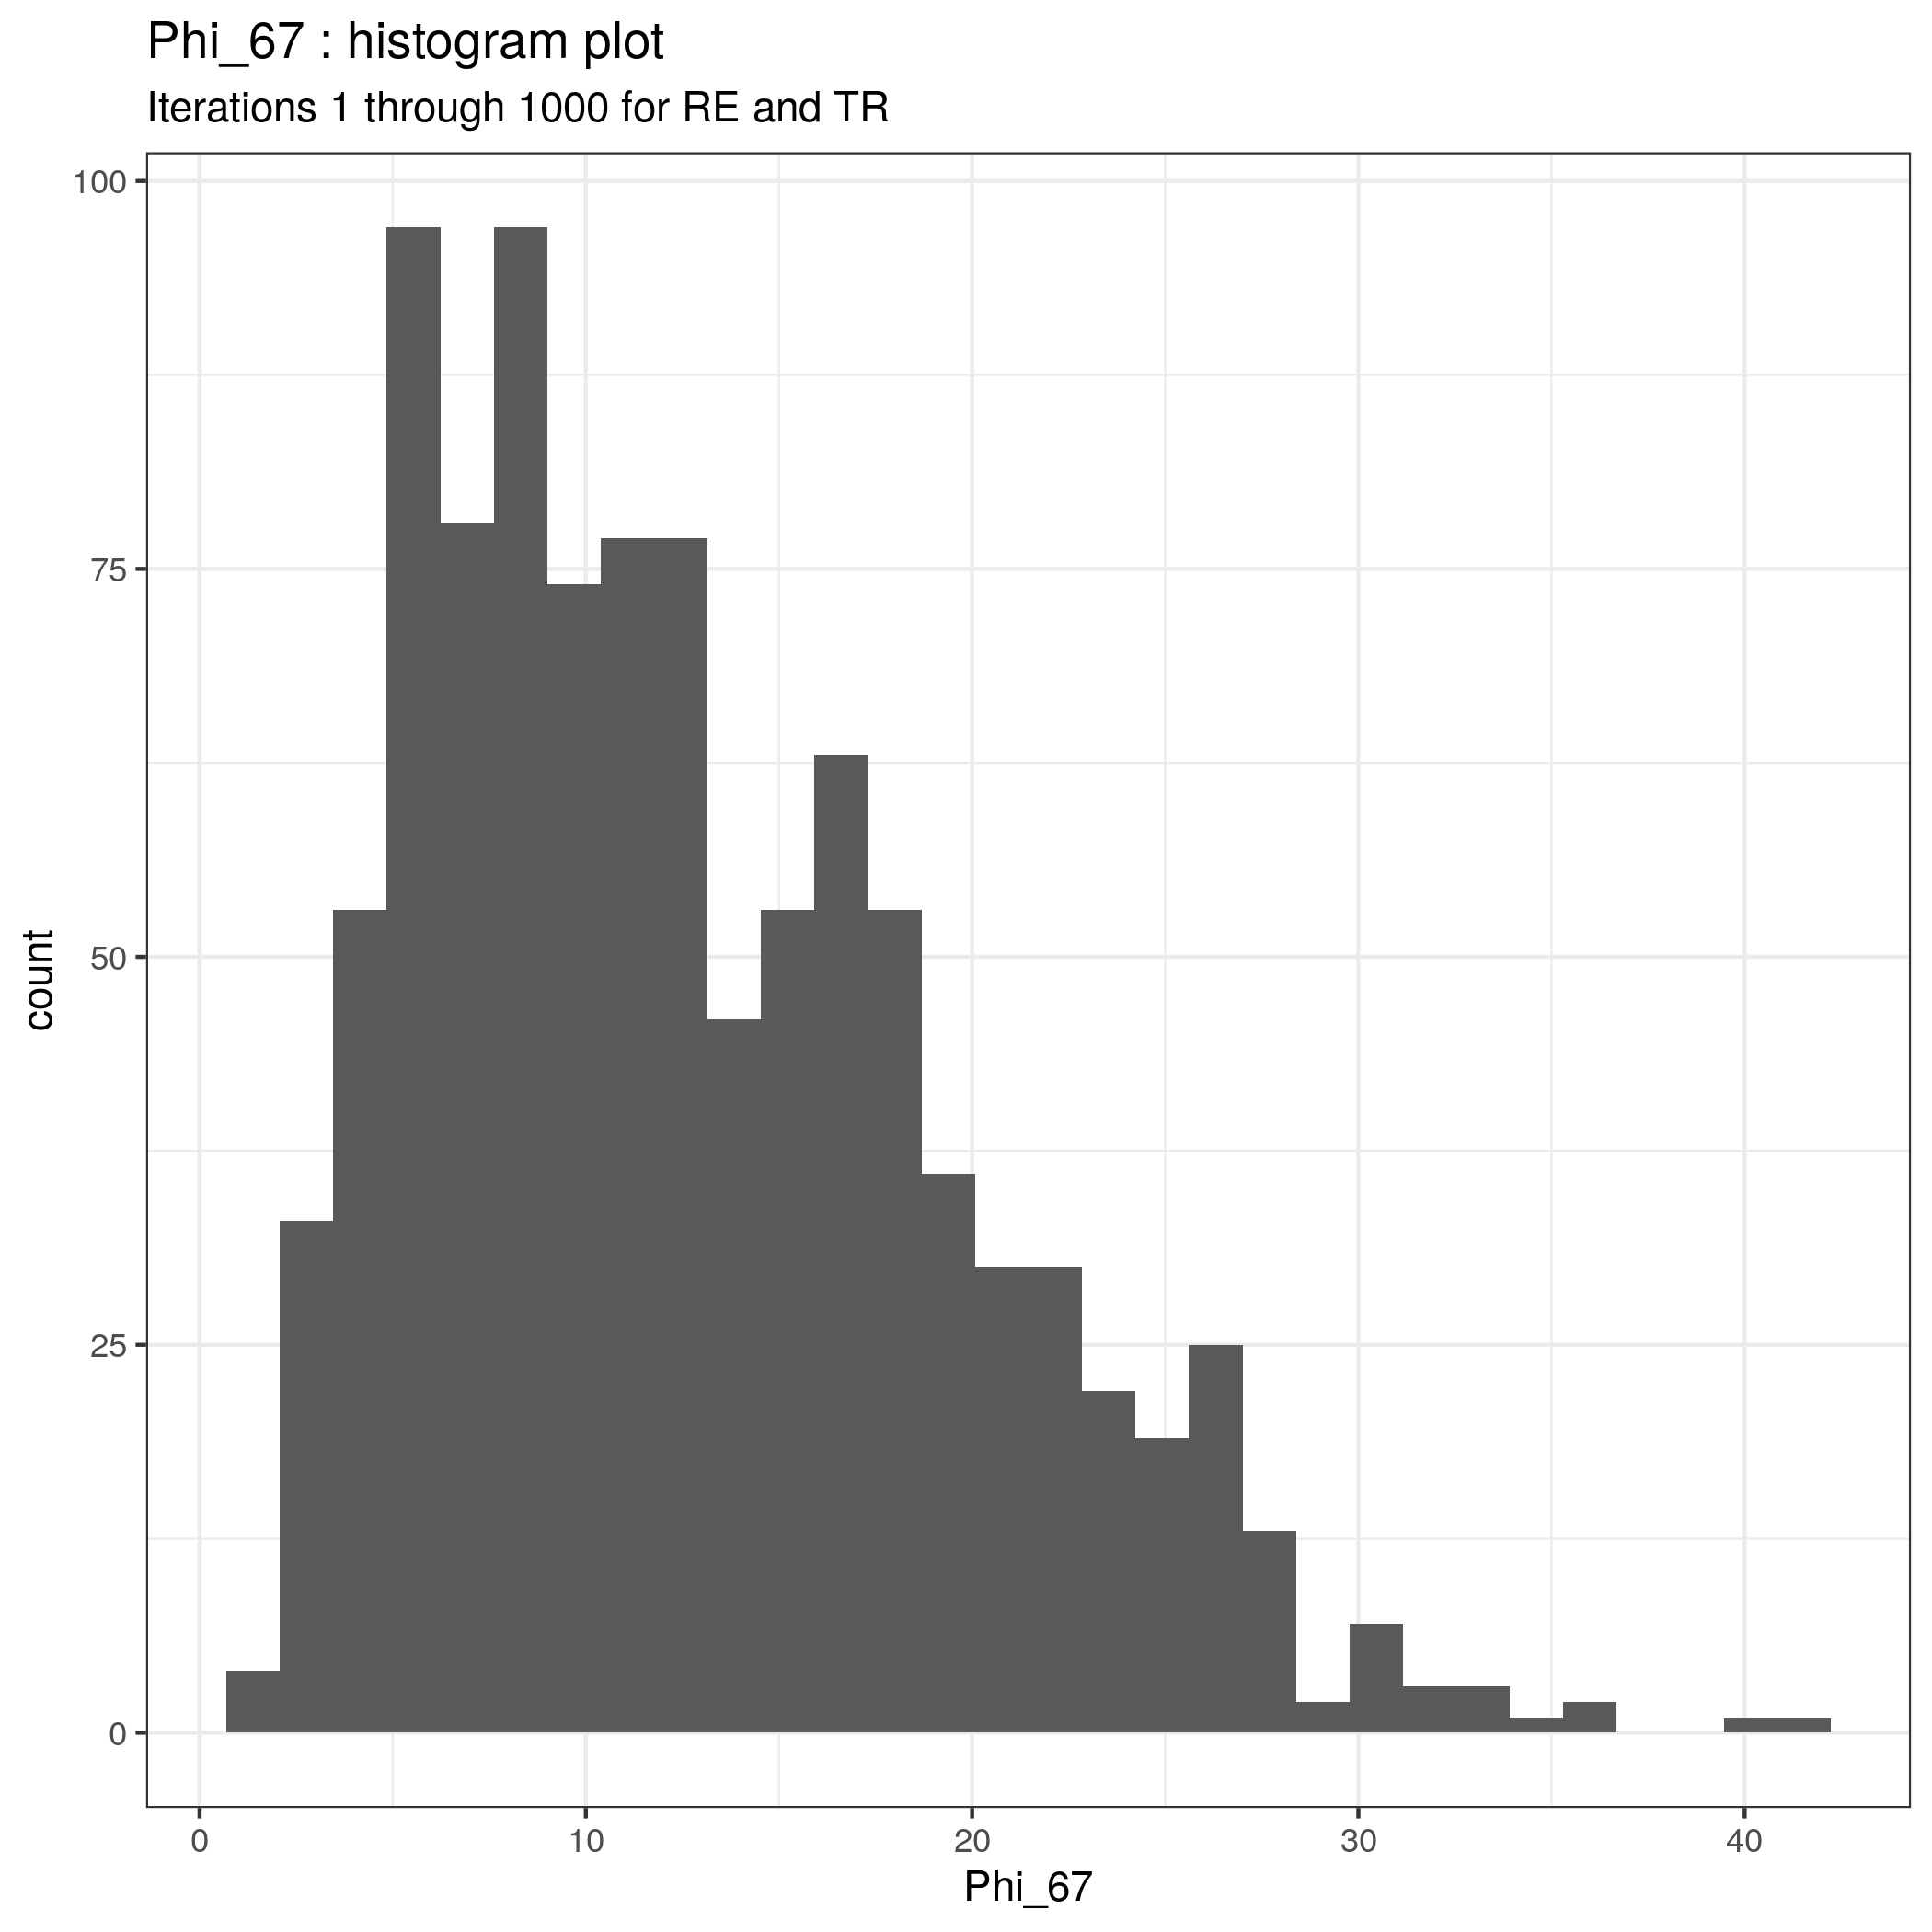
\includegraphics[scale=0.75]{Images/Biology_data/Set_1000/All_datasets/Phi_histograms/Phi_67_histogram_plot.png}
		\caption{CEDAR Case 2: Histogram of the distribution of $\phi_{67}$ values across seeds(between the RE and TR datasets).}
		\label{fig:results:cedar_2:mdi_re_tr_phi_histogram}
	\end{figure}
	
%	\newpage
	
	
	\begin{figure}[h]
		\centering
		\includegraphics[scale=0.75]{Images/Biology_data/Set_1000/All_datasets/Cluster_series_plots/CD4.png}
		\caption{CEDAR Case 2: Plot of the number of clusters present in each seed for the CD4 dataset.}
		\label{fig:results:cedar_2:mdi_cd4_number_clusters_plot}
	\end{figure}
	
%	\newpage
	
	\begin{figure}[h]
		\centering
		\includegraphics[scale=0.75]{Images/Biology_data/Set_1000/All_datasets/Mass_parameter_plots/CD4.png}
		\caption{CEDAR Case 2: Plot of the mass parameter ($\alpha$) for the Dirichlet process for the CD4 dataset of MDI.}
		\label{fig:results:cedar_2:mdi_cd4_mass_parameter_plot}
	\end{figure}
	
%	\newpage
	
	
	
	\begin{figure}[h]
		\centering
		\includegraphics[scale=0.75]{Images/Biology_data/Set_1000/All_datasets/Similarity_matrices/similarity_matrix_CD4.png}
		\caption{CEDAR Case 2: Heatmap of the PSM for the CD4 dataset from the consensus clustering of MDI.}
		\label{fig:results:cedar_2:mdi_cd4_psm}
	\end{figure}
	
%	\newpage
	
	\begin{sidewaysfigure}[h]
		\centering
		\includegraphics[scale=0.5]{Images/Biology_data/Set_1000/All_datasets/Comparison_expression_clustering_correlation/CD4.png}
		\caption{CEDAR Case 2: Heatmap of the PSM for the CD4 dataset from the consensus clustering of MDI. Again the PSM mirrors structure present in the correlation matrix and many of the blocks in the PSM have corresponding blocks of structure in the standardised expression data.}
		\label{fig:results:cedar_2:mdi_cd4_psm_expr_cor}
	\end{sidewaysfigure}
	

%	\newpage

	The signal of clustering for the IBD KEGG pathway can be seen in two different tissues in figures \ref{fig:results:cedar_2:mdi_il_ibd_alignment_prob_distn} and \ref{fig:results:cedar_2:mdi_cd14_ibd_alignment_prob_distn}. It can be seen that in IL there is encouraging signal that the structure of the IBD pathways is uncovered to a non-random degree, whereas it is not uncovered at all in the CD14 dataset.
%	
%	\begin{enumerate}
%		\item The annotated PSMs of the dataset and the subset of data from the pathway was plotted (see figure \ref{fig:results:cedar_2:mdi_il_ibd_psm_cor} for an example of this); and
%		\item The distribution of the mean pairwise alignment probability and the the mean pairwise alignment probability of the $m$ genes from the pathway of interest (for an example, please see figures \ref{fig:results:cedar_2:mdi_il_ibd_alignment_prob_distn} and \ref{fig:results:cedar_2:mdi_cd14_ibd_alignment_prob_distn} for a comparison across datasets).
%	\end{enumerate}
	
	\begin{sidewaysfigure}[h]
		\centering
		\includegraphics[scale=0.75]{Images/Biology_data/Set_1000/All_datasets/Heatmaps/KEGG_INFLAMMATORY_BOWEL_DISEASE/IL_comp_psm_corr.png}
		\caption{CEDAR Case 2: Heatmap of the PSM and expression data for the IBD probes for the IL dataset from the consensus clustering of MDI.}
		\label{fig:results:cedar_2:mdi_il_ibd_psm_cor}
	\end{sidewaysfigure}
	
	
	\begin{figure}[h]
		\centering
		\includegraphics[scale=0.75]{Images/Biology_data/Set_1000/All_datasets/Mean_alignment_probability/IL_KEGG_INFLAMMATORY_BOWEL_DISEASE.png}
		\caption{CEDAR Case 2: Plot of the distribution of the mean probability of pairwise alignment for a random sample of probes genes with a dashed line indicating the mean probability of pairwise alignment for the IBD associated probes in the IL dataset.}
		\label{fig:results:cedar_2:mdi_il_ibd_alignment_prob_distn}
	\end{figure}
	
	\begin{figure}[h]
		\centering
		\includegraphics[scale=0.75]{Images/Biology_data/Set_1000/All_datasets//Mean_alignment_probability/CD14_KEGG_INFLAMMATORY_BOWEL_DISEASE.png}
		\caption{CEDAR Case 2: Plot of the distribution of the mean probability of pairwise alignment for a random sample of probes genes with a dashed line indicating the mean probability of pairwise alignment for the IBD associated probes in the CD14 dataset.}
		\label{fig:results:cedar_2:mdi_cd14_ibd_alignment_prob_distn}
	\end{figure}
%	\newpage
	
	\section{Conclusion}
%	PLAN FOR CONCLUSION
%	\begin{itemize}
%		\item Consensus clustering does explore the same space as MDI attempts to cover;
%		\item Appears robust to different values of $n_{iter}$;
%		\item Consensus clustering is a powerful tool for exploring multi-modal data;
%		\item Consensus clustering is fast and accurate;
%		\item GENE stuff?
%		\item future work - more datasets; include sick people, more people; try different clustering methods within consensus clustering
%	\end{itemize}
	
%	It can be seen that when MDI does converge and successfully samples from the posterior space (section \ref{sec:results:case_1}), consensus clustering samples from the same space and performs very similarly in terms of describing the underlying structure of the data. The results in section \ref{sec:results:case_2} show that even when MCMC methods struggle to converge, consensus clustering offers a description of the space of interest. Consensus clustering captures multiple modes in a similar distribution to the space described across all chains of MDI (see figure \ref{fig:gen_data_case_2_collapsed_violin_plot}). The consensus clustering also appears to be robust in terms of the number of iterations used in each individual chain (each consensus clustering length performs identically). As each chain used in consensus clustering is independent of the others the problem is embarrassingly parallel; therefore 1,000 chains of 500 iterations is far quicker to run in parallel than a single long chain. This means that even when multi-modality is not expected to be an issue for MCMC methods that consensus clustering is a useful alternative based purely on the reduction in run-times in a parallel environment.
	
	Between sections \ref{sec:results:case_1} and \ref{sec:results:case_2} I have shown that this consensus clustering approach to inference provides significant computational gains over traditional MCMC approaches when one has access to an environment enabling parallel chains while still enabling meaningful clustering structures to be uncovered and assessments of uncertainty to be performed. Moreover, this approach is better able to explore complex multi-modal posterior distributions as a consequence of the vast number of parallel chains that are used to establish the consensus. Thus this inferential method has many of the advantages of Bayesian inference (the use of priors, quantification of error, interpretability) but overcomes the limitations of convergence and speed. It should be noted that these limits of Bayesian clustering methods apply to any field where high dimensional, multi-modal datasets are used and thus this implementation of consensus clustering has applications ranging beyond the case studies described here. I have also shown that consensus clustering is robust to chain length (figure \ref{fig:gen_data_case_2_collapsed_violin_plot}) within the cases tested here, but this may need further testing.
	
%	The combination of these results encourages the claim that consensus clustering is a quick, robust solution to the problem of scaling Bayesian clustering methods generally and of multi-modality specifically. Consensus clustering produces a more accurate description of the posterior distribution than any single chain is capable of in a multi-modal high dimensional space within a realistic number of iterations; thus this implementation has many of the advantages of Bayesian inference (the use of priors, quantification of error) but overcomes the limitations of convergence and speed. It should be noted that these limits of Bayesian clustering methods apply to any field where high dimensional, multi-modal datasets are used and thus this implementation of consensus clustering has applications ranging beyond the case studies described here.
	
	When applied to the CEDAR data case studies, consensus clustering has positive results. First, it can be applied in this case when individual Bayesian methods are not feasible (as MDI cannot be run across the datasets within the computational constraints of this project and even if it could one can see from the individual mixture models (figure  \ref{fig:results:cedar_1:cd14_bayes_mixture_model_comp}) that it is not likely to converge). The agreement between the PSM and the correlation matrix that can be seen in figure \ref{fig:results:cedar_1:mdi_cd4_psm_expr_cor} is reassuring - it shows that the clustering imposed is in line with the data. Furthermore, the results displayed in figures \ref{fig:results:cedar_1:mdi_cd4_inostiol_alignemnt_prob_distn} and \ref{fig:results:cedar_2:mdi_il_ibd_alignment_prob_distn} are encouraging. It looks like my model has successfully uncovered some of the structure of a pathway. This is supported by the difference between the PSM entries for the associated probes compared to the non-pathway probes as can be seen in figure \ref{fig:results:cedar_1:mdi_cd4_inostiol_psm_violin}. However, it should be noted that this validation of the model is expected to be limited as co-expression data is unlikely to contain all the information required to describe a KEGG pathway - thus I am not surprised to see that the model uncovers only some of the pathway structure as the entire structure is not likely to be present in the dataset.
	
	The contrast between figures \ref{fig:results:cedar_2:mdi_il_ibd_alignment_prob_distn} and \ref{fig:results:cedar_2:mdi_cd14_ibd_alignment_prob_distn} is also encouraging of the thesis that tissue annotation is important for pathways. The IBD pathway is uncovered with some success in the IL dataset, but none at all in the CD14 dataset. This is as one might expect - the intestinal samples are pieces of tissue, thus there are a range of cells present here, including tissue-resident immune cells. These tissue-resident immune cells, which mediate IBD, are in the environment where IBD manifests. Due to this I expect to see the IBD pathway present here, whereas the immune cell datasets could be from any location, and thus I do not expect to see a tissue specific disease pathway present; a result that may be seen in figure \ref{fig:results:cedar_2:mdi_cd14_ibd_alignment_prob_distn}. Furthermore, comparison of figures \ref{fig:results:cedar_1:mdi_cd4_inostiol_alignemnt_prob_distn},  \ref{fig:results:cedar_1:mdi_cd8_inostiol_alignemnt_prob_distn} and \ref{fig:results:cedar_1:mdi_il_inostiol_alignemnt_prob_distn} indicates that the inositol phosphate metabolism pathway is not specific to a single tissue (admittedly the signal is weaker in the last of these figures), as one might expect for such a broad pathway. This is encouraging as the tissue / cell-type specificity does appear to be present, and present in keeping with prior expectations.
	
	We can see the benefits of using MDI models in figures \ref{fig:results:cedar_1:mdi_mixture_model_comp_tr}, \ref{fig:results:cedar_1:mdi_adj_rand_ind_heatmap}, \ref{fig:results:cedar_1:mdi_phi_heatmap}, \ref{fig:results:cedar_2:mdi_adj_rand_ind_heatmap} and \ref{fig:results:cedar_2:mdi_phi_heatmap}. The first, figure \ref{fig:results:cedar_1:mdi_mixture_model_comp_tr}, shows that MDI is more confident in allocating probes together. This is due to the additional information available to the model through the other datasets. The other plots, figures \ref{fig:results:cedar_1:mdi_adj_rand_ind_heatmap}, \ref{fig:results:cedar_1:mdi_phi_heatmap}, \ref{fig:results:cedar_2:mdi_adj_rand_ind_heatmap} and \ref{fig:results:cedar_2:mdi_phi_heatmap}, show that MDI can be used to quantify the similarity in structure of the datasets, something individual mixture models cannot do. As one would expect, these show that the three colon samples are quite similar and the CD datasets are similar, with little information shared across these sets of datasets. We can also see that the CD4 and CD8 datasets are highly correlated (the high mean $\phi$ value across seeds), as one would expect from two types of T lymphocyte. RE and TR are more similar to each other than to IL, as might be expected from figure \ref{fig:colon_location} (if IL and RE had been distinctly more similar that might have raised some concerns).
	
	My conclusions from this project can be summarised by the following points:
	\begin{enumerate}
		\item Consensus clustering offers a computationally tractable approximation of Bayesian inference when a parallel environment is available; 
		\item There is evidence suggesting that tissue / cell-type specific annotation of gene sets is a relevant addition to existing gene sets; and
		\item MDI is a powerful tool for clustering across datasets offering unique advantages such as quantification of similarity and the ability to move towards independent mixture models if there is no common structure.
	\end{enumerate} 
	
	\section{Future work}
	With regards to consensus clustering there are several outstanding questions worth investigating:
	\begin{enumerate}
		\item How many seeds are required to explore the modes present?
		\item How short can the individual chains be?
		\item How does this form of inference extend to other clustering methods?
	\end{enumerate}
	The first two points would be expected to depend on characteristics of the dataset in question, but some suggestions could be drawn from well designed simulations.
	
	For the application of annotating gene sets with tissue and cell-type specific information, the encouraging results from section \ref{sec:results:cedar} suggest further work to integrate tissue-specific information into definitions of gene sets could be rewarding. Different datasets might also be of use; for instance datasets with repeated measurements of expression over time or proteomics datasets might offer more information of interest to define gene sets (and thus overcoming some of the limitations of this analysis). One of the advantages of MDI is that the different datasets used do not have to all be the same kind of data as long as the row names are the same; even different types of data, such as categorical, can be integrated in the clustering. This, in combination with the fact that MDI allows the $\phi_{ij}$ parameter to go to 0 if there is no correlation, means that MDI appears to be the natural tool to use in such analysis. Thanks to these features one can use datasets one thinks might be relevant without a fear of disrupting the signal present in the other datasets. Due to the improved tractability of consensus clustering the computational constraints are less severe which might otherwise severely limit the inclusion of another dataset if one was using a purely Bayesian inference of MDI.
	
	
	
	
	
%	\newpage
%	\begin{table}[]
%		\centering
%		\begin{tabular}{l|CCCCCC}
%			Case   & \alpha_1 & \alpha_2 & \alpha_3 & \phi_{12}   & \phi_{13}   & \phi_{23} \\
%			\hline
%			Case 1 & 0.951            & 0.912            & 0.705            & 0.534   & 0.893   & 0.705   \\
%			Case 1 & 0.804            & 0.787            & 0.516            & 0.563   & 0.605   & 0.787   \\
%			Case 1 & 0.627            & 0.784            & 0.592            & 0.534   & 0.789   & 0.985   \\
%			Case 1 & 0.870             & 0.912            & 0.534            & 0.686   & 0.951   & 0.743   \\
%			Case 1 & 0.516            & 0.534            & 0.985            & 0.686   & 0.705   & 0.951   \\
%			Case 1 & 0.893            & 0.534            & 0.951            & 0.985   & 0.705   & 0.743   \\
%			Case 1 & 0.790	& 0.787            & 0.867            & 0.705   & 0.992   & 0.888   \\
%			Case 1 & 0.563            & 0.534            & 0.592            & 0.789   & 0.572   & 0.534   \\
%			Case 1 & 0.516            & 0.784            & 0.985            & 0.627   & 0.985   & 0.893   \\
%			Case 1 & 0.743            & 0.892            & 0.892            & 0.743   & 0.787   & 0.572  
%		\end{tabular}
%		\caption{Test statistic from Geweke diagnostic of convergence for each parameter for case 1 chains.}
%	\label{table:geweke_case_1}
%	\end{table}
%
%		\begin{table}[]
%		\centering
%		\begin{tabular}{l|CCCCCC}
%			Case   & \alpha_1 & \alpha_2 & \alpha_3 & \phi_{12}   & \phi_{13}   & \phi_{23} \\
%			\hline
%			Case 2 & 0.867            & 0.787            & 0.951            & 0.821   & 0.87    & 0.789   \\
%			Case 2 & 0.787            & 0.516            & 0.847            & 0.743   & 0.686   & 0.951   \\
%			Case 2 & 0.787            & 0.627            & 0.516            & 0.870    & 0.87    & 0.897   \\
%			Case 2 & 0.705            & 0.789            & 0.795            & 0.592   & 0.985   & 0.605   \\
%			Case 2 & 0.787            & 0.870             & 0.893            & 0.516   & 0.787   & 0.985   \\
%			Case 2 & 0.867            & 0.795            & 0.87             & 0.784   & 0.893   & 0.870    \\
%			Case 2 & 0.534            & 0.534            & 0.516            & 0.870    & 0.705   & 0.563   \\
%			Case 2 & 0.605            & 0.969            & 0.784            & 0.897   & 0.534   & 0.516   \\
%			Case 2 & 0.743            & 0.705            & 0.592            & 0.827   & 0.892   & 0.883   \\
%			Case 2 & 0.563            & 0.534            & 0.893            & 0.563   & 0.592   & 0.787  
%		\end{tabular}
%	\caption{Test statistic from Geweke diagnostic of convergence for each parameter for case 2 chains.}
%	\label{table:geweke_case_2}
%	\end{table}
%
%
%\begin{table}[]
%	\begin{tabular}{l|CCCCCC}
%		Case   & \alpha_1 & \alpha_2 & \alpha_3 & \phi_{12}   & \phi_{13}   & \phi_{23} \\
%		\hline
%		Case 1 & 0.157            & -0.256           & -1.129           & -1.905  & -0.325  & 1.098   \\
%		Case 1 & -0.66            & -0.819           & 2.288            & 1.587   & -1.368  & 0.792   \\
%		Case 1 & 1.307            & -0.888           & 1.499            & -1.766  & 0.732   & 0.042   \\
%		Case 1 & -0.484           & -0.263           & 1.779            & -1.22   & 0.152   & 0.984   \\
%		Case 1 & -2.115           & -1.837           & 0.062            & 1.212   & -1.104  & -0.164  \\
%		Case 1 & -0.331           & 1.748            & 0.195            & 0.031   & 1.148   & 0.984   \\
%		Case 1 & -0.705           & 0.762            & 0.549            & 1.166   & -0.011  & -0.411  \\
%		Case 1 & -1.607           & 1.977            & 1.478            & 0.722   & -1.538  & 1.725   \\
%		Case 1 & -2.139           & -0.88            & 0.029            & 1.3     & -0.086  & -0.353  \\
%		Case 1 & 1.026            & 0.378            & -0.382           & 0.974   & -0.779  & 1.548   \\
%		Case 2 & -0.542           & -0.768           & 0.161            & -0.632  & -0.458  & 0.74    \\
%		Case 2 & 0.781            & 2.296            & 0.587            & 0.966   & -1.204  & 0.189   \\
%		Case 2 & -0.775           & -1.302           & 2.52             & 0.482   & -0.477  & -0.292  \\
%		Case 2 & -1.076           & -0.717           & -0.68            & 1.43    & 0.078   & -1.377  \\
%		Case 2 & -0.768           & -0.514           & -0.333           & -2.164  & 0.792   & -0.06   \\
%		Case 2 & 0.535            & -0.685           & 0.45             & -0.884  & 0.336   & -0.464  \\
%		Case 2 & -1.99            & 1.768            & -2.202           & 0.457   & 1.088   & -1.602  \\
%		Case 2 & -1.392           & 0.12             & 0.902            & -0.303  & 1.816   & -2.591  \\
%		Case 2 & -0.993           & 1.133            & 1.434            & 0.617   & -0.377  & 0.427   \\
%		Case 2 & -1.588           & 1.798            & 0.316            & 1.589   & -1.429  & -0.85  
%	\end{tabular}
%\end{table}
%
%
%\begin{table}[]
%	\begin{tabular}{l|CCCCCC}
%		Case   & \alpha_1 & \alpha_2 & \alpha_3 & \phi_{12}   & \phi_{13}   & \phi_{23} \\
%		\hline
%		Case 1 & 0.157            & -0.256           & -1.129           & -1.905  & -0.325  & 1.098   \\
%		Case 1 & -0.66            & -0.819           & 2.288            & 1.587   & -1.368  & 0.792   \\
%		Case 1 & 1.307            & -0.888           & 1.499            & -1.766  & 0.732   & 0.042   \\
%		Case 1 & -0.484           & -0.263           & 1.779            & -1.22   & 0.152   & 0.984   \\
%		Case 1 & -2.115           & -1.837           & 0.062            & 1.212   & -1.104  & -0.164  \\
%		Case 1 & -0.331           & 1.748            & 0.195            & 0.031   & 1.148   & 0.984   \\
%		Case 1 & -0.705           & 0.762            & 0.549            & 1.166   & -0.011  & -0.411  \\
%		Case 1 & -1.607           & 1.977            & 1.478            & 0.722   & -1.538  & 1.725   \\
%		Case 1 & -2.139           & -0.88            & 0.029            & 1.3     & -0.086  & -0.353  \\
%		Case 1 & 1.026            & 0.378            & -0.382           & 0.974   & -0.779  & 1.548  
%	\end{tabular}
%\end{table}
%
%
%\begin{table}[]
%	\begin{tabular}{l|CCCCCC}
%		Case   & \alpha_1 & \alpha_2 & \alpha_3 & \phi_{12}   & \phi_{13}   & \phi_{23} \\
%		\hline
%		Case 2 & -0.542           & -0.768           & 0.161            & -0.632  & -0.458  & 0.74    \\
%		Case 2 & 0.781            & 2.296            & 0.587            & 0.966   & -1.204  & 0.189   \\
%		Case 2 & -0.775           & -1.302           & 2.52             & 0.482   & -0.477  & -0.292  \\
%		Case 2 & -1.076           & -0.717           & -0.68            & 1.43    & 0.078   & -1.377  \\
%		Case 2 & -0.768           & -0.514           & -0.333           & -2.164  & 0.792   & -0.06   \\
%		Case 2 & 0.535            & -0.685           & 0.45             & -0.884  & 0.336   & -0.464  \\
%		Case 2 & -1.99            & 1.768            & -2.202           & 0.457   & 1.088   & -1.602  \\
%		Case 2 & -1.392           & 0.12             & 0.902            & -0.303  & 1.816   & -2.591  \\
%		Case 2 & -0.993           & 1.133            & 1.434            & 0.617   & -0.377  & 0.427   \\
%		Case 2 & -1.588           & 1.798            & 0.316            & 1.589   & -1.429  & -0.85  
%	\end{tabular}
%\end{table}



%	\section{Results}
%	
%	To check if the algorithm ran and as an initial exploration of the data, we implemented the steps described in \ref{list:methods} applying MDI to all 9 datasets. This was done twice - on the first occasion probes missing from a dataset or containing NAs were dropped (resulting in a total dataset of 4,964 probes in each dataset) and on the second occasion using an imputed value of 0 for missing probes (on this occasion we dropped probes that had NAs in some columns in all datasets reducing the dataset from 18,523 to 18,517 probes).
%	
%	The algorithm was capable of running for 10,000 iterations with a thinning factor of 25 over both these set of data.
%	
%	We used the modal clustering as the predicted clustering as the labels became fixed and did not vary for the majority of iterations. We did not use the clustering implied by the PSM as the clusters were very defined and thus the uncertainty captured by the PSM was not necessary for the predicted clustering. Furthermore, the computational cost of calculating the PSM, particularly for the larger dataset, was quite high (the PSM is a $n \times n$ matrix).
%	
%	MDI begins with 50 clusters (as an approximation of a Dirichlet process - note that we can change the number of clusters present). In the 9 datasets the number of occupied clusters stabilised around 10 (ranging from 8 - 13).
%	
%	We inspected the resulting clusters using the \emph{pheatmap} package \citep{KoldepheatmapPrettyHeatmaps2018} in R \citep{RCoreTeamLanguageEnvironmentStatistical2018}.
%	
%	\begin{figure}[h]
%	%	\centering
%		\includegraphics[scale=1.0]{Images/Initial_analysis/mdi_1_heatmap-1.png}
%		\caption{Predicted clusters for MDI applied to 9 datasets for common probes with datasets as columns and probes as rows.}
%		\label{fig:naive_mdi_reduced}
%	\end{figure}
%
%	We can see from figure \ref{fig:naive_mdi_reduced} that some genes cluster across all datasets (the beige band about 0.25 along the vertical axis). Between the combination of a visual inspect and the hierarchical clustering visible in the tree at the top of figure \ref{fig:naive_mdi_reduced} combined with the information in figure \ref{fig:naive_mdi_reduced_phi_heatmap}, one can see that the platelets behave significantly differently to the other datasets - very few rows align with other datasets. We can see that we have 4 distinct groups of datasets here:
%	\begin{enumerate} \label{list:datasets_naive_mdi_reduced}
%		\item CD14, CD4 and CD8;
%		\item IL and RE;
%		\item CD15, CD19 and TR; and
%		\item PLA.
%	\end{enumerate}
%
%	\begin{figure}[h]
%		\centering
%		\includegraphics[scale=0.75]{Images/Initial_analysis/Phi_heatmap_1.png}
%		\caption{Mean $\phi$ value between datasets across iterations. $\phi$ can be considered a measure of similarity between datasets - the greater $\phi_{i,j}$ is, the more correlated the clustering in datasets $i$ and $j$ is.}
%		\label{fig:naive_mdi_reduced_phi_heatmap}
%	\end{figure}
%	
%	However, there is too much information in figure \ref{fig:naive_mdi_reduced} for serious analysis and we must use subsets of the data to better understand the information contained here. Based on the clusters of datasets mentioned in \label{list:datasets_naive_mdi_reduced}, we visualise the clustering in these groups.
%	
%	From figures \ref{fig:naive_mdi_reduced_il_tr_cluster} and \ref{fig:naive_mdi_reduced_cd14_cd4_cd8_cluster}, one can see that inspecting the clusters in subsets of the datasets makes it easier to see similarity in clustering.
%	
%	
%%	\begin{figure}[h]
%%		%	\centering
%%		\includegraphics[scale=1.0]{Images/Initial_analysis/sim_heatmaps-1.png}
%%		\caption{Predicted clusters for MDI applied to 9 datasets for common probes with datasets as columns and probes as rows.}
%%		\label{fig:naive_mdi_reduced}
%%	\end{figure}
%
%	\begin{figure}[h]
%		%	\centering
%		\includegraphics[scale=1.0]{Images/Initial_analysis/sim_heatmaps-2.png}
%		\caption{Predicted clusters for MDI applied to 9 datasets for common probes with datasets as columns and probes as rows.}
%		\label{fig:naive_mdi_reduced_il_tr_cluster}
%	\end{figure}
%	
%	\begin{figure}[h]
%		%	\centering
%		\includegraphics[scale=1.0]{Images/Initial_analysis/sim_heatmaps-3.png}
%		\caption{Predicted clusters for MDI applied to 9 datasets for common probes with datasets as columns and probes as rows.}
%		\label{fig:naive_mdi_reduced_cd14_cd4_cd8_cluster}
%	\end{figure}
%
%	\begin{figure}[h]
%	%	\centering
%	\includegraphics[scale=1.0]{Images/Initial_analysis/mdi_2_heatmap-1.png}
%	\caption{Predicted clusters for MDI applied to 9 datasets for all probes.}
%	\label{fig:naive_mdi_full}
%\end{figure}
	
	\newpage



%	\bibliographystyle{abbrv}
	\bibliographystyle{plainnat}
%	\bibliographystyle{ieeetr}
	
%	\bibliography{thesis}
	\bibliography{thesis_ref_better}
	

\newpage

\appendix
%\section{Data generation explained}

\section{Gibbs sampling} \label{sec:additional_theory:sub_sec:gibbs_sampler}
Gibbs sampling is based on the concept of \emph{Monte Carlo integration} and \emph{Markov chains}. It is a special case of the \emph{Metropolis-Hastings algorithm}. Gibbs sampling is used to sample directly from the posterior distribution of the model's random variables. I briefly describe the emphasized terms below before describing Gibbs sampling in more detail.

\subsubsection{Monte Carlo integration}
The original Monte Carlo method was developed as a means to solving integrals by use of random number generation \citep{MetropolisMonteCarloMethod1949}.

Suppose there is some complex integral one wishes to solve on some interval, $(a,b)$:

\begin{align}
\int_a^b h(x) dx
\end{align}
If one can decompose $h(x)$ into the product of some more simple function $f(x)$ and a probability density $p(x)$ where both are defined over $(a,b)$, it can then be stated:

\begin{align} \label{monte_carlo_basis}
\int_a^bh(x)dx = \int_a^bf(x)p(x)dx = \mathbb{E}_{p(x)}\left[f(x)\right]
\end{align}
It is assumed that one can approximate this expectation of $f(x)$ over $p(x)$ by drawing $N$ random variables $x = (x_1,\ldots,x_N)$ from $p(x)$ (by the Law of Large Numbers); thus \eqref{monte_carlo_basis} becomes:

\begin{align} \label{monte_carlo_integration}
\int_a^bh(x)dx = \mathbb{E}_{p(x)}\left[f(x)\right] \approx \frac{1}{N}\sum_{i=1}^Nf(x_i)
\end{align}
This is \emph{Monte Carlo integration}.

\subsubsection{Markov chains}
Consider a random variable $X$ observed at discrete times $t = (t_0,\ldots,t_n)$, with the observation at $t_i$ denoted $X(t_i)$. Let $S$ be the state space of possible values $X$ can take. $X$ is said to have the \emph{Markov property} if the transition probabilities between states depend only on the current state, i.e. for any states $s_i, s_j, s_k \in S$:

\begin{align}
\mathbb{Pr}(X(t_{n+1}) = s_j | X(t_0) = s_k, \ldots, X(t_n) = s_i) = \mathbb{Pr}(X(t_{n+1}) = s_j | X(t_n) = s_i) 
\end{align}
Thus prediction depends only on the information in the present; the process is said to be memory-less as the past does not affect future outcomes. In this case  $X$ is referred to as a \emph{Markov process}. A \emph{Markov chain} refers to a sequence of random variables $(X_0,\ldots,X_n)$ generated by a Markov process.

Let $\mathbf{P}$ be the matrix of $|S| \times |S|$ where entry $(i,j)$ is the transition probability from state $s_i$ to $s_j$. Define the $n$-step transition probability $p_{ij}^n$ as the probability that the process is in state $s_j$ given it was in state $s_i$ at a remove of $n$ steps, i.e.:

\begin{align}
p_{ij}^n = \mathbb{Pr}(X(t_{i+n} = s_j | X(t_i) = s_i)
\end{align}
A Markov chain is said to be \emph{irreducible} if $p_{ij}^n > 0 \; \forall \; i,j \in \mathbb{N}$. This means that there always exists a possible path from any state $s_i$ to every other state $s_j$. If this is true the states are said to communicate. If the number of steps between two states is not required to be the multiple of some integer than the chain is considered aperiodic.

For some state $s \in S$ denote $ \mathbb{Pr}(X(t_{n+1}) = s)$ by $\pi_s$. The chain has the \emph{reversible} property if for any states $x, y \in S$ the detailed balance \eqref{eqn:detailed_balance} holds:

\begin{align} \label{eqn:detailed_balance}
\mathbb{Pr}(X(t_{n+1}) = x | X(t_n) = y)  \pi_x  =  \mathbb{Pr}(X(t_{n+1}) = y | X(t_n) = x) \pi_y
\end{align}
This is sufficient condition for a unique, stationary distribution. That is the probability of being in any given state for the process is independent of the starting condition given sufficient time and the transition probabilities have approached some limiting value. 


More formally, a stationary distribution, $\pi$, is a row-vector with $|S|$ entries defined by:
\begin{align}
\pi_j &\geq 0 \: \forall \: j \in (1,\ldots,|S|) \\
\sum_{j=1}^{|S|}\pi_j &= 1
\end{align}
That is invariant under the operation of the transition matrix $\mathbf{P}$ upon it. That is:
\begin{align} \label{eqn:stationary_distribution}
\pi = \pi\mathbf{P}
\end{align}
Thus the distribution, $\pi$, remains unchanged in the Markov chain as time progresses.

%If the detailed balance holds, then $\mathbf{P}$ goes to a limiting distribution under the number of transitions, $n$:
%\begin{align}
%\lim_{n\to\infty}\mathbf{P}^n &= \begin{bmatrix}
%1 \\
%1 \\
%\vdots \\
%1
%\end{bmatrix} \pi
%\end{align}
If for any initial state $\pi_0$, the chain has the property:
\begin{align}
\lim_{n\to\infty} \pi_0 \mathbf{P}^n = \pi
\end{align}
For some transition matrix $\mathbf{P}$ and stationary distribution $\pi$, then the chain is said to converge to $\pi$. Once the chain is sampling from $\pi$, then as this distribution is stationary, the samples drawn should be independent of the previous draws as can be seen in \eqref{eqn:stationary_distribution}. For this reason auto-correlation is one of the tests of convergence within a Markov chain.

%Thus one can converge in which case one has achieved stationarity and the transition matrix being drawn from is independent of the initial transition matrix.

\subsubsection{Markov-Chain Monte Carlo methods}
Markov-Chain Monte Carlo (MCMC) methods developed as a method to obtain samples from some complex distribution $p(x)$ for the decomposition suggested in \eqref{monte_carlo_basis}. The goal in the following is to draw samples from some distribution $p(\theta)$ where there is some distribution $f(\theta)$ such that:

\begin{align}
p(\theta) = \frac{f(\theta)}{K} 
\end{align}
For some constant $K$ where $K$ may not be known and is often difficult to compute.

The Metropolis algorithm \citep{MetropolisMonteCarloMethod1949, MetropolisEquationStateCalculations1953} generates a sequence of draws from $p(\theta)$ using the following steps:

\begin{enumerate}
	\item Initialise with some arbitrary value $\theta_0$ with the condition that $f(\theta_0) > 0$ and also choose some probability density $q(\theta_1|\theta_2)$ as the \emph{jumping distribution} or \emph{proposal density}. For the Metropolis algorithm one demands that this is symmetric (i.e. $q(\theta_1 | \theta_2) = q(\theta_2 | \theta_1)$).
	\item For each iteration, $t$:
	\begin{enumerate}
		\item Using the current value $\theta_{t-1}$, sample a candidate point, $\theta^*$, from  $q(\theta^* | \theta_{t-1})$.
		\item Calculate the \emph{acceptance ratio} for the new value $\theta^*$:
		\begin{align}
		\alpha = \frac{p(\theta^*)}{p(\theta_{t-1})} = \frac{f(\theta^*)}{f(\theta_{t-1})}
		\end{align}
		Note that as the proportionality constant is the same for all $\theta$ that this is an equivalence rather than proportional relationship.
		\item Accept the new value $\theta^*$ with probability equal to $\min(\alpha, 1)$. Generate a number $u$ from the uniform distribution on $[0,1]$ and accept if $\alpha \geq u$, else reject.
	\end{enumerate}
\end{enumerate}
This generates a Markov chain $(\theta_0,\ldots,\theta_k,\ldots, \theta_n)$ as each iteration is conditionally independent of all others given the sample from the iteration preceding it. A stationary distribution is reached after a \emph{burn-in} period of $k$ steps (for some $k \in \mathbb{N}$) and all following samples come from $p(\theta)$ (i.e. the vector $(\theta_{k+1},\ldots,\theta_n)$ are samples from $p(\theta)$). Knowing $k$ is a non-trivial issue; some arbitrary large number of burn-in iterations is often assumed erring on the side of caution, although there exists techniques to help in diagnosing what value this should be (see section \ref{sec:additional_theory:sub_sec:convergence:sub_sub_sec:ess}). The samples generated are highly correlated with other samples from within a close range of iterations. To avoid recording this duplicate information, often only every $l$th sample is recorded (called \emph{thinning}) for some small $l$.

\citet{HastingsMonteCarloSampling} extends this method to allow asymmetric proposal densities, in which case the acceptance ratio changes to:

\begin{align} \label{metropolis_hastings_alpha}
\alpha = \min\left(\frac{f(\theta^*) q(\theta^*|\theta_{t-1})}{f(\theta_{t-1})q(\theta_{t-1}|\theta^*)}, 1\right)
\end{align}

This extension proposed by \citet{HastingsMonteCarloSampling} is known as the Metropolis-Hastings algorithm. \citet{GemanStochasticRelaxationGibbs1984} use a special case of this, taking $\alpha = 1 \; \forall \; \theta^*$, accepting all proposed values. This is known as a \emph{Gibbs sampler}.

These methods are useful in a Bayesian context as one is interested in a rather complex distribution, the posterior, and know two simpler quantities, the prior and the likelihood, that the posterior is proportional to (as shown in \eqref{Bayes_theorem}). Thus one can use MCMC methods to sample directly from the posterior distribution without directly calculating the normalising constant.

\section{Motivating examples}


\subsection{Adjusted Rand index} \label{sec:motivating_example_adjusted_rand_index}
For an understanding of why a correction for chance is needed, consider the scenario where a point $x_i$ has the same label as another point $x_j$ under clustering $Y$. For another clustering $Y'$, there a non-zero is a probability $c'_i=c'_j$ purely by chance and does not represent a similarity between $Y$ and $Y'$. If one generates two clusterings $Y$ and $Y'$ by sampling from the integers in the closed interval $[1,K]$ (i.e. by sampling from discrete uniform distribution $\mathcal{U}\left\{1,K\right\}$), then the contingency table generated is constructed from the generalised hyper-geometric distribution \citep{HubertComparingpartitions1985}. 

More explicitly, consider the case of $n$ labels $Y$ and $Y'$ generated from $\mathcal{U}\left\{1,3\right\}$ where $n$ is some arbitrarily large number and $\mathcal{U}\{x,y\}$ is the uniform distribution over the interval $[x,y]$ . Then as $n$ tends to infinity we can expect that our contingency table has entries of $\frac{n}{9}$ in each cell. If one calculates the Rand index on these random partitions where any similarity is purely by chance one finds, it comes to (approximately) $0.56$. This suggests there is some similarity between $Y$ and $Y'$, but this is misleading as we know any similarity is stochastic. In the same scenario the adjusted Rand index between the partitions is 0. This seems preferable. Based on this, one could argue that the Rand index has inflated values. Consider the case that we have $n$ points in total, but we let the first $\frac{7n}{16}$ have a common label (say $\left(c_1,\ldots,c_{n_1}\right)=1$ for $n_1 = \frac{7n}{16}$) and then draw the remaining $\frac{9n}{16}$ points from $\mathcal{U}\left\{1,3\right\}$. Then, as $n$ tends to infinity, our contingency table tends to that described in table \ref{table:rand_contingency_example}. One feels that the high Rand index for such a clustering, $0.64$, is misleading in its magnitude. In such a scenario we feel one has to consider this 0.64 in the context of the 0.56 for a purely random similarity - this is difficult to do without explicitly checking what the Rand index is for a random partitioning for a given $K$ and $K'$. Thus the use of the full unit interval in comparing similarity by a corrected index such as the adjusted Rand index requires less vigilance on the part of the analyst. In the second scenario, the adjusted Rand index is $0.28$.

\begin{table}[] 
	\centering
	\begin{tabular}{c|ccc|c} 
		$ {{} \atop Y}  \!\diagdown\! ^{Y'}$	& $Y'_1$	& $Y'_2$	& $Y'_3 $	& Sums	\\ 
		\hline
		$Y_1$		& $\frac{n}{2}$	& $\frac{n}{16}$ & $\frac{n}{16}$	& $\frac{10n}{16}$	\\
		$Y_2$		& $\frac{n}{16}$	& $\frac{n}{16}$	& $\frac{n}{16}$	& $\frac{3n}{16}$	\\
		$Y_3$	& $\frac{n}{16}$	& $\frac{n}{16}$	& $\frac{n}{16}$	& $\frac{3n}{16}$	\\ 
		\hline
		Sums	& $\frac{10n}{16}$	&  $\frac{3n}{16}$	& $\frac{3n}{16}$	& $\frac{16n}{16} = n$         
	\end{tabular}
	\caption{Contingency table for the non-random clustering described in section \ref{sec:motivating_example_adjusted_rand_index}.}
	\label{table:rand_contingency_example}
\end{table}









\subsection{Standardising gene expression data} \label{sec:motivating_example_standardisation}
If one considers table \ref{table:example_gene_expression_data} which contains an example of expression data for some genes A, B, C, D and E across people 1 to 4.
\begin{table}[!htb] 
	\centering
	\begin{tabular}{c|cccc} 
		Genes 	& Person 1	& Person 2	& Person 3	& Person 4	\\ 
		\hline
		A 		& 5.1		& 5.2 		& 4.9		& 5.0		\\
		B 		& 5.1		& 4.9		& 5.2		& 5.4		\\
		C 		& 1.4		& 1.5		& 1.2		& 1.3		\\
		D 		& 1.4		& 1.2		& 1.5		& 1.7		\\
		E 		& 1.4		& 1.5		& 1.4		& 1.5		
	\end{tabular}
	\caption{Example gene expression data.}
	\label{table:example_gene_expression_data}
\end{table}
\begin{figure}[!htb]
	\centering
	\includegraphics[scale=0.55]{Images/Examples/example_expression_data.png}
	\caption{Heatmap of expression data in table \ref{table:example_gene_expression_data} showing the clusters based upon magnitude of expression.}
	\label{fig:example_expression_data}
\end{figure}
One can see that genes A and C have similar patters in variation across the people, as do genes B and D. Gene E is not consistent with any other gene here. However, as this relative variation is of interest rather than the magnitude of expression, one can see that standardising the data is required. 

If one were to cluster the data as represented in table \ref{table:example_gene_expression_data}, one would place genes A and B in one cluster and genes C, D and E in another as their absolute expression levels are similar (as can be seen in figure \ref{fig:example_expression_data}). However, if the expression level of each gene is standardised as per section \ref{sec:standardisation}, the data is then as represented in table \ref{table:example_standardised_gene_expression_data}. The data are now on the same scale and thus the characteristic that will determine a clustering is the variation of expression across people. As we want genes with similar patterns of variation (i.e. that are co-expressed) this enables us to cluster under our objective of defining gene sets. In this case genes A and C are one cluster, genes B and D another with gene E in a cluster alone, as can be seen in figure \ref{fig:example_standardised_expression_data}. As this is the type of data we wish to cluster across, we therefore most standardise our expression data before clustering can be implemented.

\begin{table}[] 
	\centering
	\begin{tabular}{c|cccc} 
		Genes 	& Person 1	& Person 2	& Person 3	& Person 4	\\ 
		\hline
		A 		& 0.39		& 1.16 		& -1.16		& -0.39		\\
		B 		& -0.24		& -1.20		& 0.24		& 1.20		\\
		C 		& 0.39		& 1.16		& -1.16		& -0.39		\\
		D 		& -0.24		& -1.20		& 0.24		& 1.20		\\
		E 		& -0.87		& 0.87		& -0.87		& 0.87		
	\end{tabular}
	\caption{Example standardised gene expression data.}
	\label{table:example_standardised_gene_expression_data}
\end{table}

\begin{figure}[!htb]
	\centering
	\includegraphics[scale=0.55]{Images/Examples/example_standardised_expression_data.png}
	\caption{Heatmap of expression data in table \ref{table:example_standardised_gene_expression_data} showing the clusters based upon variation of expression across people.}
	\label{fig:example_standardised_expression_data}
\end{figure}




%Plot of the shrinkage factor described by \citet{GelmanInferenceIterativeSimulation1992} for the continuous variables across chains in case 1 of the simulations. If the chains are truly converged (and thus describing similar spaces to one another) the values should tend to 1 (as is the case here)


%\subsection{MDI: model} \label{sec:additional_theory:sub_sec:mdi}
%
%Define the general model:
%
%\begin{align}
%p(c_{i1},c_{i2},\ldots,c_{iK}) &\propto \prod_{k=1}^{K}\gamma_{c_{ik}k} \prod_{k=1}^{K-1}\prod_{l=k+1}^{K}\left(1 + \phi_{kl} \mathbb{I}(c_{ik}=c_{il})\right)
%\end{align}
%


%\section{Additional convergence plots}
%\subsection{Case 1: Convergence diagnostics}
%
%\subsubsection{Geweke plots}
%
%\subsubsection{Estimated burn in}
%\begin{figure}[h]
%	\centering
%	\includegraphics[scale=0.65]{Images/Gen_data/Case_1/Esimated_burn_in_plot_1.png}
%	\caption{Box plots for distribution of adjusted rand index between the clustering at each iteration to the true clustering for different lengths of consensus clustering and the collapsed long chains.}
%	\label{fig:case_1_esimated_burn_in_plot_1}
%\end{figure}
%
%\newpage
%
%\begin{figure}[h]
%	\centering
%	\includegraphics[scale=0.65]{Images/Gen_data/Case_1/Esimated_burn_in_plot_2.png}
%	\caption{Box plots for distribution of adjusted rand index between the clustering at each iteration to the true clustering for different lengths of consensus clustering and the collapsed long chains.}
%	\label{fig:case_1_esimated_burn_in_plot_2}
%\end{figure}
%
%\newpage
%
%\begin{figure}[h]
%	\centering
%	\includegraphics[scale=0.65]{Images/Gen_data/Case_1/Esimated_burn_in_plot_3.png}
%	\caption{Box plots for distribution of adjusted rand index between the clustering at each iteration to the true clustering for different lengths of consensus clustering and the collapsed long chains.}
%	\label{fig:case_1_esimated_burn_in_plot_3}
%\end{figure}
%
%\newpage
%
%\begin{figure}[h]
%	\centering
%	\includegraphics[scale=0.65]{Images/Gen_data/Case_1/Esimated_burn_in_plot_4.png}
%	\caption{Box plots for distribution of adjusted rand index between the clustering at each iteration to the true clustering for different lengths of consensus clustering and the collapsed long chains.}
%	\label{fig:case_1_esimated_burn_in_plot_4}
%\end{figure}
%
%\newpage
%
%\begin{figure}[h]
%	\centering
%	\includegraphics[scale=0.65]{Images/Gen_data/Case_1/Esimated_burn_in_plot_5.png}
%	\caption{Box plots for distribution of adjusted rand index between the clustering at each iteration to the true clustering for different lengths of consensus clustering and the collapsed long chains.}
%	\label{fig:case_1_esimated_burn_in_plot_5}
%\end{figure}
%
%\newpage
%
%\begin{figure}[h]
%	\centering
%	\includegraphics[scale=0.65]{Images/Gen_data/Case_1/Esimated_burn_in_plot_6.png}
%	\caption{Box plots for distribution of adjusted rand index between the clustering at each iteration to the true clustering for different lengths of consensus clustering and the collapsed long chains.}
%	\label{fig:case_1_esimated_burn_in_plot_6}
%\end{figure}
%
%\newpage
%
%\begin{figure}[h]
%	\centering
%	\includegraphics[scale=0.65]{Images/Gen_data/Case_1/Esimated_burn_in_plot_7.png}
%	\caption{Box plots for distribution of adjusted rand index between the clustering at each iteration to the true clustering for different lengths of consensus clustering and the collapsed long chains.}
%	\label{fig:case_1_esimated_burn_in_plot_7}
%\end{figure}
%
%\newpage
%
%\begin{figure}[h]
%	\centering
%	\includegraphics[scale=0.65]{Images/Gen_data/Case_1/Esimated_burn_in_plot_8.png}
%	\caption{Box plots for distribution of adjusted rand index between the clustering at each iteration to the true clustering for different lengths of consensus clustering and the collapsed long chains.}
%	\label{fig:case_1_esimated_burn_in_plot_8}
%\end{figure}
%
%\newpage
%
%\begin{figure}[h]
%	\centering
%	\includegraphics[scale=0.65]{Images/Gen_data/Case_1/Esimated_burn_in_plot_9.png}
%	\caption{Box plots for distribution of adjusted rand index between the clustering at each iteration to the true clustering for different lengths of consensus clustering and the collapsed long chains.}
%	\label{fig:case_1_esimated_burn_in_plot_9}
%\end{figure}
%
%\newpage
%
%\begin{figure}[h]
%	\centering
%	\includegraphics[scale=0.65]{Images/Gen_data/Case_1/Esimated_burn_in_plot_10.png}
%	\caption{Box plots for distribution of adjusted rand index between the clustering at each iteration to the true clustering for different lengths of consensus clustering and the collapsed long chains.}
%	\label{fig:case_1_esimated_burn_in_plot_10}
%\end{figure}
%
%\newpage
%
%\subsection{Case 2: Convergence diagnostics}
%
%\subsubsection{Geweke plots}
%
%\subsubsection{Estimated burn in}
%
%\begin{figure}[h]
%	\centering
%	\includegraphics[scale=0.65]{Images/Gen_data/Case_2/Esimated_burn_in_plot_1.png}
%	\caption{Plot of effective sample size (ESS) to burn-in for chain 1.}
%	\label{fig:case_2_esimated_burn_in_plot_1}
%\end{figure}
%
%\newpage
%
%\begin{figure}[h]
%	\centering
%	\includegraphics[scale=0.65]{Images/Gen_data/Case_2/Esimated_burn_in_plot_2.png}
%	\caption{Plot of effective sample size (ESS) to burn-in for chain 2.}
%	\label{fig:case_2_esimated_burn_in_plot_2}
%\end{figure}
%
%\newpage
%
%\begin{figure}[h]
%	\centering
%	\includegraphics[scale=0.65]{Images/Gen_data/Case_2/Esimated_burn_in_plot_3.png}
%	\caption{Plot of effective sample size (ESS) to burn-in for chain 3.}
%	\label{fig:case_2_esimated_burn_in_plot_3}
%\end{figure}
%
%\newpage
%
%\begin{figure}[h]
%	\centering
%	\includegraphics[scale=0.65]{Images/Gen_data/Case_2/Esimated_burn_in_plot_4.png}
%	\caption{Plot of effective sample size (ESS) to burn-in for chain 4.}
%	\label{fig:case_2_esimated_burn_in_plot_4}
%\end{figure}
%
%\newpage
%
%\begin{figure}[h]
%	\centering
%	\includegraphics[scale=0.65]{Images/Gen_data/Case_2/Esimated_burn_in_plot_5.png}
%	\caption{Plot of effective sample size (ESS) to burn-in for chain 5.}
%	\label{fig:case_2_esimated_burn_in_plot_5}
%\end{figure}
%
%\newpage
%
%\begin{figure}[h]
%	\centering
%	\includegraphics[scale=0.65]{Images/Gen_data/Case_2/Esimated_burn_in_plot_6.png}
%	\caption{Plot of effective sample size (ESS) to burn-in for chain 6.}
%	\label{fig:case_2_esimated_burn_in_plot_6}
%\end{figure}
%
%\newpage
%
%\begin{figure}[h]
%	\centering
%	\includegraphics[scale=0.65]{Images/Gen_data/Case_2/Esimated_burn_in_plot_7.png}
%	\caption{Plot of effective sample size (ESS) to burn-in for chain 7.}
%	\label{fig:case_2_esimated_burn_in_plot_7}
%\end{figure}
%
%\newpage
%
%\begin{figure}[h]
%	\centering
%	\includegraphics[scale=0.65]{Images/Gen_data/Case_2/Esimated_burn_in_plot_8.png}
%	\caption{Plot of effective sample size (ESS) to burn-in for chain 8.}
%	\label{fig:case_2_esimated_burn_in_plot_8}
%\end{figure}
%
%\newpage
%
%\begin{figure}[h]
%	\centering
%	\includegraphics[scale=0.65]{Images/Gen_data/Case_2/Esimated_burn_in_plot_9.png}
%	\caption{Plot of effective sample size (ESS) to burn-in for chain 9.}
%	\label{fig:case_2_esimated_burn_in_plot_9}
%\end{figure}
%
%\newpage
%
%\begin{figure}[h]
%	\centering
%	\includegraphics[scale=0.65]{Images/Gen_data/Case_2/Esimated_burn_in_plot_10.png}
%	\caption{Plot of effective sample size (ESS) to burn-in for chain 10.}
%	\label{fig:case_2_esimated_burn_in_plot_10}
%\end{figure}
%
%\newpage

\end{document}